\documentclass[10pt, a4paper]{article}
\usepackage[slovene]{babel}
\usepackage[T1]{fontenc}
\usepackage[utf8]{inputenc}
\usepackage{lmodern}
\usepackage{amsmath}
\usepackage{amsthm}
\usepackage{amssymb}
\usepackage{parskip}
\usepackage{pgfplots}
\usepackage{comment}
\usepackage{graphicx}
\usepackage{booktabs}
\usepackage{array}
%\usepackage{mdframed}
%\usepackage{thmbox}

%%%%%%%%%%%%%%%%%%%%%%%%%%%%%%%%%%%%%%%%%%%%%%%%%%%%%%%%%%%%%%%%%%%%%%

\usepackage[top=105pt, bottom=75pt, left=75pt, right=75pt]{geometry}
\setlength{\headsep}{15pt}
\setlength{\footskip}{45pt}

\usepackage{xcolor}
\usepackage{lipsum}

\usepackage{ifthen}
\usepackage{tikz}
\usetikzlibrary{calc}



%%%%%%%%%%%%%%%%%%%%%%%%%%%%%%%%%%%%%%%%%%%%%%%%%%%%%%%%%%%%%
\usepackage{tcolorbox}
\tcbuselibrary{skins, breakable}


%%%%%%%%%%%%%%%%%%%%%%%%%%%%%%
%%% with separate title
\xdefinecolor{thmTopColor}{RGB}{102, 102, 238}
\xdefinecolor{thmBackColor}{RGB}{245, 245, 255}

%%%%%%%%%%%%%%%%%%%%%%%%%%%%%%%%%%%%%%%%%%%%%%%%%%%%%%%%%%%%%%%%%%%%%%%%

\graphicspath{ {./images/} }

%%%%%%%%%%%%%%%%%%%%%%%%%%%%%%%%%%%%%%%%%%%%%%%%%%%%%%%%%%%%%%%%%%%%%%%%


\newtheorem{izr}{Izrek}[section]

\newenvironment{thmbox}[1]{%
  \tcolorbox[%
  empty,
  parbox=false,
  noparskip,
  enhanced,
  breakable,
  sharp corners,
  boxrule=-1pt,
  left=2ex,
  right=0ex,
  top=0ex,
  boxsep=1ex,
  before skip=2.5ex plus 2pt,
  after skip=2.5ex plus 2pt,
  colback=thmBackColor,
  colframe=white,
  coltitle=black,
  colbacktitle=thmBackColor,
  fonttitle=\bfseries,
  title=#1,
  titlerule=1pt,
  titlerule style=thmTopColor,
  overlay unbroken and last={%
    \draw[color=thmTopColor, line width=1.25pt]
    ($(frame.north west)+(.5em, -4.1ex)$)
    -- ($(frame.south west)+(.5em, 1ex)$) -- ++(2em, 0);
  }]
}{\endtcolorbox}

\newenvironment{izrek}[1][]{% before
  \refstepcounter{izr}%
  \ifthenelse{\equal{#1}{}}{%
    \begin{thmbox}{Izrek \theizr.}\itshape\hspace{-.75ex}%
  }{%
    \begin{thmbox}{Izrek \theizr%
        \hspace{.75ex}(\textnormal{#1}).}\itshape\hspace{-.75ex}
    }}
  {\end{thmbox}
}

{\theoremstyle{plain}
\newtheorem{posledica}[izr]{Posledica}
\newtheorem{trditev}[izr]{Trditev}

}

{\theoremstyle{definition}
\newtheorem{defi}{Definicija}[section]
\newtheorem{aksiom}{Aksiom}[section]
}

\newenvironment{noticeB}{%
  \tcolorbox[%
  notitle,
  empty,
  enhanced,  % delete the edge of the bottom page for a broken box
  breakable,
  coltext=black,
  colback=white, 
  fontupper=\rmfamily,
  parbox=false,
  noparskip,
  sharp corners,
  boxrule=-1pt,  % width of the box' edges
  frame hidden,
  left=7pt,  % inner space from text to the left edge
  right=7pt,
  top=5pt,
  bottom=5pt,
  % boxsep=0pt,
  before skip=2.5ex plus 2pt,
  after skip=2.5ex plus 2pt,
  borderline west = {1.5pt}{-0.1pt}{blue!30!black}, % second argument = offset
  overlay unbroken and last={%
    \draw[color=black, line width=1.25pt]
    ($(frame.south west)+(1.pt, -0.1pt)$) -- ++(2em, 0);
  }
  ]}
{\endtcolorbox}

\newenvironment{definicija}{\begin{defi}\begin{noticeB}}{%
    \end{noticeB}\end{defi}}

{\theoremstyle{remark}
\newtheorem*{opomba}{Opomba}
}

\newtheorem{zgled}{Zgled}[section]
\tcolorboxenvironment{zgled}{%
  enhanced jigsaw,
  boxrule=-1pt,
  colframe=gray!15,
  %borderline west={2pt}{0pt}{black},  % second argument is the offset
  interior hidden,
  sharp corners,
  breakable,
  before skip=2.5ex plus 2pt,
  after skip=2.5ex plus 2pt
}

%%%%%%%%%%%%%%%%%%%%%%%%%%%%%%%%%%%%%%%%%%%%%%%%%%%%%%%%%%%%%%%%%%%%%%%%
\newtheorem{lema}[izr]{Lema}
\tcolorboxenvironment{lema}{%
  enhanced jigsaw,
  boxrule=-1pt,
  sharp corners,
  colframe=white,
  borderline west={2pt}{0pt}{orange},  % second argument is the offset
  interior hidden,
  breakable,
  before skip=2.5ex plus 2pt,
  after skip=2.5ex plus 2pt
}

%%%%%%%%%%%%%%%%%%%%%%%%%%%%%%%%%%%%%%%%%%%%%%%%%%%%%%%%%%%%%%%%%%
\newenvironment{noticeC}{%
  \tcolorbox[%
  notitle,
  empty,
  enhanced,  % delete the edge of the bottom page for a broken box
  breakable,
  coltext=black, 
  fontupper=\rmfamily,
  parbox=false,
  noparskip,
  sharp corners,
  boxrule=-1pt,  % width of the box' edges
  frame hidden,
  left=7pt,  % inner space from text to the left edge
  right=7pt,
  top=5pt,
  bottom=5pt,
  % boxsep=0pt,
  before skip=2.5ex plus 2pt,
  after skip=2.5ex plus 2pt,
  %borderline west = {1.5pt}{-0.1pt}{gray}, % second argument = offset
  overlay unbroken and last={%
    %\draw[color=gray, line width=1.25pt]
    %($(frame.west)$);
    %\draw[color=gray, line width=1.25pt]
    %($(frame.east)$);
  },
  ]}
{\endtcolorbox}

\newenvironment{dokaz}%
  {\begin{noticeC}\begin{proof}}%
  {\end{proof}\end{noticeC}}

%%%%%%%%%%%%%%%%%%%%%%%%%%%%%%%%%%%%%%%%%%%%%%%%%%%%%%%%%%%%%%%%%%%%

\makeatletter
\newlength\xvec@height%
\newlength\xvec@depth%
\newlength\xvec@width%
\newcommand{\xvec}[2][]{%
  \ifmmode%
    \settoheight{\xvec@height}{$#2$}%
    \settodepth{\xvec@depth}{$#2$}%
    \settowidth{\xvec@width}{$#2$}%
  \else%
    \settoheight{\xvec@height}{#2}%
    \settodepth{\xvec@depth}{#2}%
    \settowidth{\xvec@width}{#2}%
  \fi%
  \def\xvec@arg{#1}%
  \def\xvec@dd{:}%
  \def\xvec@d{.}%
  \raisebox{.2ex}{\raisebox{\xvec@height}{\rlap{%
    \kern.05em%  (Because left edge of drawing is at .05em)
    \begin{tikzpicture}[scale=1]
    \pgfsetroundcap
    \draw (.05em,0)--(\xvec@width-.05em,0);
    \draw (\xvec@width-.05em,0)--(\xvec@width-.15em, .075em);
    \draw (\xvec@width-.05em,0)--(\xvec@width-.15em,-.075em);
    \ifx\xvec@arg\xvec@d%
      \fill(\xvec@width*.45,.5ex) circle (.5pt);%
    \else\ifx\xvec@arg\xvec@dd%
      \fill(\xvec@width*.30,.5ex) circle (.5pt);%
      \fill(\xvec@width*.65,.5ex) circle (.5pt);%
    \fi\fi%
    \end{tikzpicture}%
  }}}%
  #2%
}
\makeatother

% --- Override \vec with an invocation of \xvec.
\let\stdvec\vec
\renewcommand{\vec}[1]{\xvec[]{#1}}
% --- Define \dvec and \ddvec for dotted and double-dotted vectors.
\newcommand{\dvec}[1]{\xvec[.]{#1}}
\newcommand{\ddvec}[1]{\xvec[:]{#1}}
\newcommand{\stcomp}[1]{{#1}^{\mathsf{c}}}

%%%%%%%%%%%%%%%%%%%%%%%%%%%%%%%%%%%%%%%%%%%%%%%%%%%%%%%%%%%%%%%%%%%%

\newcommand{\N}{\mathbb {N}}
\newcommand{\Z}{\mathbb {Z}}
\newcommand{\Q}{\mathbb {Q}}
\newcommand{\R}{\mathbb {R}}
\newcommand{\C}{\mathbb {C}}
\newcommand{\zap}[1]{(#1_n)_{n=1} ^{\infty}}
\newcommand{\podzap}[1]{(#1_{n_j})_{n=1 ^{\infty}}}
\newcommand{\limzap}[1]{\lim_{n \to \infty} {#1}}
\newcommand{\limf}[3]{\lim_{#1 \to #2} {#3}}
\newcommand{\rlimf}[3]{\lim_{#1 \downarrow #2} {#3}}
\newcommand{\llimf}[3]{\lim_{#1 \uparrow #2} {#3}}
\DeclareMathOperator{\di}{d\!}

\newcolumntype{C}[1]{>{\centering\let\newline\\\arraybackslash\hspace\hspace{0pt}}m{#1}}

\setlength{\parskip}{1em}

\begin{document}

\title{ANALIZA 1 - ZAPISKI}
\author{Gal Anton Gorše}
\date{}
\maketitle

\tableofcontents

\clearpage
%\begin{center}
    \section{ŠTEVILA}
%\end{center}

Naravna števila so števila, s katerimi štejemo. Označimo jih:
$\mathbb{N} = \{1,2,3,\cdots\}.$   
Na tej množici poznamo operaciji $+,\cdot$, torej lahko na njej seštevamo in množimo.
Enačba $x + 5 = 3$ nima rešitve v $\mathbb{N}$, čeprav je izražena samo z naravnimi števili. Zato $\N$ razširimo na cela števila.
    
Množico celih števil označimo: $\mathbb{Z} = \{0,1,-1,2,-2,\cdots\}.$
Na njej imamo operaciji $+,\cdot$ in na množici celih števil lahko seštevamo, odštevamo in množimo.
V $\Z$ ne moremo rešiti enačbe $2x - 1 = 0,$ čeprav je izražena samo s celimi števili. Zato $\Z$ razširimo na množico racionalnih števil.

Elementi množice racionalnih števil $\Q$ so ulomki $\frac{p}{q},\ p,q \in \mathbb{Z},\ q \neq 0$. Pri tem sta dva ulomka $\frac{p}{q}$ in $\frac{p'}{q'}$ enaka tedaj in le tedaj, ko velja $pq' = p'q$.
Ulomek $\frac{p}{q}$ je okrajšan tedaj in le tedaj, ko $p$ in $q$ nimata netrivialnih skupnih faktorjev.
V $\Q$ imamo operaciji $+,\cdot$, torej lahko seštevamo, odštevamo, množimo in delimo (s števili, različnimi od nič). 
Ogledali si bomo osnovne lastnosti računskih operacij seštevanja in množenja: aksiome.

\subsection{Aksiomi operacij seštevanja in množenja.}

\begin{aksiom}[A1]
    Asociativnost operacije seštevanja: za $\forall a,b,c \in \mathbb{Q}$ velja $$(a+b)+c = a+(b+c).$$
\end{aksiom}

\begin{aksiom}[A2]
    Komutativnost operacije seštevanja: za $\forall a,b \in \mathbb{Q}$ velja $$a+b = b+a.$$
\end{aksiom}

\begin{aksiom}[A3]
    Obstoj nevtralnega elementa (enote) za seštevanje: obstaja $0 \in \mathbb{Q}$, da velja $$a+0=a.$$
\end{aksiom}

\begin{aksiom}[A4]
    Obstoj nasprotnega elementa za seštevanje: za $\forall a \in \mathbb{Q}$ obstaja nasprotno število $-a$, da velja $$a + (-a) = 0.$$
\end{aksiom}

{Množica A z binarno operacijo z lastnostmi A1 -- A4 je Abelova (komutativna) grupa, kot na primer $(\mathbb{Q},+) \text{,}\  (\mathbb{Z},+)\  \text{ali}\  (\mathbb{Q} \setminus \{0\}, \cdot)$.}

\begin{posledica}
    Za dani $a \in \Q$ je nasprotni element en sam (njegov obstoj zagotavlja aksiom A4). 
\end{posledica}

\begin{dokaz}
    Naj bosta $a'$ in $a''$ nasprotna elementa $a$. Tedaj velja 
    $a + a' = 0,\ a + a'' = 0$ zaradi aksioma A4. Iz tega sledi 
    \begin{align*}
        a' &\stackrel{(A3)}{=} a' + 0\\
        &\stackrel{(A4)}{=} a' + (a + a'')\\
        &\stackrel{(A1)}{=} (a' + a) + a''\\
        &\stackrel{(A4)}{=} 0 + a''\\
        &\stackrel{(A3)}{=} a''
    \end{align*}
    in $a'$ in $a''$ sta enaka.  
\end{dokaz}

\begin{posledica}[Pravilo krajšanja]
    Iz $a+x = a+y$ sledi $x = y$. 
\end{posledica}
    
\begin{dokaz}
    \begin{align*}
        a + x = a + y
        &\implies (-a) + a + x = (-a) + a + y\\
        &\stackrel{(A4)}{\implies} 0 + x = 0 + y\\
        &\stackrel{(A3)}{\implies} x = y \qedhere
    \end{align*}
\end{dokaz}

\begin{posledica}
    Enota za seštevanje je sama sebi nasprotno število: $-0 = 0$  
\end{posledica} 

\begin{dokaz}
    To je posledica tretjega in četrtega aksioma:
    $$
        (-0) + 0 \stackrel{(A4)}{=} 0 \stackrel{(A3)}{=} 0 + 0
    $$
    in sledi $(-0) = 0$ po pravilu krajšanja.
\end{dokaz}

\begin{definicija}
    Za poljubni števili $a, b \in \mathbb{Q}$ definiramo operacijo odštevanja kot $$a-b = a + (-b).$$
\end{definicija}

\begin{posledica}
    Število $a-b$ je edina rešitev enačbe $x+b=a$, za $\forall a,b \in \mathbb{Q}$.
\end{posledica} 

\begin{dokaz}
    Dokazati moramo, da je rešitev take enačbe lahko le število oblike $a-b$ in pokazati, da $x=a-b$ res reši to enačbo.
        Denimo, da $x$ reši enačbo $x+b=a$. Tedaj velja
        \begin{align*}
            x+b = a &\implies x+b+(-b)=a+(-b)\\
            &\implies x = a-b
        \end{align*}
        Dokažimo še, da $a-b$ res reši to enačbo.
        \begin{align*}
            (a-b) + b &= a + (-b) + b
            = a + 0
            = a \qedhere
        \end{align*}
\end{dokaz}
    
\begin{aksiom}[A5]
    Asociativnost operacije množenja: za $\forall a,b,c \in \mathbb{Q}$ velja $$(a \cdot b)c = a(b \cdot c)$$
\end{aksiom}

\begin{aksiom}[A6]
    Komutativnost operacije množenja: za $\forall a,b \in \mathbb{Q}$ velja $$a \cdot b = b \cdot a$$
\end{aksiom}

\begin{aksiom}[A7]
    Obstoj nevtralnega elementa (enote) za operacijo množenja: obstaja $1 \in \Q$, da za $\forall a \in \Q$ velja $$a \cdot 1 = a$$
\end{aksiom}

\begin{aksiom}[A8]
    Obstoj recipročnega elementa za operacijo množenja: za $\forall a \in \Q \setminus \{0\}$ obstaja $a^{-1}$, da je $$a \cdot a^{-1} = 1$$
\end{aksiom}

\begin{posledica}
    Za $a \neq 0$ je recipročno število eno samo.
\end{posledica}

\begin{dokaz}
    Naj bo $a \neq 0$ in naj bosta $a',a''$ njegovi recipročni števili. Potem velja $a \cdot a' = 1$ in $a \cdot a'' = 1$ in sledi
    \begin{align*}
        a'' &= a'' \cdot 1\\
        &= a \cdot a' \cdot a'' \\
        &= a' (a \cdot a'')\\
        &= a'
    \end{align*}
    in posledično $a' = a''$.
\end{dokaz}
    
\begin{posledica}[Pravilo krajšanja]
    Če je $a \neq 0$, potem iz $ax = ay$ sledi $x = y$.
\end{posledica}
    
\begin{dokaz}
    \begin{align*}
        ax = ay &\implies a^{-1} \cdot ax = a^{-1} \cdot ay\\ 
        &\implies 1 \cdot x = 1\cdot y\\ 
        &\implies x = y \qedhere
    \end{align*}
\end{dokaz}
    
\begin{aksiom}[A9]
    Enota za seštevanje ni enaka enoti za množenje: $1 \neq 0$
\end{aksiom}

\begin{posledica} 
    Recipročna vrednost enote je enaka enoti sami: $1^{-1}=1$
\end{posledica}

\begin{dokaz}
    Velja $1 \cdot 1^{-1} \stackrel{(A8)}{=} 1 \stackrel{(A7)}{=} 1\cdot 1$, torej $1^{-1} \cdot 1 = 1 \cdot 1$ in po pravilu krajšanja mora veljati $1 = 1^{-1}$.
\end{dokaz}

\begin{opomba}
    Množica $A = \{0\}$ zadošča aksiomom A1-A8. A9 izključuje to možnost.
\end{opomba}

\begin{aksiom}[A10]
    Distributivnost: za $\forall a,b,c \in \mathbb{Q}$ velja $$a(b + c)=ab + ac$$
\end{aksiom}

\begin{posledica}
    Za $\forall a \in \Q$ velja $a\cdot 0 = 0$

    \begin{dokaz}
        \begin{align*}
        a + 0 &= a\\
        &= a \cdot 1\\
        &= a \cdot (1+0)\\
        &= a \cdot 1 + a\cdot 0 \\
        &= a + a \cdot 0
        \end{align*}
        Torej imamo $a + 0 = a + a \cdot 0$ in zaradi pravil krajšanja $a \cdot 0 = 0.$
    \end{dokaz}
\end{posledica}

\begin{posledica}
    Za $\forall a,b\in \mathbb{Q}$ velja $(-a)\cdot b=-(ab)$

    \begin{dokaz}
        \begin{align*}
            0 &= 0\cdot b\\
            &= (a+(-a)) \cdot b\\
            &= ab + (-a)b
        \end{align*}
        Iz tega sledi $(-a)b = -(ab).$
    \end{dokaz}
\end{posledica}

\begin{izrek}
    Edina rešitev enačbe $x\cdot b = a$ za $b \neq 0$ je $x = \frac{a}{b}$.
\end{izrek}

\begin{dokaz}
        Če tak $x$ obstaja, iz $x\cdot b = a$, $b \neq 0$ sledi $x=\frac{a}{b}$:
            \begin{align*} 
                x \cdot b = a &\implies x\cdot b \cdot b^{-1} = a\cdot b^{-1}\\
                &\implies x\cdot 1 = \frac{a}{b}\\
                &\implies x=\frac{a}{b}
            \end{align*}
        Očitno je tudi, da $x=\frac{a}{b}$ reši to enačbo:
            $\frac{a}{b} \cdot b = a$.
    \end{dokaz}
{Če je (A,+,$\cdot$) komutativen obseg ali polje, lahko rešimo lahko vsako enačbo $ax + b = c,\ a \neq 0.$ Brez aksioma A8 je tak objekt komutativen kolobar.}

\begin{aksiom}[A11]
    Urejenost: če je $a\neq 0$, je natanko eno od števil $a$ in $-a$ pozitivno.
\end{aksiom}
 
\begin{opomba}
    Če je število $-a$ pozitivno, je $a$ negativno. Število $0$ ni niti pozitivno niti negativno.
\end{opomba}

\begin{aksiom}[A12]
    Usklajenost seštevanja in množenja z urejenostjo: za pozitivni števili $a, b$ sta $a+b$ in $a \cdot b$ prav tako pozitivni števili.
\end{aksiom}

\begin{opomba}
    Za števili $a,b$ lahko rečemo, da je $a$ večje od $b\ (a>b)$, če je njuna razlika $a-b$ pozitivno število.
    Število $a$ je pozitivno natanko tedaj, ko je $a > 0$, in negativno natanko tedaj, ko je $a< 0$.
    Za pozitivni števili velja natanko ena od treh možnosti: $a>b$, $a<b$, ali $a=b$. Taka urejenost je linearna urejenost.
\end{opomba}

\begin{posledica}
    Tranzitivnost: Če velja $a>b$ in $b>c$, potem velja tudi $a>c$

    \begin{dokaz}
        \begin{align*}
            a-b>0,\ b-c>0 &\implies (a-b) + (b-c) > 0\\
            &\implies a-c>0\\
            &\implies a>c \qedhere
        \end{align*}
    \end{dokaz}
\end{posledica}

\begin{posledica}
    Iz $a>b$ sledi $a+c>b+c$

    \begin{dokaz}
        \begin{equation*}
            (a+c)-(b+c)=a-b >0 \implies (a+c)>(b+c) \qedhere
        \end{equation*}
    \end{dokaz}
\end{posledica}

\begin{posledica}
    Iz $a>b$ in $c>0$ sledi $ac>bc$
\end{posledica}

\begin{dokaz}
        $$ac-bc=c(a-b) >0 \implies ac>bc$$
    \end{dokaz}
    
{Množica $(\mathbb{Q},+,\cdot,>)$ z lastnostmi A1-A12 je urejen obseg.} Vse te lastnosti ima tudi obseg realnih števil $\R$. Kaj je lastnost, ki naredi $\R$ bistveno drugačno od $\Q$?

\begin{izrek}
    \label{th:1}
    Enačba $x^2=2$ nima rešitve v množici racionalnih števil.  
\end{izrek}

\begin{dokaz}
        Denimo, da obstaja $x\in \mathbb{Q}$, da velja $x^{2}=2$. Naj bo $x = \frac{p}{q},\ p,q \in \mathbb{Z} \setminus \{0\}$ okrajšan ulomek, torej $p$ in $q$ nimata netrivialnih skupnih deliteljev:
        \begin{align*}
            \frac{p^2}{q^2} = 2 &\implies p^2 = 2q^2\\
            &\implies p = 2p'\\
            &\implies 4p'^2 = 2q^2\\
            &\implies q^2=2p'^2\\
            &\implies q = 2q'
        \end{align*}
        Vidimo, da $2$ deli $p$ in $q$, kar je protislovje. Torej enačba $x^2 = 2$ res nima rešitev v množici $\Q$.
    \end{dokaz}

\subsection{Omejenost nepraznih množic}

\begin{definicija}
    Naj bo $S$ neprazna množica z linearno urejenostjo >.
    \begin{enumerate}
        \item Neprazna množica $A \subseteq S$ je {navzgor omejena}, če obstaja tak $M \in S$, da je $\forall a \in A,\ a \leq M$ in $M$ je zgornja meja.
        \item Neprazna množica $A \subseteq S$ je {navzdol omejena}, če obstaja tak $m \in S$, da je $\forall a \in A,\ a \geq m$ in $m$ je spodnja meja.
        \item Neprazna množica $A \subseteq S$ je {omejena}, če je navzgor in navzdol omejena.
    \end{enumerate}
\end{definicija}    

\begin{opomba}
    Če je $A \subseteq S$ neprazna navzgor omejena množica, ima zgornjo mejo v vsakem številu $M'>M$.
\end{opomba}
    
\begin{definicija}
    Naj bo $A \neq \emptyset$ navzgor omejena množica v $S \subseteq \mathbb{Q}$. Število $b \in S$ je {supremum} ali natančna zgornja meja množice $A$ (označimo $b = \sup A$), če velja:
    \begin{enumerate}
    \item za $\forall a \in A$ je $a\leq b$
    \item za $\forall b'<b$ obstaja tak $a' \in S$, da velja $b' < a' \leq b$. To lahko zapišemo tudi drugače: $$\forall \varepsilon > 0: \exists a' \in A: b-\varepsilon < a' \leq b$$
    \end{enumerate}
\end{definicija}
    
\begin{zgled}
    Obstaja navzgor omejena množica racionalnih števil, ki nima supremuma.
\end{zgled}    
    \begin{dokaz}
    Naj bo $A = \{a \in \mathbb{Q}; a\geq 0\ \text{in}\ a^2 \leq 2\}$.
    Ta množica je navzgor omejena, saj za $a < 2$ velja $a^2 > 4 > 2$.
     Denimo, da obstaja $b = \sup A \in \mathbb{Q}$.
        Če je $b^2=2$, pridemo do protislovja po izreku \ref{th:1}. Torej mora veljati bodisi $b^2<2$ bodisi $b^2>2$.
        Če je $b^2<2$, potem lahko izberemo tak $0<h<1$, da velja $b+h>b$ in $(b+h)^2<2$, kar je protislovje.
        Res, naj bo $h = \frac{1}{3} \frac{2-b^2}{2b+1}$. Ker je $b > 0$, velja $0 < h < 1$ in $h \in \Q$.
        Sedaj pa je $$(b+h)^2 = b^2 + 2bh + h^2 < b^2 + 2bh + h < 2$$ in smo prišli do protislovja.
        Podobno pokažemo še za drugo možnost. Če je $b^2>2$, potem lahko izberemo tak $0<h<b$, da velja $b-h<b$ in $(b-h)^2>2$, kar je protislovje.
        Sedaj izberemo $h = \frac{b^2-2}{2b}$. Očitno velja $0 < h < b$ in $h \in \Q$.
        Sedaj velja: $$(b-h)^2 = b^2 - 2bh + h^2 > b^2 - 2bh = 2$$ in smo prišli do protislovja.
    \end{dokaz}


\begin{aksiom}[A13 - Dedekindov aksiom]
    Vsaka neprazna navzgor omejena množica ima natančno zgornjo mejo.
\end{aksiom}

\begin{opomba}
    Dedekindov aksiom ne velja za $\mathbb{Q}$.
\end{opomba}

\begin{izrek}[Obstoj množice realnih števil $\R$]
    Obstaja urejen obseg števil $\mathbb{R}$, ki zadošča tudi aksiomu A13 in ki vsebuje obseg racionalnih števil kot urejen podobseg
    ($\mathbb{Q} \subseteq \mathbb{R}$), operaciji $+, \cdot$ in urejenost v obsegu $\mathbb{R}$ pa sovpadajo s tistimi v $\mathbb{Q}$. Tak urejen obseg je en sam do izomorfizma natančno.
\end{izrek}

\begin{definicija}
    {Rez} je taka neprazna množica $A \subseteq \Q$, ki ni ves $\Q$, da velja:
    \begin{enumerate}
    \item če je $a \in A$ in $a'<a$, potem je $a' \in A$
    \item za vsak $a \in A$ obstaja $a''$, tako da velja $a'' > a$ in $a'' \in A $
    \end{enumerate}
\end{definicija}

\begin{opomba}
    Reze si lahko predstavljamo kot odprte v levo neomejene poltrake.
\end{opomba}

\begin{zgled}
    Za $r \in \Q$ je
    $r^{*} = \{a \in \Q;\ a < r\}$ rez, ki predstavlja racionalno število $r$.
\end{zgled}

Množico $\R$ vpeljemo tako, da realna števila predstavimo z rezi (kot v zgornjem zgledu) in na njih vpeljemo operacije in urejenost $+, \cdot, >$.
Preveriti moramo, da za definirane operacije veljajo aksiomi A1 - A13.

\begin{definicija}
    Relacijo $>$ na rezih vpeljemo z relacijo stroge inkluzije. Za reza A, B velja $A < B$ natanko tedaj, ko velja $A \subset B$.
\end{definicija}

\begin{opomba}
    Za poljubna dva reza veljajo natanko 3 možnosti: $A<B, A>B\ \text{ali}\ A=B$.
\end{opomba}

Kdaj je rez $A$ pozitiven? Vemo, da velja $A>0^{*}$ natanko tedaj, ko $0^{*} \subset A$ oz. A vsebuje vsa negativna racionalna števila in število $0$.

\begin{definicija}
    Naj bosta $A,B$ reza. Potem je njuna vsota enaka $A + B = \{a+b; a\in A, b\in B\}$.
\end{definicija}
  
\begin{posledica}
    Za tako definirano operacijo rezov veljajo naslednje trditve:
    \begin{enumerate}
        \item Množica $A+B$ je rez.
        \item Za $p,q \in \Q$ velja $p^{*} + q^{*} = (p+q)^{*}$. 
        \item Za operacijo seštevanja na rezih veljajo aksiomi A1-A3.
    \end{enumerate}
\end{posledica}

\begin{noticeC}
    \begin{proof}[Dokaz 1. točke]
        Po točkah dokažemo, da je $A+B$ rez.
        \begin{enumerate}
            \item Naj bo $s<r$ za nek $r \in A+B$. Vemo, da velja $r = a+b$ za neka $a \in A, b \in B$. Potem velja $s = (a - (r-s)) + b$ in $s \in A + B$.
            \item Za vsak $r \in A+B$, kjer je $r = a + b$, obstajata $a' \in A,\ b' \in B$, da velja: $a' > a$ in $b' > b$, iz česar sledi $r' = a' + b' > r$ in $r' \in A + B$.
            \item Ker velja $A \neq \emptyset$ in $B \neq \emptyset$, sledi $A+B \neq \emptyset$ in A+B ni prazna množica. Iz definicije rezov sledi, da je $A+B$ navzgor omejena množica, saj bi sicer zaradi lastnosti 1 bil enak $\Q$, kar pa smo izključili. \qedhere
        \end{enumerate}
    \end{proof}
\end{noticeC}

\begin{noticeC}
    \begin{proof}[Dokaz 2. točke]
        Dokažemo v obeh smereh:
        \begin{enumerate}
            \item Za vse $r \in (p+q)^{*}$ po definiciji velja $r < p+q$ in zato obstajata $p'< p,\ q'< q$, da velja $r = p' + q'$. Ker je $p' \in p^{*}$ in $q' \in q^{*}$, sledi $r = p' + q' \in p^{*}+q^{*}$.
            \item Za vse $r \in p^{*} + q^{*}$ po definiciji obstajata $p' \in p^{*},\ q' \in q^{*}$, da je $r = p' + q'$. Iz tega sledi $r = p' + q' < p + q$ in $r \in (p + q)^{*}$. \qedhere
        \end{enumerate}
    \end{proof}
\end{noticeC}

\begin{definicija}
    {Nasprotni rez} reza $A$ definiramo kot $-A = \{r \in \Q;\ \exists r' > r,\ -r' \notin A\}$.
\end{definicija}

\begin{posledica}
    Za nasprotni rez reza A veljata naslednji trditvi:
    \begin{enumerate}
        \item Množica $-A$ je rez.
        \item Za tako definiran nevtralni element velja tudi aksiom A4 oziroma: $A + (-A) = 0^{*}$.
    \end{enumerate}
\end{posledica}

\begin{noticeC}
    \begin{proof}[Dokaz 1. točke]
        Ponovno po točkah dokažemo, da je $-A$ rez.
        \begin{enumerate}
        \item Naj bo $r \in -A$ in $s<r$. Potem obstaja tak $r'$, da velja $r<r'$ in $-r' \notin A$. Iz tega sledi, da obstaja za vsak s tak $r'$, da velja $s<r<r'$ in $-r' \notin A$, torej $s \in -A$.
        \item Naj bo $r \in -A$. Potem velja $\exists r'>r: -r' \notin A$. Potem lahko najdemo element $s = \frac{r + r'}{2} \implies r<s<r'$, tako da je $s \in -A$.
        \item Naj bo $r' \notin A$, saj A ni ves $\Q$. Potem za vsak $r<-r'$ velja $r \in -A$ in $-A$ je neprazna množica. Naj bo $s \in A$, saj je $A$ neprazna množica. Potem velja $-s \notin -A$ in $-A$ ni ves $\Q$. \qedhere
    \end{enumerate}
    \end{proof}
\end{noticeC}

\begin{definicija}
    Naj bosta $A,B$ pozitivna reza. {Množenje na rezih} definiramo kot $$A \cdot B = \{a\cdot b; a \geq 0, a \in A, b\geq 0, b\in B\} \cup 0^{*},$$
    {recipročni rez} reza $A$ pa definiramo kot
    $$A^{-1} = \{r \in \Q;\ r \geq 0,\ \exists r' >r,\ \frac{1}{r'} \notin A\} \cup 0^{*}$$
\end{definicija}

\begin{posledica}
    Podobno kot prej velja, da sta $A\cdot B$ in $A^{-1}$ reza, $p^* \cdot q^* = (p \cdot q)^*$ in za tako definirano operacijo množenja na pozitivnih rezih veljajo aksiomi A5-A8. Dokazi so skoraj popolnoma enaki.
\end{posledica}

    Sedaj lahko množenje razširimo še na ostale reze:
    \begin{enumerate}
        \item če je $A > 0$ in $B < 0$, potem $A \cdot B = -(A \cdot (-B))$
        \item če je $A < 0$ in $B > 0$, potem $A \cdot B = -((-A) \cdot B)$
        \item če je $A,B < 0$, potem $A \cdot B = (-A) \cdot (-B)$
        \item če je $A=0$ ali $B=0$, potem $A \cdot B = 0$
    \end{enumerate}

\begin{posledica}
    Za tako definirani operaciji seštevanja in množenja in ureditvijo $>$ na množici rezov veljajo aksiomi A1-A12.
\end{posledica}

\begin{izrek}
    Za urejen obseg rezov z operacijama seštevanja in množenja in ureditvijo $>$ velja aksiom A13. 
\end{izrek}

\begin{dokaz}
        Naj bo $\mathcal{A}$ neprazna navzgor omejena množica rezov $A$ in torej obstaja tak rez $B$, da velja $\forall A \in \mathcal{A}: A \leq B$. Radi bi dokazali, da obstaja natančna zgornja meja za $\mathcal{A}$. Definiramo
        $C = \bigcup_{A \in \mathcal{A}} A.$
        Najprej pokažimo, da je $C$ rez in da velja $C = \sup \mathcal{A}$.
        \begin{enumerate}
            \item Ker velja $\mathcal{A} \neq \emptyset$, obstaja $A \in \mathcal{A}$ in $A \neq \emptyset$, ker je $A$ rez in je zato neprazen. 
            Zato velja $A \subseteq C$ in $C \neq \emptyset$, torej je $C$ neprazen.
            \item Ker je $\mathcal{A}$ navzgor omejena, obstaja tak rez $B$, da velja $\forall A \in \mathcal{A}: A \subseteq B$ in $C = \bigcup_{A \in \mathcal{A}} A \subseteq B$. Ker je $B$ rez, velja $B \neq \Q$ in torej tudi $C$ ni ves $\Q$.
            \item Naj bo $c \in C$. Potem obstaja tak $A \in \mathcal{A}$, da velja $c \in A$. Za vsak $c' \in \Q,\ c' < c$ velja $c' \in A$ in posledično $c' \in C$.
            \item Naj bo $c \in C$. Potem obstaja tak $A \in \mathcal{A}$, da velja $c \in A$. Potem obstaja tak $c' \in A$, da je $c' > c$ in iz tega sledi $c' \in C$. 
        \end{enumerate}    
            Iz točk 1-4 sledi, da je $C$ rez.
            Ker velja $A \subseteq C$ za $\forall A \in \mathcal{A}$, sledi $A \leq C$ za $\forall A \in \mathcal{A}$ in $C$ je zgornja meja množice $B$.
            Naj bo rez $C' < C$. Iz definicije rezov sledi $C' \subset C$. Potem obstaja tak $c \in C = \bigcup_{A \in \mathcal{A}}A$, da velja $c \notin C'$ in rez $A \in \mathcal{A}$, da velja $c \in A$. Ker sta dva poljubna reza primerljiva po velikosti in $c \notin C'$, to pomeni , da je $C' < A$ in $C' \neq \sup B$. Torej smo dokazali, da je $C$ natančna zgornja meja množice $B$.
    \end{dokaz} 

{Množica $\R$ je urejen obseg realnih števil, ki zadošča aksiomom A1-A13 in vsebuje $\Q$ kot urejen podobseg.} 

\subsection{Posledice Dedekindovega aksioma}

\begin{definicija}
    Naj bo A neprazna navzdol omejena podmnožica $\R$. Število $m$ je {infimum} ali natančna spodnja meja množice $A$, če velja:
    \begin{enumerate}
        \item za $\forall a \in A$ je $m \leq a$ (m je spodnja meja za A)
        \item za $\forall m'>m$ obstaja $a' \in A$, da je $m \leq a' < m'$ oz. drugače zapisano 
        $$\forall \varepsilon > 0: \exists a' \in A: m+ \varepsilon > a' \geq m$$
    \end{enumerate}
\end{definicija}

\begin{posledica}
    \label{pos:1}
    Vsaka neprazna navzdol omejena množica realnih števil ima infimum. 
\end{posledica}

\begin{lema}
    \label{lem:1}
    $A$ je navzgor omejena natanko tedaj, ko je $A^{-} = \{a; -a \in A\}$ navzdol omejena.
\end{lema}
        
\begin{dokaz}
    Če obstaja tak $M \in \R$, da velja $\forall a \in A: a \leq M$. Potem za
    $\forall a \in A$ velja $M \geq a$ in torej $-M \leq -a$. Tako je $m = -M$ po definiciji spodnja meja za $A^-$.
    S podobnim sklepom izjavo dokažemo še v nasprotno smer.
\end{dokaz}

\begin{dokaz}
        Trditev \ref{pos:1} je posledica A13. Naj bo $A$ neprazna podmnožica $\R$ in $A^{-} = \{a; -a \in A\}$.
        Ker ima vsaka neprazna navzgor omejena množica v $\R$ supremum po A13, mora zaradi leme \ref{lem:1} imeti tudi vsaka neprazna navzdol omejena množica v $\R$ imeti infimum. Velja: 
        \begin{equation*}
            \inf A = -\sup (A^-), \quad \sup A = -\inf (A^-) \qedhere
        \end{equation*}
\end{dokaz} 

\begin{definicija}
    Naj bo $A \neq \emptyset$ navzgor omejena množica v $\R$. Potem obstaja njen supremum $\sup A$. Če velja $\sup A \in A$, potem rečemo, da je to {maksimum} množice $A$.
\end{definicija}

\begin{definicija} 
    Naj bo $A \neq \emptyset$ navzdol omejena množica v $\R$. Potem obstaja njen infimum $\inf A$. Če velja $\inf A \in A$, potem rečemo, da je to {minimum} množice $A$.
\end{definicija}

\begin{posledica}
    Množica naravnih števil ni navzgor omejena v $\R$.
\end{posledica}

\begin{dokaz}
    Denimo, da je $\N$ navzgor omejena in ima supremum~$c = \sup \N \in \R.$ 
    Potem po definiciji supremuma $c-1$ ni zgornja meja za $\N$ in obstaja $n \in \N$, da velja
    $$c-1 < n \leq c.$$ Iz teag pa sledi $n+1 > c$, kar pa seveda ni možno, saj je $n+1 \in \N$. Prišli smo v protislovje.
\end{dokaz} 

\begin{posledica}
    \label{pos:2}
    Arhimedova lastnost realnih števil: za $\forall a,b > 0$ obstaja $n \in N$, da je $an > b$.

    \begin{dokaz}
        Število $\frac{b}{a}$ ni zgornja meja za $\N$, torej obstaja tak $n \in \N$, da velja $n> \frac {b}{a}$, iz česar sledi $n \cdot a > b$.
    \end{dokaz} 
\end{posledica}

\begin{posledica}
    Za $\forall \varepsilon > 0$ obstaja tak $n\in \N$, da je $0 < \frac{1}{n} < \varepsilon$

    \begin{dokaz}
        Iz posledice \ref{pos:2} vemo, da za vsako po obstaja tako naravno število $n \in \N$, da velja $n \varepsilon > b$ oziroma $n > \frac{b}{\varepsilon}$. Če vstavimo $b = 1$, dobimo želeni rezultat $n > \frac{1}{\varepsilon}$ oziroma $\varepsilon > \frac{1}{n}$.
    \end{dokaz} 
\end{posledica}

\begin{posledica}
    Racionalna števila $\Q$ so povsod gosta v $\R$:
    $$\forall x,y \in \R,\ x<y:\ \exists r \in \Q:\ x<r<y$$

    \begin{dokaz}
        Sprva se bomo omejili na primer $y-x >1$, nato pa bomo splošen primer $y-x > 0$ prevedli na prvega.
        \begin{enumerate}
        \item Osredotočimo se na primer $y-x>1$. Dokazati želimo, da obstaja $p \in \Z: x < p <y$. 
        Vzemimo $A = \{m \in \Z; m \leq x\}.$ Vemo, da obstaja tak $n \in \N$, da velja $-x < n$, zato mora veljati tudi $-n < x$. Množica $A$ torej zagotovo ni prazna.
        Prav tako je očitno, da je $x$ zgornja meja za $A$, zato ima $A$ tudi supremum. Označimo $p' = \sup A$ in očitno sledi $p' \leq x$ in $p' + 1 > x$. Že od predpostavke vemo, da velja $y-x > 1$. Od tod
        $p' \leq x < y-1$ in posledično $p' + 1 < y.$ Hkrati pa velja $p' + 1 > x,$ torej je $p = p' + 1$ celo število, za katerega velja $$x < p < y.$$
        \item Vzemimo splošen primer $y - x>0$. Potem obstaja tak $q \in \N$, da je $q (y-x) > 1,$ torej $qy -qx > 1$ in obstaja celo število $p$, da je $qx < p < qy.$ Sedaj le še delimo s $q \neq 0$ in dobimo 
        \begin{equation*} 
            x < \frac{p}{q} < y. \qedhere 
        \end{equation*}
        \end{enumerate}
    \end{dokaz}
    
\end{posledica}

Oznake za posebne množice realnih števil:

\begin{definicija}
    Naj bosta $a, b \in \R,\ a < b$.
    \begin{enumerate}
        \item Zaprt interval definiramo kot $[a,b] = \{x \in \R; a \leq x \leq b\}$.
        \item Odprt interval definiramo kot $(a,b) =\{x \in \R; a <x< b\}$.
        \item Polodprta intervala: $[a,b) = \{x \in \R; a \leq x < b\}$ in $(a,b] = \{x \in \R; a < x \leq b\}$
    \end{enumerate}
\end{definicija}

\begin{definicija}
    Naj bo $a \in \R$.
    \begin{enumerate}
        \item Odprta poltraka: $(a, \infty) = \{x \in \R; a < x\}$ in $(-\infty,a) = \{x \in \R; x < a \}$.
        \item Zaprta poltraka: $[a, \infty) = \{x \in \R; a \leq x\}$ in $(-\infty,a] = \{x \in \R; x \leq a \}$.
    \end{enumerate}
\end{definicija}

Uporabljamo lahko tudi oznako $\R = (-\infty, \infty)$.
Razširjeni sistem realnih števil je $\overline{\R} = \R \cup \{-\infty, \infty\}$, vendar pa operaciji $+, \cdot$ ne razširimo na $\overline{\R}$.

\subsection{Absolutna vrednost realnega števila}

\begin{definicija}
    Za $x \in \R$ definiramo absolutno vrednost kot 
    $$|x| = 
    \begin{cases}
        x;& x\geq 0\\
        -x;& x < 0
    \end{cases}$$
\end{definicija}

\begin{izrek}[Trikotniška neenakost]
    Za poljubna $x,y \in \R$ velja $$|x+y|\leq|x|+|y|.$$
    Enakost velja natanko tedaj, ko sta $x,y$ enako predznačena.
\end{izrek}

\begin{zgled}
    Rešimo neenačbo $|x-a|<r$ za $a\in \R$ in $r>0$.
    Obravnavamo dva primera. Če je $x-a \geq 0$ oziroma $x-a<r$, potem velja $x \in [a, a+r)$, če pa $x-a<0$ oziroma $a-x < r$, potem je $x \in (a-r, a]$.
    Torej velja $x \in [a, a+r) \cup (a-r, a] = (a-r, a+r)$.

    Tako dobimo pojma {odprte} in {zaprte okolice} s polmerom $r$:
    \begin{align*}
        \{x \in \R, |x-a| < r\} &= (a-r, a+r)\\
        \{x \in \R, |x-a| \leq r\} &= [a-r, a+r]
    \end{align*}
\end{zgled}

\begin{posledica}
    Za $\forall x,y \in \R$ velja $|x-y| \geq ||x|-|y||$
\end{posledica}

\begin{dokaz}
        Dvakrat uporabimo trikotniško neenakost in dobimo:
        \begin{align*}
            |x-y|+ |y| \geq |x| &\implies |x-y| \geq |x|-|y|\\
            |y-x| + |x| \geq |y| &\implies |y-x| \geq |y|-|x|
        \end{align*}
        Od tod sledi $|x-y| \geq ||x|-|y||$
\end{dokaz}

\subsection{Decimalni zapis realnih števil}

Naj bo $x \in \R$. $[x]$ je celi del števila oz. največje celo število, ki je manjše ali enako $x$.

\begin{definicija}
    Naj bo $x \geq 0$. Decimalni zapis števila $x$ je $N, n_1 n_2 n_3 ...$, kjer je $N=[x]$ in $n_j \in \{0,1,\cdots,9\}$. 
\end{definicija} 

Decimalni zapis dobimo tako, da tvorimo naraščajoče zaporedje racionalnih približkov števila $x$.
Število $x_0 = [x]= n$ -- največje celo število, ki je manjše ali enako $x$ -- obstaja in zanj velja $[x] \leq x < [x] + 1$. Res, naj bo $A = \{n \in \Z; n \leq x\}$. 
$A$ je neprazna in navzgor omejena. Označimo $[x] = \sup A \leq x$, zaradi česar obstaja tak $n' \in A$, da velja 
\begin{gather*}
    [x]-1 <n'\leq [x] < n' + 1\\
    x < n' + 1 \leq [x] + 1.
\end{gather*}
Iz obeh neenakosti sledi $[x] \leq x < [x] + 1$, kar pa smo želeli dokazati.
Sedaj je za $i \in \N$ $n_i \in \{0,1,\cdots, 9\}$ največje število, tako da velja $$x_i = x_{i-1} + \frac{n_i}{10^i} \leq x < x_i + \frac{1}{10^i}.$$
Postopek nadaljujemo in dobimo naraščajoče zaporedje racionalnih števil $x_0 \leq x_1 \leq x_2 \leq \cdots \leq x$, za katere velja $$0 \leq x-x_n < \frac{1}{10^n}.$$

\begin{izrek}
    Število $x$ je supremum množice racionalnih približkov števila $x$ oziroma $x = \sup \{x_0, x_1, \cdots\}.$
\end{izrek}

\begin{lema}
    \label{lem:2}
    Če je $b>0$, potem obstaja tak $k \in \N \cup \{0\}$, da je $0 < \frac{1}{10^k} < b$.
\end{lema}             
    
\begin{noticeC}
    \begin{proof}[Dokaz leme]
        Naj bo $A = \{10^n;\ n \in \N \cup \{0\}\}$. Dokazati moramo, da $A$ ni navzgor omejena. Če bi bila $A$ omejena, bi imela supremum $m = \sup A$ in bi obstajal tak $n' \in \N \cup \{0\}$, da bi veljalo: 
    $$m-9 < 10 ^{n'} \leq m \implies m < 10 ^{n'} + 9 \leq 10^{n'+1} \in A$$ in pridemo do protislovja.
    \end{proof}
\end{noticeC}

\begin{noticeC}
    \begin{proof}[Dokaz izreka]
        Množica $\{x_0,x_1,\cdots\}$ je neprazna in navzgor omejena z $x$, zato po aksiomu A13 obstaja $\sup \{x_0,x_1,\cdots\} = y \leq x$. Predpostavimo, da velja $y<x$.     
        Zaradi \ref{lem:2} velja, da obstaja $k\in \N \cup \{0\}$, da velja $$\frac{1}{10^k} < x-y \leq x-x_k < \frac{1}{10^k},$$ kar pa je seveda nemogoče.
    \end{proof}
\end{noticeC}

Vsakemu realnemu številu smo priredili natanko določen decimalni zapis. Vsakemu decimalnemu zapisu pripada natanko eno realno število, a obstajajo različni decimalni zapisi, ki jim pripada isto realno število.

\begin{zgled}
    Obstajajo različni decimalni zapisi, ki jim pripada isto realno število. Tak primer je recimo 
    $$0.999\ldots = 1.000\ldots.$$
    Pri naši konstrukciji bi lahko prišli zgolj do števila $1.000\ldots$, ne pa $0.999\ldots$.
\end{zgled}

Število je racionalno, natanko tedaj ko je njegov zapis od nekod dalje periodičen. Iracionalna števila nimajo periodičnega zapisa.

\begin{definicija}
    Število $r \in \R$ je {algebraično}, če obstaja polinom $$p(x)= a_n x^n + a_{n-1}x^{n-1} + \cdots + a_0$$ s koeficienti $a_n, \cdots, a_0 \in \Z,\ a_n \neq 0$ in velja $p(r) = 0$. Vsa racionalna števila so algebraična. Primer algebraičnega števila je $\sqrt{2}$.
    Realna števila, ki niso algebraična, so transcendentna, npr. $\pi$.
\end{definicija}

\subsection{Peanovi aksiomi}

Peanovi aksiomi so aksiomi množice naravnih števil $\N$.

\begin{aksiom}[P1]
    1 je naravno število
\end{aksiom}

\begin{aksiom}[P2]
    Vsakemu naravnemu številu $n$ sledi natančno določeno naravno število $n^+$, ki ga imenujemo naslednik števila $n$
\end{aksiom}

\begin{aksiom}[P3]
    Iz $n \neq m$ sledi $n^+ \neq m^+$.
\end{aksiom}

\begin{aksiom}[P4]
    Število 1 ni naslednik nobenega naravnega števila.
\end{aksiom}

\begin{aksiom}[P5 - Princip popolne indukcije]
    Vsak podmnožica naravnih števil, ki vsebuje število 1 in je v njej s številom $n$ vedno tudi njegov naslednik $n^+$, vsebuje vsa naravna števila, t.j.
    če velja $P \subseteq \N,\ 1 \in P$ in $n \in P \implies n^+ \in P$, potem velja $P = \N$.
\end{aksiom}

S pomočjo P1 - P5 na množici $\N$ uvedemo operaciji seštevanja in množenja.

\begin{definicija}
    Naj bo $p \in \N$. Definirati moramo $p +k$ za vsak $k \in \N$. 
    \begin{enumerate}
        \item Definirajmo $p + 1 = p^+$.
        \item Če poznamo $p+k$, definiramo $p + (k+1) = (p + k)^+$.
        \item Po P5 smo tako definirali $p+k$ za vsak $k \in \N$.
    \end{enumerate}
\end{definicija}

\begin{definicija}
    Naj bo $p \in \N$. Definirati moramo $p \cdot k$ za vsak $k \in \N$. 
    \begin{enumerate}
        \item Definirajmo $p \cdot 1 = p$.
        \item Če poznamo $p\cdot k$, definiramo $p \cdot (k+1) = pk+p$.
        \item Po P5 smo tako definirali vse produkte $p\cdot k$ za $k \in \N$.
    \end{enumerate}
\end{definicija}

\subsection{Uporaba Dedekindovega aksioma A13 za dokaz obstoja korenov, potenc z realnimi eksponenti in logaritmov}

\begin{izrek}[Obstoj n-tega korena]
    Za vsako pozitivno realno število $x>0$ in naravno število $n \in \N$ obstaja natanko eno število $y > 0$, da velja enačba $y^n = x$. Označimo ga $y = \sqrt[n]{x}$.
    Če $x = 0, y = 0$ in če je n liho število, izrek velja za $x <0,\ y <0$.
\end{izrek}

\begin{dokaz}
            Najprej dokažimo enoličnost. Denimo, da števili $y_1, y_2 \in \R$, $0 < y_1 <y_2$ obe rešita enačbo $y^n = x$.
            Potem velja $$y_2^{n} - y_1^{n} = (y_2 - y_1)(\cdots) = 0,$$ kar pa je nemogoče in smo prišli v protislovje. Tako smo dokazali enoličnost: če rešitev $y$ obstaja, je zgolj ena.
            
            Dokažimo še obstoj:
            če $x=1$, potem je $y=1$. Naj bo torej $x > 1$ in $E = \{t \geq 0; t \in \R, t^n \leq x\}$.
                $E$ je neprazna množica, saj velja $0 \in E$.
                Če je $t > x$, potem sledi $t^n > x^n \geq x$ zaradi $x > 1$. Torej za $\forall t \in E$ velja $t\leq x$ in $x$ je zgornja meja za $E$.
                Ker je $E$ neprazna navzgor omejena množica, po aksiomu A13 obstaja njen supremum: $y = \sup E$.
                
                Trdimo, da velja $y^n = x$. Denimo, da to ne drži. Predpostavimo, da je $y^n < x$. Dokazali bomo, da obstaja tak $0<h<1$, da je $(y+h)^n < x$ in $(y+h)\in E$.
                Naj bo $b = \binom{n}{1} y^{n-1} + \cdots + \binom{n}{n-1}y + 1.$
                Res, zaradi neomejenosti naravnih števil obstaja tak $k \in \N$, da velja $0 < h = \frac{1}{k} \frac{x-y^n}{b} < 1$. Od tod sledi:
                \begin{align*}
                    (y+h)^n &= y^n + \binom{n}{1} y^{n-1} h + \cdots + \binom{n}{n-1}y h^{n-1} + h^n\\
                    &< y^n + h \left(\binom{n}{1} y^{n-1} + \cdots + \binom{n}{n-1}y + 1 \right)\\
                    &= y^n + hb < x
                \end{align*}
                in smo dokazali, da je $y+h \in E$ in zato $y$ ne more biti $\sup E$. 
                Podobno eliminiramo možnost $y^n > x$. Poiščemo tak $0<h<1$, da je $(y-h)^n > x$ in tedaj velja $y \neq \sup E$. 
                Res, naj bo $b = \binom{n}{1}y^{n-1} + \binom{n}{3}y^{n-3} + \cdots > 0$ in $k \in \N$ tako število, da velja $0 < h = \frac{1}{k} \frac{y^n-x}{b} < 1$.
                Sedaj velja:
                \begin{align*}
                    (y-h)^n &= y^n - \binom{n}{1}y^{n-1}h + \binom{n}{2}y^{n-2}h^2 - \binom{n}{3}y^{n-3}h^{3} + \binom{n}{4}y^{n-4}h^4 + \cdots\\
                    &> y^n - \binom{n}{1}y^{n-1}h - \binom{n}{3}y^{n-3}h^{3} - \cdots\\
                    &> y^n - h \left( \binom{n}{1}y^{n-1} + \binom{n}{3}y^{n-3} + \cdots \right) \\
                    &= y^n - h b >x
                \end{align*}
                in smo dokazali, da je $y-h \notin E$, kar pomeni, da $y$ ni natančna zgornja meja. S tem smo dokazali, da velja $y^n = x$.
            
            Sedaj pa moramo obravnavati še primer $0<x<1$. Velja $\frac{1}{x} > 1$ in tako po prejšnjem argumentu obstaja tak $y'>0$, da velja $y'^n = \frac{1}{x}$. Torej za $y = \frac{1}{y'}$ velja $y^n = x$.
\end{dokaz}

\begin{definicija}
    Naj bo $b>0$ in $n \in \N$. Definiramo $b^{\frac{1}{n}} = \sqrt[n]{b}$.
    Za poljuben ulomek definiramo $b^{\frac{m}{n}} = (b^{\frac{1}{n}})^m$
\end{definicija}

Za tako definirane potence veljajo tri osnovna pravila potenciranja.

\begin{trditev}[Osnovna pravila potenciranja]
    Za $a,b \in \Q$ velja:
    \begin{enumerate}
        \item $b^r \cdot b^s = b^{r+s}$
        \item $(b^r)^s = b^{rs}$
        \item $(ab)^r = a^r \cdot b^r$
    \end{enumerate}
\end{trditev}

\begin{definicija}
    Definirali bomo $b^x$ za $b>0$ in $x \in \R$:
    \begin{enumerate}
        \item Če je $b = 1$, definiramo $1^x = 1$
        \item Če je $b>1$, definiramo $b^x = \sup \{b^r;\ r \in \Q,\ r \leq x\}$
        \item Če je $0<b<1$, velja $b^x = (\frac{1}{b})^{-x}$, kar smo pa že definirali pri 2. točki.
    \end{enumerate}
\end{definicija}

\begin{opomba}
    Definicija v 2. točki je smiselna, saj je množica $\{b^r;\ r \in \Q,\ r \leq x\}$ neprazna in zaradi monotonosti navzgor omejena:
    če je $s \in \Q,\ s > x$, za vsak $r \leq x$ velja $r<s$ in zato $b^r < b^s$ in tako je $b^s$ zgornja meja za to množico.
    Torej supremum te množice obstaja in za $x\in \Q$ sovpada z že znano definicijo $b^x$.
    Tudi za tako definirane potence veljajo zgoraj navedena osnovna pravila potenciranja (ker ta veljajo za racionalne potence in definicije s supremumom).
\end{opomba}

\begin{lema} 
    \label{lem:3}
    Množica $\{b^n; n \in \N\}$, kjer je $b> 1$, ni navzgor omejena.
\end{lema}

\begin{dokaz}
        Če bi bila, bi imela supremum $c$. Potem mora obstajati takšen $n' \in \N$, da velja
        $c - (b-1) < b^{n'} \leq c$ in potem zaradi $1<b^{n'}$ sledi
        $$c < b^{n'} + (b-1) < b^{n' + 1},$$ kar pa je protislovje. Torej za vsak $\varepsilon > 0$ obstaja tak $n$, da je $0 < b^{-n} < \varepsilon$.
\end{dokaz}

\begin{izrek}[Obstoj logaritma]
    Naj bo $b>0,\ b \neq 1$. Za vsak $x > 0$ obstaja tak enolično določen $y \in \R$, da je $b^y = x$. Potem je $y$ logaritem z osnovo $b$ števila $x$: $y = \log_{b}{x}$.
\end{izrek}

    \begin{dokaz}
        Enoličnost je očitna. Dokažimo obstoj:
            Naj bo $b > 1$ in $E = \{t \in \R;\ b^{t} \leq x\}$.
                Množica $E$ je neprazna, saj obstaja nek $n \in \N$, da je $b ^{-n} < x$, torej $-n \in E$ (posledica leme \ref{lem:3}).
                Prav tako je $E$ navzgor omejena, saj obstaja tak $n'$, da velja $x< b^{n'}$, torej je $n'$ zgornja meja za $E$.
                Ker je $E$ neprazna in navzgor omejena, ima supremum. Naj bo $y = \sup E$. Trdimo, da je $b^y = x$. Če to ni res, velja bodisi $b^y<x$ bodisi $b^y>x$. 
                
                Predpostavimo prvo možnost. Potem lahko najdemo tak $n \in \N$, da velja
                $b^{y + \frac{1}{n}} < x$ oz. ekvivalentno
                $b^{\frac{1}{n}} < \frac{x}{b^y}.$ Res, naj bo $\frac{x}{b^y} = a >1$ in $n > \frac{b-1}{a-1}$. Zapišimo $b^{\frac{1}{n}} = 1 + p_{n}$ in sedaj velja $b = (1+ p_{n})^n > 1 + np_{n}$. Od tod pa sledi
                \begin{align*}
                    b^{\frac{1}{n}} -1 = p_n < \frac{b-1}{n} < a-1.
                \end{align*} 
                in posledično $b^{\frac{1}{n}} < a$, torej $y$ ni zgornja meja množice $E$.

                Sedaj pa še primer $b^y > x$. Poiščemo lahko tak $n \in \N$, da velja:
                $b^{y-\frac{1}{n}} > x$ oz. ekvivalentno
                $b^{\frac{1}{n}} < \frac{b^y}{x}$. 
                Res, naj bo $\frac{b^y}{x} = a >1$ in ponovno izberemo $n > \frac{b-1}{a-1}$.
                Zapišemo $b^{\frac{1}{n}} = 1 + p_{n}$ in sedaj velja $b = (1+ p_{n})^n > 1 + np_{n}$. Od tod pa sledi
                \begin{align*}
                    b^{\frac{1}{n}} -1 = p_n < \frac{b-1}{n} < a-1.
                \end{align*}
                in posledično $b^{\frac{1}{n}} < a$, torej $y$ ni natančna zgornja meja množice $E$.

            Sedaj pa obravnavajmo še primer $0<b<1$. Potem velja $\frac{1}{b}>1$ in po zgornjem argumentu obstaja tak $y'$, da velja $\left( \frac{1}{b} \right)^{y'} = \frac{1}{x}$, kar pa je ekvivalentno $b^{y'} = x$.
    \end{dokaz}

\begin{opomba}
    Do sedaj smo spoznali množice
    $\N \subseteq \Z \subseteq \Q \subseteq \R$.
    Zdi se, da smo vsakič naredili `najmanjšo' razširitev: v $\Z$ lahko vedno odštevamo, v $\Q$ lahko delimo z vsakim od 0 različnim številom.
    Ali obstaja kakšen $\mathbb{F}$, da je $\Q \subseteq \mathbb{F} \subseteq \R$? 
    
    Kot smo videli, lahko v $\R$ rešimo vse enačbe $x^n = a$ za $n \in \N,\ a > 0$. Enolična pozitivna rešitev je $a^{\frac{1}{n}}$ in marsikatero od teh enačb ne moremo rešiti v $\Q$.
    Zato lahko $\Q$ dodamo rešitev le ene take enačbe, npr. $\sqrt {2}$, in dobimo obseg $\Q[\sqrt{2}] = \{a+b\sqrt{2}; a,b \in \Q\}$, ki je zaprt za npr. operacije seštevanja, odštevanja, množenja in deljenja. $\Q[\sqrt{2}]$ je razširitev obsega $\Q$, v kateri lahko rešimo enačbo $x^2 = 2$, ne moremo pa rešiti enačbe $x^2 = 3$.
    
    Kljub temu, da lahko v $\R$ poiščemo vse korene pozitivnih števil, ne moremo rešiti enačbe $x^2 + 1= 0$, saj za $\forall x\in \R$ velja $x^2 + 1 > 0$. Želimo dobiti razširitev $\R$ z enim številom $i$, da bo enačba $x^2 + 1 = 0$  v tej razširitvi rešljiva:
    $\C = \R [i].$ Tako dobimo obseg kompleksnih števil $\C = \{a+bi; a,b \in \R\},$ ki ni urejen. Število $i$ je (ena od dveh) rešitev enačbe $z^2 + 1 = 0$. $i$ je imaginarna enota: $i^2 = -1$
\end{opomba}

\subsection{Obseg kompleksnih števil}

\begin{definicija}
    Za kompleksni števili $z = a+bi,\ w = c + di,\ a,b,c,d \in \R$ definiramo operacijo seštevanja in množenja kot $z+w = (a+c) + (b+d)i$ in $z \cdot w = (ac-bd) + (ad+bc)i.$
    %\begin{gather*}
     %   z+w = (a+c) + (b+d)i \quad \text{in} \quad
      %  z \cdot w = (ac-bd) + (ad+bc)i.
    %\end{gather*}
    Multiplikativni inverz števila $z \neq 0$ je $$z^{-1} = \frac{1}{z} = \frac{\overline{z}}{z \cdot \overline{z}} = \frac{a-bi}{a^2 + b^2} = \frac{a}{a^2 + b^2} - i\frac{b}{a^2 + b^2}$$
\end{definicija}

\begin{definicija}
    Za $z = a + bi$ definiramo konjugirano število $\overline{z} = a - bi.$
\end{definicija}

\begin{definicija}
    Realni in imaginarni del kompleksnega števila $z = a+bi$, kjer je $a,b \in \R$, sta $a = \Re z = \frac{z + \overline{z}}{2}$
    in $b = \Im z = \frac{z - \overline{z}}{2}$.
\end{definicija}

\begin{definicija}
    Absolutna vrednost kompleksnega števila $z = a+bi$, $a,b \in \R$ je $$\sqrt{z \cdot \overline{z}} = \sqrt{a^2 + b^2} = |z|$$
\end{definicija}

\begin{opomba}
    Iz zgoraj navedenih točk sledi, da za operaciji seštevanja in množenja na kompleksnih številih veljajo aksiomi A1-A10. 
    Omembe vredno je tudi dejstvo, da velja $|\Re z| \leq |z|$ in $|\Im z| \leq |z|$.
\end{opomba}

\begin{posledica}
    Lastnosti absolutne vrednosti $z$
    \begin{enumerate}
        \item Za vsako  število $z \in \C$ velja $|z| \geq 0$.
        \item Za $z \in \C$ velja $|z| = 0$ natanko tedaj, ko je $z = 0$.
        \item Za poljubni števili $z,w \in \C$ velja $|zw| = |z||w|$.
        \item Za poljubni števili $z,w \in \C$ velja $|z+w| \leq |z| + |w|$ (trikotniška neenakost).
    \end{enumerate}
\end{posledica}

    Dokaza za (1) in (2) sta trivialna, saj $|z| = a^2 + b^2$.
    
    \begin{dokaz}[Dokaz 3. točke]
        Naj bo $z = a+bi$ in $w = c + di$. Potem je $zw = (ac - bd) + (ad + bc)i$ in od tod sledi 
        \begin{align*}
            |zw|^2 &= (ac-bd)^2 + (ad+bc)^2\\
            &= (a^2 + b^2)(c^2 + d^2)\\
            &= |z|^2 |w|^2 \qedhere
        \end{align*}
    \end{dokaz}
    
    \begin{dokaz}[Dokaz 4. točke]
        \begin{align*}
            |z+w|^2 &= (z+w) \overline{(z+w)}\\
            &= (z+w) (\overline{z} + \overline{w})\\
            &= |z|^2 + z \overline{w} + \overline{z} w + |w|^2\\
            &= |z|^2 + 2\Re (z \overline{w}) + |w|^2\\
            &\leq |z|^2 + 2|z \overline{w}| + |w^2|\\
            &= |z|^2 + 2|z||\overline{w}| + |w^2|\\
            &= |z|^2 + 2|z||w| + |w^2|\\
            &= (|z| + |w|)^2 \qedhere
        \end{align*}
    \end{dokaz}
    
Kompleksna števila lahko identificiramo s pari realnih števil $a+bi \sim (a,b),\ a,b \in \R$. Torej lahko kompleksna števila predstavimo v ravnini.
Taki ravnini se reče Gaussova ravnina (ima imaginarno in realno os). Število $\overline{z}$ lahko dobimo z zrcaljenjem števila $z$ preko realne osi. $|z|$ pomeni oddaljenost števila $z$ od koordinatnega izhodišča. 

\begin{definicija}
    Za $z,w \in \C$, je $d(z,w) = |z-w|$
    razdalja med $z$ in $w$.
    Taki funkciji $d(z,w)$ rečemo {metrika.}
\end{definicija}

\begin{opomba}
    Lastnosti metrike razdalje v $\C$:
    \begin{enumerate}
        \item Razdalja med številoma $z,w \in \C$ v kompleksni ravnini je pozitivna: $d(z,w) \geq 0$
        \item Razdalja med številoma $z,w \in \C$ je $d(z,w) = 0$ natanko tedaj, ko je $z = w$.
        \item Razdalja med $z$ in $w$ je enaka razdalji med $w$ in $z$: $d(z,w) = d(w,z)$
        \item Trikotniška neenakost: $d(z,w) \leq d(z, u) + d(w, u)$
    \end{enumerate}
\end{opomba}

\begin{definicija}
    Naj bo $z \neq 0 \in \C$. {Polarni zapis} števila $z$ je 
    $$z = |z|(\cos \phi + i \sin \phi).$$
\end{definicija}

\begin{opomba}
    Polarni kot $\phi \in [0, 2\pi)$ je kot med pozitivnim delom realne osi in poltrakom od točke O do $z = a + bi$.
    Potem velja $|z| = \sqrt{z \overline{z}} = \sqrt{a^2 + b^2}$, $\tan \phi = \frac{b}{a}$ in $\phi = \arg (z)$.
    Če je $z = 0$, kot ni določen in polarni zapis ni definiran. Realni in imaginarni del $z$ lahko zapišemo kot $a = \Re z = |z| \cos \phi$ in $b = \Im z = |z| \sin \phi$. 
    Polarni kot oz. argument števila $z$ je določen do celega večkratnika $2\pi$ natančno, torej: $$\cos(\phi + 2\pi k) + i\sin(\phi + 2 \pi k) = \cos(\phi) + i\sin(\phi).$$
\end{opomba}

Računske operacije v $\C$ imajo posebno geometrijsko interpretacijo. Kompleksna števila recimo seštevamo tako kot vektorje oz. sile:
za $z = a+bi$ in $w = c + di$ je $$z+w = (a+c) + (b+d)i.$$ Pri množenju pa se absolutne vrednosti množijo in argumenti seštejejo. Naj bosta $z = |z|(\cos \phi + i \sin \phi)$ in $w = |w|(\cos \psi + i \sin \psi)$. Potem velja
    \begin{align*}
        z \cdot w =  \left((\cos\phi \cos \psi - \sin\phi \sin \psi) + i(\sin \psi \cos \phi + \sin \phi \cos\psi)\right)
    \end{align*}
    in od tod dobimo $z \cdot w = |z||w| \left( \cos (\phi + \psi) + i \sin (\phi + \psi) \right)$.
    Množenje $z = |z|(\cos \phi + i \sin \phi)$ s številom $w = |w| (\cos \psi + i \sin \psi),\ w \neq 0$ lahko interpretiramo dvofazno: 
    množenje $z$ z $|w|$ predstavlja razteg za faktor $|w|$, s čimer dobimo $|z||w|(\cos \phi + i \sin \phi)$), množenje s številom $(\cos \psi + i \sin \psi)$, ki ima absolutno vrednost 1 in leži na enotski krožnici, pa predstavlja zasuk v pozitivni smeri za kot $\psi$. 
    Tako dobimo $|z||w| (\cos(\phi + \psi) + i \sin(\phi + \psi))$.

\begin{opomba}
    Množenje s kompleksnimi števili z enotske krožnice pomeni rotacijo oz. zasuk.
\end{opomba}

\begin{posledica}[De Moivrova formula]
    Naj bo $z = |z|(\cos \phi + i \sin \phi)$ neničelno kompleksno število in $n \in \Z$. Potem velja
    $$z^n = |z|^n (\cos (n\phi) + i \sin(n\phi)).$$
\end{posledica}

\begin{zgled}[$n$-ti koreni enote in drugih kompleksnih števil]
    Rešimo enačbo $z^n = \alpha,$ kjer je $\alpha \neq 0$, $\alpha = |\alpha|(\cos \theta + i\sin \theta)$ (če je $\alpha = 0$, je edina rešitev $z=0$) in $n \in \N$.
    Naj bo $z = |z|(\cos \phi + i \sin \phi)$ rešitev te enačbe. Potem velja:
    $$|z|^n(\cos (n\phi) + i \sin (n\phi)) = |\alpha|(\cos \theta + i\sin \theta)$$
    in od tod sledi $|z| = \sqrt[n]{|\alpha|}$ in $n\phi = \theta + 2 k\pi,\ k \in \Z$.
    Izrazimo kot $\phi$ in dobimo 
    $\phi = \frac{\theta}{n} + k\frac{2\pi}{n}.$ 
    Za vsak $k \in \Z$ dobimo število 
    $$z_k = |\alpha|^{\frac{1}{n}} (\cos\left(\frac{\theta}{n} + k\frac{2\pi}{n}\right) + i \sin\left(\frac{\theta}{n} + k\frac{2\pi}{n})\right).$$
    Opazimo, da velja $z_n = z_0,\ z_{n+1} = z_1$ itd. 
    Zaradi tega za vsak $ j \in \{1,2,\cdots,n-1\}$ velja $z_{n+j} = z_j.$
    Torej ima enačba $z^n = \alpha$ natanko $n$ rešitev v $\C$ in sicer 
    $$z_k = |\alpha|^{\frac{1}{n}} \left(\cos(\frac{\theta}{n} + k\frac{2\pi}{n}\right) + i \sin\left(\frac{\theta}{n} + k\frac{2\pi}{n})\right),$$ 
    kjer $k$ teče od $0,1,\dots,n-1$. Rešitve tvorijo oglišča pravilnega n-kotnika z oglišči na krožnici s središčem O in polmerom $|\alpha|^{\frac{1}{n}}$. Če je $\alpha = 1$, so to n-ti koreni enote.
\end{zgled}

\begin{figure}[hbt!]
    \centering
    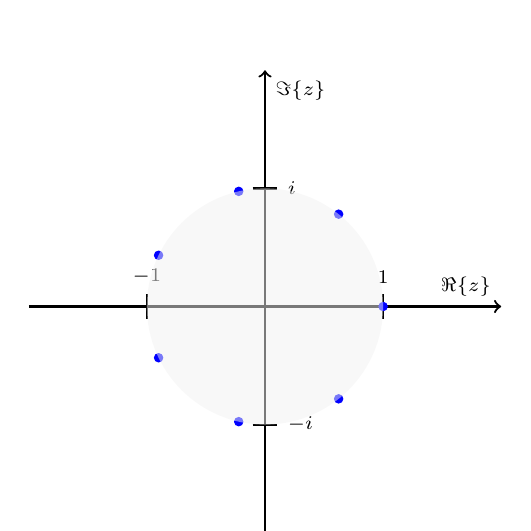
\begin{tikzpicture}[scale=1.5]
        \begin{scope}[thick,font=\scriptsize]
            % Axes:
            % Are simply drawn using line with the `->` option to make them arrows:
            % The main labels of the axes can be places using `node`s:
            \draw [->] (-2,0) -- (2,0) node [above left]  {$\Re\{z\}$};
            \draw [->] (0,-2) -- (0,2) node [below right] {$\Im\{z\}$};
        
            % Axes labels:
            % Are drawn using small lines and labeled with `node`s. The placement can be set using options
            %\iffalse% Single
            % If you only want a single label per axis side:
            \draw (1,-3pt) -- (1,3pt)   node [above] {$1$};
            \draw (-1,-3pt) -- (-1,3pt) node [above] {$-1$};
            \draw (-3pt,1) -- (3pt,1)   node [right] {$i$};
            \draw (-3pt,-1) -- (3pt,-1) node [right] {$-i$};
            %\else% Multiple
            % If you want labels at every unit step:
            %\foreach \n in {-4,...,-1,1,2,...,4}{%
                %\draw (\n,-3pt) -- (\n,3pt)   node [above] {$\n$};
                %\draw (-3pt,\n) -- (3pt,\n)   node [right] {$\n i$};
            %}
            %\fi
            \end{scope}

            \foreach \n in {0,1,2,...,6}{%
                \filldraw [blue] ({cos((360*\n)/7)}, {sin((360*\n)/7)}) circle (1pt);
                %\draw (\n,-3pt) -- (\n,3pt)   node [above] {$\n$};
                %\draw (-3pt,\n) -- (3pt,\n)   node [right] {$\n i$};
            }
            % The circle is drawn with `(x,y) circle (radius)`
            % You can draw the outer border and fill the inner area differently.
            % Here I use gray, semitransparent filling to not cover the axes below the circle
            \path [draw=none,fill=gray!10,semitransparent] (0,0) circle (1);
            % Place the equation into the circle:
            %\node [below right,gray] at (+1,-1) {$|z-1+i| \leq 3$};
    \end{tikzpicture}
    \caption{Sedmi koreni enote}
\end{figure}

To je bil le poseben primer naslednjega izreka.

\begin{izrek}[Osnovni izrek algebre]
    Obseg $\C$ je algebraično zaprt oz. vsak nekonstanten polinom $p(z)$ s kompleksnimi koeficienti ima vsaj eno ničlo v $\C$, t.j. obstaja $a \in \C$, da je $p(a) = 0$.
\end{izrek}

\begin{posledica}
    Vsak polinom $p(z)$ s kompleksnimi koeficienti in stopnje $n \in \N$ ima $n$ ničel štetih s kratnostjo. To pomeni, da lahko $p(z)$ razcepimo na produkt $n$ linearnih faktorjev
    $$p(z) = a_n(z-\alpha_1)\cdots(z-\alpha_n),$$
    kjer je $a_n \neq 0$ vodilni koeficient polinoma, $\alpha_1,\cdots,\alpha_n$ pa so njegove ničle.
\end{posledica}

\begin{opomba}
    S tem, da smo $\R$ dodali rešitev enačbe $x^2 + 1=0$, smo uspeli rešiti vse polinomske enačbe $p(z) = 0$, kjer $p(z)$ ni konstanten.
\end{opomba}

\clearpage
%\begin{center}
    \section{MNOŽICE IN PRESLIKAVE}
%\end{center}

Sistem teorije množic je ZFC (Zermelo-Fraenkel + aksiom izbire). Definirajmo nekaj osnovnih operacij med množicami $A,B \subseteq U$

\begin{definicija}
    $U$ je neka univerzalna množica objektov, o katerih govorimo: velja $A \subseteq U$ oz. $A$ je podmnožica množice $U$.
\end{definicija}

\begin{definicija}
    $A$ je podmnožica množice $B$, natanko tedaj ko so vsi elementi $A$ hkrati v $B$: $$A \subseteq B \iff \forall a: (a \in A \implies a \in B).$$
\end{definicija}

\begin{definicija}
    Množici $A$ in $B$ sta enaki, ko vsebujeta natanko enake elemente: $$A = B \iff A \subseteq B \wedge B \subseteq A.$$
\end{definicija}

\begin{definicija}
    Prazna množica je množica, ki ne vsebuje nobenega elementa. Označimo jo s simbolom $\emptyset$ in zanjo velja: $\emptyset \subseteq A,\ \forall A.$
\end{definicija}

\begin{definicija}
    Unija množic $A$ in $B$ je množica vseh elementov, ki so v $A$ ali v $B$: $$A \cup B = \{x \in U;\ x \in A \vee x \in B\}.$$
\end{definicija}

\begin{definicija}
    Presek množic $A$ in $B$ je množica vseh elementov, ki pripadajo $A$ in $B$: $$A \cap B = \{x \in U;\ x \in A \wedge x \in B\}.$$
\end{definicija}

\begin{definicija}
    Komplement množice $A$ je množica vseh elementov $U$, ki ne pripadajo $A$: $$\stcomp{A} = \{x \in U;\ x \notin A\},\ A \cup \stcomp{A} = U,\ A \cap \stcomp{A} = \emptyset.$$
\end{definicija}

\begin{definicija}
    Množici $A$ in $B$ sta disjunktni, če velja $A \cap B = \emptyset$.
\end{definicija}

\begin{definicija}
    Razlika množic $A$ in $B$ je: $$A \setminus B = \{x \in U;\ x\in A \wedge x \notin B\} = A \cap \stcomp{B}$$
\end{definicija}

\begin{izrek}[Distributivnost unije in preseka]
    Za poljubne množice $A,B,C$ veljata naslednji identiteti: 
    \begin{align*}
        (A \cup B)\cap C = (A\cap C) \cup (B\cap C)\\
        (A \cap B)\cup C = (A \cup C) \cap (C \cup C)
    \end{align*}
\end{izrek}

\begin{zgled}
    $$A \cup B = (A\cap B) \cup (A \setminus B) \cup (B \setminus A)$$
\end{zgled}
%%%%%%%%%%%%
\def\firstcircle{ (0.0, 0.0) circle (1.5)}
\def\secondcircle{(2.0, 0.0) circle (1.5)}
\def\thirdcircle{ (1.0,-1.5) circle (1.5)}
\colorlet{circle edge}{black}
\colorlet{circle area}{blue!30}

\tikzset{filled/.style={fill=circle area},
    outline/.style={draw=circle edge, thick}}

\begin{figure}
    \centering
    \begin{tikzpicture}
        \begin{scope}
            \clip \secondcircle;
            \fill[filled] \thirdcircle;
        \end{scope}

        \begin{scope}
            \clip \firstcircle;
            \fill[filled] \thirdcircle;
        \end{scope}

        \draw \firstcircle  node[left]  {$A$};
        \draw \secondcircle node[right] {$B$};
        \draw \thirdcircle  node[below] {$C$};
    \end{tikzpicture}
    \caption{Vennov diagram množice $(A\cap C) \cup (B\cap C)$}
\end{figure}
%%%%%%%%%%%%%%%
\begin{posledica}
    Posplošitev na več množic ($I$ je indeksna množica, $A_{\alpha} \subseteq U$ za $\forall \alpha \in I$).
    \begin{align*}
        \bigcup_{\alpha \in I} A_{\alpha} &= \{x \in U;\ \exists \alpha \in I,\ x \in A_{\alpha}\}\\
        \bigcap_{\alpha \in I} A_{\alpha} &= \{x \in U;\ \forall \alpha \in I,\ x \in A_{\alpha}\}
    \end{align*}
\end{posledica}
\unskip
\begin{definicija}
    Potenčna množica množice $X$ je množica, katere elementi so vse podmnožice $X$ (vključno z $\emptyset$ in $X$): 
    $$P(X) = \{A;\ A \subseteq X\}$$
\end{definicija}

\subsection{Preslikave med množicami}

\begin{definicija}
    Preslikava množice $X$ v množico $Y$ je pravilo, ki vsakemu elementu $x \in X$ priredi natanko določen element $y \in Y$. 
    Uporabimo lahko funkcijsko pisavo $f: X \rightarrow B$ oziroma $x \mapsto f(x)$ -- to pomeni, da $f$ vsakemu $x \in X$ priredi $f(x) \in Y$.
\end{definicija}

Preslikava je natanko določena s pravilom $f$ in množicama $X,Y$. Če spremenimo eno izmed teh lastnosti, dobimo drugo preslikavo. Če je $Y$ množica števil, se preslikava imenuje tudi funkcija.
$f: X \rightarrow \R$ je npr. realna funkcija na $X$, $f: X \rightarrow \C$ pa kompleksna funkcija na $X$.

Pogosto opazujemo preslikave, ki niso definirane na vsem $X$, ampak le na neki podmnožici $D \subseteq X$.

\begin{definicija}
    Domena preslikave $f: X \rightarrow Y$ je taka podmnožica $D \subseteq X$, na kateri je $f$ definirana. Običajno za domeno vzamemo največjo tako podmnožico $D$.
\end{definicija}

\begin{definicija}
    Zaloga vrednosti preslikave $f: X \rightarrow Y$ je taka podmnožica $Z_f \subseteq Y$, ki vsebuje slike vseh elementov iz domene: $Z_f = \{y \in Y; \exists x \in X: f(x) = y\} = \{f(x); x\in X\}$
\end{definicija}

\begin{definicija}
    Preslikava $f: X \rightarrow Y$ je injektivna, če za $\forall x_1,x_2 \in X$ velja $$x_1 \neq x_2 \implies f(x_1) \neq f(x_2)$$ oziroma ekvivalentno
    $$f(x_1) = f(x_2) \implies x_1 = x_2.$$ Enačba $f(x) = b$ ima največ eno rešitev za nek $b \in Y$.
\end{definicija}

\begin{definicija}
    Preslikava $f:X \rightarrow Y$ je surjektivna, če velja $Z_f = Y$ oz. za $\forall y \in Y$ obstaja $x \in X$, da velja $f(x) = y.$ Enačba $f(x) = b$ ima vsaj eno rešitev za nek $b \in Y$.
\end{definicija}

\begin{definicija}
    Preslikava $f: X \rightarrow y$ je bijektivna, če je hkrati injetivna in surjektivna. Taki funkciji rečemo tudi bijekcija iz $X$ na $Y$.
    Enačba $f(x) = b$ ima natanko eno rešitev za nek $b \in Y$.
\end{definicija}

\begin{definicija}
    Če je $f: X \rightarrow Y$ bijektivna, obstaja inverzna preslikava $f^{-1}: Y \rightarrow X$ oz. $y \mapsto f^{-1}(x) = x$, da je to natanko tisti $x \in X$, da je $f(x)=y$.
\end{definicija}

\begin{definicija}
    Kompozitum preslikav $g: Y \rightarrow Z$ in $f: X \rightarrow Y$ je funkcija $g \circ f : X \rightarrow Z$ s predpisom $(g \circ f)(x) = g(f(x))$
\end{definicija}

\begin{opomba}
    Če lahko tvorimo $g \circ f$, to še ne pomeni, da lahko tvorimo tudi $f \circ g$. Kompozitum v splošnem ni komutativna operacija. Iz množice vase $f: X \rightarrow X$ in $g: Y \rightarrow Z$ obstajata $g \circ f$ in $f \circ g$.
\end{opomba}

\begin{definicija}
    Identiteta ali identična preslikava na množici $X$ oziroma 
    $Id_x : X \rightarrow X$ je dana s predpisom $Id_X (x) = x$ za poljuben $x \in X$.
    Če je $f: X \rightarrow Y$ bijekcija in $f^{-1}: Y \rightarrow X$ njen inverz, potem velja $f^{-1} \circ f = Id_x$ in $f \circ f^{-1} = Id_y$
\end{definicija}

\subsection{Moč množic}

\begin{definicija}
    Moč množice $A$ lahko razumemo kot ">število elementov"< v $A$. 
    \begin{enumerate}
        \item Ekvipolenca množic oz. $|A| = |B|$ velja natanko tedaj, ko obstaja bijekcija $f: A \rightarrow B$. Takrat rečemo, da sta množici ekvipolentni.
        \item Neenakost $|A| \leq |B|$ velja natanko tedaj, ko obstaja injektivna preslikava $f: A \rightarrow B$, $|A| < |B|$ pa tedaj, ko med funkcijama obstaja le injektivna preslikava, ki ni bijekcija.
    \end{enumerate}
\end{definicija}

\begin{opomba}
    Lastnosti bijektivnih preslikav:
    \begin{enumerate}
        \item Za poljubno množico $A$ velja $|A| = |A|$ za $Id_A$.
        \item Če je $f: A \rightarrow B$ bijektivna, je tudi njen inverz $f^{-1}: B \rightarrow A$ bijekcija.
        \item Če je $|A| = |B|$ in $|B| = |C|$, potem je tudi $|A| = |C|$, saj je kompozitum bijekcij tudi bijekcija.
    \end{enumerate}
\end{opomba}

\begin{definicija}
    Množica $A$ je končna, če je ekvipolentna množici $\{1,2,3,\cdots,n\}$ za nek $n \in \N$. Tedaj rečemo $|A|=n$.
\end{definicija}

\begin{definicija}
    Množica $A$ je števna (tudi števno neskončna), če je ekvipolentna množici naravnih števil $\N$. Tako obstaja bijekcija $a: \N \rightarrow A$ oz. $n \mapsto a(n) = a_n$.
    Množico $A$ lahko tedaj zapišemo kot $A = \{a_1,a_2,\cdots\}$ oz njene elemente razvrstimo v zaporedje.
\end{definicija}

\begin{opomba}
    Množica $A$ je kvečjemu števna, če je ali končna ali števna.
\end{opomba}

\begin{definicija}
    Množica $A$ je kontinuum, če je ekvipolentna množici $\R$.
\end{definicija}

\begin{opomba}
    Če za množice $A,B,C$ velja $|A| \leq |B|$ in $|B| \leq |C|$, potem velja $|A| \leq |B|$, saj je kompozitum dveh injektivnih funkcij tudi injektiven.
\end{opomba}

\begin{izrek}    
    Za poljubni dve množici velja $|A| \leq |B|$ ali $|A| \geq |B|$ (posledica Zornove leme, ki je ekvivalentna aksiomu izbire.)
\end{izrek}

\begin{izrek}[Cantor-Bernstein-Schroeder]
    Če za množici $A,B$ velja $|A| \leq |B|$ in $|A| \geq |B|$, potem velja tudi $|A|=|B|$.
\end{izrek}

\begin{izrek}
    Množica racionalnih števil je števna: $|\Q| = |\N|$
\end{izrek}

    \begin{dokaz}
        Racionalna števila $$\Q = \left\{\frac{p}{q}; p \in \Z, q \in \N \right\}$$ razvrstimo v tabelo in jih nato zaobjamemo, tako da lahko tvorimo bijekcijo med $\Q$ in $\N$.
        $$a_1 = 0, a_2 = -1, a_3 = -\frac{1}{2}, a_4 = \frac{1}{2}, a_5 = 1, a_6 = -2, a_7 = -\frac{2}{3}, \cdots$$
        Podvojitve seveda izločimo, da imamo injektivnost, hkrati pa je poljubno racionalno število v sliki nekega naravnega števila in imamo surjektivnost.
    \end{dokaz}

\begin{izrek}
    Naj bo za vsak $n\in \N$ množica $A_n$ števno neskončna. Potem je unija $$A = \bigcup _{n=1} ^{\infty} A_n$$ števno neskončna (števna unija števnih množic je tudi števna).
\end{izrek}

    \begin{dokaz}
        Izrek dokažemo podobno kot prej. Ker so vse množice $A_n$ števno neskončne, lahko njihove elemente zapišemo kot injektivno zaporedje. Sedaj lahko tvorimo novo zaporedje:
        $$a_{11}, a_{21}, a_{22}, a_{12}, a_{31}, a_{32}, a_{33}, a_{23}, a_{13}, \dots,$$ ki vsebuje vse elemente unije $A = \bigcup _{n=1} ^{\infty} A_n$ (če množice $A_n$ niso paroma disjunktne ponovno izločimo podvojene elemente).
    \end{dokaz}

\begin{opomba}
    Seveda je tudi množica $\Z$ števno neskončna, saj zanjo lahko bijektivno zaporedje: 
    $$a_n = \begin{cases}
        \frac{n-1}{2};& \text{n je liho}\\
        -\frac{n}{2};& \text{n je sodo}
    \end{cases}$$
\end{opomba}

\begin{izrek}
    Kartezični produkt končno mnogo števno neskončnih množic je tudi števno neskončnen. Če so $A_1,A_2,\dots A_n,\ n \in \N$ števne množice, je števna tudi množica $$P = A_1 \times A_2 \times \dots \times A_n.$$
\end{izrek}

    \begin{dokaz}
        Dovolj je, da dokažemo za $n = 2$, saj za ostala naravna števila velja z indukcijo (med $A_1 \times A_2 \times A_3$ in $(A_1 \times A_2)\times A_3$ obstaja očitna bijekcija).
        Naj bosta A in B števni množici. Če zapišemo elemente $P = A \times B$ v tabeli, lahko po diagonalah tvorimo zaporedje: 
        \begin{equation*}
            (a_1, b_1), (a_1,b_2), (a_2, b_1), (a_3, b_1), (a_2, b_2), \dots \qedhere
        \end{equation*}
    \end{dokaz}

\begin{posledica}
    Množica algebraičnih števil je števna.

    \begin{dokaz}
        Naj bo $n \in \N$. Vseh polinomov stopnje $n$ s celoštevilskimi koeficienti je števno mnogo, saj je vsak tak polinom 
        $$p(x) = a_n x^n + a_{n-1} x^{n-1} + \dots + a_1 x + a_0,$$
        za $a_n \neq 0$ in $a_j \in \Z$ enolično določen z $(n+1)$-terico celih števil:
        $$(a_n, a_{n-1}, \dots a_1,a_0) \in \underbrace{\Z \times \Z \times \dots \times \Z}_{\text{n+1 faktorjev}}$$
        kjer $a_n \neq 0$. Vsak tak polinom definira največ $n$ algebraičnih števil, torej je množica vseh algebraičnih števil, ki so ničle kakšnega celoštevilskega koeficienta stopnje $n$, števna. Sedaj pa naredimo unijo po vseh $n \in \N$ in po prejšnjem izreku dobimo, da je množica vseh algebraičnih števil števna.
    \end{dokaz}
\end{posledica}

\begin{opomba}
    Množica transcendentnih števil je kontinuum.
\end{opomba}

\begin{izrek}
    Vsaka podmnožica $\N$ je bodisi končna bodisi števno neskončna.
\end{izrek}

    \begin{dokaz}
        Naj bo $A \subseteq \N,\ A \neq \emptyset$. Uredimo elemente $A$ po velikosti.
        $$m_1 = \inf A = \min A,\ m_2 = \min A \setminus \{m_1\},\ m_3 = \min A \setminus \{m_1, m_2\}, \dots$$
        Tako lahko $A$ zapišemo kot $A = \{m_1 < m_2 < \cdots\}.$ Če se to konča, je A končna, če pa ne, smo elemente $A$ zapisali v zaporedju: $|A| = |\N|$.
    \end{dokaz}

\begin{izrek}
    Množica $\R$ ni števna: $|\N| < |\R|$
\end{izrek}

\begin{dokaz}
        Očitno velja $|\N| \leq |\R|$, saj je $\N \subseteq \R$ in $f:n \mapsto n$ je injektivno zaporedje.

        Sedaj predpostavimo, da velja $|\R| = |\N|$. To pomeni, da lahko vse elemente $\R$ zapišemo v zaporedju, kar pa seveda pomeni, da lahko vse elemente na intervalu $X = [0,1) \in \R$ prav tako zapišemo v zaporedju.
        Vsak $x_j \in X$ zapišemo v decimalnem zapisu $$x_j = 0,n_{1j} n_{2j} n_{3j} \dots,$$
        kjer $n_{ij} \in \{0,1,2,\dots,9\}$ in decimalni zapis se ne konča z neskončno mnogo $9$.
        Sedaj definiramo $$N_j = \begin{cases}
            0; &\text{če je}\ n_{jj} \neq 0\\
            1; &\text{če je}\ n_{jj} = 0
        \end{cases}$$
        Naj bo $x = 0, N_1 N_2 N_3 \ldots$ Očitno velja $x \in [0,1) = X.$ Tedaj za vsak $j \in \N$ velja $x \neq x_j,$ kar je protislovje. Tako smo dokazali, da ne velja $|\N| = |\R|$, torej sledi $|\N|$
    \end{dokaz}

\begin{izrek}
    Za vsako množico $X$ je $|X| < |P(X)|$
\end{izrek}

    \begin{dokaz}
        Za $A \subseteq X$ definiramo karakteristično funkcijo množice $A$
        $$f_A (x) = \begin{cases}
            1;& x \in A\\
            0;& x \notin A
        \end{cases}$$
        Sedaj definiramo množico $F = \{f:X \rightarrow \{0, 1\}\},$ za katero velja $|F| = |P(X)|$, ker obstaja bijekcija $A \in P(X) \mapsto f_A \in F$.
        Vemo, da mora veljati $|X| \leq |F|$, saj
        med množicama $X$ in $F$ obstaja injektivna preslikava $x \in X \mapsto f_{\{x\}} \in F$.

        Dokažimo še $|X| \neq |F|$ s protislovjem: naj bo $|X| = |F|$. Potem obstaja bijekcija
            $\Theta(x): X \rightarrow F.$
            Za vsak $x \in X$ je $\Theta(x) \in F$ funkcija z vrednostmi $0$ ali $1$: za poljubna $x,y \in X$ je
            $(\Theta(x))(y) \in \{0,1\}.$
            Definirajmo funkcijo $\Psi(x): X \rightarrow \{0,1\}$ kot
            $$\Psi(x) = \begin{cases}
                1; &\text{če je}\ (\Theta(x))(x) = 0\\
                0; &\text{če je}\ (\Theta(x))(x) = 1
            \end{cases}$$
            Tedaj hkrati velja $\Psi \in F$ in $\Psi \neq \Theta(x)$ za $\forall x \in X$, kar je protislovje. Torej bijekcija med $X$ in $F$ ne obstaja, iz česar sledi $|X| < |F|$.
        Ker smo dokazali $|F| = |P(X)|$ in $|X| < |F|$, sledi $|X|<|P(X)|$.
    \end{dokaz}

\begin{opomba}
    Potenčna množica množice naravnih števil je kontinuum: $|\R| = |P(\N)|$.
    Pri razmisleku si lahko pomagamo z dvojiškim zapisom.
\end{opomba}

\clearpage
%\begin{center}
    \section{ŠTEVILSKA ZAPOREDJA}
%\end{center}

\begin{definicija}
    Naj bo $A \neq \emptyset$. Zaporedje v $A$ je preslikava $a: \N \rightarrow A,$ kjer $n$-ti člen zaporedja lahko zapišemo $a(n)=a_n$. Elementi oz. členi zaporedja se lahko tudi ponavljajo. Zaporedje zapišemo kot $(a_n)_{n=1} ^{\infty}$. Za nas bo $A = \R$ ali $A \subseteq \R$ (realno zaporedje).
\end{definicija}

\begin{definicija}
    Podzaporedje danega zaporedja dobimo tako, da vzamemo le nekatere člene zaporedja. Tvorimo strogo naraščajoče zaporedje naravnih števil
    $1=n_1 < n_2 < n_3 < \cdots$, kjer je $n_j \in \N.$
    Podzaporedje, ki pripada temu določenemu zaporedju, je:
    $$a_{n_1},a_{n_2},a_{n_3}, \dots = (a_{n_j})_{j=1} ^{\infty}$$
\end{definicija}

\begin{zgled}
    Zgledi nekaterih zaporedij
    \begin{enumerate}
        \item Aritmetično zaporedje: za neka $a,d \in \R$ je
        $a_n = a + (n-1)d,\ n \in \N$
        \item Geometrijsko zaporedje: za neka $a,q \in \R$ je
        $a_n = aq^{n-1},\ n \in \N$
        \item Zaporedje $a_n = \sqrt[n]n$
        \item Zaporedje $a_n = \left(1 + \frac{1}{n} \right)^n$
    \end{enumerate}
\end{zgled}

%\begin{comment}
\begin{figure}[hbt!]
    \centering
    \begin{tikzpicture}
        \begin{axis}[
            xmin=0, xmax=6,
            ymin=-1, ymax=5,
            xtick={1,2,3,4,5},
            ytick={0,1,2,3,4}
            %ymajorgrids=true,
            %grid style=dashed,
        ]
        %\addplot[domain=0.0001:5] {x^(1/x)};
        
        \addplot[dashed, color=gray, domain=0:6] {1};

        \addplot[only marks,
        color=red,
        mark=o,
        ]
        coordinates {
        (1,1)(2,{sqrt(2)})(3,{3^(1/3)})(4,{2^(1/2)})(5,{5^(1/5)})
        };

        \end{axis}
    \end{tikzpicture}
    \caption{Zaporedje $a_n = \sqrt[n]n$}
\end{figure}

\begin{figure}[hbt!]
   \centering
    \begin{tikzpicture}
        \begin{axis}[
            xmin=0, xmax=6,
            ymin=-1, ymax=5,
            xtick={1,2,3,4,5},
            ytick={0,1,2,3,4}
            %ymajorgrids=true,
            %grid style=dashed,
        ]
        %\addplot[domain=0.0001:5] {(1+1/x)^(x)};
        
        \addplot[dashed, color=gray, domain=0:6] {e};

        \addplot[only marks,
        color=red,
        mark=o,
        ]
        coordinates {
        (1,2)(2,{(3/2)^2})(3,{(4/3)^(3)})(4,{(5/4)^(4)})(5,{(6/5)^5})
        };

        \end{axis}
    \end{tikzpicture}
    \caption{Zaporedje $a_n = \left(1 + \frac{1}{n} \right)^n$}
\end{figure}
%\end{comment}
\subsection{Stekališča zaporedij}

\begin{definicija}
    Naj bo $(a_n)_{n=1} ^{\infty}$ zaporedje. Število $a\in \R$ je stekališče tega zaporedja, če za vsak $\varepsilon > 0$ in $n_0 \in \N$ obstaja tako naravno število $n \geq n_0$, da velja $|a_n - a| <\varepsilon$. Ta trditev je ekvivalentna naslednjima dvema:
    \begin{enumerate}
        \item Število $a$ je stekališče zaporedja $(a_n)_{n=1} ^{\infty}$, če za vsak $\varepsilon > 0$ v epsilonski okolici $a$ leži neskončno mnogo členov zaporedja.
        \item V vsaki okolici števila $a$ ležijo členi zaporedja s poljubno visokimi indeksi -- za noben $\varepsilon >0$ množica $\{n; |a_n -a|< \varepsilon\}$ ni navzgor omejena.
    \end{enumerate}
\end{definicija}

\begin{zgled}
    Zgledi stekališč zaporedij

    \begin{enumerate}
        \item Zaporedje $1,1,2,1,2,3,1,2,3,4,1,\dots$ ima stekališča v vseh naravnih številih.
        \item Zaporedje vseh racionalnih števil je primer zaporedja, katerega stekališča so vsa realna števila.
    \end{enumerate}
\end{zgled}

\begin{definicija}
    Naj bo $A$ množica in $f: A \rightarrow \R$ realna funkcija. Funkcija $f$ je navzgor omejena, če je $Z(f)$ navzgor omejena v $\R$ t.j. 
    obstaja $M \in \R$, da je za $\forall x \in A$ $f(x) \leq M$. Funkcija $f$ je navzdol omejena, če je $Z(f)$ navzgor omejena v $\R$ t.j.
    obstaja $m \in \R$, da je za $\forall x \in A$ $f(x) \geq m$. Funkcija $f$ je omejena, če je navzgor in navzdol omejena.
\end{definicija}

\begin{izrek}[Bolzano-Weierstrass]
    Vsako omejeno zaporedje ima vsaj eno stekališče.
    \label{izr:1}
\end{izrek}

\begin{lema}
            Če je $\zap{a}$ omejeno zaporedje, potem obstaja supremum za množico $$E = \{x \in \R;\ \text{$a_n < x$ velja za končno mnogo indeksov $n \in \N$}\}.$$
        \end{lema}
        \begin{dokaz}
        Naj bo $(a_n)_{n=1} ^{\infty}$ omejeno zaporedje. Potem obstaja tak $M \in \R,\ M \geq 0$, da za $\forall n \in \N$ velja $-M \leq a_n \leq M.$
        Naj bo $\alpha = \sup E$. Dokazati moramo, da za poljuben $\varepsilon > 0$ na intervalu $(\alpha - \varepsilon, \alpha + \varepsilon)$ leži neskončno mnogo členov zaporedja $(a_n)_{n=1} ^{\infty}$.
            Število $\alpha$ je zgornja meja za množico $E$, kar pomeni, da obstaja neskončno mnogo členov zaporedja $(a_n)_{n=1} ^{\infty}$, ki ležijo levo od $\alpha + \varepsilon$. 
            Prav tako je $\alpha$ natančna zgornja meja za $E$, torej obstaja tak $x \in E$, da velja $\alpha - \varepsilon < x \leq \alpha$. Torej levo od $x$ leži končno mnogo členov zaporedja $(a_n)_{n=1} ^{\infty}$.
            Ker levo od $\alpha + \varepsilon$ leži neskončno mnogo členov zaporedja $(a_n)_{n=1} ^{\infty}$, levo od $x$ pa leži končno mnogo členov zaporedja $(a_n)_{n=1} ^{\infty}$, sledi sklep, da na intervalu $[x, \alpha + \varepsilon)$ leži neskončno mnogo členov zaporedja $(a_n)_{n=1} ^{\infty}$.
            Zaradi relacije $[x, \alpha + \varepsilon) \subseteq (\alpha - \varepsilon, \alpha + \varepsilon)$ velja, da na intervalu $(\alpha - \varepsilon, \alpha + \varepsilon)$ leži neskončno mnogo členov zaporedja $(a_n)_{n=1} ^{\infty}$. 
    \end{dokaz}
    
\begin{dokaz}[Dokaz leme]
            Dokazati moramo, da je $E$ neprazna in navzgor omejena. Ker velja $-M \in E$, je $E$ neprazna.
            Naj bo $x>M$. Potem za $\forall n \in \N$ velja $a_n < x$, iz česar sledi $x \notin E$. Torej je $M$ zgornja meja za $E$.
            Po Dedekindovemu aksiomu ima $E$ supremum. 
        \end{dokaz}


\begin{opomba}[Limes superior in limes inferior.]
        Iz konstrukcije je razvidno, da $(a_n)_{n=1} ^{\infty}$ nima manjšega stekališča. Torej je $\alpha$ najmanjše stekališče zaporedja $(a_n)_{n=1} ^{\infty}$ oziroma \textbf{limes inferior.}
        Za vsak $\varepsilon >0$ je členov $a_n$ manjših od $\alpha - \varepsilon$ končno mnogo, členov $a_n$ manjših od $\alpha + \varepsilon$ pa neskončno mnogo. Velja torej 
        $$\liminf_{n \to \infty} a_n = \sup \{ x \in \R;\ a_n < x \text{ velja za končno mnogo indeksov}\ n \in \N\}.$$
        Podobno obstaja največje stekališče $\beta$ oziroma \textbf{limes superior.}
        Za vsak $\varepsilon >0$ je členov $a_n$ večjih od $\alpha + \varepsilon$ končno mnogo, členov $a_n$ večjih od $\alpha - \varepsilon$ pa neskončno mnogo. Velja 
        $$\limsup_{n \to \infty} a_n = \inf \{ x \in \R;\ a_n > x \text{ velja za končno mnogo indeksov}\ n \in \N\}.$$
        Od tod pa sledi, da vsako stekališče za $(a_n)_{n=1} ^{\infty}$ leži na intervalu $[\alpha, \beta] = [\liminf_{n \to \infty} a_n, \limsup_{n \to \infty} a_n].$
\end{opomba}

\subsection{Limite zaporedij}

\begin{definicija}
    Število $a \in \R$ je limita zaporedja $(a_n)_{n=1} ^{\infty}$, 
    če za $\forall \varepsilon>0$ obstaja $n_0 \in \N$, da za $\forall n \geq n_0$ velja $|a_n - a| < \varepsilon.$
\end{definicija}

\begin{opomba}
    V epsilonski okolici limite zaporedja ležijo vsi členi zaporedja razen končno mnogo, v epsilonski okolici stekališča zaporedja pa leži neskončno mnogo členov zaporedja. 
\end{opomba}

\begin{posledica}
    Če je $a$ limita zaporedja $(a_n)_{n=1} ^{\infty}$, potem je $a$ tudi stekališče zaporedja.
\end{posledica}

\begin{definicija}
    Če ima $(a_n)_{n=1} ^{\infty}$ limito, rečemo, da je konvergentno in konvergira k $a$. To zapišemo kot $\lim_{n \to \infty} a_n = a$.
\end{definicija}

\begin{izrek}
    Zaporedje $(a_n)_{n=1} ^{\infty}$ je konvergetno natanko tedaj, ko je $(a_n)_{n=1} ^{\infty}$ omejeno in ima natanko eno stekališče.
\end{izrek}

    \begin{dokaz}
        $(\Rightarrow)$ Dokažimo najprej ekvivalenco v desno.
        Naj bo $(a_n)_{n=1} ^{\infty}$ zaporedje, ki konvergira k $a$. 
        Najprej moramo dokazati omejenost. Naj bo $\varepsilon = 1$. Potem obstaja tak $n_0 \in \N$, da za $\forall n \geq n_0$ velja $a_n \in (a - 1, a+1).$ Tako lahko najdemo zgornjo in spodnjo mejo:
            $$M = \max \{a_1, a_2, \dots, a_{n_{0}-1}, a+1\},\quad m = \min \{a_1, a_2, \dots, a_{n_{0}-1}, a-1\}$$
            Vemo tudi že, da je limita zaporedja $(a_n)_{n=1} ^{\infty}$ sama po sebi stekališče. Dokazati želimo, da $(a_n)_{n=1} ^{\infty}$ nima nobenega drugega stekališča. Denimo nasprotno.
            Predpostavimo, da je $b \neq a$ stekališče zaporedja $(a_n)_{n=1} ^{\infty}$. Vzemimo poljuben $\varepsilon < \frac{1}{2} |a-b|$. Tedaj velja, da sta intervala $(a - \varepsilon, a + \varepsilon)$ in $(b-\varepsilon, b + \varepsilon)$ disjunktna.
            Potem po definiciji limite na intervalu $(a - \varepsilon, a + \varepsilon)$ ležijo vsi razen končno mnogo členov zaporedja $(a_n)_{n=1} ^{\infty}$. To pomeni, da jih na intervalu $(b - \varepsilon, b + \varepsilon)$ leži kvečjemu končno mnogo, kar pa nasprotuje predpostavki, da je $b$ stekališče. Torej je limita zaporedja $(a_n)_{n=1} ^{\infty}$ njegovo edino stekališče.

        $(\Leftarrow)$ Sedaj moramo trditev dokazati še v drugo smer.
        Naj bo $(a_n)_{n=1} ^{\infty}$ omejeno zaporedje z enim samim stekališčem v $a$. Dokazati moramo, da ima $(a_n)_{n=1} ^{\infty}$ tudi limito.
        Denimo nasprotno.
        Naj bo $\varepsilon>0$. Če $(a-\varepsilon, a+\varepsilon)$ ne vsebuje vseh členov zaporedja od nekega indeksa dalje, obstaja neskončno mnogo členov zaporedja $(a_n)_{n=1} ^{\infty}$, ki ležijo zunaj intervala $(a-\varepsilon, a + \varepsilon)$. Naj te členi tvorijo podzaporedje $(a_{n_{j}})_{j=1} ^{\infty}$. To podzaporedje je omejeno z mejami prvotnega zaporedja in ima po \ref{izr:1} stekališče, ki ga označimo z $b$. Ker po konstrukciji velja
        $|a_{n_{j}}-a| \geq \varepsilon$, sledi $|b-a| \geq \varepsilon$ in $b \neq a.$ Ker pa je $b$ stekališče podzaporedja $(a_{n_{j}})_{j=1} ^{\infty}$, je hkrati tudi stekališče zaporedja $(a_n)_{n=1} ^{\infty}$. Torej ima $(a_n)_{n=1} ^{\infty}$ dve različni stekališči $a$ in $b$, kar pa je v nasprotju z našo predpostavko. Torej je $a$ limita zaporedja $(a_n)_{n=1} ^{\infty}$.
    \end{dokaz}

\begin{posledica}
    Omejeno zaporedje $(a_n)_{n=1} ^{\infty}$ ima limito natanko tedaj, 
    ko velja $$\liminf_{n \to \infty} a_n = \limsup_{n \to \infty} a_n.$$
\end{posledica}

\begin{izrek}
    Naslednji izjavi sta ekvivalentni za zaporedje $(a_n)_{n=1} ^{\infty}$
    \begin{enumerate}
        \item Število $a \in \R$ je stekališče zaporedja $(a_n)_{n=1} ^{\infty}$.
        \item Obstaja podzaporedje $(a_{n_{j}})_{j=1} ^{\infty}$ zaporedja $(a_n)_{n=1} ^{\infty}$, ki konvergira k $a$ oziroma:
        $\lim_{j \to \infty} a_{n_j} = a$.
    \end{enumerate}
\end{izrek}

    \begin{dokaz}
        $(\Rightarrow)$ Dokažimo najprej ekvivalenco v desno.
        Naj bo $\lim_{j \to \infty} a_{n_j} = a$ za neko podzaporedje $(a_{n_j})_{j=1} ^{\infty}$. Dokazati moramo, da je $a$ stekališče zaporedja $(a_n)_{n=1} ^{\infty}$.
        Za poljuben $\varepsilon>0$ velja, da v epsilonski okolici števila $a$ ležijo vsi razen končno mnogo členov podzaporedja $(a_{n_j})_{j=1} ^{\infty}$. To pa tudi pomeni, da v epsilonski okolici števila $a$ leži neskončno mnogo členov zaporedja $(a_n)_{n=1} ^{\infty}$. Ker smo izbrali poljuben $\varepsilon$, po definiciji sledi, da je $a$ stekališče zaporedja $(a_n)_{n=1} ^{\infty}$.

        $(\Leftarrow)$ Sedaj pa še v drugo smer. Naj bo $a$ stekališče zaporedja $(a_n)_{n=1} ^{\infty}$ in naj bo $(\varepsilon_n)_{n=1} ^{\infty}$ padajoče zaporedje pozitivnih števil, za katerega velja
        $\lim_{n \to \infty} \varepsilon_n = 0$.
        Potem za epsilonske okolice $a$ za vsak $n \in \N$ velja
        $$(a- \varepsilon_{n+1}, a + \varepsilon_{n+1}) \subseteq (a - \varepsilon_n, a+ \varepsilon_n)$$
        Temu pravimo zaporedje vloženih okolic točke $a$.
        Ker je $a$ stekališče zaporedja $(a_n)_{n=1} ^{\infty}$, obstaja tako naraščajoče zaporedje naravnih števil
        $$n_1 < n_2 < n_3 < \dots,$$ da za $\forall j \in \N$ velja $|a_{n_j} - a| < \varepsilon_j$.
        Ker je $\lim_{n \to \infty} \varepsilon_n = 0$, za poljuben $\varepsilon>0$ velja, da obstaja tak $j_0 \in \N$, da za vsak $j \in \N,\ j\geq j_0$ velja
        $0 < \varepsilon_j < \varepsilon.$
        Če upoštevamo še prvo neenačbo, vidimo, da za vsak $j \geq j_0$ velja
        $|a_{n_j}-a| < \varepsilon_j < \varepsilon$ in iz tega sledi $\lim_{j \to \infty} a_{n_j} = a.$
    \end{dokaz}

\begin{posledica}
    Vsako omejeno zaporedje $(a_n)_{n=1} ^{\infty}$ ima konvergentno podzaporedje $(a_{n_j})_{j=1} ^{\infty}$.
\end{posledica}

\subsection{Monotona zaporedja}

\begin{definicija}
    Naj bo $(a_n)_{n=1} ^{\infty}$ zaporedje realnih števil. 
    \begin{enumerate}
        \item Zaporedje $\zap{a}$ je naraščajoče, če za $\forall n \in \N$ velja $a_n \leq a_{n+1}$
        \item Zaporedje $\zap{a}$ je padajoče, če za $\forall n \in \N$ velja $a_n \geq n_{n+1}$
        \item Zaporedje $\zap{a}$ je monotono, če je ali naraščajoče ali padajoče.
    \end{enumerate}
\end{definicija}

\begin{izrek}
    Če je zaporedje omejeno in monotono, ima limito.
    \begin{enumerate}
        \item Če je $(a_n)_{n=1} ^{\infty}$ naraščajoče in navzgor omejeno, je $$\lim_{n \to \infty} a_n = \sup \{a_1, a_2, a_3, \dots\}$$
        \item Če je $(a_n)_{n=1} ^{\infty}$ padajoče in navzdol omejeno, je $$\lim_{n \to \infty} a_n = \inf \{a_1, a_2, a_3, \dots\}$$
    \end{enumerate}
\end{izrek}

    \begin{dokaz}
        Dokažimo prvo točko izreka, saj je pri drugi dokaz enak. 
        Naj bo $(a_n)_{n=1} ^{\infty}$ naraščajoče in navzgor omejeno. Množica $\{a_1, a_2, \dots\}$ je očitno neprazna in omejena, zato ima supremum $a = \sup a_n$
            Naj bo $\varepsilon>0$ poljuben. Iz definicije supremuma sledi, da obstaja tak $n_0 \in \N$, da velja
            $a - \varepsilon < a_{n_0} \leq a$.
            Ker je zaporedje naraščajoče, za vsak $n \geq n_0$ velja
            $$a - \varepsilon < a_{n_0} \leq a_n \leq a.$$ Od tod sledi $a_n \in (a - \varepsilon, a + \varepsilon)$ in $\lim_{n \to \infty} a_n = a$.
    \end{dokaz}

\begin{izrek}[Primerjalni test za konvergenco]
    Naj bodo $(a_n)_{n=1} ^{\infty}$, $(b_n)_{n=1} ^{\infty}$ in $(c_n)_{n=1} ^{\infty}$ zaporedja realnih števil, za katera za $\forall n \in \N$ velja
    $a_n \leq b_n \leq c_n$ in $\lim_{n \to \infty} a_n = \lim_{n \to \infty} c_n.$
    Potem je zaporedje $(b_n)_{n=1} ^{\infty}$ konvergetno in velja
    $$\lim_{n \to \infty}a_n = \lim_{n\to \infty} b_n = \lim_{n \to \infty} c_n.$$
\end{izrek}

    \begin{dokaz}
        Naj bo $\varepsilon>0$ in
        $\lim_{n \to \infty}a_n = \lim_{n\to \infty} c_n = \alpha$.
        Potem obstaja $n_1 \in \N$, da za $\forall n \geq n_1$ velja $|a_n - \alpha| < \varepsilon$ in 
        $n_2 \in \N$, da za $\forall n \geq n_2$ velja $|c_n - \alpha| < \varepsilon$.
        Če vzamemo $n_0 = \max \{n_1, n_2\}$, potem za vsak $n \geq n_0$ velja
        $$\alpha-\varepsilon < a_n \leq b_n \leq c_n < \alpha+\varepsilon$$ in iz tega sledi $|b_n - \alpha|< \varepsilon$.
        Ker smo vzeli poljuben $\varepsilon$, je trditev dokazana.
    \end{dokaz}

\subsection{Pravila za računanje limit zaporedij}

\begin{izrek}
    Naj bosta $(a_n)_{n=1} ^{\infty}$ in $(b_n)_{n=1} ^{\infty}$ konvergentni zaporedji. Potem so konvergentna tudi
    $$(a_n + b_n)_{n = 1} ^{\infty},\ (a_n - b_n)_{n=1} ^{\infty},\ (a_n \cdot b_n)_{n=1} ^{\infty} \text{ in } \left(\frac{a_n}{b_n}\right)_{n = 1} ^{\infty}$$
    Pozor: zadnje zaporedje je konvergentno le, če je $b_n \neq 0,\ \forall n$ in $\lim_{n \to \infty} b_n \neq 0$.
\end{izrek}

\begin{posledica}
    Pravila za računanje z limitami.

    \begin{enumerate}
        \item $\limzap{a_n} + \limzap{b_n} = \limzap{(a_n + b_n)}$
        \item $\limzap{a_n} - \limzap{b_n} = \limzap{(a_n - b_n)}$
        \item $\limzap{a_n} \cdot \limzap{b_n} = \limzap{(a_n \cdot b_n)}$
        \item $\frac{\limzap{a_n}}{\limzap{b_n}} = \limzap{(\frac{a_n}{b_n})}$
    \end{enumerate}
\end{posledica}

    \begin{dokaz}[Dokaz 1. točke]
        Naj bosta $\limzap{a_n} = a,\ \limzap{b_n} = b$ in $\varepsilon>0$.
            Zaradi pogojev obstajata taka $n_1, n_2$, da za $\forall n \geq n_1$ velja $|a_n -a|< \frac{\varepsilon}{2}$ in za $\forall n \geq n_2$ velja $|b_n -b|< \frac{\varepsilon}{2}$.
            Sedaj pa vzemimo $n_0 = \max \{n_1,n_2\}$. Za $\forall n \geq n_0:$ velja:
            \begin{align*}
                |(a_n + b_n)-(a+b)| &= |(a_n-a) + (b_n-b)|\\ 
                &\leq |a_n - a| + |b_n - b|\\
                &< \frac{\varepsilon}{2} + \frac{\varepsilon}{2} = \varepsilon \qedhere
            \end{align*}
    \end{dokaz}
        
    \begin{dokaz}[Dokaz 2. točke]
        Obstajata taka $n_1, n_2$, da za $\forall n \geq n_1$ velja $|a_n -a|< \frac{\varepsilon}{2}$ in za $\forall n \geq n_2$ velja $|b_n -b|< \frac{\varepsilon}{2}.$
            Ponovno vzemimo $n_0 = \max \{n_1,n_2\}$. Za $\forall n \geq n_0$ velja:
            \begin{align*}
                |(a_n - b_n)-(a-b)| &= |(a_n-a) + (b-b_n)|\\
                &\leq |a_n - a| + |b_n - b|\\
                &< \frac{\varepsilon}{2} +\frac{\varepsilon}{2} = \varepsilon
            \end{align*}
    \end{dokaz}

    \begin{dokaz}[Dokaz 3. točke]
        Ker je $\zap{a}$ konvergentno, mora biti tudi omejeno. Zato obstaja 
            $M \geq 0$, da je $|a_n| \leq M$ za $\forall n \in \N$.
            Ponovno obstajata taka $n_1, n_2$, da za $\forall n \geq n_1$ velja $|a_n -a|< \frac{\varepsilon}{2} \frac{1}{|b|+1}$ in za $\forall n \geq n_2$ velja $|b_n -b|< \frac{\varepsilon}{2} \frac{1}{M+1}.$
            Vzemimo $n_0 = \max \{n_1,n_2\}$ in za $\forall n \geq n_0$ velja:
            \begin{align*}
                |a_n b_n-ab| &= |a_n b_n - a_n b + a_n b -ab| \\
                &\leq |b||a_n - a| + |a_n||b_n - b|\\ 
                &< \frac{\varepsilon}{2} \frac{|b|}{|b|+1} + \frac{\varepsilon}{2} \frac{M}{M+1}\\
                &< \frac{\varepsilon}{2} + \frac{\varepsilon}{2} = \varepsilon \qedhere
            \end{align*}
    \end{dokaz}

    \begin{dokaz}[Dokaz 4. točke]
        Dovolj je dokazati, da velja $\limzap{\frac{1}{b_n}} = \frac{1}{\limzap{b_n}}$. 
            Obstajata taka $n_1, n_2$, da za $\forall n \geq n_1$ velja $|b_n -b|< \frac{|b|}{2}$ in za $\forall n \geq n_2$ velja $|b_n -b|< \frac{b^2}{2} \varepsilon$.
            Zaradi trikotniške neenakosti velja $|b_n - b| \geq |b| - |b_n|$ in zato sledi, da za $\forall n \geq n_1$ velja $\frac{|b|}{2} > |b_n - b| \geq |b| - |b_n|$ in posledično $|b_n| > \frac{|b|}{2}$.
            Za $n_0 = \max \{n_1,n_2\}$ za $\forall n \geq n_0$ velja:
            \begin{align*}
                \left| \frac{1}{b} - \frac{1}{b_n} \right| = \frac{|b_n-b|}{|b||b_n|} 
                < \frac{\frac{|b|^2}{2}\varepsilon}{\frac{|b|^2}{2}} = \varepsilon \qedhere
            \end{align*} 
    \end{dokaz}


\begin{posledica}
    Naj bo $\limzap{a_n} = a$.

    \begin{enumerate}
        \item Naj bo $k \in \N$. Tedaj je $\limzap{a_n^k} = a^k$
        \item Naj bo $k \in \Z,\ a\neq 0\ \text{in}\ a_n \neq 0,\ \forall n\in \N$. Tedaj velja $\limzap{a_n^k} = a^k$
        \item Naj bo $k \in \N,\ a > 0\ \text{in}\ a_n > 0,\ \forall n\in \N$. Tedaj velja $\limzap{\sqrt[k]{a_n}} = \sqrt[k]{a}$
        \item Naj bo $r \in \Q,\ a > 0\ \text{in}\ a_n > 0,\ \forall n\in \N$. Tedaj velja $\limzap{{a_n}^r} = a^r$
        \item Naj bo $r \in \R,\ a > 0\ \text{in}\ a_n > 0,\ \forall n\in \N$. Tedaj velja $\limzap{{a_n}^r} = a^r$
    \end{enumerate}

    Trditev (1) sledi iz pravil za računanje z limitami in indukcijo, trditev (2) sledi iz trditve (1) in trditev (4) sledi iz trditev (2) in (3).
    Dokažimo (3) in (5).

    \begin{dokaz}[Dokaz 3. točke]
        Naj bo $k \geq 2$. Označimo $\sqrt[k] {a} = \alpha,\ \sqrt[k]{a_n} = \alpha_n$ Ker je $\limzap{a_n} = a$, velja, da za poljuben $\varepsilon>0$ obstaja tak $n_0 \in \N$, da za vsak $n \geq n_0,\ n \in \N$ velja 
            $|a_n - a| < \varepsilon a^{\frac{k-1}{k}}.$ Potem za vsak $n \geq n_0$ velja:
            \begin{align*}
                |\sqrt[k] {a_n} - \sqrt[k]{a}| &= |\alpha_n - \alpha|\\
                &= \frac{|\alpha_n ^k - \alpha^k|}{\alpha_n^{k-1} + \alpha \alpha_n^{k-2} + \dots + \alpha^{k-1}}\\
                &< \frac{|\alpha_n ^k - \alpha^k|}{\alpha^{k-1}}\\
                &< \frac{\varepsilon a^{\frac{k-1}{k}}}{a^{\frac{k-1}{k}}} = \varepsilon \qedhere
            \end{align*}
        \end{dokaz}

        \begin{dokaz}[Dokaz 5. točke]
            Brez škode za splošnost privzemimo, da velja $r > 0,\ a> 1\ \text{in}\ a_n >1$ za $\forall n \in \N.$
            Ker je $\limzap{a_n} = a$, je zaporedje $\zap{a}$ omejeno. in obstaja tak $M \in \R$, da je za
            $\forall n \in \N$ $1 < a_n < M$. Od tod sledi $1 < a_n^r < M^r$ za $\forall n \in \N$. 
            Naj bosta, $r^{'},r ^{''} \in \Q$, tako da velja $r^{'} < r < r^{''}$. Od tod sledi, da za $\forall n \in \N$ velja
            $a_n ^{r^{'}} < a_n^r < a_n$.
            Ker velja $\limzap{a_n^{r^{'}}} = a^{r^{'}}$ in $\limzap{a_n^{r^{''}}} = a^{r^{''}},$
            vsa stekališča zaporedja $\zap{a}$ ležijo na intervalu $[a^{r^{'}},a^{r^{''}}]$. Ker sta $r^{'}$ in $r^{''}$ poljubna in velja
            $$a^r = \sup \{a^{r^{'}}; r^{'} \in \Q; r^{'} \leq r\} = \inf \{a^{r^{''}}; r^{''} \in \Q; r^{''} \geq r\},$$
            je $a^r$ edino stekališče zaporedja $(a_n^r)_{n=1} ^{\infty}$. Torej velja $\limzap{{a_n}^r} = a^r.$
        \end{dokaz}

\end{posledica}

\subsection{Limite nekaterih posebnih zaporedij}

\begin{izrek}
    Za zaporedje $a_n = a^n$, kjer je $|a| < 1$, velja $\limzap{a^n} = 0$.
\end{izrek}

    \begin{dokaz}
        Ker velja $0 < |a^n| = |a|^n,$ je dovolj, če trditev dokažemo le za $0 \leq a < 1$, kjer je primer $a=0$ trivialen. To lahko naredimo na dva načina.
        Prvi način: Zapišemo $b = \frac{1}{a}$, kjer je $0 < a <1$. Pri dokazu obstoja logaritma smo dokazali, da množica $\{b^n; n \in \N\}$ za $b > 1$ ni navzgor omejena. To pomeni, da za vsak $\varepsilon > 0$ obstaja tak $n_0 \in \N$, da velja
            $a^{n_0} = b^{-n_0} < \varepsilon$. Sedaj pa za vsak $n \geq n_0$ velja   
            $$a^n = b^{-n} \leq b^{-n_0} < \varepsilon$$ in s tem smo dokazali 
            $\limzap{a^n} = 0.$
        
        Drugi način: Zaporedje $a_n = a^n$ za $0 <a < 1$ je očitno padajoče in navzdol omejeno z 0, torej ima limito. Naj bo $\limzap{a^n} = \alpha \geq 0$. Potem velja
            \begin{align*}
                \alpha &= \limzap{a_{n+1}}\\
                &= \limzap{a^{n+1}}\\
                &= \limzap{a \cdot a^n}\\
                &= \limzap{a} \cdot\limzap{a^n} = a \alpha
            \end{align*}
            in ker je $a \neq 1$, sledi $\alpha = 0$. 
    \end{dokaz}

\begin{izrek}
    Za zaporedje $a_n = \frac{1}{n^s}$, kjer je $s > 0$, velja $\limzap{\frac{1}{n^s}} = 0$.
\end{izrek}

    \begin{dokaz}
        Zaradi neomejenosti naravnih števil velja, da za poljubni $\varepsilon>0$ obstaja tak $n_0$, da velja $\left( \frac{1}{\varepsilon} \right) ^{\frac{1}{s}} < n_0.$ Tedaj za vsak $n\geq n_0$ velja
        \begin{align*}
            \left( \frac{1}{\varepsilon} \right) ^{\frac{1}{s}} < n \iff \left( \frac{1}{n^s} \right) < \varepsilon
        \end{align*}
        in sledi $\limzap{\frac{1}{n^s}} = 0$.
    \end{dokaz}

\begin{izrek}
    Za zaporedje $a_n = \sqrt[n]{a}$, kjer je $a>0$, velja
    $\limzap{\sqrt[n]{a}} = 1.$
\end{izrek}

    \begin{dokaz}
        Tudi to smo že dokazali pri obstoju logaritma, ampak se da tudi na drug način.
            Naj bo $0 < a < 1$. Potem je zaporedje $\zap{a}$ očitno naraščajoče in navzgor omejeno z $1$. Torej ima $\zap{a}$ limito 
            $\limzap{a_n} = \alpha \leq 1,$ za katero po izreku velja
            $\alpha = \sup\{a_n; n \in \N\}.$ To pomeni, da za vsak $n \in \N$ velja 
            \begin{align*}
                0 < a_n = \sqrt[n]{a} \leq \alpha \implies 0< a \leq \alpha^n.
            \end{align*}
            Predpostavimo, da velja $0 < \alpha < 1$. Ker je za
            $\forall n \in \N$ $0< a \leq \alpha^n$ in velja $\limzap{\alpha^n} = 0,$ je po primerjalnem testu za konvergenco tudi 
            $a = 0,$ kar pa vodi v protislovje. Torej je bila naša predpostavka napačna in velja $\alpha = 1.$
            Za $a=1$ je izrek očiten. Vzemimo še primer $a>1$. Potem za $b = \frac{1}{a} < 1$ po prvi točki velja
            $\limzap{\sqrt[n]{b}} = 1.$ Zaradi tega velja
            \begin{align*}
                \limzap{\sqrt[n]{a}} &= \limzap{\frac{1}{\sqrt[n]{b}}}\\
                &= \frac{1}{\limzap{\sqrt[n]{b}}} = 1. \qedhere
            \end{align*}
    \end{dokaz}

    \begin{figure}[hbt!]
        \centering
        \begin{tikzpicture}
            \begin{axis}[
                xmin=0, xmax=7,
                ymin=-2, ymax=7,
                xtick={1,2,3,4,5,6},
                ytick={-1,0,1,2,3,4,5,6},
                %ymajorgrids=true,
                %grid style=dashed,
            ]
            %\addplot[domain=0.0001:5] {x^(1/x)};
            
            \addplot[dashed, color=gray, domain=-1:7] {1};
    
            \addplot[only marks,
            color=red,
            mark=o,
            ]
            coordinates {
            (1,5)(2,{sqrt(5)})(3,{5^(1/3)})(4,{5^(1/4)})(5,{5^(1/5)})(6,{5^(1/6)})
            };
    
            \end{axis}
        \end{tikzpicture}
        \caption{Zaporedje $a_n = \sqrt[n]a$ za $a =5$}
    \end{figure}

\begin{izrek}
    Za zaporedje $a_n = \frac{n^s}{a^n}$, kjer je $a>1$ in $s \in \R$, velja
    $\limzap{\frac{n^s}{a^n}} = 0$
\end{izrek}

    \begin{dokaz}
        Zaporedje lahko zapišemo z rekurzivnim zapisom:
        $$a_{n+1} = \frac{1}{a} \left(1 + \frac{1}{n}\right)^s a_n.$$
        Sedaj lahko dokažemo, da je zaporedje $\zap{a}$ od nekega člena dalje padajoče. Pokazati moramo, da obstaja tako naravno število $n_0 \in \N$, da za vsak $n \geq n_0$ velja
        $\frac{1}{a} \left(1 + \frac{1}{n}\right) ^s \leq 1$. Res, če je $s > 0$, lahko izberemo $n_0 \geq \frac{1}{a^{\frac{1}{s}} -1}$ in sedaj za $\forall n \geq n_0$ velja
        \begin{gather*}
            n \geq \frac{1}{a^{\frac{1}{s}} -1} \iff \frac{1}{a} \left(1 + \frac{1}{n}\right) ^s \leq 1.
        \end{gather*}    
        Če pa je $s \leq 0$, za vse $n \in \N$ velja
        $\frac{1}{a} \left(1 + \frac{1}{n}\right) ^s \leq 1$ in smo dokazali monotonost.       
        Ker je torej $\zap{a}$ padajoče in navzdol omejeno z $0$ (vsi členi zaporedja so pozitivni), ima limito in lahko zapišemo
        $\limzap{a_n} = \alpha.$ Od tod sledi:
        \begin{align*}
            \alpha &= \limzap{a_{n+1}}\\
            &= \limzap{\left(\frac{1}{a} \left(1 + \frac{1}{n}\right)^s a_n \right)}\\
            &= \limzap{\frac{1}{a}} \cdot \limzap{\left(1 + \frac{1}{n}\right)^s} \cdot \limzap{a_n}\\ 
            &= \frac{1}{a} \cdot 1 \cdot \alpha
        \end{align*}
        in ker je $a > 1$, mora veljati $\alpha = 0$.
    \end{dokaz}

    \begin{figure}[hbt!]
        \centering
        \begin{tikzpicture}
            \begin{axis}[
                xmin=0, xmax=7,
                ymin=-2, ymax=3,
                xtick={1,2,3,4,5,6},
                ytick={-1,0,1,2},
                %ymajorgrids=true,
                %grid style=dashed,
            ]
            %\addplot[domain=0.0001:5] {x^(1/x)};
            
            \addplot[dashed, color=gray, domain=-1:7] {0};
    
            \addplot[only marks,
            color=red,
            mark=o,
            ]
            coordinates {
            (1,{(1/4)})(2,{(1/4)})(3,{(9/64)})(4,{(1/16)})(5,{(5^2/4^5)})(6,{(6^2/4^6)})
            };
    
            \end{axis}
        \end{tikzpicture}
        \caption{Zaporedje $a_n = \frac{n^s}{a^n}$ za $a =4$ in $s =2$}
    \end{figure}

\begin{izrek}
    Za zaporedje $a_n = \sqrt[n]{n}$ velja
    $\limzap{\sqrt[n]{n}} = 1$.
\end{izrek}

    \begin{dokaz}
        Za $n > 1$ je $\sqrt[n]{n} > 1$. Naj bo 
        $\sqrt[n]{n} = 1 + p_n$ za poljuben $n$, kjer je $p_n > 0.$ Tedaj velja
        \begin{align*}
            n &= (1 + p_n)^n\\
            &= 1 + \binom{n}{1} p_n + \binom{n}{2} p_n^2 + \cdots + p_n^n\\
            &< 1 + \binom{n}{2} p_n^2\\
            &= 1 + \frac{n(n-1)}{2} p_n^2
        \end{align*}
        Od tod sledi neenačba 
        $0 < p_n < \sqrt{\frac{2}{n}}$ za poljuebn $n \in \N,\ n>1$.
        Iz limite $\limzap{\sqrt{\frac{2}{n}}} = 0$ sledi
        $\limzap{p_n} = 0$ po primerjalnem testu za konvergenco. Tako imamo:
        \begin{equation*}
            \limzap{a_n} = \limzap{\sqrt[n]{n}}
            = \limzap{(1 + p_n)}
            = \limzap{1} + \limzap{p_n} = 1. \qedhere
        \end{equation*}
    \end{dokaz}

\begin{izrek}
    Zaporedje $a_n = \left(1 + \frac{1}{n} \right)^n$ je konvergentno.
\end{izrek}

    \begin{dokaz}
        Najprej dokažimo, da je $a_n = \left(1 + \frac{1}{n} \right)^n$ naraščajoče.
            \begin{equation*}
                \begin{split}
                    \left(1 + \frac{1}{n} \right)^n &= 1 + 1 + \cdots + \binom{n}{k} \left(\frac{1}{n}\right)^k + \cdots + \left(\frac{1}{n}\right)^n\\
                &= 1 + 1 + \cdots + \frac{n \cdot (n-1)\cdots (n-k+1)}{\underbrace{n \cdot n \cdots n}_{\text{k faktorjev}}} \left(\frac{1}{k!}\right) + \cdots + \left(\frac{1}{n}\right)^n\\
                &= 1 + 1 + \cdots + \left(1-\frac{1}{n}\right) \left(1-\frac{2}{n}\right) \cdot \cdots \\
                & \quad \cdot \left(1-\frac{k-1}{n}\right) \left(\frac{1}{k!}\right) + \cdots + \left(\frac{1}{n}\right)^n\\
                &< 1 + 1 + \cdots + \left(1-\frac{1}{n+1}\right) \left(1-\frac{2}{n+1}\right) \cdot \cdots \\
                & \quad \cdot \left(1-\frac{k-1}{n+1}\right) \left(\frac{1}{k!}\right) + \cdots + \left(\frac{1}{n+1}\right)^{n+1}\\
                &= \left(1 + \frac{1}{n}\right)^{n+1}
                \end{split}   
            \end{equation*}
            Vidimo, da je za $3 \leq k \leq n$ k-ti člen v razvoju $\left(1 + \frac{1}{n}\right)^n$ manjši kot kot k-ti člen v razvoju $\left(1 + \frac{1}{n+1}\right)^{n+1}$, ki pa ima še en dodaten pozitiven člen. Zato za vse $n \in \N$ velja
            $a_n < a_{n+1}.$

        Sedaj pokažimo še, da je $a_n = \left(1 + \frac{1}{n} \right)^n$ navzgor omejeno.
            Uporabimo kar razvoj iz prejšnje točke:
            \begin{align*}
                \left(1 + \frac{1}{n} \right)^n &= 1 + 1 + \cdots + \binom{n}{k} \left(\frac{1}{n}\right)^k + \cdots + \left(\frac{1}{n}\right)^n\\
                &= 1 + 1 + \cdots + \left(1-\frac{1}{n}\right) \left(1-\frac{2}{n}\right) \cdot \cdots\\
                & \quad \cdot \left(1-\frac{k-1}{n}\right) \left(\frac{1}{k!}\right) + \cdots + \left(\frac{1}{n}\right)^n\\
                &< 1 + 1 + \cdots +  \left(\frac{1}{k!}\right) + \cdots + \left(\frac{1}{n!}\right)\\
                &< 1 + 1 + \left(\frac{1}{2!}\right) + \left(\frac{1}{3!}\right) + \cdots\\
                &< 1 + 1 + \left(\frac{1}{2}\right) + \left(\frac{1}{4}\right) + \left(\frac{1}{8}\right) +\cdots = 3.
            \end{align*}
            Zaporedje $\zap{a}$ je torej navzgor omejeno s 3. \qedhere
    \end{dokaz}

\begin{opomba}
    Limita zaporedja $a_n = \left(1 + \frac{1}{n} \right)^n$ je Eulerjevo število oz. $e$. To pomeni 
    $\limzap{\left(1 + \frac{1}{n} \right)^n} = e$.
\end{opomba}

\begin{zgled}
    Izračunajmo $\limzap{\left(1-\frac{1}{n}\right)^{-n}}.$
    \begin{align*}
        \limzap{\left(1-\frac{1}{n}\right)^{-n}} &= \limzap{\left(\frac{n-1}{n}\right)^{-n}}\\
        &= \limzap{\left(\frac{n}{n-1}\right)^{n}}\\
        &= \limzap{\left(\left(1 + \frac{1}{n-1}\right)^{n-1} \left(1 + \frac{1}{n-1}\right)\right)}\\
        &= \limzap{\left(1 + \frac{1}{n-1}\right)^{n-1}} \cdot \limzap{\left(1 + \frac{1}{n-1}\right)}\\
        &= e \cdot 1 = e
    \end{align*}
    Torej velja $$\lim_{n \to -\infty} \left(1+\frac{1}{n}\right)^{n} = \limzap{\left(1-\frac{1}{n}\right)^{-n}} = e.$$
\end{zgled}

\subsection{Cauchyjevo zaporedje}

\begin{izrek}[Cauchyjev pogoj za konvergenco zaporedij]
    Naj bo $\zap{a}$ zaporedje. Naslednji trditvi sta ekvivalentni:
    \begin{enumerate}
        \item Zaporedje $\zap{a}$ je konvergentno.
        \item Za vsak $\varepsilon>0$ obstaja tak $n_0 \in \N$, da $\forall m,n \geq n_0$ velja
        $|a_m - a_n| < \varepsilon$
    \end{enumerate}
\end{izrek}

    \begin{dokaz}
        $(\Rightarrow)$ Dokažimo najprej implikacijo v desno. 
        Naj zaporedje $\zap{a}$ konvergira k $a$ oziroma $\limzap{a_n} = a.$ 
        Za poljuben $\varepsilon>0$ obstaja tak $n_0 \in \N$, da $\forall n \geq n_0$ velja 
        $|a_n - a|< \frac{\varepsilon}{2}.$ Sedaj za poljubna $m,n \geq n_0$ velja
        \begin{align*}
            |a_n - a_m| &= |a_n - a + a - a_m|\\
            &\leq |a_n - a| + |a- a_m|\\
            &= |a_n - a| + |a_m - a|\\
            &< \frac{\varepsilon}{2} + \frac{\varepsilon}{2} = \varepsilon.
        \end{align*}
        Tako velja Cauchyjev pogoj. 
        
        $(\Leftarrow)$ Sedaj pa dokažimo še v drugo smer. 
        Naj bo zaporedje $\zap{a}$ Cauchyjevo. 
        Torej za vsak $\varepsilon>0$ obstaja tak $n_0 \in \N$, da $\forall m,n \geq n_0$ velja
        $|a_m - a_n| < \varepsilon.$
            Dokazati moramo, da je zaporedje $\zap{a}$ omejeno. Naj bo $\varepsilon=1$. Ker je zaporedje Cauchyjevo, obstaja tak $n_0 \in \N$, da za $\forall n \geq n_0$ velja
            $|a_n -a_{n_0}| < 1.$ Tedaj lahko zaporedje $\zap{a}$ določimo zgornjo in spodnjo mejo:
            \begin{align*}
                M = \max \{a_1, a_2, \dots, a_{n_0-1}, a_{n_0}+1\}\\
                m = \min \{a_1, a_2, \dots, a_{n_0-1}, a_{n_0} - 1\}.
            \end{align*}
            Ker je Cauchyjevo zaporedje $\zap{a}$ omejeno, ima stekališče $a$. 
            Dokazati moramo, da je $a$ tudi limita zaporedja. Naj bo $\varepsilon>0$. Ker je zaporedje Cauchyjevo, obstaja tak $n_0 \in \N$, da za $\forall m,n \geq n_0$ velja
            $|a_n - a_m|< \frac{\varepsilon}{2}.$ 
            Ker pa je $a$ stekališče zaporedja, lahko v epsilonski okolici $a$ najdemo člene zaporedja s poljubno visokimi indeksi. Torej obstaja tak $n_1 \geq n_0$, da velja
            $|a_{n_1} - a| < \frac{\varepsilon}{2}.$ 
            Sedaj pa $\forall n \geq n_0$ velja
            \begin{align*}
                |a_n - a| &= |a_n - a_{n_1} + a_{n_1} - a|\\
                &\leq |a_n - a_ {n_1}| + |a_{n_1} - a|\\
                &< \frac{\varepsilon}{2} + \frac{\varepsilon}{2} = \varepsilon.
            \end{align*}
            Torej je res $\limzap{a_n} = a.$ \qedhere
    \end{dokaz}

\subsection{Posplošene limite}

Sedaj bomo definirali posplošeni limiti 
$\limzap{a_n}= \infty$ in $\limzap{a_n} = -\infty.$ Operirali bomo v razširjenem sistemu realnih števil:
$\overline{\R} = \R \cup \{+\infty\} \cup \{-\infty\}.$

\begin{definicija}
    Naj bo $\zap{a}$ zaporedje. 
    \begin{enumerate}
        \item Pravimo, da $\zap{a}$ konvergira k plus neskončnosti, če za $\forall M \in \R$ obstaja tak $n_0 \in \N$, da za $\forall n \geq n_0$ velja $a_n > M$. To zapišemo: $\limzap{a_n} = +\infty,$
        \item Pravimo, da $\zap{a}$ konvergira k minus neskončnosti, če za $\forall m \in \R$ obstaja tak $n_0 \in \N$, da za $\forall n \geq n_0$ velja $a_n < m$. To zapišemo: $\limzap{a_n} = -\infty,$ 
    \end{enumerate}
\end{definicija}

\begin{zgled}
    \label{zgl:1}
    Zaporedje $a_n = n^2$ konvergira k neskončnosti oz. $\limzap{n^2} = + \infty$, zaporedje $a_n = -n$ pa k minus neskončnosti oz. $\limzap{-n} = - \infty$.
\end{zgled}

\begin{figure}[hbt!]
    \centering
    \begin{tikzpicture}
        \begin{axis}[
            xmin=0, xmax=4,
            ymin=-4, ymax=10,
            xtick={1,2,3},
            ytick={-3,-2,-1,0,1,2,3,4,5,6,7,8,9},
            %ymajorgrids=true,
            %grid style=dashed,
        ]
        %\addplot[domain=0.0001:5] {x^(1/x)};

        \addplot[dashed, color=gray, domain=-1:7] {0};

        \addplot[only marks,
        color=red,
        mark=o,
        ]
        coordinates {
        (1,1)(2,4)(3,9)
        };

        \addplot[only marks,
        color=blue,
        mark=o,
        ]
        coordinates {
        (1,-1)(2,-2)(3,-3)
        };
        \end{axis}
    \end{tikzpicture}
    \caption{Zaporedji iz zgleda \ref{zgl:1}}
\end{figure}

\begin{opomba}
    Taka zaporedja smatramo za nekonvergentna. Izraz ">konvergira k neskončnosti"< razumemo kot celoto.
\end{opomba}

Sedaj si pa poglejmo še posplošeno zgornjo in spodnjo limito.

\begin{definicija}
    Naj bo $\zap{a}$ zaporedje.
    \begin{enumerate}
        \item Posplošeni limes superior gre proti plus neskončnosti natanko tedaj, ko za $\forall M \in \R$ in za vse $n_0 \in \N$ obstaja tak $n \geq n_0$, da velja $M < a_n$.
        To je ekvivalentno temu, da zaporedje ni navzgor omejeno. Zapišemo: $\limsup_{n \to \infty} a_n = +\infty.$
        \item Posplošeni limes inferior gre proti minus neskončnosti natanko tedaj, ko za $\forall m \in \R$ in za vse $n_0 \in \N$ obstaja tak $n \geq n_0$, da velja $m > a_n$. 
        To je ekvivalentno temu, da zaporedje ni navzdol omejeno. Zapišemo: $\liminf_{n \to \infty} a_n = -\infty.$
    \end{enumerate}
\end{definicija}

\begin{opomba}
    Naj bo $E$ množica stekališč zaporedja $\zap{a}.$ Veljajo naslednje trditve:
    \begin{enumerate}
        \item Če je $\zap{a}$ navzgor omejeno in $E \neq \emptyset,$ potem je
        $\limsup_{n \to \infty} a_n = \sup E.$
        \item Če je $\zap{a}$ navzgor omejeno in $E = \emptyset$, potem je $\limsup_{n \to \infty} a_n = -\infty.$
        \item Če je $\zap{a}$ navzdol omejeno in $E \neq \emptyset,$ potem je
        $\liminf_{n \to \infty} a_n = \inf E.$
        \item Če je $\zap{a}$ navzgor omejeno in $E = \emptyset$, potem je $\liminf_{n \to \infty} a_n = \infty.$
    \end{enumerate}
\end{opomba}    

\subsection{Zaporedja kompleksnih števil}

\begin{definicija}
    Kompleksno zaporedje je preslikava $z: \N \rightarrow C,$ kjer $n$-ti člen zaporedja zapišemo $z(n)=z_n$. 
\end{definicija}

\begin{definicija}
    Zaporedje $\zap{z}$ konvergira k $\alpha \in \C$, če za poljuben $\varepsilon>0$ obstaja tak $n_0 \in \N$, da za vsak $n \geq n_0$ velja
    $$d (a_n - \alpha) = |a_n - \alpha| < \varepsilon.$$
\end{definicija}

\begin{izrek}[Limita kompleksnega zaporedja]
    Naj bo $(z_n)_{n = 1} ^{\infty}$ kompleksno zaporedje, kjer je $z_n = a_n + ib_n$ in $a_n, b_n \in \R$ za $\forall n \in \N$. 
    Zaporedje $\zap{z}$ konvergira k $a + ib$, kjer sta $a,b \in \R$, natanko tedaj, ko $\zap{a}$ konvergira k $a$ in $\zap{b}$ konvergira k $b$.
    $$\limzap{(a_n + ib_n)} = a + bi \iff \limzap {a_n} = a,\ \limzap{b_n}= b$$
\end{izrek}

    \begin{dokaz}
        $(\Rightarrow)$ Dokažemo najprej implikacijo v desno. Denimo, da velja $\limzap{z_n}= \alpha = a + bi.$ Naj bo $\varepsilon>0$. Potem  obstaja $n_0 \in \N$, da za $\forall n \geq n_0$ velja
        $d(z_n, \alpha) = |z_n - \alpha| < \varepsilon.$ Tedaj za vse $n >n_0$ velja $$\sqrt{(a_n-a)^2+(b_n-b)^2} < \varepsilon$$ in končno $|a_n - a| < \varepsilon$ ter $|b_n - b| < \varepsilon$.
        Torej je $\limzap{a_n} = a$ in $\limzap{b_n}=b.$

        $(\Leftarrow)$ Dokažimo sedaj isto trditev še v nasprotno smer. Denimo, da velja
        $\limzap{a_n} = a$ in $\limzap{b_n}=b.$
        Naj bo $\varepsilon>0.$ Potem obstaja tak $n_1 \in \N$, da za $\forall n \geq n_1$ velja $|a_n - a|< \frac{\varepsilon}{\sqrt{2}}$. 
        Seveda obstaja tudi tak $n_2 \in \N$, da za $\forall n \geq n_2$ velja $|b_n - b|<\frac{\varepsilon}{\sqrt{2}}$.
        Vzemimo $n_0 = \max\{n_1,n_2\}.$ Sedaj za $\forall n \geq n_0$ velja
        \begin{align*}
            d(z_n, \alpha) &= \sqrt{(a_n - a)^2 + (b_n - b)^2}\\
            &< \sqrt{\frac{\varepsilon^2}{2} + \frac{\varepsilon^2}{2}} = \varepsilon
        \end{align*}
        Ker je bil $\varepsilon$ poljuben, smo dokazali
        $\limzap{z_n} = \alpha = a + bi$.
    \end{dokaz}

\begin{posledica}
    Naj bosta $\zap{z}$ in $\zap{w}$ kompleksni zaporedji. Tedaj:
    \begin{enumerate}
        \item $\limzap{z_n + w_n} = \limzap{z_n} + \limzap{w_n}$
        \item $\limzap{z_n - w_n} = \limzap{z_n} - \limzap{w_n}$
        \item $\limzap{z_n \cdot w_n} = \limzap{z_n} \cdot \limzap{w_n}$
        \item $\limzap{\frac{z_n}{w_n}} = \frac{\limzap{z_n}}{\limzap{w_n}}$, če je $w_n \neq 0$ za $\forall n$ in $\limzap{w_n} \neq 0$.
    \end{enumerate}
\end{posledica}

\begin{izrek}
    Kompleksno zaporedje $\zap{z}$ je konvergentno natanko tedaj, ko je Cauchyjevo -- 
    za $\forall \varepsilon > 0$ obstaja $n_0 \in \N$, da za $\forall m,n \geq n_0$ velja $$|z_n - z_m| < \varepsilon.$$
\end{izrek}

    \begin{dokaz}
        Podobno kot v prejšnjem dokazu dokažemo, da je zaporedje $\zap{z}$ Cauchyjevo natanko tedaj, ko sta zaporedji $\zap{a}$ in $\zap{b}$ Cauchyjevi. To pa velja natanko tedaj, ko sta konvergentni.
    \end{dokaz}

\begin{zgled}
    \label{zgl:2}
    Naj bo zaporedje podano s predpisom $z_n = \left(1 + \frac{1}{2n}\right)^n + i \sqrt[n]{\frac{n^2}{n+1}}$.
        Oglejmo si zaporedje $a_n = \left(1 + \frac{1}{2n}\right)^n$:
        \begin{align*}
            \limzap{\left(1 + \frac{1}{2n}\right)^n} = \limzap{\left(1 + \frac{1}{2n}\right)^{2n \cdot \frac{1}{2}}}
            = e^{\frac{1}{2}}
        \end{align*}
        Sedaj izračunajmo še limito drugega zaporedja $b_n =\sqrt[n]{\frac{n^2}{n+1}}$:
        \begin{align*}
            \limzap{\sqrt[n]{\frac{n^2}{n+1}}} &= \frac{\limzap{\sqrt[n]{n^2}}}{\limzap{\sqrt[n]{n+1}}}\\
            &= \frac{\limzap{{\sqrt[n]{n}}^2}}{\limzap{\sqrt[n]{n+1}}}\\
            &= \frac{1}{1} = 1
        \end{align*}
        Zadnji korak sledi iz tega, ker velja
        $\limzap{\sqrt[n]{n}}=1.$ Limito v imenovalcu lahko določimo z oceno in izrekom o sendviču:
        $$\sqrt[n]{n} < \sqrt[n]{n+1} \leq \sqrt[n]{2n} = \sqrt[n]{2} \cdot \sqrt[n]{n}.$$ 
    Torej velja $\limzap{z_n} = e^{\frac{1}{2}} +i.$
\end{zgled}

\begin{figure}[hbt!]
    \centering
    \begin{tikzpicture}[scale=1.5]
        \begin{scope}[thick,font=\scriptsize]
            % Axes:
            % Are simply drawn using line with the `->` option to make them arrows:
            % The main labels of the axes can be places using `node`s:
            \draw [->] (-1,0) -- (3,0) node [above left]  {$\Re\{z\}$};
            \draw [->] (0,-1) -- (0,3) node [below right] {$\Im\{z\}$};
        
            % Axes labels:
            % Are drawn using small lines and labeled with `node`s. The placement can be set using options
            %\iffalse% Single
            % If you only want a single label per axis side:
            %\draw (1,-3pt) -- (1,3pt)   node [above] {$1$};
            %\draw (-1,-3pt) -- (-1,3pt) node [above] {$-1$};
            %\draw (-3pt,1) -- (3pt,1)   node [right] {$i$};
            %\draw (-3pt,-1) -- (3pt,-1) node [right] {$-i$};
            %\else% Multiple
            % If you want labels at every unit step:
            \foreach \n in {1,2,...,2}{%
                \draw (\n,-3pt) -- (\n,3pt)   node [above] {$\n$};
                \draw (-3pt,\n) -- (3pt,\n)   node [right] {$\n i$};
            }
            %\fi
            \end{scope}

            \foreach \n in {1,2,...,20}{%
                \filldraw ({(1 + 1/(2 * \n))^(\n)}, {((\n^2)/(\n + 1))^(1 / \n)}) circle (0.5pt);
                %\draw (\n,-3pt) -- (\n,3pt)   node [above] {$\n$};
                %\draw (-3pt,\n) -- (3pt,\n)   node [right] {$\n i$};
            }

            \draw[dashed, color=gray] (-1, 1) -- (3, 1) node [above] {1};
            \draw[dashed, color=gray] ({e^(1/2)}, -1) -- ({e^(1/2)}, 3) node [right] {$e^{\frac{1}{2}}$};

            % The circle is drawn with `(x,y) circle (radius)`
            % You can draw the outer border and fill the inner area differently.
            % Here I use gray, semitransparent filling to not cover the axes below the circle
            %\path [draw=none,fill=gray!10,semitransparent] (0,0) circle (1);
            % Place the equation into the circle:
            %\node [below right,gray] at (+1,-1) {$|z-1+i| \leq 3$};
    \end{tikzpicture}
    \caption{Prvih 20 členov zaporedja iz zgleda \ref{zgl:2}}
\end{figure}

%%%%%%%%%%%%%%%%%%%%%%%%%%%%%%%%%%%%%%%%%%%%%%%%%%%%%%

\clearpage
%\begin{center}
    \section{FUNKCIJE REALNE SPREMENLJIVKE IN ZVEZNOST}
%\end{center}

\begin{definicija}
    Naj bo X množica. Funkciji $f: X \rightarrow \R$ pravimo realna funkcija,
    funkciji $f: X \rightarrow \C$ pa kompleksna funkcija.
\end{definicija}

Opazovali bomo le primere, ko velja $X = D_f \subseteq \R.$

\subsection{Graf funkcije}

\begin{definicija}
    Naj bo $f: D \subseteq \R \rightarrow \R$ funkcija.
    Graf funkcije $f$ je podmnožica $\R^2$:
    $$G(f) = \left\lbrace (x,y)\in \R^2,\ x \in D,\ y = f(x) \right\rbrace$$
\end{definicija}

Množica $\R^2 \subseteq \Gamma$ je graf funkcije 
natanko tedaj, ko vsaka navpična premica $x=a$ seka $\Gamma$ v največ eni točki. Če $\Gamma$ zadošča tej lastnosti, je graf funkcije $f$ oz. $\Gamma = G(f)$, kjer je $f$ definirana na množici $D=\Pi_x(\Gamma)$.

\begin{definicija}
    Projekcija na $x$-os je funkcija $\Pi_x : \R^2 \rightarrow \R$ s predpisom $(x,y) \mapsto x.$
\end{definicija}

\begin{definicija}
    Projekcija na $y$-os je funkcija $\Pi_y : \R^2 \rightarrow \R$ s predpisom $(x,y) \mapsto y.$
\end{definicija}

\begin{definicija}
    Naj bo $f$ funkcija in $\Gamma = G(f)$ njen graf. Definicijsko območje funkcije $f$ je $\Pi_x (\Gamma).$
\end{definicija}

Vrednost $f$ v točji $x \in D = \Pi_x(\Gamma)$ je določena s pogojem 
$(x,f(x)) \in \Gamma,$ saj je edino presečišče $\Gamma$ in navpične premice skozi $X$.

\begin{zgled}
    Krožnica $x^2 + y^2 = 1$ ni graf nobene funkcije, lahko pa jo razdelimo na dva dela:
    \begin{align*}
        \Gamma_1 &= \left\lbrace (x,y)\in \R^2; x^2 + y^2 = 1, y \geq 0 \right\rbrace\\
        \Gamma_2 &= \left\lbrace (x,y)\in \R^2; x^2 + y^2 = 1, y \leq 0 \right\rbrace
    \end{align*}
    To sta grafa funkcij $\Gamma_1 = G \left( \sqrt{1-x^2} \right)$ in $\Gamma_2 = G \left( -\sqrt{1-x^2} \right)$ na intervalu $D_{f_1} = D_{f_2} = [-1,1]$.
\end{zgled}

\begin{opomba}
    Funkcija $f$ je injektivna natanko tedaj, ko vsaka vodoravna premica $y=b$ seka graf $G(f)$ največ enkrat oz. natanko tedaj, ko je
    $\Pi_y: G(f) \rightarrow\R$ injektivna.
\end{opomba}

Denimo, da je $f:D \rightarrow \R$ injektivna. Naj bo $B = Z_f$ zaloga vrednosti funkcije $f$ oz.
$B=\{f(x); x \in D\}.$ Potem je $f: D \rightarrow B$ bijekcija in ima inverz $f^{-1} : B \rightarrow D$, tako da za $x \in D,\ y \in B$ velja
$f(x) = y$ natanko tedaj, ko je $x = f^{-1}(y).$
Torej je graf inverza:
\begin{align*}
    G(f^{-1}) = \left\lbrace (y, f^{-1}(y));\ y \in B \right\rbrace
    = \left\lbrace (f(x), x);\ x \in D \right\rbrace.
\end{align*}
Naj bo $\tau: \R^2 \rightarrow \R^2$ s predpisom $(x,y) \mapsto (y,x)$
preslikava, ki točko prezrcali preko simetrale lihih kvadrantov. Tedaj je
$\tau (G(f)) = G(f^{-1}).$

\subsection{Algebraične operacije s funkcijami}

\begin{definicija}
    Naj bosta $f,g: D \rightarrow \R$ realni funkciji.
    Definiramo naslednje operacije:
    \begin{enumerate}
        \item $(f+g)(x) = f(x) + g(x)$
        \item $(f-g)(x) = f(x) - g(x)$
        \item $(f \cdot g)(x) = f(x) \cdot g(x)$
        \item $(\frac{f}{g})(x) = \frac{f(x)}{g(x)}$, ta funkcija je definirana le na množici $D_{\frac{f}{g}} = \{x \in D;\ g(x) \neq 0\}$
    \end{enumerate}
\end{definicija}

\begin{zgled}
    Polinom je vsota funkcij $a_n x^n, a_{n-1} x^{n-1}, \dots a_1 x, a_0,$ pri čemer so te funkcije produkti kontstantne funkcije in večih funkcij $Id(x) = x.$ Zapišemo:
    $$p(x) = a_n x^n + a_{n-1} x^{n-1} + \dots + a_1 x + a_0,\quad a_0, a_1, \dots a_n \in \R.$$
\end{zgled}
\vspace{-3mm}
\begin{definicija}
    Če je funkcija $f$ navzgor omejena, je
    $$
        \underset{D}{\sup f} = \sup Z_f = \sup \{f(x);\ x \in D\}
    $$
    in če je $f$ navzdol omejena, je
    $$
        \underset{D}{\inf f} = \inf Z_f = \inf \{f(x);\ x \in D\}.
    $$
    Če obstaja $a \in D$, da je $f(a) = \underset{D}{\sup f},$ potem $f$ v točki $a$ zavzame maksimum $f(a)$ oz. $\underset{D}{\max f}$.
    Če obstaja $a \in D$, da je $f(a) = \underset{D}{\inf f},$ potem $f$ v točki $a$ zavzame minimum $f(a)$ oz. $\underset{D}{\min f}$.
\end{definicija}

\subsection{Zveznost}

\begin{definicija}
    Naj bo $D \subseteq \R$ in $f: D \rightarrow \R$ funkcija. Funkcija $f$ je zvezna v $a \in D$, če za vsak $\varepsilon>0$ obstaja tak $\delta >0$, da za vsak $x \in D$, ki zadošča
    $|x-a|< \delta,$ velja tudi $|f(x) - f(a)|<\varepsilon.$
\end{definicija}
    
Z drugimi besedami: $f$ slika $(a-\delta, a+ \delta)$ v $(f(a)-\varepsilon, f(a) + \varepsilon).$

\begin{zgled}
    Preverimo zveznost nekaterih funkcij.
    \begin{enumerate}
        \item Funkcija $f(x)=x$ je v poljubni točki $a \in \R$ zvezna,
        saj si lahko za poljubni $\varepsilon > 0$ izberemo $\delta = \varepsilon.$ Če velja $|x-a|<\delta$, potem velja tudi
        $|f(x) - f(a)| = |x-a| < \delta = \varepsilon.$
        \item Funkcija $$f(x) = \begin{cases}
            0; &\text{če je}\ x \leq 0\\
            1; &\text{če je}\ x > 0\\
        \end{cases}$$
        ni zvezna v točki $a = 0$, saj vzamemo $\varepsilon = \frac{1}{2}$ in poljuben $\delta>0$ in sedaj za katerikoli $x \in (0, \delta)$ velja 
        $|f(x) - f(0)| = 1 > \frac{1}{2} = \varepsilon.$
        \item Funkcija $f(x) = \frac{1}{x}$ je zvezna v vsaki točki $a \in \R \setminus \{0\}$. V $a = 0$ ni definirana in se torej ne moremo pogovarjati o zveznosti v tej točki. Še več, funkcije $f$ ne moremo definirati
        oz. ji predpisati neko vrednost v $0$, da bi bila tudi v tej točki zvezna.
        \item Funkcija
        $f : \R \setminus \{0\} \rightarrow \R$ s predpisom $f(x) = 1$
        je zvezna v vsaki točki $a \neq 0$. Lahko jo dodefiniramo za $x = 0$, da bo zvezna tudi v tej točki, in sicer
        $f(0) = 1.$ Potem je definirana na $\R$ in zvezna v vsaki točki $a \in \R.$
        \item Funkcija $f(x) = \sin{\frac{1}{x}}$ ni definirana v točki $a = 0.$ Nje tudi ne moremo definirati tako, da bi razširitev bila zvezna v $0$. Ničle te funkcije so 
        $x = \frac{1}{k\pi},\ k \in \Z \setminus \{0\}.$ V okolici točke $x = 0$ graf te funkcije močno oscilira. Kasneje bomo pokazali, da je ta funkcija zvezna na množici $\R \setminus \{0\}.$
        \item Funkcija $f(x) = x\sin{\frac{1}{x}}$ nihanje umiri z amplitudo $x$. Definirajmo $f(0) = 0$ in sedaj lahko pokažemo, da je $f$ zvezna v $a = 0$.
        Naj bo $\varepsilon>0$ in $\delta = \varepsilon.$ Če velja $|x| = |x-0|< \delta,$ potem je
        $$|f(x) - f(0)| = \left|x \sin{\frac{1}{x}} \right| \leq |x| < \delta = \varepsilon.$$ Funkcija $f$ je torej zvezna na vsaki točki $a \in \R$.
    \end{enumerate}
\end{zgled}

\begin{figure}[hbt!]
    \centering
    \begin{tikzpicture}
        \begin{axis}[
            xmin=-2, xmax=2,
            ymin=-2, ymax=2,
            xtick={-1,0,1},
            ytick={-1,0,1},
            %ymajorgrids=true,
            %grid style=dashed,
        ]
        %\addplot[domain=0.0001:5] {x^(1/x)};
        
            \addplot[domain=-2:-0.001] {sin((180/pi)/(x))};
            \addplot[domain=2:0.001] {sin((180/pi)/(x))};
        \end{axis}
    \end{tikzpicture}
    \caption{Funkcija $f(x) = \sin\left(\frac{1}{x}\right)$}
\end{figure}

\begin{opomba}
    Funkcija $f$ ni zvezna v $a \in D$, če obstaja tak $\varepsilon>0$, da za vsak $\delta>0$ obstaja tak $x_{\delta} \in D$, da je
    $|x_{\delta} - a|<\delta$ in $|f(x_{\delta}) - f(a)| \geq \varepsilon.$
\end{opomba}

\subsection{Karakterizacija zveznosti z zaporedji}

\begin{izrek}[Karakterizacija zveznosti z zaporedji]
    Funkcija $f: D \rightarrow\R$ je zvezna v točki $a$ natanko tedaj, ko za vsako zaporedje $\zap{x} \in D$, za katerega velja
    $\limzap{x_n} = a,$ velja tudi $\limzap{f(x_n)}=f(a).$
\end{izrek}

\begin{opomba}
    Če je $f$ zvezna v $a$, velja
    $\limzap{f(x_n)} = f(\limzap{x_n})$.
\end{opomba}

\begin{dokaz}
    $(\Rightarrow)$ Dokažimo implikacijo v desno. Naj bo $f$ zvezna v $a$ in naj bo $\zap{x}$ tako zaporedje iz $D$, da je $\limzap{x_n} = a$.
    %\begin{align}
        %\label{eq:1} \tag{$*$} \limzap{x_n} = a.
    %\end{align}
    Naj bo $\varepsilon>0$. Potem obstaja tak $\delta>0$, da za $x \in D$ velja:
    $$|x-a|<\delta \implies |f(x) - f(a)| < \varepsilon.$$
    Zaradi $\limzap{x_n} = a$ obstaja tak $n_0 \in \N$, da za $\forall n\geq n_0$ velja
    $|x_n - a| < \delta,$
    torej za $\forall n \geq n_0$ velja 
    $|f(x_n)-f(a)|<\varepsilon$
    in zato sledi
    $\limzap{f(x_n)} = f(a).$

    $(\Leftarrow)$ Sedaj pa še v drugo smer. Denimo, da $f$ ni zvezna v $a$. Naj bo $\varepsilon>0$ kot v zgornji opombi. Naj bo $\delta = \frac{1}{n}$, $n \in \N$.
    Potem po zgornji opombi za $\forall n \in \N$ obstaja tak $x_n \in D$, da velja
    $$|x_n -a| < \delta = \frac{1}{n} \quad \text{in} \quad |f(x_n) -f(a)| \geq \varepsilon.$$ Tako smo našli zaporedje $\zap{x}$ iz $D$, da je 
    $\limzap{x_n} = a,$ $(f(x_n))_{n = 1} ^{\infty}$ pa ne konvergira k $f(a)$, kar pa je v nasprotju z našo predpostavko.
\end{dokaz}

\begin{definicija}
    Funkcija $f: D \rightarrow \R$ je zvezna (na $D$), če je zvezna v vsaki točki $a \in D$.
\end{definicija}

\begin{izrek}
    Naj bosta $f,g:D \rightarrow \R$ funkciji, ki sta zvezni v točki $a \in D.$ Potem so v $a$ zvezne tudi funkcije:
    $$f+g,\ f-g,\ f \cdot g,\ \frac{f}{g}.$$
    Pozor: funkcija $\frac{f}{g}$ je zvezna v $a$ le, če je tam tudi definirana oz. velja $g(a) \neq 0$.
\end{izrek}

\begin{opomba}
    Iz zgornjega izreka sledi, da je v $a$ zvezna tudi funkcija $c\cdot f,$ kjer je $c \in \R$, saj za $g$ vzamemo konstantno funkcijo $g(x) = c,$ ki je zvezna v vsaki točki.
\end{opomba}

\begin{dokaz}
    Dokažimo to trditev le za prvo in tretjo funkcijo, saj sta preostala dokaza podobna.
    Najprej dokažimo zveznost funkcije $(f+g)$ v $a$.
    Naj bo $\varepsilon>0$. Ker je $f$ zvezna v $a$, obstaja $\delta_f >0$, da za $x \in D$ velja
        $|x-a|<\delta_f \implies |f(x) - f(a)|<\frac{\varepsilon}{2}.$
        Ker je $g$ zvezna v $a$, obstaja $\delta_g >0$, da za $x \in D$ velja
        $|x-a|<\delta_g \implies |g(x) - g(a)|<\frac{\varepsilon}{2}.$ 
        Naj bo $\delta = \min \{\delta_f, \delta_g\}.$ Potem za $x \in D,\ |x-a|<\delta$ velja
        \begin{align*}
            |(f+g)(x) - (f+g)(x)| &= |(f(x) - f(a)) + (g(x)-g(a))|\\
            &\leq |f(x) - f(a)| + |g(x) - g(a)|\\
            &\leq \frac{\varepsilon}{2} + \frac{\varepsilon}{2} = \varepsilon
        \end{align*}
        Dokažimo še zveznost funkcije $(f \cdot g)$.
        Naj bo $\zap{x}$ zaporedje iz $D$, da je $\limzap{x_n} = a.$ Ker sta $f$ in $g$ zvezni funkciji, po karakterizaciji zveznosti z zaporedji velja:
        $\limzap{f(x_n)} = f(a)$ in $\limzap{g(x_n)} = g(a).$
        %\begin{align*}
         %   \limzap{f(x_n)} &= f(a)\\
          %  \limzap{g(x_n)} &= g(a)
        %\end{align*}
        Iz tega sledi:
        \begin{align*}
            \limzap{(f \cdot g)(x_n)} &= \limzap{f(x_n) g(x_n)}\\
            &= \limzap{f(x_n)} \cdot \limzap{g(x_n)}\\
            &= f(a) \cdot g(a) = (f \cdot g)(a)
        \end{align*}
        Torej je $(f \cdot g)$ zvezna v $a$.
\end{dokaz}

\begin{posledica}
    Naj bodo funkcije $f_1,\dots,f_n$ zvezne na $D$. Tedaj sta tudi funkciji $f_1 + \dots + f_n$ in $f_1 \cdot \ldots \cdot f_n$ zvezni na $D$.
    Dokaz sledi z indukcijo.
\end{posledica}

\begin{izrek}
    Kompozitum zveznih funkcij je zvezna funkcija. Naj bo $f:D \rightarrow G$ zvezna v $a$ in $g:G \rightarrow \R$ zvezna v $b = f(a) \in G$. Tedaj je
    $g \circ f: D \rightarrow \R$ zvezna v $a \in D$.
\end{izrek}

    \begin{dokaz}
        Izrek bomo dokazali z zaporedji.
        Naj bo $\zap{x}$ zaporedje v $D$, da je 
        $\limzap{x_n} = a.$ Potem mora veljati
        $\limzap{f(x_n)} = f(a),$ saj je $f$ zvezna v $a$. Torej je
        $\limzap{g(f(x_n))} = g(f(a)),$ saj je $g$ zvezna v $f(a) = b.$ Od tod pa sledi:
        $$\limzap{(g \circ f)(x_n)} = (g \circ f)(a)$$ in $g \circ f$ je zvezna v $a$.
    \end{dokaz}

\begin{zgled}
    Podajmo nekaj zgledov zveznih funkcij.

    \begin{enumerate}
        \item Konstantne funkcije so zvezne povsod na $\R$.
        \item Funkcija $f(x) = x$ je zvezna povsod na $\R$.
        \item Polinomi $$p(x) = a_n x^n + a_{n-1} x^{n-1} + \dots + a_1 x + a_0,$$ kjer je $n \in \N$ in $a_n,\dots,a_0 \in \R$, so zvezni na $\R$.
        \item Racionalne funkcije $\frac{p(x)}{q(x)}$, kjer sta $p,q$ polinoma, so zvezne na celotnem definicijskem območju $\R \setminus\{x; q(x) =0\}$.
        \item Eksponentna funkcija $f(x) = b^x$, $b >0$, je zvezna na $\R.$
        \item Sinusna funkcija je zvezna na $\R$.
        Posledično je $\cos x = \sin{\left( \frac{\pi}{2}-x \right)}$ zvezna na $\R$ (po pravilu zveznosti kompozituma dveh zveznih funkcij),
        $\tan x = \frac{\sin x}{\cos x}$ je zvezna na $\R \setminus \left\lbrace \frac{\pi}{2} + k\pi; k \in \Z \right\rbrace$ in $\cot x = \frac{\cos x}{\sin x}$ je zvezna na $\R \setminus \left\lbrace k\pi; k \in \Z \right\rbrace$.
    \end{enumerate}
\end{zgled}

\begin{dokaz}[Dokaz 5. točke]
            To smo že dokazali pri obstoju logaritma. Naj bo 
            $f(x) = b^x$ za nek $b >1$.
            Sedaj velja $|f(x) - f(a)| = |b^a||b^{x-a}-1|$.
            Naj bo $\varepsilon>0$. Iščemo $\delta>0$, da velja
            $$|x-a|<\delta \implies |b^{x-a}-1|<\frac{\varepsilon}{b^a}.$$ 
            Vemo že, da velja
                $\limzap{b^{\frac{1}{n}}} = 1.$
                Torej obstaja tak $n_0 \in \N$, da za $\forall n \geq n_0$ velja
                $|b^{\frac{1}{n}} - 1| < \frac{\varepsilon}{b^a}.$
                Od tod velja, da iz $0 \leq x-a < \frac{1}{n_0}$ sledi $$0 \leq b^{x-a} - 1 < b^{\frac{1}{n_0}} -1 < \frac{\varepsilon}{b^a}.$$
            Sedaj se približajmo limiti še iz druge strani. Tokrat uporabimo limito $\limzap{b^{-\frac{1}{n}}} = 1.$
                Torej obstaja tak $n_1 \in \N$, da za $\forall n \geq n_1$ velja
                $|b^{-\frac{1}{n}} - 1| < \frac{\varepsilon}{b^a}.$
                Od tod velja, da iz $0 \geq x-a > -\frac{1}{n_1}$ sledi $$0 \leq |b^{x-a} - 1| < 1 - b^{-\frac{1}{n_1}}  < \frac{\varepsilon}{b^a}$$
            Naj bo $\delta = \frac{1}{\max\{n_0, n_1\}}.$ Sedaj za $x$, za katerega velja
            $|x-a|<\delta,$ velja tudi
            $|b^{x-a} - 1|<\varepsilon b^{-a}$ oz. $|b^x - b^a| < \varepsilon$.
            Če je $0 < b < 1$, potem lahko zlahka prevedemo na prejšnji primer s pomočjo kompozituma.
        \end{dokaz}

            \begin{lema} 
                \label{lem:4}
                Za vsak $x \in \R$ velja
                $|\sin x| \leq x$. Trditev ima geometrijski dokaz, ki smo ga že srečali v gimnaziji.
            \end{lema}

        \begin{dokaz}[Dokaz 6. točke]
            Za dokaz bomo uporabili lemo \ref{lem:4}.
            Naj bo $a \in \R$. Potem velja
            \begin{align*}
                |\sin x - \sin a| &= 2|\sin {\frac{x-a}{2}}||\cos {\frac{x+a}{2}}|\\
                &\leq 2 \cdot \frac{|x-a|}{2} \cdot 1\\
                &= |x-a|
            \end{align*}
            Naj bo $\varepsilon>0.$ Izberimo $\delta = \varepsilon$ in dobimo:
            \begin{equation*}
                |x-a| < \delta \implies |\sin x - \sin a| < \delta = \varepsilon \qedhere
            \end{equation*}
        \end{dokaz}

\begin{opomba}
    Manjka še zveznost korenov, logaritmov in ciklometričnih funkcij. Ta bo sledila iz že dokazanih zveznosti, ker so te funkcije inverzne funkcije prejšnjim.
\end{opomba}

\subsection{Monotone funkcije}

\begin{definicija}
    Naj bo $f: D \rightarrow \R$ funkcija. Funkcija $f$ je monotona, če zanjo velja vsaj ena izmed naslednjih točk:
    \begin{enumerate}
        \item $f$ je naraščajoča, če velja $$x_1 , x_2 \in D;\ x_1 \leq x_2 \implies f(x_1) \leq f(x_2)$$
        \item $f$ je padajoča, če velja $$x_1 , x_2 \in D;\ x_1 \leq x_2 \implies f(x_1) \geq f(x_2)$$
        \item $f$ je strogo naraščajoča, če velja $$x_1 , x_2 \in D;\ x_1 < x_2 \implies f(x_1) < f(x_2)$$
        \item $f$ je strogo padajoča, če velja $$x_1 , x_2 \in D;\ x_1 < x_2 \implies f(x_1) > f(x_2)$$
    \end{enumerate}
\end{definicija}

\begin{opomba}
    Povezava z injektivnostjo.
    \begin{itemize}
        \item Če je $f$ strogo monotona funkcija, je tudi injektivna.
        \item Če je $f$ zvezna injektivna funkcija na intervalu/poltraku/celi realni osi, potem je strogo monotona.
    \end{itemize}
\end{opomba}

\begin{izrek}
    Naj bo $f: I \rightarrow \R$ zvezna strogo monotona funkcija na intervalu $I$ (interval ali poltrak ali $\R$). Tedaj je njena inverzna funkcija
    $f^{-1}: J = Z_f \rightarrow I$ zvezna.
\end{izrek}

\begin{posledica} Navedimo nekaj posledic tega izreka.
    \begin{enumerate}
        \item Za vsak $n \in \N$ je funkcija $f(x) = \sqrt[n]{x}$ zvezna na $[0, \infty)$.
        To smo že dokazali pri zaporedjih, saj velja 
        $\limzap{\sqrt[k]{a_n}} = \sqrt[k]{\limzap{a_n}}$.
        Sledi pa tudi iz tega, da je to inverzna funkcija funkcije $f: I = [0, \infty) \rightarrow J = [0,\infty)$ s predpisom $f(x) = x^n$.
        
        \item Naj bo $r \in \Q.$ Funkcija $f(x) = x^r$ je zvezna na $(0,\infty).$
        Tudi to smo že dokazali pri zaporedjih. Sicer pa naj bo $r = \frac{m}{n}$, za  $m \in \Z,\ n \in \N$ in 
        $f(x)= x^r.$ To pa je kompozitum funkcij $x \mapsto x^{\frac{1}{n}}$ in $y \mapsto y^m$ in potemtakem mora biti zvezen.
        
        \item Naj bo $r \in \R.$ Funkcija $f(x) = x^r$ je zvezna na $(0,\infty).$
        Tudi to smo že dokazali pri zaporedjih. Če je
        $\limzap{a_n} = a$ za $a_n >0,\ a>0,$ potem velja
        $\limzap{a_n^r} = a^r.$ To pa je natanko pogoj za zveznost v $a$.
    \end{enumerate}
\end{posledica}        

\begin{posledica}
    Naj bo $b > 0,\ b \neq 1.$ Funkcija
        $f(x) = b^x$ je strogo monotona preslikava iz
        $\R \rightarrow (0,\infty).$ Inverzna preslikava je $\log_b : (0,\infty) \rightarrow \R$ in je po izreku zvezna funkcija.
\end{posledica}
        
\begin{posledica}
    Ciklometrične funkcije so zvezne tam, kjer so definirane.
        \begin{enumerate}
            \item Funkciji $\sin : [-\frac{\pi}{2}, \frac{\pi}{2}] \rightarrow [-1,1]$ in 
                $\arcsin : [-1,1] \rightarrow [-\frac{\pi}{2},\frac{\pi}{2}]$
            sta druga drugi inverzni. Vse rešitve enačbe $\sin x = a$, $a \in [-1,1]$ so oblike $\arcsin(a) + 2k\pi$ ali $\pi - \arcsin(a) + 2k\pi$ za poljuben $k \in \Z$.
            
            \item Funkciji
                $\cos : [0, \pi] \rightarrow [-1,1]$ in
                $\arccos : [-1,1] \rightarrow [0, \pi]$
            sta druga drugi inverzni. Vse rešitve enačbe $\cos x = a$, $a \in [-1,1]$ so oblike $\arccos(a) + 2k\pi$ ali $-\arccos(a) + 2k\pi$ za poljuben $k \in \Z$.
            
            \item Funkciji
                $\tan : (-\frac{\pi}{2}, \frac{\pi}{2}) \rightarrow \R$ in
                $\arctan : \R \rightarrow (-\frac{\pi}{2}, \frac{\pi}{2})$
            sta druga drugi inverzni. Vse rešitve enačbe $\tan x = a$, $a \in \R$ so oblike $\arctan(a) + k\pi$ za $k \in \Z$.
        \end{enumerate}
\end{posledica}

\begin{posledica}
    Funkcije, ki jih prav tako pogosto srečamo, so hiperbolične funkcije. Hiperbolični sinus in kosinus sta:
            $\sinh x = \frac{e^x-e^{-x}}{2}$ in $\cosh x = \frac{e^x + e^{-x}}{2}$.
        Ti funkciji sta obe zvezni, vendar pa je $\sinh$ liha, $\cosh$ pa soda. Za hiperbolične funkcije veljajo nekatere formule, ki veljajo že za trigonometrične formule, na primer
        $\cosh^2 - \sinh^2 = 1$.
        Posledica tega je, da je tudi funkcija
        $\tanh(x) = \frac{\sinh(x)}{\cosh(x)}$ zvezna na $\R$ (opomba: $\tanh(x)$ je definirana na celotnem $\R$, saj velja $\cosh(x) \geq 0$).
        \begin{enumerate}
            \item Funkcija $\sinh : \R \rightarrow \R$ je bijektivna. Njen inverz je funkcija area hiperbolični sinus oziroma $\textup{\text{arsinh}} : \R \rightarrow \R$ s predpisom
            $x \mapsto \ln{(x + \sqrt{x^2 + 1})}$.

            \item Funkcija $\cosh : [0, \infty) \rightarrow [1, \infty)$ je bijektivna. Njen inverz je funkcija area hiperbolični kosinus oziroma $\textup{\text{arcosh}} : [1, \infty) \rightarrow [0, \infty)$ s predpisom
            $x \mapsto \ln{(x + \sqrt{x^2 - 1})}$.

            \item Funkcija $\tanh : \R \rightarrow (-1, 1)$ je bijektivna. Njen inverz je funkcija area hiperbolični tangens oziroma $\textup{\text{artanh}} : (-1, 1) \rightarrow \R$ s predpisom
            $x \mapsto \frac{1}{2} \ln{\frac{1+x}{1-x}}$.
        \end{enumerate}
\end{posledica}

\begin{dokaz}[Dokaz izreka o zveznosti inverzne funkcije.]
    Naj bo $f: I \rightarrow J = Z_f$ zvezna, strogo monotona bijekcija na intervalu $I$ in 
    $f^{-1} : J \rightarrow I$ njen inverz. Naj bo $a \in I$ in $b = f(a) \in J$. Dokazujemo zveznost $f^{-1}$ v $b$.
    Naj bo $\varepsilon>0$. Brez škode za splošnost naj bo $f$ strogo naraščajoča in naj bo $a$ notranja točka $I$. Če je potrebno, $\varepsilon$
    zmanjšamo, da je $[a - \varepsilon, a+ \varepsilon] \subseteq I.$ Potem velja:
    $$f(a-\varepsilon) = b_{-\varepsilon} < b = f(a) < b(a+\varepsilon) = b_{+\varepsilon}$$
    Naj bo $\delta = \min\{b-b_{-\varepsilon}, b_{+\varepsilon}-b\}$. Vzemimo tak $y \in J$ tak, da je $|y-b| < \delta.$ Torej velja:
    \begin{equation}
        \label{eq:2} \tag{$*$} f(a-\varepsilon) = b_{-\varepsilon} \leq b-\delta < y < b + \delta \leq b_{+\varepsilon} = f(a+\varepsilon)
    \end{equation}
    Ker je $y \in J = Z_f$, obstaja natanko določen $x \in I$, da je $f(x) = y$ oz. $f^{-1} (y) = x.$ 
    Sedaj zaradi \eqref{eq:2} in stroge monotonosti $f$ velja:
    \begin{itemize}
        \item $x< a+\varepsilon$, saj bi v nasprotnem primeru ($x \geq a + \varepsilon$) veljalo $f(a+\varepsilon) = b_{+\varepsilon} \leq f(x),$ kar pa vodi v protislovje zaradi $|y-b|<\delta.$
        \item $x > a-\varepsilon$, saj bi v nasprotnem primeru ($x \leq a - \varepsilon$) veljalo $f(a-\varepsilon) = b_{-\varepsilon} \geq f(x),$ kar pa ponovno vodi v protislovje zaradi $|y-b|<\delta.$
    \end{itemize}
    Torej velja $a-\varepsilon < x < a+\varepsilon$.
    Da ponovimo: Za vsak $y \in J$, za katerega velja $|y-b| < \delta$, obstaja točno določen $x \in I$, da velja
    $f(x) = y$ in $|x-a| < \varepsilon.$ Torej za $\forall y \in J$ obstaja $\delta>0$, da velja
    $$|y-b| < \delta \implies |f^{-1} (y) - f^{-1} (b)| < \varepsilon$$ in funkcija $f^{-1}$ je zvezna v točki $b$.
\end{dokaz}

\subsection{Enakomerna zveznost}

Naj bo funkcija $f$ zvezna na $D$. 
Potem za vsak $\varepsilon > 0$ obstaja takšen $\delta>0$, da iz $|x-a| < \delta$ sledi $|f(x)-f(a)| < \varepsilon$, kjer je $a \in D$. 
V definiciji zveznosti je pri danem $\varepsilon>0$ izbor $\delta$ torej odvisen od $a \in D$. 
Zanima nas, če lahko najdemo podoben $\delta$, ki ne bi bil odvisen od $a$, t.j. ali bi za izbrani $\delta$ veljal pogoj zveznosti za katerikoli $a \in D$.
V splošnem to ne velja, zaradi česar uvedemo pojem enakomerne zveznosti funkcije.

\begin{zgled}
    Naredimo nekaj zgledov enakomerne zveznosti:
    \begin{enumerate}
        \item Oglejmo si funkcijo $f(x) = x^2$. Naj bo $\varepsilon>0$ in $a\in \R$ poljubna točka. 
        Zanima nas, če obstaja univerzalen $\delta>0$, da velja $|f(x)-f(a)|<\varepsilon$ za vsak $x \in D$, ki zadošča $|x-a|<\delta$.
        Vzemimo poljuben $\delta > 0$ in $x = a + \frac{\delta}{2}$. Sedaj velja $|x - a| < \delta$ in $|f(x) - f(a)| = |a \delta + \frac{\delta^2}{4}|$
        in ta izraz gre proti neskončnosti, ko gre $a$ preko vsake meje. Torej takšen $\delta$ ne obstaja.
        \item Oglejmo si $f(x) = \frac{1}{x}$ na intervalu $(0,1]$. Naj bo $\varepsilon>0.$ 
        Zanima nas, če obstaja $\delta>0$, neodvisen od $a \in (0,1]$, da velja
        $\left| \frac{1}{x} - \frac{1}{a}\right| < \varepsilon$ za $x \in (0,1]$, ki zadošča $|x-a|< \delta$? Če je $a < \delta$, potem to mora veljati za $x = \frac{a}{2}$. Sledi
        $\left|\frac{2}{a} -\frac{1}{a}\right| = \frac{1}{a} < \varepsilon,$ kar pa seveda ne velja za vse $a \in (0,1]$. Ponovno želeni $\delta$ ne obstaja.
    \end{enumerate}
\end{zgled}

\begin{definicija}
    Funkcija $f:D \rightarrow \R$ je enakomerno zvezna na $D$, če za vsak $\varepsilon>0$ obstaja $\delta>0$, da za vsak par $x,x' \in D$ velja
    $$|x-x'|< \delta \implies |f(x) - f(x')| < \varepsilon.$$
\end{definicija}

\begin{zgled}
    Za $f(x) = x$ na $\R$ vzamemo $\delta = \varepsilon$ in smo dokazali enakomerno zveznost.
\end{zgled}

\begin{izrek}
    Naj bo $D$ omejen interval in $f:D \rightarrow\R$ enakomerno zvezna. Potem je $f$ omejena na $D$.
\end{izrek}

    \begin{dokaz}
        $D$ je lahko zaprt, odprt ali polodprt interval. Naj bo $a \in D$ in $\varepsilon = 1$. Potem obstaja tak $\delta>0$, da za $x, x' \in D$ velja:
        $$|x-x'|< 2\delta \implies |f(x) - f(x')| < 1.$$ Oglejmo si točke
        $a_k = a + k \delta$ za $k \in \Z.$ Ker je $D$ omejen interval, leži na intervalu $D$ največ
        $\frac{l(D)}{\delta} + 1 = N$ takih točk. Za poljubno točko $x \in D$ obstaja $k \in \Z$, da velja 
        $a_{k-1} \leq x < a_k.$ Denimo, da je $k \geq 1.$ Potem velja:
        \begin{align*}
            |f(x) - f(a)| &\leq |f(x) -f(a_{k-1})| + \dots + |f(a_1) - f(a_0)|\\
            &< k \cdot 1 \leq N
        \end{align*}
        Tako za vsak $x \in D$ velja $$f(a) - N < f(x) < f(a) + N.$$ S tem smo pokazali, da je $f$ omejena na $D$.
    \end{dokaz}

\begin{opomba}
    Zgornji izrek ne velja nujno za poltrake ali pa $\R$. Primer: $f(x) =x$.
\end{opomba}

\begin{izrek}
    Kompozitum dveh enakomerno zveznih funkcij je enakomerno zvezna funkcija.
\end{izrek}

\subsection{Osnovne lastnosti zveznih funkcij na zaprtih omejenih intervalih.}

\begin{izrek}
    Naj bo zaprt omejen interval $D = [a,b]$, $a,b \in \R$. Če je $f:D \rightarrow \R$ zvezna na $D$, potem je tudi enakomerno zvezna na $D$.
\end{izrek}

    \begin{dokaz}
        Denimo, da $f$ ni enakomerno zvezna na $D$. Obstaja $\varepsilon>0$, da za $\forall n \in \N$ obstajata $x_n, x_n' \in D$, da velja 
        $|x_n -x_n'| < \frac{1}{n}$ in $|f(x_n) - f(x_n')| \geq \varepsilon.$

        Zaporedji $\zap{x}$ in $\zap{x'}$ sta zaporedji na zaprtem intervalu $[a,b]$ in zato imata stekališči.
        Torej obstaja podzaporedje $(x_{n_j})_{j=1} ^{\infty},$ ki konvergira k $\alpha \in [a,b]$ oziroma
            $\lim_{j \to \infty} {x_{n_j}} = \alpha.$
            Prav tako obstaja podzaporedje 
            $(x'_{n_{j_k}})_{k=1} ^{\infty},$ ki konvergira k $\beta \in [a,b]$ oziroma
            $\lim_{k \to \infty} {x'_{n_{j_k}}} = \beta.$
            Od tod sledi
            \begin{gather*}
                \lim_{k \to \infty} {x_{n_{j_k}}} = \alpha \quad \text{in} \quad 
                \lim_{k \to \infty} {x'_{n_{j_k}}} = \beta.
            \end{gather*}
        V nadaljne bomo ta sklep preskočili in zgolj brez škode za splošnost predpostavili, da obe originalni zaporedji konvergirata.
        Sedaj zaradi predpostavke
        $|x_n -x'_n| < \frac{1}{n}$ velja
        $\limzap{(x_n -x'_n)} = 0.$ Iz tega sledi
        \begin{gather*}
            \lim_{k \to \infty} {(x_{n_{j_k}} -x'_{n_{j_k}})} = 0 \quad \text{in} \quad \lim_{k \to \infty} {x_{n_{j_k}}} = \lim_{k \to \infty} {x'_{n_{j_k}}} = \alpha
        \end{gather*}
        Po drugi strani pa velja
        $|f(x_{n_{j_k}}) - f(x'_{n_{j_k}})| \geq \varepsilon$ in zato $f$ ni zvezna v točki $\alpha$ (sicer bi oba člena konvergirala proti $f(\alpha)$ -- karakterizacija zveznosti z zaporedji).
    \end{dokaz}

\begin{izrek}
    \label{izr:2}
    Naj bo $f$ zvezna na zaprtem omejenem intervalu $D = [a,b]$, $a <b$. Potem je $f$ na $D$ omejena in obstajata točki $x_m, x_M \in D$, da je
    \begin{align*}
        f(x_m) = \inf_{D} f = \min_{D} f\\
        f(x_M) = \sup_D f = \max_D f
    \end{align*}
    oz. $f$ zavzame minimum in maksimum.
\end{izrek}

\begin{zgled}
    To seveda ne velja za odprte intervale: naj bo $D = (0,1)$ in $f(x) = x$. Očitno $f$ na $D$ ne zavzame maksimuma oziroma minimuma.
\end{zgled}

\begin{dokaz}
    Zgornji izrek lahko dokažemo s kombinacijo prejšnjih dveh: $f$ je na zaprtem intervalu zvezna, zato je na zaprtem intervalu tudi enakomerno zvezna, iz enakomerne zveznosti pa sledi omejenost.

    Lahko pa trditev dokažemo tudi neposredno: naj bo $f$ navzgor neomejena. Potem za vsak $n \in \N$ obstaja $x_n \in [a,b]$, da velja: $f(x_n) > n.$
    Zaporedje $\zap{x}$ je omejeno, zato ima stekališče. Tako obstaja neko podzaporedje $(x_{n_j})_{j=1} ^{\infty}$, da velja
    $$\lim_{j \to \infty} {x_{n_j}}= \alpha \in [a,b],$$ vendar pa zaradi $f(x_{n_j}) > n_j$ zaporedje $(f(x_{n_j}))_{j = 1} ^{\infty}$ ne konvergira k $f(\alpha)$. Torej $f$ ni zvezna v točki $\alpha \in [a,b]$, kar vodi v protislovje. Identičen dokaz je za navzdol omejenost.

    Dokažimo še, da $f$ na $D$ zavzame maksimum: naj bo $M = \sup_D f.$ Če $f$ ne zavzame vrednosti $M$ na $D$, potem je funkcija $g = \frac{1}{M - f}$ zvezna na $D$. Ker pa iz definicije supremuma velja, da za vsak $\varepsilon > 0$ obstaja $x_\varepsilon \in D$, da je $M - \varepsilon < f(x_\varepsilon) < M$ in iz tega sledi $g(x_\varepsilon) > \frac{1}{\varepsilon},$ torej $g$ ni navzgor omejena na $D$. Ker pa 
    je $g$ zvezna, to privede v protislovje. Zato $f$ zavzame maksimum na $D$ in podobno sledi, da na $D$ zavzame tudi minimum.
\end{dokaz}

\begin{izrek}
    Naj bo $f: [a,b] \rightarrow \R$ zvezna. Če je $f$ v krajiščih nasprotno predznačena oz. velja
    $f(a) f(b) < 0,$ potem obstaja tak $c \in (a,b)$, da je $f(c) = 0$, tj. $f$ ima ničlo na intervalu $(a,b)$.
\end{izrek}
    
\begin{dokaz}
    Metoda bisekcije: Denimo, da je $f(a) < 0$ in $f(b) > 0$. Naj bo $a_1 = a$, $b_1 = b$ in $c = \frac{a_1 + b_1}{2}$. 
    Če je $f(c_1) = 0$, smo ničlo našli, sicer pa velja bodisi $f(c_1) < 0$ bodisi $f(c_1) > 0$.
    V prvem primeru definiramo $a_2 = c_1$, $b_2 = b_1$, v drugem pa $a_2 = a_1$, $b_2 = c_1$.
    Postopek ponovimo na intervalu $[a_2, b_2]$, kjer ponovno velja $f(a_2) f(b_2) < 0.$ Če na katerem koli koraku dobimo ničlo, postopek zaključimo. 
    Sicer dobimo dve zaporedji $\zap{a}$ in $\zap{b}$.
    Zaporedje $\zap{a}$ je naraščajoče, $\zap{b}$ pa padajoče. Za vsak $j \in \N$ velja
    \begin{equation}
        \label{eq:3}
        b_j - a_j = \frac{b-a}{2^{j-1}} \quad \text{in} \quad f(a_j) f(b_j) < 0.
    \end{equation}
    Očitno je, da iz zaporedij $\zap{a}$ in $\zap{b}$ dobimo zaporedje vloženih intervalov
    $$[a_1, b_1] \mathrel{{\reflectbox{$\subseteq$}}} [a_2, b_2] \mathrel{{\reflectbox{$\subseteq$}}} [a_3 , b_3] \dots$$
    Ker sta $\zap{a}$ in $\zap{b}$ monotoni in omejeni, obstajata limiti $\limzap{a_n} = \alpha$ in $\limzap{b_n} = \beta$.
    Iz \eqref{eq:3} sledi, da velja $\alpha = \beta = c$, torej je presek vloženih intervalov enak $$\bigcap_{n = 1} ^{\infty} [a_n, b_n] = \{c\}.$$
    Zaradi $f(a_j) f(b_j) < 0$ velja $$\limzap{f(a_n) f(b_n)} = f(c)^2 \leq 0,$$ kar pa je možno le za $f(c) = 0$. Torej smo izrek dokazali.
\end{dokaz}

\begin{posledica}
    Naj bo $f$ zvezna na omejenem zaprtem intervalu $D = [a,b]$. Potem $f$ zavzame vse vrednosti med $m = \min_D f$ in $M = \max_D f.$ 
    To pomeni, da za $\forall y \in [m, M]$ obstaja $\exists x_0 \in [a,b]$, da je $f(x_0) = y$ oziroma 
    $Z_f = f(D) = [m, M].$
\end{posledica}

\begin{dokaz}
    Naj bo $y \in [m, M]$. Za $y = M$ ali $y = m$ je trditev že dokazana z izrekom \ref{izr:2}, 
    saj obstajata $x_m, x_M \in D$, da je $f(x_M) = M$ in $f(x_m) = m$.
    Vzemimo torej $y_0 \in (m,M)$ in poglejmo funkcijo $g(x) = f(x) - y_0$ na intervalu od $x_m$ do $x_M$. 
    Potem je $$g(x_m) = m - y_0 < 0 \quad \text{in} \quad g(x_M) = M - y_0 > 0$$ ter iz izreka o bisekciji sledi, da ima funkcija $g$ na intervalu od $x_m$ do $x_M$ ničlo $x_0$.
    Ker je $$g(x_0) = f(x_0) - y_0 = 0,$$ funkcija $f$ v točki $x_0 \in D$ zavzame vrednost $y_0$.
\end{dokaz}

\begin{posledica}
    Naj bo $I$ interval ali poltrak ali $\R$ in funkcija $f: I \rightarrow \R$ zvezna in injektivna. Tedaj je $f$ strogo monotona na $I$.
\end{posledica}

\begin{dokaz}
    Naj bosta $a,b \in I,\ a<b$. Brez škode za splošnost predpostavimo, da je $f(a) < f(b)$ (enakost ne more veljati zaradi injektivnosti). 

        Naj bo $c \in I$, da velja $a < c < b$. Potem mora veljati $f(a) < f(c) < f(b)$, saj bi sicer prišli v protislovje z injektivnostjo. 
        Res, $f$ na intervalu $[c,b]$ zavzame vse vrednosti od $f(c)$ do $f(b)$. Če bi veljalo $f(c) \leq f(a)$, potem bi za nek $x_0 \in [c,b]$ bilo $f(x_0) = f(a)$. 
        Ker pa je $x_0 > a$, je to v protislovju z injektivnostjo, torej velja $f(c) > f(a)$.
        Na enak način pokažemo tudi $f(c) < f(b)$.
        
        S podobnim argumentom pokažemo tudi, da iz $b < d$ sledi $f(d) > f(b)$ in iz $e < a$ sledi $f(a) > f(e)$ za poljubna $d,e \in I$.
        Vse ostale primere lahko privedemo do zgornjih, torej smo dokazali.
\end{dokaz}

\subsection{Limite funkcij}

\begin{zgled}
    Naj bo $f(x) = \frac{\sin x}{x}$ za $x \neq 0$ in $f$ je zvezna na $\R \setminus \{0\}$. Ali bi jo lahko primerno dodefinirali v točki $x = 0$, da je zvezna na $\R$?
    Vemo že, da za $\forall x \in \left(-\frac{\pi}{2} \right) \cup \left(0, \frac{\pi}{2} \right)$ velja $\cos x \leq \frac{\sin x}{x} \leq 1.$ Ko je $x$ blizu $0$, je zaradi zveznosti $\cos x$ blizu 1. Torej je za $x \approx 0,\ x \neq 0$ vrednost izraza $\frac{\sin x}{x} \approx 1$.
    Zdi se, da bi bilo naravno definirati $f(0) = 1$.
\end{zgled}

\begin{figure}[hbt!]
    \centering
    \begin{tikzpicture}[scale=0.9]
        \begin{axis}[
            xmin=-2, xmax=2,
            ymin=-2, ymax=2,
            xtick={-1,0,1},
            ytick={-1,0,1},
            %ymajorgrids=true,
            %grid style=dashed,
        ]
        %\addplot[domain=0.0001:5] {x^(1/x)};
        
            \addplot[domain=-2:-0.001] {(sin(x*180/pi))/x};
            \addplot[domain=2:0.001] {(sin(x*180/pi))/x};
            \addplot[domain=-2:2, color=gray, dashed] {1};
            \addplot[domain=-2:2, color=gray, dashed] {0};
            \addplot[dashed, color=gray] coordinates {(0,-2)(0,2)};
            \addplot[only marks, color=red] coordinates {(0,1)};
        \end{axis}
    \end{tikzpicture}
    \caption{Funkcija $f(x) = \frac{\sin{x}}{x}$}
\end{figure}

\begin{definicija}
    Naj bo $a \in \R$ in $r > 0$. Definiramo funkcijo $f : (a-r, a+r) \setminus \{a\} \rightarrow \R$ na punktirani oz. prebodeni okolici $a$. Število $A \in \R$ je limita funkcije $f$ v točki $a$, če za $\forall \varepsilon > 0$ obstaja $\delta > 0$\footnote{Veljati mora $0 < \delta \leq r$}, da velja
    $|f(x) - A| < \varepsilon$ za vse $x$, ki zadoščajo $0 < |x-a| < \delta$. To označimo kot $A = \limf{x}{a}{f(x)}$.
\end{definicija}

\begin{trditev}
    Definicija močno spominja na definicijo zveznosti, le da $f$ v $a$ ni definirana.
    \begin{enumerate}
        \item Če je $f$ definirana na $(a-r, a+r)$ in zvezna v $a$, potem velja $\limf{x}{a}{f(x)} = f(a).$
        \item Če je $\limf{x}{a}{f(x)} = A$ in definiramo 
        $$\tilde{f}(x) = \begin{cases}
            f(x); & x \neq a\\
            A; & x = a
        \end{cases}$$ 
        je $\tilde{f}(x)$ zvezna v $a$.
    \end{enumerate}
\end{trditev}

\begin{zgled}
    Iz zgornje neenakosti $\cos x \leq \frac{\sin x}{x} \leq 1$ za $x \in \left(-\frac{\pi}{2}, \frac{\pi}{2}\right) \setminus \{0\}$ sledi:
    $\limf{x}{0}{\frac{\sin x}{x}} =1$.
\end{zgled}

\begin{opomba}
    Od tod sledi običajna aproksimacija v fiziki. Če so koti (v radianih) majhni, je $\sin x \approx x.$
\end{opomba}

\begin{zgled}
    Funkcija $f(x) = \frac{1}{x}$ je definirana na $\R \setminus \{0\}$, a nima limite v točki $0$, ker ni omejena v nobeni prebodeni okolici točke $0$.
\end{zgled}

\begin{izrek}
    Karakterizacija limite funkcije z zaporedji: za funkcijo $f: (a-r, a+r) \setminus \{a\} \rightarrow \R$ sta naslednji trditvi ekvivalentni:
    \begin{enumerate}
        \item Limita funkcije v točki $a$ je $\limf{x}{a}{f(x)} = A \in\R$.
        \item Za vsako zaporedje $\zap{x}$ iz množice $(a-r,a+r) \setminus \{a\}$, za katerega velja $\limzap{x_n} = a$, velja tudi $\limzap{f(x_n)} = A$.
    \end{enumerate}
\end{izrek}

\begin{dokaz}
    Dokaz sledi neposredno iz karakterizacije zveznosti z limitami zaporedij.
\end{dokaz}

\begin{zgled}
    Funkcija $f(x) = \sin \left( \frac{1}{x} \right),\ x \neq 0$ je zvezna na $\R \setminus \{0\}$.
    A ker za $x_n = \frac{1}{n \pi}$ velja $\limzap{f(x_n)} = 0$ ter za $x_n' = \frac{1}{\frac{\pi}{2} + 2n \pi}$ velja $\limzap{f(x_n')} = 1,$
    ne moremo dodefinirati $f$ v točki $0$ z neko vrednostjo, da bi razširjena funkcija bila zvezna.
    Torej $\limf{x}{0}{f(x)}$ ne obstaja.
\end{zgled}

Za limite funkcij v točki veljajo običajne algebraične lastnosti.

\begin{trditev}
    Naj bosta $f,g$ definirani na $(a-r, a+r) \setminus \{r\}$. Če obstajata $\limf{x}{a}{f(x)}$ in $\limf{x}{a}{f(x)},$ potem obstajajo limite:
    $\limf{x}{a}{(f+g)(x)}$, $\limf{x}{a}{(f-g)(x)}$, $\limf{x}{a}{(f \cdot g)(x)}$, $\limf{x}{a}{(\frac{f}{g})(x)}$.
    Te limite so enake:
    \begin{enumerate}
        \item $\limf{x}{a}{(f+g)(x)} = \limf{x}{a}{f(x)} + \limf{x}{a}{g(x)}$
        \item $\limf{x}{a}{(f-g)(x)} = \limf{x}{a}{f(x)} - \limf{x}{a}{g(x)}$
        \item $\limf{x}{a}{(f\cdot g)(x)} = \limf{x}{a}{f(x)} \cdot \limf{x}{a}{g(x)}$
        \item $\limf{x}{a}{(\frac{f}{g})(x)} = \frac{\limf{x}{a}{f(x)}}{\limf{x}{a}{g(x)}}$
    \end{enumerate}
    
    Pozor: limita $\limf{x}{a}{(\frac{f}{g})(x)}$ obstaja le, če je $g(a) \neq 0$.
\end{trditev}

Trditev sledi iz podobnega izreka z zveznimi funkcijami ali iz karakterizacije z limitami zaporedij.

\begin{zgled}
    Oglejmo si funkcijo $sgn (x)$:
    $$f(x) = \begin{cases}
        1;\ &x>0\\
        0;\ &x = 0\\
        -1;\ &x<0
    \end{cases}$$
    Limita $\limf{x}{0}{f(x)}$ ne obstaja, saj hkrati veljata limiti $\limzap{f(\frac{1}{n})} = 1$ in $\limzap{f(-\frac{1}{n})} = -1.$
    Zdi pa se, da če se točki $x=0$ približujemo le z ene strani, npr. z desne, se vrednost funkcije približuje vrednosti $1$.
\end{zgled}

\begin{definicija}
    Naj bo $f: (a-r, a) \rightarrow \R$ funkcija. Funkcija $f$ ima levo limito v točki $a$, če za $\forall \varepsilon>0$ obstaja $\delta >0$, da za vsak $x \in (a - \delta, a)$ velja
    $|f(x) - A| < \varepsilon.$ To označimo kot $\lim_{x \uparrow a} f(x) = A$.
\end{definicija}

\begin{definicija}
    Naj bo $f: (a, a+r) \rightarrow \R$ funkcija. Funkcija $f$ ima desno desno v točki $a$, če za $\forall \varepsilon>0$ obstaja $\delta >0$, da za vsak $x \in (a, a + \delta)$ velja
    $|f(x) - A| < \varepsilon.$ To označimo kot $\lim_{x \downarrow a} f(x) = B$.
\end{definicija}

    
\begin{zgled}
    Ponovno si oglejmo funkcijo $$f(x)= \begin{cases}
        1; &x>0\\
        0; &x = 0\\
        -1; &x<0
    \end{cases}.$$ Sedaj velja $\lim_{x \uparrow a} f(x) = -1$ in $\lim_{x \downarrow a} f(x) = 1$ in nobena od teh vrednosti ni enaka $f(0) = 0$.
\end{zgled}

\begin{opomba}
    Če je $f$ definirana na $(a-r, a+r) \setminus \{a\}$ in leva ter desna limita obstajata ter nista enaki, pravimo, da ima $f$ v $a$ skok.
\end{opomba}

\begin{trditev}
    Funkcija $f$ ima v $a$ limito natanko tedaj, ko ima v $a$ levo in desno limito in sta enaki. Tedaj velja $\limf{x}{a}{f(x)} = \llimf{x}{a}{f(x)} = \rlimf{x}{a}{f(x)}$.
\end{trditev}

Levo limito pogosto označimo z $f(a-0)$ oz. $f(a-)$, desno pa z $f(a+0)$ oz. $f(a+)$.

\begin{izrek}
    \label{thm:2}
    Naj bo $f: I \rightarrow \R$ monotona funkcija na intervalu $I$. 
    Potem ima $f$ levo in desno limito v vsaki notranji točki intervala $I$.
\end{izrek}

\begin{dokaz}
    Naj bo $f: I \rightarrow \R$ naraščajoča in naj bo $a \in I$ notranja točka. Naj bo $x < a,\ x \in I$. Potem je $f(x) \leq f(a).$ Množica $E = \{f(x); x<a, x \in I\}$ je neprazna in navzgor omejena, zato ima supremum. 
    Trdimo, da je $\llimf{x}{a}{f(x)} = \sup E.$ Naj bo $A = \sup E$ in poljuben $\varepsilon >0$. Potem obstaja tak $x_0 \in I,\ x_0 < a$, da je $$A - \varepsilon < f(x_0) \leq A.$$ Naj bo $\delta = a - x_0 > 0$.
    Če je $x \in (a - \delta, a) = (x_0, a),$ sledi $$A - \varepsilon < f(x_0) \leq f(x) \leq A$$ zaradi monotonosti. Torej za vsak $x \in (a - \delta, a)$ velja $|f(x) - A| < \varepsilon$ in
    zato je $A = \llimf{x}{a}{f(x)}.$ Podobno dokažemo 
    \begin{equation*}
        \rlimf{x}{a}{f(x)} = \inf \{f(x); x>a, x \in I\}. \qedhere
    \end{equation*}
\end{dokaz}

\begin{posledica}
    Monotona funkcija ima največ števno mnogo skokov, t.j. točk nezveznosti.
\end{posledica}

\begin{dokaz}
    Če ima $f$ v $a$ skok, izberemo neko racionalno število ne intervalu med $f(a-)$ in $f(a+)$. Denimo, da je $f$ naraščajoča. Potem je $$r_a \in (f(a-), f(a+)).$$ Naj bosta $a<b$ števili iz intervala $I$, v katerih ima $f$ skok. 
    Potem je $$f(a+) = \rlimf{x}{a}{f(x)} \leq f(b-) = \llimf{x}{b}{f(x)},$$ saj zaradi monotonosti velja $f(a+) \leq f\left(\frac{a+b}{2}\right) \leq f(b-).$ 
    Torej sta intervala $(f(a-),f(a+))$ in $(f(b-), f(b+))$ disjunktna in zato je $r_a \neq r_b.$
    Tako je preslikava iz množice skokov za $f$ v množico racionalnih števil $a \mapsto r_a$ injektivna. Torej je množica skokov za $f$ kvečjemu števna (ali števna ali končna).
\end{dokaz}

\begin{zgled}
    Izračunajmo naslednje limite:
    $$\limf{x}{0}{\frac{\tan x}{x}}, \quad \limf{x}{0}{\frac{\sin (\alpha x)}{x}}, \quad \limf{x}{0}{\frac{1 - \cos x}{x}}, \quad \limf{x}{0}{\frac{1 - \cos x}{x^2}}$$

    \begin{enumerate}
        \item $\displaystyle \limf{x}{0}{\frac{\tan x}{x}}  = \limf{x}{0}{\frac{\sin x}{x}} \cdot \limf{x}{0}{\frac{1}{\cos x}} = 1 \cdot 1 = 1$
        \item $\displaystyle \limf{x}{0}{\frac{\sin (\alpha x)}{x}} = \limf{x}{0}{\frac{\sin (\alpha x)}{\alpha x} \cdot \alpha} 
        \stackrel{\alpha x = t}{=} \limf{t}{0}{\frac{\sin t}{t} \alpha}
        = \alpha$
        \item $\displaystyle \limf{x}{0}{\frac{1 - \cos x}{x}} = \limf{x}{0}{\frac{2 \sin^2 \left( \frac{x}{2} \right)}{x}}
        = \limf{x}{0}{2 \cdot \frac{\sin \frac{x}{2}}{x} \cdot \sin \left(\frac{x}{2}\right)}
        = 0$
        \item $\displaystyle \limf{x}{0}{\frac{1 - \cos x}{x^2}} = \limf{x}{0}{\frac{2 \sin^2 \frac{x}{2}}{x^2}}
        = \limf{x}{0}{2\left( \frac{\sin \frac{x}{2}}{x} \right)^2}
        = 2 \cdot \left(\frac{1}{2}\right)^2 = \frac{1}{2}$
    \end{enumerate}
\end{zgled}
%%%%%%%%%%%%%%%%%%%%%%%%%%%%%

%%%%%%%%%%%%%%%%%%%%%%%%%%%%%

\begin{figure}
    \centering
    \begin{minipage}[b][7cm][s]{.45\textwidth}
    \centering
    \vfill
    \begin{tikzpicture}[scale=0.85]
        \begin{axis}[
            xmin=-2, xmax=2,
            ymin=-1, ymax=4,
            xtick={-1,0,1},
            ytick={0,1,2,3},
            %ymajorgrids=true,
            %grid style=dashed,
        ]
        %\addplot[domain=0.0001:5] {x^(1/x)};
        
            \addplot[domain=-1.5:-0.001] {(tan(180*x/pi))/x};
            \addplot[domain=1.5:0.001] {(tan(180*x/pi))/x};

            \addplot[domain=-2:2, color=gray, dashed] {1};
            \addplot[dashed, color=gray] coordinates {(0,-1)(0,4)};
            \addplot[only marks, color=red] coordinates {(0,1)};
        \end{axis}
    \end{tikzpicture}
    \caption{Funkcija $f(x) = \frac{\tan\left(x\right)}{x}$.}
    \end{minipage}\qquad
    \begin{minipage}[b][7cm][s]{.45\textwidth}
    \centering
    \vfill
    \begin{tikzpicture}[scale=0.85]
        \begin{axis}[
            xmin=-3, xmax=3,
            ymin=-2, ymax=3,
            xtick={-2,-1,0,1,2},
            ytick={-1,0,1,2},
            %ymajorgrids=true,
            %grid style=dashed,
        ]
        %\addplot[domain=0.0001:5] {x^(1/x)};
        
            \addplot[domain=-3:-0.001] {sin(deg(3 * x/4)))/x};
            \addplot[domain=0.001:3] {sin(deg(3 * x/4)))/x};

            \addplot[domain=-3:3, color=gray, dashed] {3/4};
            \addplot[dashed, color=gray] coordinates {(0,-2)(0,3)};
            \addplot[only marks, color=red] coordinates {(0,3/4)};
        \end{axis}
    \end{tikzpicture}
    \caption{Funkcija $\frac{\sin \left(\frac{3}{4} x \right)}{x}$.}
    \end{minipage}
    
    \begin{minipage}[b][7cm][s]{.45\textwidth}
    \centering
    \vfill
    \begin{tikzpicture}[scale=0.85]
        \begin{axis}[
            xmin=-2, xmax=2,
            ymin=-2, ymax=2,
            xtick={-1,0,1},
            ytick={-1,0,1},
            %ymajorgrids=true,
            %grid style=dashed,
        ]
        %\addplot[domain=0.0001:5] {x^(1/x)};
        
            \addplot[domain=-2:-0.05] {(1 - cos(deg(x)))/x};
            \addplot[domain=2:0.05] {(1 - cos(deg(x)))/x};

            \addplot[domain=-2:2, color=gray, dashed] {0};
            \addplot[dashed, color=gray] coordinates {(0,-2)(0,2)};
            \addplot[only marks, color=red] coordinates {(0,0)};
        \end{axis}
    \end{tikzpicture}
    \caption{Funkcija $f(x) = \frac{1 - \cos\left(x\right)}{x}$.}
    \end{minipage}\qquad
    \begin{minipage}[b][7cm][s]{.45\textwidth}
    \centering
    \vfill
    \begin{tikzpicture}[scale= 0.85]
        \begin{axis}[
            xmin=-2, xmax=2,
            ymin=-2, ymax=2,
            xtick={-1,0,1},
            ytick={-1,0,1},
            %ymajorgrids=true,
            %grid style=dashed,
        ]
        %\addplot[domain=0.0001:5] {x^(1/x)};
        
            \addplot[domain=-2:-0.05] {(1 - cos(deg(x)))/x^2};
            \addplot[domain=2:0.05] {(1 - cos(deg(x)))/x^2};

            \addplot[domain=-2:2, color=gray, dashed] {1/2};
            \addplot[dashed, color=gray] coordinates {(0,-2)(0,2)};
            \addplot[only marks, color=red] coordinates {(0,1/2)};
        \end{axis}
    \end{tikzpicture}
    {\caption{Funkcija $f(x) = \frac{1 - \cos\left(x\right)}{x^2}$.}}
    \end{minipage}
    \end{figure}
    

%%%%%%%%%%%%%%%%%%%%%%%%%%%%%

\begin{opomba}
    Iz zadnjega primera sledi, da za $x \approx 0$ velja $\cos x \approx 1 - \frac{1}{2}x^2.$
\end{opomba}

\subsection{Posplošene limite}

\begin{definicija}
    Naj bo $f$ definirana na $(a-r, a+r) \setminus \{a\}$ za $a \in \R$ in $r > 0$. 
    \begin{enumerate}
        \item Pravimo, da $f$ konvergira k $+ \infty$, ko gre $x$ proti $a$, če za $\forall M \in \R$ (še tako velik) obstaja tak $\delta > 0$\footnote{Ponovno mora veljati mora $0 < \delta \leq r$}, da velja
        $f(x) > M$ za vse $x$, ki zadoščajo $0 < |x-a| < \delta$.
        \item Pravimo, da $f$ konvergira k $- \infty$, ko gre $x$ proti $a$, če za $\forall m \in \R$ (še tako majhen) obstaja tak $\delta > 0$, da velja
        $f(x) < m$ za vse $x$, ki zadoščajo $0 < |x-a| < \delta$.
    \end{enumerate}
\end{definicija}

To zapišemo kot $\limf{x}{a}{f(x)} = + \infty$ in $\limf{x}{a}{f(x)} = - \infty.$

\begin{zgled}
    Limita funkcije $f(x) = \frac{1}{x^2}$, ko se $x$ približuje $0$, je $\limf{x}{0}{\frac{1}{x^2}} = + \infty$
\end{zgled}

Podobno definiramo posplošene enostranske limite: to so $\llimf{x}{a}{f(x)} = + \infty$, $\llimf{x}{a}{f(x)} = - \infty$, $\rlimf{x}{a}{f(x)} = + \infty$ in $\rlimf{x}{a}{f(x)} = - \infty$.

\begin{zgled}
    Oglejmo si primer posplošenih levih in desnih limit funkcij:
    \begin{enumerate}
        \item Enostranski limiti funkcije $f(x) = \frac{1}{x}$, ko se približujemo $x=0$: desna limita je
        $\rlimf{x}{0}{\frac{1}{x}} = + \infty$, leva pa $\llimf{x}{0}{\frac{1}{x}} = - \infty$
        \item Enostranski limiti funkcije $f(x) = \tan x$, ko se približujemo $x=0$: desna limita je tokrat
        $\rlimf{x}{\frac{\pi}{2}}{\tan{x}} = - \infty$, leva pa $\llimf{x}{\frac{\pi}{2}}{\tan{x}} = + \infty$
    \end{enumerate} 
\end{zgled}

\begin{definicija}
    Naj bo $f$ definirana na $(a, \infty)$; $a \in \R$. 
    Število $A \in \R$ je limita funkcije $f(x)$, ko gre $x$ proti $ + \infty$, če za $\forall \varepsilon > 0$ obstaja $M > a$, da za $\forall x > M$ velja $|f(x) - A| < \varepsilon.$
\end{definicija}

To označimo kot $\limf{x}{\infty}{f(x)} = A.$ 
Podobno definiramo tudi limito od $f$, ko gre $x$ proti minus neskončnosti: $\limf{x}{-\infty}{f(x)}.$

\begin{zgled}
    Poglejmo si funkcijo $f(x) = \arctan x$. Limiti od $f$, ko gre $x$ proti plus in minus neskončnosti, sta 
    $\limf{x}{\infty}{\arctan x} = \frac{\pi}{2}$ in $\limf{x}{-\infty}{\arctan x} = -\frac{\pi}{2}.$
\end{zgled}

\begin{trditev}
    Naslednji izjavi sta enakovredni:
    \begin{enumerate}
        \item Funkcija $f$ ima limito $\limf{x}{\infty}{f(x)} = A$.
        \item Za vsako zaporedje $\zap{x}$\footnote{Zaporedje mora biti seveda definirano: za $\forall n$ velja $x_n > a$} velja, da če je
        $\limzap{x_n} = + \infty$, potem je tudi $\limzap{f(x_n)} = A$.
    \end{enumerate}
\end{trditev}

\begin{trditev}
    $\limf{x}{\infty}{\left(1 + \frac{1}{x} \right)^x} = e$
\end{trditev}

\begin{dokaz}
    Naj bosta $n \in \N$ in $x \in \R$ taka, da je $n \leq x < n+1.$ Potem je $\frac{1}{n+1} < \frac{1}{x} \leq \frac{1}{n}$ in od tod sledi $$1 < 1+ \frac{1}{n+1} < 1 + \frac{1}{x} \leq 1 + \frac{1}{n}.$$
    Zgornjo neenačbo preoblikujemo in dobimo: $$\left(1 + \frac{1}{n+1}\right)^n < \left(1 + \frac{1}{x}\right)^x \leq \left(1 + \frac{1}{n} \right)^{n+1}.$$  
    Vemo, da ko gre $x$ preko vsake meje ($x \rightarrow \infty$), gre tudi $n$ preko vsake meje ($n \rightarrow \infty$). Ker je $\limzap{\left(1 + \frac{1}{n+1}\right)^n} = e$ in $\limzap{\left(1 + \frac{1}{n}\right)^{n+1}} = e,$
    sledi $$\limf{x}{\infty}{\left(1 + \frac{1}{x} \right)^x} = \limzap{\left(1 + \frac{1}{n+1}\right)^n} = \limzap{\left(1 + \frac{1}{n}\right)^{n+1}} = e$$
\end{dokaz}

\clearpage
%\begin{center}
    \section{ODVOD}
%\end{center}

Intuitivno: odvod predstavlja hitrost spreminjanja funkcije glede na neodvisno spremenljivko.

\begin{zgled}
    Osnovni primer uporabe odvoda.      
    Naj bo $x$ časovna spremenljivka, $f(x)$ pa funkcija pot, ki smo jo opravili od nekega začetnega časa $x_0$ do trenutnega časa $x = a$.
    Funkcija $f'(x)$ je odvod $f$ po $x$ oziroma hitrost gibanja v času $x$, $f'(a)$ pa je trenutna hitrost ob času $x = a$.

    Povprečna hitrost na intervalu $[a, a+h]$ za nek $h \neq 0$ je 
    $\frac{f(a+h) - f(a)}{h}$, kar je diferenčni kvocient v točki $a$. 
    Če vstavimo $a+h = x$, dobimo $\frac{f(x) - f(a)}{x - a}$. 
    Trenutna hitrost v $x = a$ je limita tega izraza, ko gre $x \rightarrow a$ oziroma
    $h\rightarrow 0.$ 
\end{zgled}

\begin{definicija}
    Naj bo $f: (a - r, a+ r) \rightarrow \R$ funkcija, definirana na okolici točke $a$.
    Funkcija $f$ je odvedljiva v $a$, če obstaja limita
    \begin{equation*}
        \limf{h}{0}{\frac{f(a+h) - f(a)}{h}} = \limf{x}{a}{\frac{f(x) - f(a)}{x-a}} = f'(a),
    \end{equation*}
    kjer je $f'(a)$ odvod funkcije $f$ v $a$.
\end{definicija}

\begin{zgled}
    Oglejmo si primere odvodov nekaterih funkcij.
    \begin{enumerate}
        \item Odvod konstantne funkcije $f(x) = c,\ \forall x \in \R$ v poljubni točki $a \in \R$ je 
        $\limf{x}{a}{\frac{f(x) - f(a)}{x-a}} = \limf{x}{a}{\frac{c-c}{x-a}} = 0.$
        To zapišemo $f'(x) = 0,\ \forall x \in \R$.
        \item Odvod funkcije $f(x) = x$ v točki $a \in \R$ je $\limf{x}{a}{\frac{f(x)- f(a)}{x-a}} = \limf{x}{a}{\frac{x-a}{x-a}} = 1.$
        Ponovno to zapišemo $f'(x) = 1.$
        \item Odvod funkcije $f(x) = \sin{x}$ v točki $a = 0$ je $\limf{h}{0}{\frac{f(0+h) - f(0)}{h}} = \limf{h}{a}{\frac{\sin{h}}{h}} = 1.$ 
        Torej je $\sin'{(0)} = 1.$
    \end{enumerate}
\end{zgled}

Definiramo lahko tudi pojma levega in desnega odvoda, če te limite obstajajo:
\begin{enumerate}
    \item Levi odvod: $\displaystyle f'(a-) = \llimf{x}{a}{\frac{f(x) - f(a)}{x-a}} = \llimf{h}{0}{\frac{f(h+a) - f(a)}{h}}$
    \item Desni odvod: $\displaystyle f'(a+) = \rlimf{x}{a}{\frac{f(x) - f(a)}{x-a}} = \rlimf{h}{0}{\frac{f(h+a) - f(a)}{h}}$
\end{enumerate}

\subsection{Geometrijska interpretacija odvoda.}

Sekanta na graf funkcije $f$ gre skozi točki $(a, f(a))$ in $(a+h, f(a+h))$
in njen smerni koeficient je $k = \frac{f(a+h) - f(a)}{h}$. 
Enačba sekante je $y - f(a) = k(x-a)$. Ko $h$ pošljemo proti $0$, sekanta preide v tangento
na graf funkcije $f$ v točki $(a, f(a)).$
Smerni koeficient tangente je $f'(a)$. 
Enačba tangente na graf $f$ v točki $(a, f(a))$ je $y - f(a) = f'(a)(x-a).$

\begin{zgled}
    Geometrijski pomen odvoda funkcij v prejšnjem zgledu.
    \begin{enumerate}
        \item Graf funkcije $f(x) = c$ je premica s smernim koeficientom $0$ in je tudi tangenta na graf v vsaki točki.
        \item Graf funkcije $f(x) = x$ je premica s smernim koeficientom $1$ in je prav tako tangentna na graf v vsaki točki.
        \item Tangenta na graf funkcije $f(x) = \sin{x}$ v točki $(0,0)$ je $x = y$.
    \end{enumerate}
\end{zgled}
\vspace{3mm}
\begin{zgled}
    Oglejmo si še nekatere posebne primere odvodov funkcij.
    \begin{enumerate}
        \item Funkcija $$f(x) = \begin{cases}
            0; & x \leq 0\\
            x; & x > 0
        \end{cases}$$ v točki $0$ ni odvedljiva, obstajata pa levi in desni odvod $f'(0-) = 0$ in $f'(0+) = 1$.
        V vseh točkah $a \neq 0$ je $f$ odvedljiva.
        \item Funkcija $f(x) = |x|$ podobno ni odvedljiva v $x = 0.$
        \item Funkcija $f(x) = x^{\frac{1}{3}}$ prav tako ni odvedljiva v $x = 0$, saj je tam tangenta na graf navpična premica.
        V ostalih točkah pa je ta funkcija odvedljiva.
        \item Funkcija $f(x) = x^{\frac{2}{3}}$ tudi ni odvedljiva v $x = 0$, podobno kot v prejšnjem primeru.
        \item Za funkcijo $f(x) = x \sin{\left(\frac{1}{x}\right)},\ f(0) = 0$ smo že pokazali, da je zvezna na $\R$,
        vendar pa ni odvedljiva v $x = 0$. Res, njen odvod v tej točki je $\limf{x}{0}{\frac{f(x)- f(0)}{x}} = \limf{x}{0}{\sin{\left(\frac{1}{x}\right)}}$, ta limita pa ne obstaja.
    \end{enumerate}
\end{zgled}

\begin{definicija}
    Naj bo $f:I \rightarrow \R$ funkcija na intervalu $I$. 
    Rečemo, da je $f$ odvedljiva na $I$, če je odvedljiva na vsaki notranji točki intervala $I$, v krajiščih (če pripadajo $I$) pa obstajajo ustrezni enostranski odvodi.
    Če je funkcija $f$ odvedljiva na $I$, dobimo novo funkcijo $f': I \rightarrow \R$ s predpisom $x \mapsto f'(x)$, ki ji 
    pravimo odvod funkcije $f$ ali $Df$.
\end{definicija}

\begin{zgled}
    Iz prejšnjih zgledov lahko izračunamo naslednje odvode:
    \begin{enumerate}
        \item Odvod funkcije $f(x) = c$ je $f'(x) = 0$
        \item Odvod funkcije $f(x) = x$ je $f'(x) = 1$
        \item Odvod funkcije $f(x) = kx + n$ je $f'(x) = k.$
    \end{enumerate}
\end{zgled}

\begin{definicija}
    Funkcija $f$ je zvezno odvedljiva na $I$, če je na $I$ odvedljiva 
    in je njen odvod $f': I \rightarrow \R$ zvezna funkcija na $I$.
    Množico zveznih funkcij na $I$ označimo s $C(I)$,
    množico zvezno odvedljivih funkcij na $I$ pa s $C^1(I)$
\end{definicija}

\begin{trditev}
    Če je $f$ odvedljiva v $a$, je tudi zvezna v $a$.
\end{trditev}

\begin{dokaz}
    Naj bo $f$ odvedljiva v $a$. 
    Naj bo $\eta (h) = \frac{f(a+h) - f(a)}{h} - f'(a)$ in $o(h) = h \eta(h)$.
    Iz odvedljivosti sledi $\limf{h}{0}{\eta (h)} = \limf{h}{0}{\frac{o(h)}{h}} = 0$, od tod pa $\limf{h}{0}{o(h)} = 0.$
    Sedaj velja $$\limf{h}{0}{f(a+h)} = \limf{h}{0}{(f(a) + f'(a) h + \eta (h) h)} = f(a)$$ in $f$ je zvezna v $a$.
\end{dokaz}

\begin{opomba}
    Če je $f$ odvedljiva na $I$, je tudi zvezna na $I$. 
    Seveda pa ne velja obratno, saj obstajajo zvezne funkcije na $I$, ki niso v nobeni točki odvedljive.
\end{opomba}

Pri odvajanju smo vrednosti $f(a+h)$ v okolici točke $a$ aproksimirali z linearno afino preslikavo s predpisom
$h \mapsto f(a) + f'(a)h$. To je ekvivalentno temu, da smo $f(x)$ aproksimirali s funkcijo $x \mapsto f(a) + f'(a) (x-a)$, 
ki prav tako podaja tangento na graf $f$ v točki $(a, f(a))$.

\begin{definicija}
    Funkcija $f$, definirana v okolici točke $a$, je diferenciabilna v $a$, če obstaja
    taka linearna funkcija $L: \R \rightarrow \R$, da velja $$\limf{h}{0}{\frac{f(a+h)-f(a)-L(h)}{h}} = 0.$$
\end{definicija}

\begin{opomba}
    Če tak $L$ obstaja, je en sam in ga imenujemo diferencial funkcije $f$ v točki $a$:
    $L = df_a.$
\end{opomba}

Linearne funkcije iz $\R$ v $\R$ so take funkcije, za katere velja $L(h_1 + h_2) = L(h_1) + L_(h_2)$ in $L(\lambda h) = \lambda L(h)$
za poljubne $h_1, h_2, h, \lambda \in \R.$ Ker je $h = h \cdot 1$, je $L(h) = h \cdot L(1) = \alpha h$. 
Vsaka linearna preslikava iz $\R$ v $\R$ je take oblike.

\begin{trditev}
    Funkcija $f$, definirana v okolici točke $a$, je v $a$ diferenciabilna natanko tedaj, ko je v $a$ odvedljiva.
    Tedaj je $df_a (h) = f'(a) \cdot h$.
\end{trditev}

\begin{dokaz}
    $(\Rightarrow)$ Naj bo $f$ v $a$ diferenciabilna in $L$ in njen diferencial. Potem je 
    $$\limf{h}{0}{\frac{f(a+h) - f(a) - L(h)}{h}} = 0.$$ Naj bo $L = \alpha h$. Potem imamo
    $\limf{h}{0}{\left(\frac{f(a+h) - f(a)}{h} - \alpha \right)} = 0$ in od tod $\limf{h}{0}{\frac{f(a+h) - f(a)}{h}} = \alpha.$
    Torej odvod $f'(x)$ v točki $a$ obstaja in je enak $\alpha$.

    $(\Leftarrow)$ V obratno smer pa smo trditev dokazali že v prejšnjem dokazu. 
    Že iz prejšnjega dokaza vemo, da je
    $f(a+h) = f(a) + f'(a) \cdot h + o (h)$ in $\limf{h}{0}{\frac{o(h)}{h}} = 0.$ Od tod sledi
    $$\limf{h}{0}{\frac{f(a+h)- f(a) - f'(a)h}{h}} = \limf{h}{0}{\frac{o(h)}{h}} = 0,$$
    torej je $L(h) = f'(a) h$ diferencial funkcije $f$ v $a$.
\end{dokaz}

Naj bo $f$ diferenciabilna v točki $a$. Potem iz enačbe $dx_a(h) = 1 \cdot h = h$ sledi
$df_a (h) = f'(a) \cdot h = f'(a) \cdot dx_a.$ Od tod sledi zapis $df = f'(a)\,dx$ oziroma $f'(a) = \frac{df}{dx} (a)$.

\subsection{Pravila za odvajanje}

\begin{izrek}
    Naj bosta $f,g: (a-r, a+r) \rightarrow \R$ funkciji, definirani v okolici točke $a$ in v tej točki odvedljivi.
    Potem so v $a$ odvedljive tudi funkcije $f+g,\ f-g,\ f\cdot g,\ \frac{f}{g}$ in velja
    \begin{enumerate}
        \item $(f + g)'(a) = f'(a) + g'(a)$
        \item $(f - g)'(a) = f'(a) - g'(a)$
        \item $(f \cdot g)'(a) = f'(a) g(a) + f(a) g'(a)$
        \item $\left(\frac{f}{g} \right)'(a) = \frac{f'(a)g(a) - f(a)g'(a)}{g^2(a)}$, če je $g(a) \neq 0$.
    \end{enumerate}
\end{izrek}

\begin{opomba}
    Množica funkcij, definiranih na intervalu $(a-r, a+r)$ in zveznih v točki $a$, je vektorski prostor nad $\R$ in 
    preslikava iz tega prostora v $\R$ s predpisom $f \mapsto f(a)$ je linearen funkcional.
\end{opomba}

\begin{dokaz}
    Predpostavimo, da sta $f,g$ definirani v okolici točke $a$ in v $a$ odvedljivi.
    \begin{enumerate}
        \item Dokaz 1. točke:
        \begin{align*}
            \limf{h}{0}{\frac{(f+g)(a+h) - (f+g)(a)}{h}} &= \limf{h}{0}{\frac{f(a+h) + g(a+h) - f(a) - g(a)}{h}}\\
            &= \limf{h}{0}{\frac{f(a+h) - f(a)}{h}} + \limf{h}{0}{\frac{g(a+h) - g(a)}{h}}\\
            &= f'(a) + g'(a)
        \end{align*}
        \item Dokaz 3. točke:
        \begin{align*}
            \limf{h}{0}{\frac{(f\cdot  g)(a+h) - (f \cdot g)(a)}{h}} &= \limf{h}{0}{\frac{f(a+h) \cdot g(a+h) - f(a) \cdot g(a)}{h}}\\
            &= \limf{h}{0}{\frac{f(a+h) g(a+h) - f(a) g(a+h)}{h}}\\ &+ \limf{h}{0}{\frac{g(a+h) f(a) - f(a) g(a)}{h}}\\
            &= \limf{h}{0}{g(a+h)} \limf{h}{0}{\frac{f(a+h) - f(a)}{h}}\\ &+ \limf{h}{0}{f(a)}\limf{h}{0}{\frac{g(a+h) - g(a)}{h}}\\
            &\stackrel{\text{$g$ zvezna}}{=} g(a) f'(a) + f(a) g'(a)
        \end{align*}
        \item Dokaz 4. točke:
        \begin{align*}
            \limf{h}{0}{\frac{\frac{1}{g(a+h)} - \frac{1}{g(a)}}{h}} &= \limf{h}{0}{\frac{g(a) - g(a+h)}{h \cdot g(a+h) \cdot g(a)}}\\
            &= \limf{h}{0}{\frac{g(a) - g(a+h)}{h}} \limf{h}{0}{\frac{1}{g(a+h)g(a)}}\\
            &\stackrel{\text{$g$ zvezna}}{=} -\frac{g'(a)}{g^2(a)} \qedhere
        \end{align*}
    \end{enumerate}
\end{dokaz}

\begin{posledica}
    Naj bodo funkcije $f_1, f_2, \dots f_n$ definirane na $(a-r, a+r)$ in odvedljive v $a$. Potem je
    $$(f_1 f_2 \dots f_n)'(a) = f_1'(a) f_2(a) \dots f_n(a) + f_1 (a) f_2'(a) \dots f_n(a) + \dots + f_1(a) f_2(a) \dots f_n'(a).$$
\end{posledica}

\begin{zgled}
    Naj bo $f(x) = x^n$ in $n \in \N.$ Po prejšnji posledici je odvod od te funkcije $f'(x) = n x^{n-1}$.
    To bi lahko izračunali tudi direktno, in sicer 
    $$\limf{h}{0}{\frac{(x+h)^n - x^n}{h}} = \limf{h}{0}{\frac{(x+h) - x}{h}} ((x+h)^{n-1} + \dots + x^{n-1}) = nx^{n-1}$$
\end{zgled}

\begin{posledica}
    Odvod polinoma:
    $$\left(\sum_{m = 0} ^n a_m x^m \right)' = \sum_{m = 0} ^n a_m (x^m)' = \sum_{m=1} ^n m a_m x^{m-1}.$$
\end{posledica}
Od tod sledi, da znamo odvajati tudi racionalne funkcije. 
Naj bo $f(x) = \frac{p(x)}{q(x)}$, kjer sta $p,q$ polinoma. Potem je njen odvod
$f'(x) = \frac{p'(x)q(x) - p(x)q'(x)}{q^2(x)}.$

\begin{zgled}
    Naj bo $f(x) = {\frac{1}{x^k}}$ in $k \in \Z^+$. 
    Odvod te funkcije je $f'(x) = \frac{-kx^{k-1}}{x^{2k}} = -kx^{-k-1}.$
    S tem smo dobili odvode potenčnih funkcij s celimi eksponenti.
\end{zgled}
\begin{zgled}
    Naj bo $f(x) = x^{\frac{1}{n}}$, kjer je $n \in \N$ in $x > 0$. Potem je 
    \begin{align*}
        \limf{h}{0}{\frac{(x+h)^{\frac{1}{n}} - x^{\frac{1}{n}}}{h}} 
        = \limf{h}{0}{\frac{(x+h) - x}{h} \frac{1}{(x+h)^{\frac{n-1}{n}} + (x+h)^{\frac{n-2}{n}} x^{\frac{1}{n}} + \dots + x^{\frac{n-1}{n}}}}
        = \frac{1}{n}\ x^{\frac{1}{n} -1},
    \end{align*}
    kjer zadnji enačaj sledi iz zveznosti korenske funkcije na intervalu $[0, \infty).$ Sedaj poznamo tudi odvod korenskih funkcij.
\end{zgled}

\begin{trditev}
    Iz prejšnjih zgledov je očitno:
    \begin{enumerate}
        \item Za vsak $n \in \Z$ velja $(x^n)' = nx^{n-1}$.
        \item Za vsak $n \in \N$ velja $(x^{\frac{1}{n}})' = \frac{1}{n}\ x^{\frac{1}{n} - 1}$.
        \item Za vsak $r \in \Q$ velja $(x^r)' = rx^{r-1}$.
    \end{enumerate}   
\end{trditev}

\begin{zgled}
    Izračunajmo odvod funkcije naravnega logaritma. Naj bo $f(x) = \ln x$. Njen odvod je limita diferenčnega kvocienta oziroma
    $$\limf{h}{0}{\frac{\ln (x+h) - \ln x}{h}} = \limf{h}{0}{\ln \left(1 + \frac{h}{x}\right)^{\frac{1}{h}}}.$$
    Izračunajmo levo in desno limito.
    Naj gre $h \uparrow 0$ in naj bo $t = \frac{1}{h}.$ To pomeni, da gre $t \rightarrow - \infty.$ Tedaj velja:
        \begin{align*}
            \llimf{h}{0}{\ln \left(1 + \frac{h}{x}\right)^{\frac{1}{h}}} &= \limf{t}{-\infty}{\ln \left(1 + \frac{1}{tx}\right)^t}\\
            &= \ln \left( \limf{t}{-\infty}{\left(1 + \frac{1}{tx}\right)^t} \right)\\
            &= \ln \left( e^{\frac{1}{x}} \right) = \frac{1}{x}
        \end{align*}
    Podoben razmislek naredimo še za njeno desno limito, vendar pa sedaj gre $h \downarrow 0$ in $t = \frac{1}{h}$ proti $t \rightarrow \infty$:
        \begin{align*}
            \rlimf{h}{0}{\ln \left(1 + \frac{h}{x}\right)^{\frac{1}{h}}} &= \limf{t}{\infty}{\ln \left(1 + \frac{1}{tx}\right)^t}\\
            &= \ln \left( \limf{t}{\infty}{\left(1 + \frac{1}{tx}\right)^t} \right)\\
            &= \ln \left( e^{\frac{1}{x}} \right) = \frac{1}{x}
        \end{align*}
    Torej sta leva in desna limita enaki in zato velja $\limf{h}{0}{\frac{\ln (x+h) - \ln x}{h}} = \frac{1}{x}$. Torej smo pokazali, da velja $(\ln x)' = \frac{1}{x}$.
\end{zgled}

\begin{zgled}
    Preostanejo nam še trigonometrijske formule. Izračunajmo odvod sinusne funkcije. Poračunajmo:
    $$\limf{h}{0}{\frac{\sin(x+h) - \sin x}{h}} = \limf{h}{0}{\frac{2 \sin \left(\frac{h}{2}\right) \cos \left(x + \frac{h}{2}\right)}{h}} = \cos x.$$
    Torej je $(\sin x)' = \cos x$.
\end{zgled}

\begin{izrek}[Odvod kompozituma funkcij]
    Naj bo $f$ definirana v okolici $a$ in odvedljiva v $a$ 
    ter naj bo funkcija $g$ definirana v okolici točke $b = f(a)$ in odvedljiva v $b$.
    Tedaj je $g \circ f$ odvedljiva v $a$ in velja verižno pravilo: 
    $$(g \circ f)'(a) = g'(f(a)) \cdot f'(a).$$
\end{izrek}

\begin{dokaz}
    Naj bo $b = f(a)$. 
    Ker je $g$ odvedljiva v $b$, je $$g(b + k) = g(b) + g'(b) k + k \eta_g (k),$$ 
    kjer velja $\limf{k}{0}{\eta_g (k)} = 0.$
    Podobno je $f$ odvedljiva v $a$, zato velja:
    $$f(a + h) = f(a) + f'(a) h + h \eta_f (h),$$
    kjer je $\limf{h}{0}{\eta_f (h)} = 0.$
    Vstavimo $b = f(a)$ in $k(h) = f'(a) h + h \eta_f (h)$. 
    Očitno velja $\limf{h}{0}{k(h)} = 0$.
    Sedaj iz prvih dveh enačb sledi
    \begin{align*}
        g(f(a+h)) &= g(f(a) + f'(a) h + h \eta_f (h))\\
        &= g(b) + g'(b) (f'(a) h + h \eta_f (h)) + k(h) \eta_g (k(h))\\
        &= g(f(a)) + g'(f(a)) f'(a) h + g'(b) h \eta_f (h) + k(h) \eta_g (k(h)).
    \end{align*}
    Od tod sledi 
    \begin{align*}
        \frac{(g\circ f) (a+h) - (g \circ f) (a)}{h} &= g'(f(a)) f'(a) + g'(b) \eta_f (h) + \frac{k(h)}{h} \eta_g (k(h))\\
        &= g'(f(a)) f'(a) + g'(b) \eta_f (h) + (f'(a) + \eta_f (h)) \eta_g (k(h)).
    \end{align*}
    Vemo, da velja $\limf{h}{0}{g'(b) \eta_f (h)} = 0$ in $\limf{h}{0}{\eta_g (k(h))} = 0$, saj je $\limf{h}{0}{k(h)} = 0$.
    Tako obstaja limita in je enaka
    \begin{equation*}
        \limf{h}{0}{\frac{(g\circ f) (a+h) - (g \circ f) (a)}{h}} = g'(f(a)) f'(a). \qedhere
    \end{equation*}
\end{dokaz}

\begin{posledica}
    Odvod kosinusne funkcije je $(\cos x)' = - \sin x$, kar sledi iz identitete $\cos = \sin \left(\frac{\pi}{2} - x\right)$ in verižnega pravila.
\end{posledica}

\begin{zgled}
    Odvajanje trigonometričnih funkcij:
    \begin{enumerate}
        \item Odvod tangensa je $(\tan x)' = (\frac{\sin x}{\cos x})' = \frac{\cos^2 x + \sin^2 x}{\cos^2 x} = \frac{1}{\cos^2 x}$
        \item Odvod kotangensa je $(\cot x)' = (\frac{\cos x}{\sin x})' = \frac{-\sin^2 x - \cos^2 x}{\cos^2 x} = -\frac{1}{\sin^2 x}$
    \end{enumerate}
\end{zgled}

\begin{opomba}
    Odvod logaritemske funkcije z osnovo $a$ je $(\log_a x)' = \left(\frac{\ln x}{\ln a}\right)' = \frac{1}{x}\ \frac{1}{\ln a}.$
\end{opomba}

\begin{izrek}[Odvod inverzne funkcije]
    Naj bo $f:I \rightarrow \R$ zvezna in strogo monotona na intervalu $I$. Če je $f$ v točki $a \in I$ odvedljiva in je $f'(a) \neq 0,$ 
    je inverzna funkcija odvedljiva v $b = f(a)$ in velja $$(f^{-1})'(b) = \frac{1}{f'(f^{-1} (b))}.$$
\end{izrek}
\begin{dokaz}
    Funkciji $f$ in $f^{-1}$ sta druga drugi inverzni, zato velja $f(y) = x$ natanko tedaj, ko je $f(x) = y.$
    Ker je $f$ zvezna in strogo monotona na intervalu $I$, je tudi $f^{-1}$ zvezna funkcija. 
    To pomeni, da gre $y \rightarrow b$ natanko tedaj, ko gre $x = f^{-1} (y) \rightarrow a$.
    Tako lahko zapišemo limito diferenčnega kvocienta funkcije $f^{-1}$ v točki $b$ kot
    \begin{equation*}
        \limf{y}{b}{\frac{f^{-1} (y) - f^{-1} (b)}{y - b}} = \limf{x}{a}{\frac{x - a}{f(x) - f(a)}} = \frac{1}{f'(a)}. \qedhere
    \end{equation*}
\end{dokaz}

\begin{opomba}
    Če bi vedeli, da je $f^{-1}$ odvedljiva v $b = f(a)$, potem formula za $(f^{-1})'(b)$ sledi iz $f^{-1} \circ f = \text{id}$.
    Po verižnem pravilu velja $(f^{-1})'(f(a)) f'(a) = 1.$ 
    Torej $f'(a) \neq 0$ in zato $(f^{-1})'(b) = \frac{1}{f'(a)}.$
\end{opomba}

\begin{posledica}
    Odvod eksponentne funkcije je eksponentna funkcija sama oziroma $(e^x)' = e^x.$ 
    To dokažemo s pomočjo prejšnjega izreka: naj bo $f(x) = \ln x$ in $f^{-1} = e^x$.
    Potem je $$(e^x)' = (f^{-1})'(x) = \frac{1}{f'(f^{-1}(x))} = \frac{1}{\frac{1}{e^x}} = e^x$$
\end{posledica}

\begin{posledica}
    Sedaj poznamo tudi odvode vseh hiperboličnih funkcij, in sicer 
    $(\sinh x)' = \cosh x$, $(\cosh x)' = \sinh x$, $(\tanh x)' = \frac{1}{\cosh^2 x} = 1 - \tanh^2 x$ in $(\coth x)' = -\frac{1}{\sinh^2 x} = 1 - \coth^2 x$.
\end{posledica}

\begin{posledica}
    Odvod potenčne funkcije z realnim eksponentom je $(x^r)' = rx^{r-1}$. 
    To je posledica odvoda eksponentne funkcije:
    $$(x^r)' = (e^{r \ln x})' = e^{r \ln x} (r \ln x)' = r \frac{1}{x} x^r = rx^{r-1}.$$
\end{posledica}

\begin{posledica}
    Izračunajmo še odvode inverznih krožnih funkcij. 
    Naj bo $f(x) = \sin x$ in njen inverz $f^{-1} (x) = \arcsin x$.
    Ker funkcija $\arcsin x$ slika iz $[-1, 1]$ v interval $\left[-\frac{\pi}{2}, \frac{\pi}{2}\right]$, 
    za vsak $x \in [-1, 1]$ velja $\cos(arcsin) \geq 0.$
    To pomeni, da je $$\cos (\arcsin x) = \sqrt{1 - \sin^2 (\arcsin x)} = \sqrt{1 - x^2}.$$
    Od tod pa po izreku o odvodu inverza sledi 
    $$(\arcsin)' = \frac{1}{\cos (\arcsin x)} = \frac{1}{\sqrt{1 - x^2}}.$$
    Iz identitete $\sin x + \cos x = \tan x + \cot x = \frac{\pi}{2}$ sledijo še drugi odvodi, 
    in sicer $(\arccos x)' = -\frac{1}{\sqrt{1 - x^2}}$, $(\arctan x)' = \frac{1}{1 + x^2}$ in $(\textup{\text{arccot}}\ x)' = -\frac{1}{1 + x^2}.$ 
\end{posledica}

\begin{posledica}
    Odvajajmo še inverzne hiperbolične funkcije, in sicer 
    $\textup{\text{arsinh}}\,x = \ln \left(x + \sqrt{x^2 + 1}\right)$,
    $\textup{\text{arcosh}}\,x = \ln \left(x + \sqrt{x^2 - 1}\right)$ in
    $\textup{\text{artanh}}\,x = \frac{1}{2} \ln \left(\frac{1+x}{1-x}\right)$.
    Vse te funkcije so sestavljene iz elementarnih funkcij in jih lahko zato zlahka odvajamo.
    Za $a \in \R$ je $$\ln \left(x + \sqrt{x^2 + a}\right)' = \frac{1}{\sqrt{x^2 + a}}$$
    in od tod sledi $(\textup{\text{arsinh}}\ x)' = \frac{1}{\sqrt{x^2 + 1}}$ ter $(\textup{\text{arcosh}}\ x)' = \frac{1}{\sqrt{x^2 - 1}}$.
    Preostane nam le še odvod od area hiperbolični tangens oziroma $(\textup{\text{artanh}}\ x)' = \frac{1}{1 - x^2}$.
\end{posledica}

\subsection{Višji odvodi}

Naj bo $f: I \rightarrow \R$ funkcija, definirana na intervalu $I$. 
Denimo, da je $f$ na intervalu $I$ odvedljiva.
Torej obstaja funkcija $f': I \rightarrow \R.$
Če je $f'$ zopet odvedljiva, je njen odvod $f^{(2)}$ drugi odvod funkcije $f$ na $I$.
Višje odvode, če obstajajo, definiramo rekurzivno: $f^{(0)} = f$, $f^{(1)} = f'$, $f^{(n)} = (f^{(n-1)})'$, kjer je $n \in \N.$

\begin{zgled}
    Naredimo nekaj zgledov višjih odvodov nekaterih funkcij.
    \begin{enumerate}
        \item Polinom $p(x) = a_n x^n + \dots + a_1 x + a_0$ je neskončnokrat odvedljiva funkcija.
        Njegovi višji odvodi so na primer $p' = n a_n x^{n-1} +\dots + 2 a_2 x + a_1$, $p^{(2)} = n(n-1) a_n x^{n-2} + \dots + 2 a_2$, $p^{(n)} = n! a_n$ in $p^{(k)} = 0$ za $k \geq n+1.$
        \item Vsi višji odvodi eksponentne funkcije so enaki eksponentni funkciji, oziroma $(e^x)^{(n)} = e^x$ za $n \in \N.$
        \item Višji odvodi funkcije $f(x) = a^x$ so oblike $f^{(n)} (x) = a^x (\ln a)^n$ za $n \in \N.$
        \item Višji odvodi potenčne funkcije z realnim eksponentom $f(x) = x^r$ so oblike $f^{(n)} = r (r-1) \dots (r-n + 1) x^{r-n}$ za $n \in \N$. 
        Če je $r \in \N \cup \{0\}$, je faktor za $n > r$ enak $0$, sicer pa ni nikoli ničeln.
        \item Višji odvodi sinusne in kosinsne funkcije so ciklični. 
        Naj bo $f(x) = \sin x$. 
        Potem so prvi višji odvodi $f'(x) = \cos x$, $f^{(2)} (x) = - \sin x$, $f^{(3)} = - \cos x$ in $f^{(4)} = \sin x$.
        V splošnem velja $(\sin x)^{(4k)} = \sin x$, $(\sin x)^{(4k + 1)} = \cos x$, $(\sin x)^{(4k + 2)} = - \sin x$ in $(\sin x)^{(4k + 3)} = - \cos x$ za $k \in \N \cup \{0\}$.
        Podoben vzorec velja tudi za $\cos x.$
        \item Podobno kot v prejšnji točki velja tudi za funkciji $\sinh x$ in $\cosh x$: $(\sinh x)^{(2k)} = \sinh$ in $(\sinh x)^{(2k + 1)} = \cosh$ za $k \in \N \cup \{0\}$.
    \end{enumerate}
\end{zgled}

Sedaj lahko nadgradimo prostora $C(I)$ in $C^1(I)$, ki smo ju definirali na začetku poglavja o odvodih.

\begin{definicija}
    Naj bo $I$ interval, poltrak ali celotna množica $\R$ in $n \in \N.$ 
    Potem $C^{n} (I)$ označuje množico vseh funkcij $f : I \rightarrow \R$, ki so $n$-krat zvezno odvedljive na $I$.
    To je natanko takrat, ko na $I$ obstajajo odvodi $f', f^{(2)}, \ldots, f^{(n)}$ in so zvezne funkcije na $I$.
\end{definicija}

\begin{opomba}
    Če obstaja $f^{(k+1)}$ na $I$, je $f^(k)$ zvezna na $I$. 
    Torej je zgoraj poleg pogoja za obstoj odvodov do reda $N$ netrivialen pogoj, da je $f^{(n)}$ zvezna na $I$.
    Za vsak $n \in \N$ velja $C^{n+1}(I) \subseteq C^{n} (I)$ in obstajajo funkcije, ki so v $C^n (I)$, a niso v $C^{n+1}(I).$ 
\end{opomba}

\begin{zgled}
    Oglejmo si funkcijo
    $$f_k(x) = \begin{cases}
        x^k \sin \left(\frac{1}{x}\right) &; x \neq 0\\
        0 &; x = 0
    \end{cases}$$ za $k \in \N.$
    \begin{enumerate}
        \item Vzemimo $k = 1$. Funkcija 
        $$f_1(x) = \begin{cases}
            x \sin \left(\frac{1}{x}\right) &; x \neq 0\\
            0 &; x = 0
        \end{cases}$$
        je zvezna na $\R$, a ni odvedljiva v točki $0$.
        \item Poglejmo še $k = 2$. Funkcija 
        $$f_2(x) = \begin{cases}
            x^2 \sin \left(\frac{1}{x}\right) &; x \neq 0\\
            0 &; x = 0
        \end{cases}$$
        ima odvod v $0$, a njen odvod ni zvezen v tej točki ni zvezen.
        To pomeni, da je $f_2$ odvedljiva, a ni zvezno odvedljiva.
        \item Splošno: če nadaljujemo vzorec, opazimo, da velja $f_1, f_2 \in C(\R)$, $f_3, f_4 \in C^1 (\R)$, $f_5, f_6 \in C^2 (\R)$ in tako dalje.
        V splošnem velja, da je funkcija $f_k$, kot smo jo definirali, $\left[\frac{k}{2}\right]$-krat odvedljiva na $\R$ in $\left[\frac{k - 1}{2}\right]$-krat zvezno odvedljiva na $\R$.
    \end{enumerate}
\end{zgled}

Ponovno se izkaže, da je množica $C^n (\R)$ vektorski prostor za vsak $n \in \N,$
operator odvajanja $D: C^n (I) \rightarrow C^{n-1} (I)$, ki funkciji $f$ priredi njen odvod $f'$, je linearen operator.
Lahko tvorimo tudi $C^{\infty} (I) = \bigcap_{n = 0} ^{\infty} C^n (I)$ -- vektorski prostor gladkih oziroma neskončnokrat odvedljivih funkcij na $I$.
Primeri gladkih funkcij na $\R$ so $\sin x$, $\cos x$, $e^x$ in vsi polinomi.
Sledi, da so vse te funkcije gladke tudi na kateremkoli intervalu $I \subseteq \R$.

\begin{zgled}
    \label{zgl:3}
    Primer sestavljene gladke funkcije:
    $$f(x) = \begin{cases}
        e^{-\frac{1}{x}} &; x > 0\\
        0 &; x \leq 0
    \end{cases}$$
    Ta funkcija je očitno gladka na $\R \setminus \{0\}$ in vsi levi odvodi v $0$ so enaki $0$.
    Dokazati moramo, da so vsi višji odvodi funkcije $f$ zvezni v $0$ -- tej točki se bomo torej morali približati z desne strani.
    Vzemimo prvi odvod: $f' =\frac{1}{x^2} e^{-\frac{1}{x}}.$
    $$\rlimf{x}{0}{\frac{1}{x^2} e^{-\frac{1}{x}}} \stackrel{t = \frac{1}{x}}{=} \limf{t}{0}{\frac{t^2}{e^t}} = 0$$
    V splošnem so za $x > 0$ vsi odvodi oblike $f^{(k)} (x) = p (\frac{1}{x}) x^{-\frac{1}{x}}$, kjer je $p(x)$ polinom.
    Torej je dovolj pokazati, da je za poljuben $n \in \N$ $\rlimf{x}{0}{\frac{1}{x^n} e^{-\frac{1}{x}}} = 0$, kar naredimo po enakem argumentu kot zgoraj:
    $$\rlimf{x}{0}{\frac{1}{x^n} e^{-\frac{1}{x}}} \stackrel{t = \frac{1}{x}}{=} \limf{t}{0}{\frac{t^n}{e^t}} = 0.$$
    Od tod pa sledi, da je $f$ neskončnokrat odvedljiva na $\R.$
\end{zgled}

\begin{figure}[hbt!]
    \centering
    \begin{tikzpicture}
        \begin{axis}[
            xmin=-2, xmax=2,
            ymin=-3, ymax=3,
            xtick={-1,0,1},
            ytick={-2,-1,0,1,2},
            %ymajorgrids=true,
            %grid style=dashed,
        ]
        %\addplot[domain=0.0001:5] {x^(1/x)};
        
            \addplot[domain=-2:0] {0};
            \addplot[domain=0.001:2] {e^(-1/x)};

            \addplot[domain=-2:2, color=gray, dashed] {0};
            \addplot[dashed, color=gray] coordinates {(0,-3)(0,3)};
        \end{axis}
    \end{tikzpicture}
    \caption{Funkcija $f$ iz zgleda \ref{zgl:3}.}
\end{figure}

\subsection{Rolleov in Lagrangev izrek}

\begin{trditev}
    Naj bo $f$ definirana v kolici točke $a$. Če je:
    \begin{itemize}
        \item $f'(a) > 0$, funkcija narašča v točki $a$ -- 
        to pomeni, da obstaja $\delta > 0,$ da za vsak $0 < h < \delta$ velja $f(a-h) < f(a) < f(a+h).$
        \item $f'(a) < 0$, funkcija pada v točki $a$ -- 
        to pomeni, da obstaja $\delta > 0,$ da za vsak $0 < h < \delta$ velja $f(a-h) > f(a) > f(a+h).$
    \end{itemize}
\end{trditev}

\begin{dokaz}
    Naj bo $f'(a) > 0.$ 
    To pomeni, da velja $\limf{h}{0}{\frac{f(a+h) - f(a)}{h}} > 0$.
    Od tod sledi, da obstaja $\delta > 0$, da za vsak $|h| < \delta$ velja $\frac{f(a+h) - f(a)}{h} > 0.$
    Če je $0 < h < \delta$, potem mora veljati $f(a+h) - f(a) > 0.$
    Če pa je $-\delta < h < 0$, potem mora veljati $f(a+h) - f(a) < 0$ oziroma $f(a) - f(a -|h|) > 0.$
    Torej smo dokazali prvo točko.
    Če je $f'(a) < 0$, je dokaz podoben.
\end{dokaz}

\begin{definicija}
    Naj bo $f: D \rightarrow \R.$
    \begin{enumerate}
        \item Funkcija $f$ ima v $a \in D$ lokalni maksimum, če obstaja tak $r > 0$, da za vsak $x \in D \cap (a-r, a+r)$ velja $f(x) \leq f(a).$
        \item Funkcija $f$ ima v $a \in D$ lokalni minimum, če obstaja tak $r > 0$, da za vsak $x \in D \cap (a-r, a+r)$ velja $f(x) \geq f(a).$
        \item Lokalni maksimum in lokalni minimum imenujemo lokalna ekstrema.
    \end{enumerate}
\end{definicija}

\begin{posledica}
    Naj bo $f$ definirana v okolici točke $a$ in naj bo v $a$ odvedljiva. 
    Če ima $f$ v $a$ lokalni ekstrem, je $f'(a) = 0.$
\end{posledica}

\begin{dokaz}
    Če je $f'(a) \neq 0,$ potem $f$ v $a$ ali narašča ali pada in ne more imeti v $a$ lokalnega ekstrema.
\end{dokaz}

\begin{definicija}
    Točko $a$, v kateri je $f'(a) = 0$, imenujemo stacionarna točka funkcije $f$.
\end{definicija}

Biti stacionarna točka je torej potreben pogoj za to, da je točka lokalni ekstrem funkcije $f$.
Z drugimi besedami -- vsi lokalni ekstremi so stacionarne točke, a niso vse stacionarne točke lokalni ekstremi.

\begin{zgled}
    Funkcija $f = x^3$ ima v točki $a = 0$ stacionarno točko, a ne lokalnega ekstrema.
\end{zgled}

\begin{figure}[hbt!]
    \centering
    \begin{tikzpicture}
        \begin{axis}[
            xmin=-2, xmax=2,
            ymin=-3, ymax=3,
            xtick={-1,0,1},
            ytick={-2,-1,0,1,2},
            %ymajorgrids=true,
            %grid style=dashed,
        ]
        %\addplot[domain=0.0001:5] {x^(1/x)};
            \addplot[domain=-2:2] {x^(3)};

            \addplot[domain=-2:2, color=gray, dashed] {0};
            \addplot[dashed, color=gray] coordinates {(0,-3)(0,3)};
            \addplot[only marks, color=red] coordinates {(0,0)};
        \end{axis}
    \end{tikzpicture}
    \caption{Funkcija $f = x^3$.}
\end{figure}

\begin{opomba}
    Prejšnjo posledico lahko za zgled dokažemo tudi neposredno.
    Naj ima $f$ v $a$ lokalni maksimum.
    Potem je $f(x) \leq f(a)$ za $x \in (a-r, a+r)$.
    Uporabimo definicijo odvoda:
    $$f'(a) = \limf{x}{a}{\frac{f(x) - f(a)}{x-a}} = \llimf{x}{a}{\frac{f(x) - f(a)}{x-a}} = \rlimf{x}{a}{\frac{f(x) - f(a)}{x-a}}.$$
    Če gre $x \uparrow a$, potem je $x-a < 0$ in $f(x) - f(a) \leq 0$, torej je limita $f'(a) \geq 0.$
    Po drugi strani pa iz $x \downarrow a$ sledi $x - a > 0$ in $f(x) - f(a) \leq 0,$ torej je limita $f'(a) \leq 0.$
    Od tod pa sledi, da je $f'(a) = 0.$
\end{opomba}

Omenimo še očitno geometrijsko dejstvo, da ima graf funkcije $f$ v lokalnih ekstremih vodoravno tangento.

\begin{izrek}[Rolleov izrek]
    Naj bo $f : [a,b] \rightarrow \R$ zvezna funkcija, ki je odvedljiva na $(a,b)$. 
    Naj bo $f(a) = f(b) = 0.$
    Tedaj obstaja taka točka $c \in (a,b)$, da je $f'(c) = 0$ ($f$ ima stacionarno točko na odprtem intervalu.)
\end{izrek}

\begin{dokaz}
    Ker je $f$ zvezna na $[a,b]$, na tem intervalu doseže maksimum in minimum.
    Naj $f$ doseže minimum v $x_m$ in maksimum v $x_M$.
    Ker je $f(a) = f(b) = 0,$ je $f(x_m) \leq 0 \leq f(x_M).$
    Sedaj obravnavamo dva primera:
    \begin{enumerate}
        \item Če je $f(x_m) = f(x_M) = 0$, je $f(x) = 0$ za $\forall x \in [a, b]$ in zato za $\forall c \in (a, b)$ velja $f'(c) = 0.$
        \item Vsaj ena od vrednosti $f(x_m)$ in $f(x_M)$ ni enaka $0$. 
        Denimo, da je $f(x_M) > 0.$
        Potem je $x_M \in (a, b)$ in funkcija $f$ v $x_M$ doseže globalni maksimum, zato je $f'(x_M) = 0.$
        Podoben argument velja tudi za $f(x_m) < 0.$ \qedhere
    \end{enumerate}
\end{dokaz}

\begin{izrek}[Lagrangev izrek]
    Naj bo $f:[a, b] \rightarrow \R$ zvezna funkcija, ki je na $(a, b)$ odvedljiva.
    Potem obstaja točka $c \in (a, b)$, da je $$f'(c) = \frac{f(b) - f(a)}{b - a}.$$
\end{izrek}

\begin{dokaz}
    Na intervalu $[a, b]$ definiramo funkcijo $$g(x) = (f(x) - f(a)) - \left(\frac{f(b) - f(a)}{b - a}\right) (x- a).$$
    Ker je $f$ na intervalu $[a,b]$ zvezna in na $(a, b)$ odvedljiva, je tudi funkcija $g$ na $[a, b]$ zvezna in na $(a, b)$ odvedljiva.
    Ker je $g(a) = g(b) = 0$, po Rollejevem izreku obstaja $c \in (a, b)$, da je $g'(c) = 0.$
    Od tod sledi $$g'(c) = f'(c) - \left(\frac{f(b) - f(a)}{b - a}\right) = 0,$$
    torej obstaja tak $c \in (a, b)$, da velja $f'(c) = \left(\frac{f(b) - f(a)}{b - a}\right)$.
\end{dokaz}

\begin{posledica}
    Naj bo $f$ zvezna na $[a, b]$ in odvedljiva na $(a, b)$. Potem veljajo naslednje trditve:
    \begin{enumerate}
        \item Funkcija $f$ je konstantna funkcija natanko tedaj, ko je $f'(x) = 0$ za vse $x \in (a, b)$.
        \item Funkcija $f$ je naraščajoča natanko tedaj, ko je $f'(x) \geq 0$ za vse $x \in (a, b)$.
        \item Funkcija $f$ je padajoča natanko tedaj, ko je $f'(x) \leq 0$ za vse $x \in (a, b)$.
        \item Če je $f'(x) > 0$ za vse $x \in (a, b)$, potem je $f$ strogo naraščajoča.
        \item Če je $f'(x) < 0$ za vse $x \in (a, b)$, potem je $f$ strogo padajoča.
    \end{enumerate}
\end{posledica}

\begin{dokaz}[Dokažimo le prvi dve točki.]
    Naj bo $f$ taka funkcija, da je $f'(x) = 0$ za vse $x \in (a, b).$
    Vzemimo poljuben $x \in (a, b]$.
    Po Lagrangevem izreku obstaja tak $c \in (a, x)$, da je
    $$f'(c) = \frac{f(x) - f(a)}{x-a} = 0.$$
    Od tod sledi, da za vsak $x \in (a,b]$ velja $f(x) = f(a)$ in $f$ je konstantna funkcija.
    Dokaz izjave v obratni smeri je očiten.

    Naj bo sedaj $f$ taka funkcija, da je $f'(x) \geq 0$ za vse $x \in (a, b).$
    Vzemimo poljubna $x_1, x_2 \in [a, b]$.
    Po Lagrangevem izreku obstaja $c \in (x_1, x_2)$, da je $f'(c) = \frac{f(x_2) - f(x_1)}{x_2 -x_1} \geq 0$
    in od tod sledi, da je $f$ naraščajoča.
    Dokaz izjave v obratni smeri sledi iz definicije odvoda.
\end{dokaz}

\textbf{Problem:} Naj bo $f: [a, b] \rightarrow \R$ odvedljiva. 
Poišči intervale naraščanja, padanja, lokalne in globalne ekstreme.

Če ima $f$ v neki točki $c \in (a, b)$ lokalni ekstrem, je $f'(c) = 0.$
Torej najprej poiščemo stacionarne točke $f$ na $[a, b]$ oziroma ničle enačbe $f'(x) = 0$ na $[a, b]$.
Denimo, da ima $f$ na intervalu $[a, b]$ končno mnogo stacionarnih ničel:
$$a \leq x_1 < x_2 < \dots < x_{n-1} < x_n \leq b.$$
Na vsakem od podintervalov $(x_j, x_{j+1})$ za $j \in \{1, 2, \dots, n-1\}$ je $f'(x)$ istega predznaka in je $f$ torej na intervalu $[x_j, x_{j+1}]$ strogo monotona.

\begin{posledica}
    Naj bo $f: (a,b) \rightarrow \R$ odvedljiva in naj bo $c \in (a, b)$ izolirana ničla odvoda $f'$:
    \begin{enumerate}
        \item če odvod $f'(x)$ pri prehodu točke $x = c$ od leve spremeni predznak iz pozitivnega v negativno, ima $f$ v $c$ lokalni maksimum.
        \item če odvod $f'(x)$ pri prehodu točke $x = c$ od leve spremeni predznak iz negativnega v pozitivno, ima $f$ v $c$ lokalni minimum.
        \item če odvod $f'(x)$ pri prehodu točke $x = c$ od leve ne spremeni predznaka, $f$ v $c$ nima lokalnega ekstrema.
    \end{enumerate}
\end{posledica}

\begin{zgled}
    \label{zgl:4}
    Naj bo funkcija $f(x) = x e^{-x}$. 
    Njen odvod je $f'(x) = (1-x)e^{-x}$.
    Torej ima $f$ stacionarno točko v $x = 1$, na intervalu $(-\infty, 1)$ je njen odvod pozitiven, na $(1,\infty)$ pa negativen.
    Očitno ima $f$ v točki $x = 1$ lokalni maksimum.
    Ker $f$ narašča za vse $x < 1$ in pada za vse $x > 1$, je to tudi globalni ekstrem.
    Da se v to prepričamo, lahko izračunamo še limiti $\limf{x}{-\infty}{xe^{-x}} = -\infty$ in $\limf{x}{\infty}{xe^{-x}} = 0$.
\end{zgled}

\begin{figure}[hbt!]
    \centering
    \begin{tikzpicture}
        \begin{axis}[
            xmin=-2, xmax=2,
            ymin=-3, ymax=3,
            xtick={-1,0,1},
            ytick={-2,-1,0,1,2},
            %ymajorgrids=true,
            %grid style=dashed,
        ]
        %\addplot[domain=0.0001:5] {x^(1/x)};
            \addplot[domain=-2:2] {x*e^(-x)};

            \addplot[domain=-2:2, color=gray, dashed] {0};
            \addplot[dashed, color=gray] coordinates {(0,-3)(0,3)};
            \addplot[only marks, color=red] coordinates {(1, 1/e)};
        \end{axis}
    \end{tikzpicture}
    \caption{Funkcija $f(x) = x e^{-x}$ iz zgleda \ref{zgl:4}.}
\end{figure}

\begin{zgled}
    Oglejmo si še funkcijo $f(x) = x^3 - 3x - 2$ na intervalu $[0, 3].$
    Njen odvod je $f'(x) = 3x^2 -3$, torej sta edini stacionarni točki funkcije $f$ v $x = -1$ in $x = 1$.
    Funkcija $f$ ima lokalne ekstreme na intervalu $[0, 3]$ v krajiščih krajišča in stacionarni točki v $x = 1$.
    Z računom pokažemo, da ima $f$ na tem intervalu globalni minimum v točki $(1, -4)$ in globalni maksimum v točki $(3, 16).$  
\end{zgled}

\subsection{Konveksnost in konkavnost}

\begin{definicija}
    Naj bo $f: I \rightarrow \R$ funkcija na intervalu $I$ (lahko tudi poltrak ali cela realna os).
    Naj bosta $a \leq b$ poljubni točki z intervala $I$.
    Funkcija $f$ je konveksna na $I$, če za vsak $x$, za katerega velja $a \leq x \leq b$, velja
    $$f(x) \leq f(a) + \frac{f(b) - f(a)}{b - a} (x-a)$$
\end{definicija}

\begin{opomba}
    Enačba $y = f(a) + \frac{f(b) - f(a)}{b - a} (x-a)$
    določa sekanto skozi točki $(a, f(a))$ in $(b, f(b))$.
    To pomeni, da graf $f$ nad intervalom $[a, b]$ leži pod sekantno premico za vsak izbor $a, b$.
\end{opomba}

\begin{definicija}
    Naj bo $f: I \rightarrow \R$ funkcija na intervalu $I$ (lahko tudi poltrak ali cela realna os).
    Naj bosta $a \leq b$ poljubni točki z intervala $I$.
    Funkcija $f$ je konkavna na $I$, če za vsak $x$, za katerega velja $a \leq x \leq b$, velja
    $$f(x) \geq f(a) + \frac{f(b) - f(a)}{b - a} (x -a)$$
\end{definicija}

\begin{opomba}
    Graf $f$ nad intervalom $[a, b]$ leži nad sekantno premico za vsak izbor $a, b$.
\end{opomba}

\begin{opomba}
    Množica $K \subseteq \R^n$ je konveksna, če je za vsak par točk $\vec{a}, \vec{b} \in K$ tudi daljica, ki povezuje $\vec{a}$ in $\vec{b}$, vsebovana v $K$.
    To pomeni, da za poljubna $\vec{a}, \vec{b} \in K$ velja 
    $\{t \vec{a} + (1-t) \vec{b};\ t \in [0, 1]\} \subseteq K.$
    Primer konveksne množice je poljuben interval.
\end{opomba}

\begin{posledica}
    Funkcija $f$ je konveksna na $I$ natanko tedaj, ko je množica
    $$K = \{(x,y);\ x \in I,\ y \geq f(x)\}$$
    konveksna.  Po drugi strani pa je $f$ konkavna na $I$ natanko tedaj, ko je množica 
    $$K = \{(x,y);\ x \in I,\ y \leq f(x)\}$$
    konveksna v $\R^2$. Od tod sledi, da je $f$ konveksna na $I$ natanko tedaj, ko je $-f$ konkavna na $I$.
\end{posledica}

Pogoj $f(x) \leq f(a) + \frac{f(b) - f(a)}{b - a} (x-a)$ lahko zapišemo tudi drugače.
Naj bo $a < b$ in $x = a(1-t) + tb$ za nek $t \in [0, 1].$
Temu pravimo konveksna kombinacija $a$ in $b$.
Iz definicije konveksnosti sledi, da je $f$ konveksna na $I$, če za $\forall a, b \in I$ in $\forall t \in [0, 1]$ velja
$$f((1-t) a + tb) \leq (1-t) f(a) + t f(b).$$
Funkcijska vrednost konveksne kombinacije je pod konveksno kombinacijo funkcijskih vrednosti,
za konkavnost pa velja obratna neenakost.

Velikokrat je uporabno konveksnost in konkavnost funkcije $f$ na intervalu $I$ karakterizirati s prvim in drugim odvodom $f'$ in $f''$, če ta na $I$ obstajata.

\begin{izrek}
    Naj bo $f:I \rightarrow \R$ odvedljiva na intervalu $I$. 
    Potem je $f$ na $I$ konveksna natanko tedaj, ko za vsak $a, x \in I$ velja neenakost:
    $$f(x) \geq f(a) + f'(a) (x-a).$$
\end{izrek}

\begin{opomba}
    Funkcija $f$ je konveksna na $I$ natanko tedaj, ko graf $f$ leži nad tangento na graf v poljubni točki $a \in I.$
    Podobno je $f$ konkavna na $I$ natanko tedaj, ko graf $f$ leži pod tangento v poljubni točki $a \in I.$
\end{opomba}

\begin{dokaz}
    $(\Rightarrow)$ Dokažimo najprej implikacijo v desno. 
    Naj bo $f$ konveksna in odvedljiva na $I$ ter naj bosta $a, x \in I,$ tako da $a \neq x$.
    Tedaj za vsak $y$ med $a$ in $x$ velja
    $f(y) \leq f(a) + \frac{f(x) - f(a)}{x - a} (y-a).$
    Potem za bodisi $a < y < x$ bodisi $x < y < a$ velja
    $$\frac{f(y) - f(a)}{y - a} (x-a) + f(a) \leq f(x).$$
    Na levi strani tega izraza naredimo limito, ko gre $y \rightarrow a$, in dobimo
    $f'(a) (x -a) + f(a) \leq f(x).$

    $(\Leftarrow)$ Dokažimo sedaj izrek še v nasprotno smer. Denimo, da za $\forall a, x \in I$ velja 
    $$f(x) \geq f'(a) (x-a) + f(a).$$
    Naj bosta $a, b \in I$ in $a < b.$
    Izberemo poljubno točko $a < x < b.$
    Iz predpostavke sledi, da graf funkcije $f$ leži nad tangento $T$ na graf $f$ v točki $(x, f(x)).$
    Torej točki $(a, f(a))$ ter $(b, f(b))$ ležita nad to tangento $T$.
    Ker je zaprta polravnina nad tangento $T$ konveksna množica, tudi daljica, ki povezuje točki $(a, f(a))$ in $(b, f(b))$, leži v tej polravnini.
    Torej za $a < x < b$ točka $\left(x, \frac{f(b) - f(a)}{b - a} (x - a) + f(a)\right)$ leži v tej polravnini in je zato
    $$\frac{f(b) - f(a)}{b - a} (x - a) + f(a) \geq f(x),$$
    ker je $f(x)$ vrednost funkcije tangente na $f$ v točki $x$.
    Torej smo dokazali konveksnost.
\end{dokaz}

\begin{izrek}
    Naj bo $f$ odvedljiva na intervalu $I$. Potem je $f$ konveksna na $I$ natanko tedaj, ko je odvod $f'$ naraščajoča funkcija na $I$.
\end{izrek}

\begin{opomba}
    Iz tega izreka sledi, da je $f$ na $I$ konkavna natanko tedaj, ko je $f'$ padajoča funkcija na $I$.
\end{opomba}

\begin{dokaz}
    $(\Rightarrow)$ Dokažimo implikacijo v desno. 
    Naj bo $f$ konveksna na $I$.
    Naj bosta $a, b \in I$ in $a < b.$
    Sedaj za vsak $a < x < b$ uporabimo neenakost
    \begin{equation}
        \label{eq:4}
        \tag{$*$}
        \frac{f(x) - f(a)}{x - a} \stackrel{(1)}{\leq} \frac{f(b) - f(a)}{b - a} \stackrel{(2)}{\leq} \frac{f(x) - f(b)}{x - b}.
    \end{equation}
    Sedaj v $(1)$ $x \downarrow a$ naredimo desno limito in dobimo $f'(a) \leq \frac{f(b) - f(a)}{b - a}$.
    Podobno v $(2)$ $x \uparrow b$ naredimo levo limito in dobimo $f'(b) \geq \frac{f(b) - f(a)}{b - a}$.
    Torej je $f'(b) \geq f'(a)$ in $f'$ je naraščajoča na $I$.

    $(\Leftarrow)$ Dokažimo sedaj implikacijo v obratno smer. 
    Naj bo $f'$ naraščajoča na $I$ in naj bosta $x, a \in I$.
    Po Lagrangevem izreku obstaja tak $c$ na intervalu od $x$ do $a$, da velja
    $$f'(c) = \frac{f(x) - f(a)}{x - a}.$$
    Če je $x > a,$ potem je $a < c < x$ in zato $f'(c) \geq f'(a).$
    Torej je $\frac{f(x) - f(a)}{x - a} \geq f'(a)$ in od tod $f(x) \geq f'(a) (x - a) + f(a)$, kar je ekvivalentno konveksnosti.
    Če pa je $x < a,$ potem je $x < c < a$ in zato $f'(c) \leq f'(a).$
    Torej je $\frac{f(x) - f(a)}{x - a} \leq f'(a)$ in od tod $f(x) \geq f'(a) (x - a) + f(a)$, kar je ponovno ekvivalentno konveksnosti.
\end{dokaz}

\begin{posledica}
    Naj bo $f:I \rightarrow \R$ dvakrat odvedljiva:
    \begin{enumerate}
        \item $f$ je konveksna na $I$ natanko tedaj, ko je $f^{(2)} (x) \geq 0$ na $I$.
        \item $f$ je konkavna na $I$ natanko tedaj, ko je $f^{(2)} (x) \leq 0$ na $I$.
    \end{enumerate}
\end{posledica}

\begin{definicija}
    Dvakrat odvedljiva funkcija $f$ na intervalu $I$ je strogo konveksna na $I$, če je $f''(x) > 0$ na $I$, 
    in strogo konkavna na $I$, če je $f''(x) < 0$ na $I$.
\end{definicija}

\begin{definicija}
    Prevoj je točka na grafu funkcije $f$, kjer $f$ preide iz konveksnosti v konkavnost ali obratno.
\end{definicija}

\begin{posledica}
    Naj bo $f \in C^2(I)$. Če ima graf $f$ prevoj v $(a, f(a))$, je $f''(a) = 0.$
    To sledi iz tega, da če je $f''(a) > 0$, potem je $f''(x) > 0$ v neki okolici $a$, saj je $f \in C^2(I).$
    Tako bi bila $f$ v okolici $a$ konveksna.
    Podobno lahko izločimo tudi možnost $f''(a) > 0$, torej preostane le še $f''(a) = 0.$
\end{posledica}

\begin{zgled}
    Ponovno vzemimo funkcijo $f(x) = x e^{-x}$.
    Njena prva dva odvoda sta $f'(x) = (1-x) e^{-x}$ in $f''(x) = (x - 2) e^{-x}$.
    Za $x < 2$ velja $f''(x) < 0$, zato je tam $f$ konkavna, za $x > 2$ pa velja $f''(x) < 0$, zato je tam $f$ konveksna.
    Funkcija $f$ ima torej prevoj v točki $(2, 2e^{-2})$.
\end{zgled}

\begin{posledica}
    Naj bo $f$ dvakrat odvedljiva v okolici točke $c \in \R$.
    Naj bo $c$ stacionarna točka za $f$, torej $f'(c) = 0.$
    \begin{enumerate}
        \item Če je $f''(c) > 0$, ima $f$ v $c$ strogi lokalni minimum.
        \item Če je $f''(c) < 0$, ima $f$ v $c$ strogi lokalni maksimum.
    \end{enumerate}
\end{posledica}

\begin{dokaz}
    Dokažimo le prvo točko.
    Če je $f''(c) > 0$, $f'$ v $c$ narašča.
    Potem obstaja $\delta > 0,$ da za $c - \delta < x < c$ velja $f'(x) < f'(c) = 0$ in za $c < x < c + \delta$ velja $f'(x) > f'(c) = 0$.
    Torej $f$ na $(c - \delta, c)$ strogo pada in na $(c, c+ \delta)$ strogo narašča.
    Od tod pa sledi, da ima $f$ v $c$ strogi lokalni minimum.
\end{dokaz}

Dodatek pri poglavju o konveksnosti.
\begin{izrek}
    Naj bo $f$ funkcija, ki je konveksna na odprtem intervalu $(a, b)$. 
    Potem je $f$ tudi zvezna na $(a, b)$.
\end{izrek}

\begin{dokaz}
    Naj bo $f$ konveksna na $(a, b)$.
    Za $x \in (a, b)$ lahko izberemo tak $\delta > 0$, da je $(x - \delta, x + \delta) \subseteq (a, b)$.
    Potem lahko zaradi konveksnosti uporabimo neenačbo \eqref{eq:4} s strani $\pageref{eq:4}$ in dobimo
    $$\frac{f(x+h_1) - f(x)}{h_1} \le\frac{f(x+h_2) - f(x)}{h_2} \le \frac{f(x+k_1) - f(x)}{k_1} \le \frac{f(x+k_2) - f(x)}{k_2}$$
    za $- \delta < h_1 < h_2 < 0 < k_1 < k_2 < \delta.$
    Od tod sledi, da je funkcija $F(h) = \frac{f(x+h) - f(x)}{h}$
    \begin{itemize}
        \item naraščajoča in navzdol omejena na intervalu $(0, \delta)$, torej obstaja $\rlimf{h}{0}{F(x)} = f'(0+)$.
        \item naraščajoča in navzgor omejena na intervalu $(-\delta, 0)$, torej obstaja $\llimf{h}{0}{F(x)} = f'(0-)$.
    \end{itemize}
    Torej za vsak $x \in (a,b)$ obstajata levi in desni odvod $f'(x-) \leq f'(x+)$.
    Sedaj pa uporabimo pogost sklep: če ima funkcija na odprtem intervalu v vsaki točki levi in desni odvod, je na tem intervalu zvezna:
    \begin{itemize}
        \item $\displaystyle \rlimf{h}{0}{(f(x+h) - f(x))} = \rlimf{h}{0}{\frac{(f(x+h) - f(x))}{h} \rlimf{h}{0}{h}} = f'(0+) \rlimf{h}{0}{h} = 0$
        \item $\displaystyle \llimf{h}{0}{(f(x+h) - f(x))} = \llimf{h}{0}{\frac{(f(x+h) - f(x))}{h} \llimf{h}{0}{h}} = f'(0-) \llimf{h}{0}{h} = 0$
    \end{itemize}
    Od tod sledi, da velja $\limf{h}{0}{(f(x+h) - f(x))} = 0$, torej je $f$ zvezna.
\end{dokaz}

\begin{opomba}
    Zgornji izrek lahko posplošimo na množico $\R^n$, vendar pa ni nujno, da je $f$ zvezna tudi na zaprtem ali polzaprtem intervalu.
\end{opomba}

\begin{zgled}
    Vzemimo funkcijo 
    $$f(x) = \begin{cases}
        -\sqrt{x} &; x > 0\\
        1 &; x = 0
    \end{cases}$$
    Očitno je, da je $f$ konveksna, a nezvezna na intervalu $[0,1)$.
\end{zgled}

\subsection{L'Hôpitalovi izreki}

L'Hôpitalovi izreki so izjemno učinkovita pravila za računanje limit funkcij oblike
$\limf{x}{a}{\frac{f(x)}{g(x)}},$
kjer je bodisi $\limf{x}{a}{f(x)} = \limf{x}{a}{g(x)} = 0$ bodisi $\limf{x}{a}{f(x)} = \pm \infty$ in $\limf{x}{a}{g(x)} = \pm \infty$.
Pri tem je $a$ element razširjenega sistema realnih števil oziroma $a \in \R \cup \{+ \infty, - \infty\}$.

\begin{izrek}[Posplošeni Lagrangev izrek]
    Naj bosta $f, g: [a, b] \rightarrow \R$ zvezni funkciji. 
    Naj bosta $f,g$ odvedljivi na $(a,b)$ in naj velja $g'(x) \neq 0$ na $(a, b)$.
    Tedaj obstaja tak $c \in (a, b)$, da je
    $$\frac{f(b) - f(a)}{g(b) - g(a)} = \frac{f'(c)}{g'(c)}.$$
\end{izrek}

\begin{opomba}
    To je posplošitev Lagrangevega izreka (tega dobimo, če preprosto vstavimo $g(x) = x.$)
\end{opomba}

\begin{dokaz}
    Ker je $g'(x) \neq 0$ za $\forall x \in (a, b)$, je po Lagrangevem izreku
    $$g(b) - g(a) = g'(d) (b - a) \neq 0$$ za nek $d \in (a, b).$
    Definirajmo funkcijo 
    $$h(x) = (f(x) - f(a)) - \frac{f(b) - f(a)}{g(b) - g(a)} (g(x) - g(a)).$$
    Ta funkcija ustreza pogojem Rollejevega izreka, zato obstaja tak $c \in (a, b)$, da je
    $$h'(c) = f'(c) - \frac{f(b) - f(a)}{g(b)- g(a)} g'(c) = 0.$$
    Od tod pa sledi 
    \begin{equation*}
        \frac{f(b) - f(a)}{g(b) - g(a)} = \frac{f'(c)}{g'(c)}. \qedhere
    \end{equation*}
\end{dokaz}

\begin{izrek}[L'Hôpital]
    Naj bosta $f,g$ odvedljivi na $(a, b)$ in naj velja:
    \begin{itemize}
        \item $g(x) \neq 0$ in $g'(x) \neq 0$ za vsak $x \in (a,b)$,
        \item $\displaystyle \rlimf{x}{a}{f(x)} = \rlimf{x}{a}{g(x)} = 0$.
    \end{itemize}
    Če obstaja limita $\rlimf{x}{a}{\frac{f'(x)}{g'(x)}}$, potem obstaja tudi limita $\rlimf{x}{a}{\frac{f(x)}{g(x)}}$ in sta enaki.
\end{izrek}

\begin{opomba}
    Podoben razmislek velja tudi za leve limita na intervalu $(b, a)$, kjer je $b < a.$
    Od tod pa sledi, da podoben izrek velja tudi za dvostranske limite.
\end{opomba}

\begin{dokaz}
    Definirajmo $f(a) = g(a) = 0$. 
    Potem sta $f$ in $g$ zvezni na $[a, b]$.
    Naj bo $x \in (a, b)$.
    Na $[a, x]$ so izpolnjeni pogoji posplošenega Lagrangevega izreka.
    Torej obstaja tak $c_x \in (a, x)$, da je
    $$\frac{f'(c_x)}{g'(c_x)} = \frac{f(x) - f(a)}{g(x) - g(a)} = \frac{f(x)}{g(x)}.$$
    Ko gre $x \downarrow a$, gre $c_x \downarrow a$.
    Od tod sledi
    \begin{equation*}
        \rlimf{x}{a}{\frac{f'(c_x)}{g'(c_x)}} = \rlimf{x}{a}{\frac{f(x)}{g(x)}} \qedhere
    \end{equation*}
\end{dokaz}

\begin{zgled}
    Oglejmo si uporabo L'Hôpitalovega izreka na nekaterih preprostih limitah:
    \begin{itemize}
        \item $\displaystyle \limf{x}{0}{\frac{\sin x}{x}} = \limf{x}{0}{\frac{\cos x}{1}} = \cos 0 = 1$
        \item $\displaystyle \limf{x}{0}{\frac{1 - \cos x}{x^2}} = \limf{x}{0}{\frac{\sin x}{2x}} = \limf{x}{0}{\frac{\cos x}{2}} = \frac{1}{2}$
        \item $\displaystyle \limf{x}{0}{\frac{\cos x}{1 + 2x}} = \frac{\cos 0}{1} = 1$, v tem primeru ne moremo uporabiti L'Hôpitalovega izreka.
    \end{itemize}
\end{zgled}

\begin{izrek}[L'Hôpital]
    Naj bosta $f,g$ odvedljivi na $(a, b)$ in naj velja:
    \begin{itemize}
        \item $g(x) \neq 0$ in $g'(x) \neq 0$ za vsak $x \in (a,b)$,
        \item $\displaystyle \rlimf{x}{a}{g(x)} = \pm \infty$.
    \end{itemize}
    Če obstaja limita $\rlimf{x}{a}{\frac{f'(x)}{g'(x)}}$, potem obstaja tudi limita $\rlimf{x}{a}{\frac{f(x)}{g(x)}}$ in sta enaki.
\end{izrek}

\begin{opomba}
    \begin{enumerate}
        \item Enak izrek velja tudi za leve in obojestranske limite.
        \item Ker je $\rlimf{x}{a}{g(x)} = \pm \infty$, obstaja $\delta > 0$, da je $g(x) \neq 0$ za $x \in (a, a+ \delta)$
        \item Če je $f$ omejena v okolici $a$, je $\rlimf{x}{a}{\frac{f(x)}{g(x)}} = 0$
    \end{enumerate}
\end{opomba}

\begin{dokaz}
    Denimo, da obstaja $\rlimf{x}{a}{\frac{f'(x)}{g'(x)}} = B.$
    Naj bo $\varepsilon > 0$.
    Potem obstaja tak $\delta > 0$, da za vsak $x \in (a, a + \delta)$ velja
    $$B - \varepsilon < \frac{f'(x)}{g'(x)} < B + \varepsilon.$$
    Naj bo $x \in (a, a + \delta)$.
    Tedaj velja
    $\frac{f(x) - f(a + \delta)}{g(x) - g(a + \delta)} = \frac{f'(c)}{g'(c)}$
    za nek $c \in (x, a + \delta) \subseteq (a, a + \delta)$.
    Torej je 
    $$B - \varepsilon < \frac{f(x) - f(a + \delta)}{g(x) - g(a + \delta)} < B + \varepsilon$$
    za vsak $x \in (a, a + \delta).$
    Torej je za vse take $x$
    $$B - \varepsilon < \frac{\frac{f(x)}{g(x)} - \frac{f(a + \delta)}{g(x)}}{1 - \frac{g(a + \delta)}{g(x)}} < B + \varepsilon.$$
    Ker je $\rlimf{x}{a}{g(x)} = \pm \infty$, obstaja $0 < \delta_1 < \delta$, da je
    $\left| \frac{g(a + \delta)}{g(x)} \right| < 1$
    za vse $x \in (a, a + \delta_1)$.
    Torej je
    $$(B - \varepsilon)\left(1 - \frac{g(a + \delta)}{g(x)}\right) + \frac{f(a + \delta)}{g(x)} < \frac{f(x)}{g(x)} < (B + \varepsilon)\left(1 - \frac{g(a + \delta)}{g(x)}\right) + \frac{f(a + \delta)}{g(x)}.$$
    za vsak $x \in (a, a + \delta_1) \subseteq (a, a + \delta)$.
    Sedaj pa ponovno zaradi $\rlimf{x}{a}{g(x)} = \pm \infty$ obstaja tak $0 < \delta_2 < \delta_1$, da je
    $$B - 2 \varepsilon < \frac{f(x)}{g(x)} < B + 2 \varepsilon$$
    za vse $x \in (a, a + \delta_2)$.
    Ker je bil $\varepsilon$ poljuben, to pomeni, da velja
    $
        \rlimf{x}{a}{\frac{f(x)}{g(x)}} = B = \rlimf{x}{a}{\frac{f'(x)}{g'(x)}}
    $.
\end{dokaz}

\begin{zgled}
    Primeri uporabe drugega L'Hôpitalovega izreka.
    \begin{enumerate}
        \item $\displaystyle \limf{x}{0}{x^n \ln x} = \limf{x}{0}{\frac{\ln x}{\frac{1}{x^n}}} = \limf{x}{0}{\frac{\frac{1}{x}}{(-n) \frac{1}{x^{n+1}}}} = \limf{x}{0}{-\frac{x^n}{n}} = 0$
        \item $\displaystyle \limf{x}{0}{\frac{e^{-\frac{1}{x}}}{x}} = \limf{x}{0}{\frac{\frac{1}{x}}{e^{\frac{1}{x}}}} = \limf{x}{0}{\frac{-\frac{1}{x^2}}{e^{\frac{1}{x}} (-\frac{1}{x^2})}} = \limf{x}{0}{e^{-\frac{1}{x}}} = 0$
        \item $\displaystyle \limf{x}{0}{x^x} = e^{\limf{x}{0}{x \ln x}} = e^0 = 1$
    \end{enumerate}
\end{zgled}

\begin{posledica}
    Naj bosta $f,g$ odvedljivi na $(a, \infty)$ in naj velja:
    \begin{itemize}
        \item $g(x) \neq 0$ in $g'(x) \neq 0$ za vsak $x \in (a,\infty)$,
        \item $\displaystyle \limf{x}{\infty}{f(x)} = \limf{x}{\infty}{g(x)} = 0$ ali $\limf{x}{\infty}{g(x)} = \pm \infty$.
    \end{itemize}
    Če obstaja limita $\limf{x}{\infty}{\frac{f'(x)}{g'(x)}}$, potem obstaja tudi limita $\limf{x}{\infty}{\frac{f(x)}{g(x)}}$ in sta enaki (podobno velja tudi za limite v $x \rightarrow - \infty$).
\end{posledica}
    
\begin{dokaz}
    \begin{equation*}
        \limf{x}{\infty}{\frac{f(x)}{g(x)}} \stackrel{x = \frac{1}{t}}{=} \rlimf{t}{0}{\frac{f(\frac{1}{t})}{g(\frac{1}{t})}} = \rlimf{t}{0}{\frac{f' \left(\frac{1}{t} \right) \left(- \frac{1}{t^2} \right)}{g' \left(\frac{1}{t} \right) \left(- \frac{1}{t^2} \right)}} = \limf{x}{\infty}{\frac{f'(x)}{g'(x)}} \qedhere
    \end{equation*}
\end{dokaz}
\clearpage
    \begin{zgled}
    Primeri računanja posplošenih limit z L'Hôpitalovimi izreki
    \begin{enumerate}
        \item $\displaystyle \limf{x}{\infty}{x \left(\frac{\pi}{2} - \arctan x\right)} = \limf{x}{\infty}{\frac{\frac{\pi}{2} - \arctan x}{\frac{1}{x}}} = \limf{x}{\infty}{\frac{- \frac{1}{1 + x^2}}{- \frac{1}{x^2}}} = 1$
        \item $\displaystyle \limf{x}{\infty}{\frac{\ln}{x}} = \limf{x}{\infty}{\frac{\frac{1}{x}}{1}} = 0$
    \end{enumerate}
\end{zgled}

\subsection{Uporaba odvoda v geometriji}

V tem podpoglavju se bomo ukvarjali s skiciranjem in analiziranjem gladkih krivulj v $\R^2.$

\begin{opomba}
    Veliko snovi iz tega podpoglavja se lahko neposredno razširi na prostor $\R^n$.
    Analiza v $\R^n$ za $n \in \N$ je osrednja tema predmetov Analiza 2.a in Analiza 2.b.
\end{opomba}

\begin{definicija}
    Pot v $\R^2$ je zvezna preslikava $\vec{r}: t \rightarrow \left(x(t), y(t)\right)$
    iz intervala $I$ v $\R^2.$
\end{definicija}

Zveznost $\vec{r}(t)$ je ekvivalentna zveznosti funkcij $x: I \rightarrow \R$ in $y: I \rightarrow \R$.
Predstavljamo si lahko, da neodvisna spremenljivka $t$ pomeni čas, $\vec{r} (t) = (x(t), y(t))$ pa je lega delca, ki ga opazujemo v ravnini ob času $t$.

\begin{zgled}
    Naj bo $\vec{r}(t) = (t,t)$, kjer je $t \in \R.$
    Lega delca ob času $t = 0$ je $(0,0)$, lega delca ob času $t = 1$ pa $(1,1).$
    Če narišemo lego za vsak $t \in I$, dobimo premico $y = x.$
\end{zgled}

\begin{definicija}
    Tir ali sled poti je množica $\vec{r} (I) = \Gamma = \{\vec{r}(t), t \in I\}$.
    oziroma zaloga preslikave $\vec{r} (t)$.
    To množico pogosto imenujemo krivulja v $\R^2.$
\end{definicija}

Krivulja je geometrijski objekt v $\R^2$ (natančneje, njegova podmnožica), pot pa je preslikava, ki parametrizira krivuljo.
Dana krivulja ima neskončno mnogo parametrizacij.

\begin{zgled}
    Tako $\vec{r_1} (t) = (2t, 2t)$ kot tudi $\vec{r_2} (t) = (t + 1, t + 1)$ sta parametrizaciji premice $x = y.$
\end{zgled}

\begin{definicija}
    Pot $\vec{r} (t) = (x(t), y(t))$ je odvedljiva v $t_0 \in I$, če sta v $t_0$ odvedljivi funkciji $x$ in $y$.
    Tedaj je odvod $\dvec{r}=(\dot{x}(t), \dot{y}(t))$ (odvod je označen s piko).
\end{definicija}

Pot $\dvec{r}$ je odvedljiva na $I$, če sta na $I$ odvedljivi $x$ in $y$.

\begin{zgled}
    \label{zgl:5}
    Oglejmo si pot, podano s predpisoma
    $$x(t) = \begin{cases}
        t^2; &t> 0\\
        0; &t \leq 0
    \end{cases} \quad \text{in} \quad 
    y(t) = \begin{cases}
        0; &t> 0\\
        t^2; &t \leq 0
    \end{cases}$$
    Pot $\vec{r}(t) = (x(t), y(t))$ in $\vec{r}$ je odvedljiva na $\R$ (tudi v $t_0 = 0.$)
    Čeprav sta $x$ in $y$ odvedljivi, tir $\vec{r}$ ni gladek, ampak ima "`vogal"' v točki $(0,0).$
    Zakaj se je to lahko zgodilo?
\end{zgled}

V točkah, v katerih je $\dvec{r} (t) = (0,0)$, se mora gibanje ustaviti.
Če velja $\dvec{r} (t) \neq 0$ za $\forall t \in I$, govorimo o regularni parametrizaciji gladke krivulje.
Krivulja pa je lahko gladka, tudi če njena parametrizacija ni regularna (na primer $\vec{r} (t) = (t^3, t^3)$).
Dovolj je le, da zanjo obstaja ena regularna parametrizacija.

Če je $\vec{r}(t)$ odvedljiva pot, je $\dvec{r} (t)$ tangentni vektor (oz. vektor hitrosti) na njen tir v točki $\vec{r}(t).$
Točke $\vec{r}(t)$, v katerih je $\dot{x}(t) = \dot{y} (t) = 0,$ so kritične točke.
V takih točkah ima $\vec{r}$ lahko singularnost oz. negladkost.

\begin{zgled}
    \label{zgl:6}
    Oglejmo si implicitno podano krivuljo $y^2 = x^3.$
    Možna parametrizacija je $x(t) = t^2$, $y(t) = t^3.$
    Odvod poti je $\vec{r} (t) = (2t, 3t^2)$.
    V točki $t = 0$ sta oba odvoda ničelna in tam imamo tudi singularnost.
\end{zgled}

Če $\dvec{r} (t) \neq 0$, potem je $\dvec{r} (t)$ tangentni vektor na krivulji v točki $\vec{r} (t)$.
Če je $\dot{x} (t) \neq 0$, je smerni koeficient tangente na tir v točki $\vec{r}(t)$ enak $\frac{\dot{y}(t)}{\dot{x}(t)}$.
Če pa je $\dot{x} (t) = 0$ in $\vec{y} (t) \neq 0$, jetangenta na tir v točki $\vec{r} (t)$ navpična.
Vektorska enačba tangente na tir v točki $\vec{r} (t)$, je pri pogoju $\dvec{r} (t) \neq 0$:
$$\vec{\rho} = \vec{r} (t) + \lambda \dvec{r} (t); \quad \lambda \in \R.$$
\begin{zgled}
    \label{zgl:7}
    Elipsa, katere polosi so vzporedne $x$- in $y$-osi, je implicitno podana z enačbo
    $$\frac{x^2}{a^2} + \frac{y^2}{b^2} = 1;\ a,b > 0.$$
    Če je $a = b$, je to enačba krožnice.
    Parametrizacija te krivulje je $x(t) = a \cos t$ in $y(t) = b \sin t$.
    Njen odvod je $\dvec{r}(t) = (- a \sin t, b \cos t) \neq \vec{0}$ za $\forall t.$
    Za to krivuljo velja:
    $$\dot{x} = 0 \iff t = k \pi, \quad \dot{y} = 0 \iff t = \frac{\pi}{2} + k \pi,$$
    kjer je $k \in \Z$.
    Za graf elipse je dovolj, da vzememo $t \in [0, 2\pi].$
\end{zgled}

\begin{zgled}
    \label{zgl:8}
    Hiperbola, katere polosi so vzporedne $x$- in $y$-osi, je implicitno podana z enačbo
    $$\frac{x^2}{a^2} - \frac{y^2}{b^2} = 1;\ a,b \in \R.$$
    Parametrizacija te krivulje je $\vec{r}(t) = (a \cosh t, b \sinh t)$ in $\vec{r}(t) = (-a \cosh t, b \sinh t)$ za desno in levo vejo hiperbole.
    Njen odvod je $\dvec{r}(t) = (a \sinh t, b \cosh t) \neq \vec{0}$ za $\forall t \in \R$.
\end{zgled}

%%%%%%%%%%%%%%%%%%%%%%%%%%%%%%%%%%%%%%%%%%%%

\begin{figure}[htb!]
    \centering
    \begin{minipage}[b][7cm][s]{.45\textwidth}
    \centering
    \vfill
    \begin{tikzpicture}[scale=0.85]
        \begin{axis}[
            xmin=-2, xmax=2,
            ymin=-3, ymax=3,
            xtick={-1,0,1},
            ytick={-2,-1,0,1,2},
            %ymajorgrids=true,
            %grid style=dashed,
        ]
        %\addplot[domain=0.0001:5] {x^(1/x)};
            \addplot[domain=0:2] {0};
            \addplot[color=black] coordinates {(0,0)(0,3)};
            \addplot[domain=-2:2, color=gray, dashed] {0};
            \addplot[dashed, color=gray] coordinates {(0,-3)(0,3)};
        \end{axis}
    \end{tikzpicture}
    \caption{Pot $\vec{r} (t)$ iz zgleda \ref{zgl:5}.}
    \end{minipage}\qquad
    \begin{minipage}[b][7cm][s]{.45\textwidth}
    \centering
    \vfill
    \begin{tikzpicture}[scale=0.85]
        \begin{axis}[
            xmin=-2, xmax=2,
            ymin=-3, ymax=3,
            xtick={-1,0,1},
            ytick={-2,-1,0,1,2},
            %ymajorgrids=true,
            %grid style=dashed,
        ]
        %\addplot[domain=0.0001:5] {x^(1/x)};
            \addplot[domain=0:2] {x^(3/2)};
            \addplot[domain=0:2] {-x^(3/2)};
            \addplot[domain=-2:2, color=gray, dashed] {0};
            \addplot[dashed, color=gray] coordinates {(0,-3)(0,3)};
        \end{axis}
    \end{tikzpicture}
    \caption{Pot $\vec{r} (t)$ iz zgleda \ref{zgl:6}.}
    \end{minipage}
    
    \begin{minipage}[b][7cm][s]{.45\textwidth}
    \centering
    \vfill
    \begin{tikzpicture}[scale=0.85]
        \begin{axis}[
            ymin=-2, ymax=2,
            xmin=-3, xmax=3,
            ytick={-1,0,1},
            xtick={-2,-1,0,1,2},
            %ymajorgrids=true,
            %grid style=dashed,
        ]
        %\addplot[domain=0.0001:5] {x^(1/x)};
            \addplot[domain=0:2*pi] ({2*cos(deg(x))},{sin(deg(x))});
            \addplot[domain=-3:3, color=gray, dashed] {0};
            \addplot[dashed, color=gray] coordinates {(0,-2)(0,2)};
        \end{axis}
    \end{tikzpicture}
    \caption{Graf elipse iz zgleda \ref{zgl:7}.}
    \end{minipage}\qquad
    \begin{minipage}[b][7cm][s]{.45\textwidth}
    \centering
    \vfill
    \begin{tikzpicture}[scale=0.85]
        \begin{axis}[
            ymin=-2, ymax=2,
            xmin=-3, xmax=3,
            ytick={-1,0,1},
            xtick={-2,-1,0,1,2},
            %ymajorgrids=true,
            %grid style=dashed,
        ]
        %\addplot[domain=0.0001:5] {x^(1/x)};
            \addplot[domain=-pi:pi] ({cosh(x)},{sinh(x)});
            \addplot[domain=-pi:pi] ({-cosh(x)},{sinh(x)});
            \addplot[domain=-3:3, color=gray, dashed] {0};
            \addplot[dashed, color=gray] coordinates {(0,-2)(0,2)};
        \end{axis}
    \end{tikzpicture}
    \caption{Graf hiperbole iz zgleda \ref{zgl:8}.}
    \end{minipage}
\end{figure}

%%%%%%%%%%%%%%%%%%%%%%%%%%%%%%%%%%%%%%%%%%%%

\begin{zgled}
    \label{zgl:9}
    Cikloida je krivulja, ki jo opiše točka na obodu kolesa, ki se kotali po ravnini.
    Pri tem je polmer kolesa $a > 0$ in hitrost kotaljenja $v > 0.$
    Ob času $t$ se središče kolesa nahaja v točki $(vt, a)$.
    Točka $T$ se je glede na kolo dvignila na višino $a - a \cos \phi$ ter zaostaja za središčem za $a \sin \phi.$
    Torej ima koordinati $(vt - a \sin \phi, a - a \cos \phi)$.
    Če vstavimo enačbo $a \phi = vt$, dobimo parametrizacijo cikloide:
    \begin{align*}
        x(t) = vt - a \sin \left( \frac{v}{a} t \right),\quad
        y(t) = a - a \cos \left(\frac{v}{a} t \right)
    \end{align*}
    Ta se nekoliko razlikuje od standardne cikloide 
    $\vec{r} (t) = (a(t - \sin(t)), a(1 - \cos (t)))$.
    Če se vrnemo nazaj na našo cikloido, lahko izračunamo njen odvod in dobimo $\dvec{r} = (v(1 - \cos \left(\frac{v}{a} t\right)), v \sin \left( \frac{v}{a} t\right))$.
    Naša cikloida ima torej singularnosti za $t_k = 2 \pi k \frac{a}{v}$, in sicer v točkah $(2 \pi a, 0)$.
\end{zgled}

\begin{figure}[htb!]
    \centering
    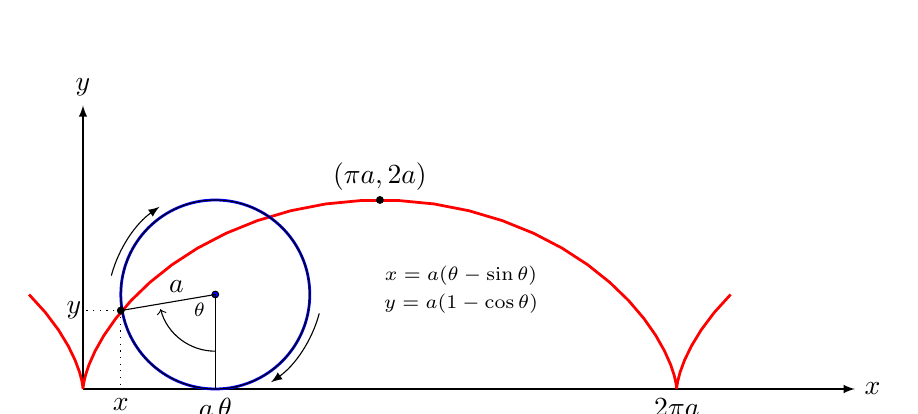
\begin{tikzpicture}[scale=1.2]
        \coordinate (O) at (0,0);
        \coordinate (A) at (0,3);
        \def\r{1} % radius
        \def\c{1.4} % center
        \coordinate (C) at (\c, \r);
      
      
        \draw[-latex] (O) -- (A) node[anchor=south] {$y$};
        \draw[-latex] (O) -- (2.6*pi,0) node[anchor=west] {$x$};
        \draw[red,domain=-0.5*pi:2.5*pi,samples=50, line width=1] 
             plot ({\x - sin(\x r)},{1 - cos(\x r)});
        \draw[blue, line width=1] (C) circle (\r);
        \draw[] (C) circle (\r);
      
        % coordinate x 
        \def\x{0.4} % coordinate x
        \def\y{0.83} % coordinate y
        \def\xa{0.3} % coordinate x for arc left
        \def\ya{1.2} % coordinate y for arc left
        \coordinate (X) at (\x, 0 );
        \coordinate (Y) at (0, \y );
        \coordinate (XY) at (\x, \y );
      
        \node[anchor=north] at (X) {$x$} ;
      
        % draw center of circle
        \draw[fill=blue] (C) circle (1pt);
      
        % draw radius of the circle
        \draw[] (C) -- node[anchor=south] {\; $a$} (XY);
      
        % bottom of circle, radius to the bottom
        \coordinate (B) at (\c, 0);
        \draw[] (C) -- (B) node[anchor=north] {$a \, \theta$};
      
        % projections of point XY
        \draw[dotted] (XY) -- (X);
        \draw[dotted] (XY) -- (Y) node[anchor=east, xshift=1mm] {$\quad y$};
      
        % arc theta
        % start arc
        \coordinate (S) at (\c, 0.4);
        \draw[->] (S) arc (-90:-165:0.6);
        \node[xshift=-2mm, yshift=-2mm] at (C) {\scriptsize $\theta$};
      
        % arc above
        \coordinate (AA) at (\xa, \ya);
        \draw[-latex, rotate=25] (AA) arc (-220:-260:1.3);
      
        % arc below
        \def\xb{2.5} % coordinate x for arc bottom
        \def\yb{0.8} % coordinate y for arc bottom
        \coordinate (AB) at (\xb, \yb);
        \draw[-latex, rotate=-10] (AB) arc (-5:-45:1.3);
      
      
      
        % XY dot
        \draw[fill=black] (XY) circle (1pt);
      
      
        % top label
        \coordinate (T) at (pi, 2);
        \node[anchor=south] at (T)  {$(\pi a, 2 a )$} ;
        \draw[fill=black] (T) circle (1pt);
      
        % equations
        \coordinate (E) at ( 4,1.2);
        \coordinate (F) at ( 4,0.9);
        \node[] at (E) {\scriptsize $x=a(\theta - \sin \theta)$};
        \node[] at (F) {\scriptsize $y=a(1 - \cos \theta)$};
      
        % label 2pi a
        \coordinate (TPA) at (2*pi, 0);
        \node[anchor=north] at (TPA) {$2 \pi a$};
      
      
    \end{tikzpicture}
    \caption{Graf cikloide iz zgleda \ref{zgl:9}.}
\end{figure}

%\begin{figure}[hbt!]
    
%    \caption{Skica cikloide iz zgleda \ref{zgl:9}.}
%\end{figure}

Vemo že, da lahko tangentno premico zapišemo kot
$\vec{\rho} = \vec{r} + \lambda \dvec{r} (t),\ \lambda \in \R$ oziroma 
$$\vec{\rho} = (x(t) + \lambda \dvec{x}(t), y(t) + \lambda \dvec{y}(t)).$$
V ravnini lahko zlahka poiščemo normalo na $\lambda$ v točki $\vec{r} (t)$.
Vektor $\vec{N} = (-\dot{y}, \dot{x})$ je pravokoten na vektor $\dvec{r} = (\dot{x}, \dot{y})$, saj je njun skalarni produkt enak $0$.
Torej je enačba normalne premice ne $\Gamma(t)$ v točki $\vec{r} (t)$ enaka
$$\vec{\rho_N} (\lambda) = \vec{r} (t) + \lambda \vec{N} (t) = (x(t)- \lambda \dot{y} (t), y(t) + \lambda \dot{x} (t)).$$

\begin{izrek}
    Naj bo $\vec{r}(t) = (\vec{x}(t), \vec{y} (t))$ zvezno odvedljiva pot v $\R^2$, $t \in I \subseteq \R$.
    Naj bo za $t_0 \in I$ odvod poti enak
    $\dvec{r}(t) = (\dot{x}(t), \dot{y}(t)) \neq \vec{0}.$
    Potem obstaja okolica $t_0 \in U \subseteq I$ točke $t_0$, da lahko množico $\vec{r} (U) \subseteq \R^2$ predstavimo ali kot graf neke funkcije $f(x)$ na $x$-osi ali kot graf neke $C^1$ funkcije $g(y)$ na $y$-osi.
    \begin{itemize}
        \item če je $\dot{x}(t_0) \neq 0$, je
        $\vec{r} (U) = \{(x, f(x)); x \in J_x\}$
        \item če je $\dot{y}(t_0) \neq 0$, je
        $\vec{r} (U) = \{(g(y), y); y \in J_y\}$
    \end{itemize}
\end{izrek}
\begin{opomba}
    Pri zgornjem izreku smo z $J_x$ in $J_y$ označili zaporedoma okolici $x(t_0)$ in $y(t_0)$.
\end{opomba}

\begin{dokaz}
    Naj bo $\dot{x} (t_0) \neq 0.$
    Denimo, da je $\dot{x} (t_0) > 0$.
    Potem je $\dot {x} (t)> 0$ v okolici $U$ točke $t_0$ v $I$ (to velja zato, ker je $x \in C^1 (I)$ in je odvod zvezen).
    Torej je $x$ na $U$ strogo naraščajoča in ima $X : U \rightarrow X(U) = J_x$ inverz $\tau : J_x \rightarrow U$, da je $\tau \in C^1 (J_x)$ in posledično $\tau '(x) = \frac{1}{\dot{x}(\tau(x))}$ zvezna na $J_x$.
    Sedaj definirajmo $f: J_x \rightarrow \R$ kot
    $f(x) = y(\tau(x)).$
    Potem je 
    \begin{equation*}
        \vec{r} = \{(x(t), y(t)); t \in U\} = \{(x, f(x)); x \in J_x\} \qedhere
    \end{equation*}
\end{dokaz}
\begin{zgled}
    Z implicitno enačbo $(x^2 + y^2)^2 = 2(x^2 - y^2)$ je podana krivulje lemniskate, ki ima parametrizacijo
    $$x(t) = \frac{\sqrt{2} \cos {t}}{1 + \sin^2 (t)}, \quad y(t) = \frac{\sqrt{2} \sin {t} \cos {t}}{1 + \sin^2 (t)}.$$
    Oglejmo si sedaj odvoda:
    \begin{itemize}
        \item $\dot{x} = \sqrt{2} \frac{(- \sin t) (2 + \cos^2 (t))}{(1 + \sin^2 (t))^2}, \quad \dot{x} = 0 \iff t = k \pi;\ k \in \Z$
        \item $\dot{y} = \sqrt{2} \frac{\cos^2 (t) - 2\sin^2 (t)}{(1 + \sin^2 (t))^2}, \quad \dot{y} = 0 \iff \tan^2 (t) = \frac{1}{2}$
    \end{itemize}
    Torej je $\vec{r} (t) \neq \vec{0}$ za vse $t$.
    Velja pa tudi $\vec{r} \left( \frac{\pi}{2}\right) = \vec{r} \left( \frac{3\pi}{2}\right) = (0,0)$, vendar pa $\dvec{r} \left(\frac{\pi}{2} \right) = \left(-\frac{\sqrt{2}}{2}, - \frac{\sqrt{2}}{2}\right)$ in $\dvec{r} \left(\frac{3 \pi}{2}\right) = \left(\frac{\sqrt{2}}{2}, \frac{\sqrt{2}}{2}\right)$.
    Torej lemniskata v $(0,0)$ seka samo sebe.
\end{zgled}

\begin{figure}[hbt!]
    \centering
    \begin{tikzpicture}
        \begin{axis}[
            ymin=-1, ymax=1,
            xmin=-2, xmax=2,
            ytick={0},
            xtick={-1,0,1},
            %ymajorgrids=true,
            %grid style=dashed,
        ]
        %\addplot[domain=0.0001:5] {x^(1/x)};
            \addplot[domain=-pi:pi, samples=50] ({((2)^(1/2) * cos(deg(x)))/(1 + sin(deg(x)) * sin(deg(x)))},{((2)^(1/2) * sin(deg(x)) * cos(deg(x)))/(1 + sin(deg(x)) * sin(deg(x)))});
            \addplot[domain=-2:2, color=gray, dashed] {0};
            \addplot[dashed, color=gray] coordinates {(0,-1)(0,1)};
        \end{axis}
    \end{tikzpicture}
    \caption{Graf lemniskate.}
\end{figure}
\clearpage
    \section{INTEGRAL}

\subsection{Nedoločeni integral}

Naj bo $I \subseteq \R$ interval in $f: I \rightarrow \R$ funkcija.

\begin{definicija}
    Funkcija $F: I \rightarrow \R$ je nedoločeni integral ali primitivna funkcija funkcije $f: I \rightarrow \R$, če je $F$ odvedljiva na $I$ in velja $F'(x) = f(x)$ za $\forall x \in I$.
\end{definicija}

\begin{zgled}
    Omenimo dva primera nedoločenega integrala.
    \begin{enumerate}
        \item Nedoločeni integral funkcije $f(x) = \cos x$ je $F(x) = \sin x$, saj je $F'(x) = (\sin x)' = \cos x$.
        \item Nedoločeni integral funkcije $f(x) = x^n,\ n \neq -1$ je $F(x) = \frac{1}{n+1} x^{n+1}$. 
        Če pa je $f(x) = \frac{1}{x}$, potem je $F(x) = \ln |x|$.
    \end{enumerate}
\end{zgled}

\begin{trditev}
    Naj bo $F(x)$ nedoločeni integral funkcije $f$ na intervalu $I \subseteq \R$.
    Potem je vsak nedoločeni integral funkcije $f$ na $I$ oblike $G(x) = F(x) + c;\ x \in I$ za neko konstanto $c \in \R$.
\end{trditev}

\begin{opomba}
    Množica $\{F + c; c \in \R\}$ je množica vseh nedoločenih integralov funkcije $f$ na $I$.
    Torej: če ima $f$ en nedoločeni integral, je množica vseh nedoločenih integralov enoparametrična ($\sim \R$).
\end{opomba}

\begin{dokaz}
    Če je $F$ nedoločeni integral funkcije $f$ na $I$, potem je očitno tudi $F + c,\ c \in \R$ nedoločeni integral sunkcije $f$ na $I$.
    Dokazati moramo, da je vsak nedoločeni integral $G$ funkcije $f$ na $I$ oblike $G(x) = F(x) + c$.
    Predpostavimo torej, da je $G$ nedoločeni integral $f$ na $I$. Potem velja $G' = f$ in $F' = f$ na $I$.
    Sedaj tvorimo funkcijo $H = G - F$.
    Potem za $\forall x \in I$ velja $H' = G' - F' = 0$, torej je $H' = 0$ na $I$.
    Zato je $H$ konstantna funkcija na $I$ in od tod sledi $G(x) = F(x) + c$.
\end{dokaz}

To označimo $\int f(x)\,dx = F(x) + c$, kjer je $F$ nek partikularen nedoločeni integral, $c \in \R$ pa poljubna konstanta.
To pomeni $$\int f(x)\,dx = \int dF_x = F(x) + c.$$
Od tod sledi, da je nedoločeni integral, če obstaja, nekkšna inverzna operacija od diferenciala $d$.
Obstoj nedoločeneg integrala pa ni samoumeven -- v splošnem ta ne obstaja.

\begin{zgled}
    Vzemimo funkcijo $$f(x) = \begin{cases}
        -1 ;& x < 0\\
        1 ;& x \geq 0
    \end{cases}$$
    Dokazali bomo, da ta funkcija nima nedeločenega integrala na $\R$.
    Predpostavimo nasprotno -- naj bo $F$ njen nedoločeni integral na $\R$.
    Potem mora biti za $x<0$ nedoločeni integral oblike $F(x) = - x + c_1$, za $x > 0$ pa $F(x) = x + c_2$.
    Ker je $F$ odvedljiva na $\R$ ($F' = f$), je $F$ zvezna na $\R$.
    Torej velja $$F(0) = \llimf{x}{0}{F(x)} = c_1 = \rlimf{x}{0}{F(x)} = c_2.$$
    Zato je $F(x) = |x| + c$ za nek $c \in \R$ in $F$ ni odvedljiva v $x = 0$, kar pa je protislovje.
\end{zgled}

\begin{opomba}
    Kasneje bomo dokazali, da ima vsaka zvezna funkcija na intervalu $I \subseteq \R$ nedoločeni integral.
    Zveznost je torej zadostni pogoj za obstoj nedoločenega integrala, ni pa potreben.
\end{opomba}

\begin{zgled}
    Primer: funkcija $$F(x) = \begin{cases}
        x^2 \sin \frac{1}{x} ;& x \neq 0\\
        0;& x = 0
    \end{cases}$$ je nedoločeni integral funkcije $$f(x) = F'(x) = \begin{cases}
        2x \sin \frac{1}{x} - \cos \frac{1}{x} ;& x \neq 0\\
        0;& x = 0
    \end{cases},$$ ta pa ni zvezna v točki $0$.
\end{zgled}
\begin{comment}
\subsection{Tabela osnovnih nedoločenih integralov}

\begin{table}[htb]
    \centering
    \begin{tabular}{cc}
        \toprule
        $f(x)$ & $\int f(x)\,dx$\\
        \midrule
        $x^n;\ n \neq -1$ & $\frac{1}{n+1} x^{n+1} + c$\\
        $\frac{1}{x}$ & $\ln |x| + c$\\
        $e^x$ & $e^x + c$\\
        $\sin x$ & $- \cos x + c$\\
        $\cos x$ & $\sin x + c$\\
        $\frac{1}{\cos^2 x}$ & $\tan x + c$\\
        $\frac{1}{\sin^2 x}$ & $- \cot x + c$\\
        $\frac{1}{1 + x^2}$ & $\arctan x + c$\\
        $\frac{1}{\sqrt{1-x^2}}$ & $\arcsin x + c$\\
        $\frac{1}{\sqrt{x^2 + a}}$ & $\ln (x + \sqrt{x^2 + a}) + c$\\
        \bottomrule
    \end{tabular}
\end{table}
\end{comment}
\subsection{Osnovna pravila za iskanje nedoločenih integralov}

Naslednja pravila izhajajo iz pravil za odvajanje.
Naj bosta $f,g$ funkciji, ki imata nedoločena integrala $F, G$.
Potem veljajo naslednje trditve.
\begin{itemize}
    \item Aditivnost: $\int (f+g)(x)\,dx = \int f(x)\,dx + \int g(x)\,dx$.
    \item Homogenost: $\int (\alpha f) (x)\,dx = \alpha \int f(x)\,dx$ za poljuben $\alpha \in \R$.
    \item Integracija per partes. Naj bosta $u,v$ odvedljivi na $I$. Potem velja
    $\int u v' = u v - \int u' v.$
\end{itemize}

    Razmislimo o vpeljavi nove spremenljivke v nedoločeni integral.
    Naj bo $\phi: J_t \rightarrow I$ odvedljiva, strogo monotona bijekcija z odvedljivim inverzom ($\phi'(t) \neq 0,\ \forall t$).
    Naj bo $G(t) = \int f(\phi (t)) \phi'(t)\,dt$. Potem velja:
    \begin{align*}
        F'(x) &= G'(\phi^{-1} (x)) (\phi^{-1})' (x)\\
        &= f(\phi (\phi^{-1} (x))) \cdot \phi'(\phi^{-1}(x)) \cdot (\phi^{-1})'(x)\\
        &= f(x) \cdot 1 = f(x).
    \end{align*} 
    in $F(x) = G(\phi^{-1} (x))$ je nedoločeni integral $f$.

\begin{opomba}
    Točki (1) in (2) izhajata iz linearnosti odvoda, točka (3) izhaja iz Leibnizovega pravila odvajanja in točka (4) izhaja iz verižnega pravila o odvajanju.
    Zadnji razmislek pa nam pove, da z ustrezno substitucijo $x = \phi(t),\ dx = \phi'(t)\,dt$ dobimo $\int f(x)\,dx = \int f(\phi(t)) \phi'(t)\,dt$.
\end{opomba}

\begin{zgled}
    Oglejmo si primera odvajanja per partes in z uvedbo nove spremenljivke:
    \begin{itemize}
        \item $\int \ln x\,dx = x \ln x - \int x \cdot \frac{1}{x}\,dx = x \ln x - x + c$
        \item $\int x e^{x^2}\,dx = \int \sqrt{t} e^t \frac{1}{2 \sqrt{t}}\,dt = \frac{1}{2} \int e^t\,dt = \frac{1}{2} e^t\,dt + c= \frac{1}{2}e^{x^2} + c$
    \end{itemize}
\end{zgled}

\begin{opomba}
    Hitro naletimo na elementarne funkcije, katerih nedoločeni integral ne moremo izraziti z elementarnimi funkcijami.
    Primer takega integrala je $\int e^{x^2}\,dx$.
\end{opomba}

Razred funkcij, ki ga bomo posebej obravnavali, so racionalne funkcije, saj imajo elementarne nedoločene integrale.
To je seveda očitno za polinome. Pri funkcijah oblike $f(x) = \frac{p(x)}{q(x)}$, kjer sta $p,q$ realna polinoma, pa se moramo nekoliko bolj potruditi.
Najprej delimo $p$ s $q$, da pridemo do primera $st\ p < st\ q$, nato pa $q$ razcepimo na linearne in kvadratne nerazcepne (nad $\R$) faktorje.
Tako lahko $f = \frac{p}{q}$ zapišemo kot vsoto parcialnih ulomkov oblike
$$\frac{A}{(x - \alpha)^m} \quad \text{in} \quad \frac{Ax + B}{(x^2 + ax + b)^m}.$$
Integrali sumandov 1. oblike so znani:
$$\int \frac{A}{(x - \alpha)^m}\,dx = \begin{cases}
    A \ln |x - \alpha| + c ;& m = 1\\
    - \frac{A}{(m + 1)(x - \alpha)^{m - 1}} ;& m > 1
\end{cases},$$
integrali sumandov 2. oblike pa so:
\begin{itemize}
    \item $E \ln (x^2 + ax + b) + F \arctan \left(\frac{2x + a}{\sqrt{4b - a^2}} \right)$ za $m = 1$ in 
    \item $\frac{r(x)}{(x^2 + ax + b)^{m-1}} + F \arctan \frac{2x + a}{\sqrt{4b - a^2}}$ za $m > 1$.
\end{itemize}
Pri tem sta $E,F$ konstanti, $r(x)$ pa polinom stopnje $2m -3$. Te podatke dobimo z odvajanjem obeh strani enačbe in reševanjem dobljenega sistema linearnih enačb.

\begin{zgled}
    Obravnavajmo dva primera integralov racionalnih funkcij.
    \begin{itemize}
        \item $\int \frac{x + 1}{x^2 + 1}\,dx = \frac{1}{2} \ln (x^2 + 1) + \arctan x + c$
        \item $\int \frac{dx}{(x^2 + 1)^2} = \frac{Ax + B}{x^2 + 1} + D \arctan x + c$, odvajamo in dobimo $A=D= \frac{1}{2},\ B = 0.$
    \end{itemize}
\end{zgled}

\begin{opomba}
    Integral sode funkcije je liha funkcija (do konstante $c$ natančno) in obratno.
\end{opomba}

\subsection{Določeni integral}

Nedoločeni integral, če obstaja, je taka funkcija $F: [a, b] \rightarrow \R$, da je $F'(x) = f(x),\ \forall x \in [a, b]$.
Določeni integral, če obstaja pa je število $\int_{a} ^{b} f(x)\,dx \in \R$.
Motivacija za uvedbo določenega integrala je izračun ploščine lika pod grafom funkcije $f: [a, b] \rightarrow (0, \infty)$, ki leži nad intervalom $[a, b]$.
Fizikalna interpretacija tega je naslednja: če je $x = t$ čas in $f(x) = v(t)$ hitrost, je $\int_{0} ^{T} v(t)\,dt$ pot, opravljena v času od $0$ do $T$.

\begin{opomba}
    Če bo $f$ predznačena, bo $\int_{a} ^a f(x)\,dx$ razlika ploščin nad $x$-osjo in pod $x$-osjo.
    Z drugimi besedami, določeni integral izračuna "`predznačeno ploščino oz. signed area under a graph"'.
\end{opomba}

Pri definiranju določenega integrala si bomo ogledali dva ekvivalentna pristopa: Darbouxjeve in Riemannove vsote.
Naj bo $[a, b]$ končen zaprt interval na $\R$ in $a < b$.
Delitev $D$ intervala $[a, b]$ je izbor končno mnogo točk
$$a = x_0 < x_1 < \dots < x_{n-1} < x_n = b,$$
kjer je $n$ poljubno naravno število. Sedaj definiramo še množico
$$\mathcal{T} = \{t_1, \dots, t_n;\ t_j \in [x_{j-1}, x_{j}]\},$$
kjer je $[x_{j-1}, x_j]$ podinterval delitve $D$.
Riemannova vsota, prirejena funkciji $f$, delitvi $D$ in izboru točk $\mathcal{T}$ je
$$R(f, D, \mathcal{T}) = \sum_{j = 1} ^n f(t_j) (x_j - x_{j-1}) = \sum_{j = 1} ^n f(t_j) \Delta x_j.$$
To je vsota ploščin pravokotnikov z osnovo $\Delta x_j$ in višino $f(t_j)$, s čimer aproksimiramo ploščino lika pod grafom funkcije $f(x)$.

\begin{definicija}
    Naj bo $f:[a,b] \rightarrow \R$. Funkcija $f$ je Riemannovo integrabilna na $[a, b]$, če za vsak $\varepsilon > 0$ obstaja tak $\delta > 0$, da za vsako delitev $D = \{x_0 < x_1 < \dots < x_n\}$ intervala $[a, b]$, ki zadošča pogoju $\Delta x_j < \delta,\ \forall j = 1, \dots, n$, 
    in za poljuben izbor točk $$\mathcal{T} = \{t_1, \dots, t_n;\ t_j \in [x_{j-1}, x_j],\ j = 1, \dots, n\}$$
    velja $|R(f, D, \mathcal{T}) - I| < \varepsilon$.
    To lahko zapišemo kot $$\limf{\max_j \Delta x_j}{0}{R(f, D, \mathcal{T})} = I = \int_{a} ^b f(x)\,dx.$$
\end{definicija}

\begin{opomba}
    Včasih se pri definiciji Riemannovih vsot poudari omejenost funkcije $f$, vendar pa se izkaže, da iz Riemannove integrabilnosti sledi omejenost na intervalu $[a, b].$
    Če $f$ ne bi bla omejena (denimo navzgor), potem obstaja zaporedje $(a_k)_{k = 1} ^{\infty},\ a_k \in [a, b]$, da je $f(a_k) > k,\ \forall k \in \N$.
    Brez škode za splošnost predpostavimo, da $(a_k)_{k = 1} ^{\infty}$ konvergira k $\alpha \in [a, b]$.
    Za dani $\varepsilon$ si izberemo $\delta > 0$ in delitev $D$ intervala $[a, b]$, ki ali vsebuje $\alpha$ v notranjosti enega od intervalov $[x_{j-1}, x_j]$ ali pa je $\alpha$ eno izmed krajišč $a, b$.
    Potem obstaja tak $k_0$, da za vsak $k \geq k_0$ velja, da $a_k$ leži v istem podintervalu kot $\alpha$: $[x_{j_0 -1}, x_{j_0}]$.
    Sedaj pa točke $t_1, \dots, t_{j_0 - 1}, t_{j_0 + 1}, \dots, t_{n}$ fiksiramo, točko $t_{j_0}$ pa izbiramo kot $a_k$. 
    Velja, da gredo tako dobljene Riemannove vsote preko vsake meje in ne konvergirajo k nekemu $I$.
\end{opomba}

\begin{zgled}
    Vzemimo funkcijo $$f(x) = \begin{cases}
        1 ;& x \geq 0\\
        -1 ;& x < 0
    \end{cases}$$ in $a < 0 < b.$ 
    Naj bo $D = \{x_0 < \dots < x_n\}$ delitev $[a, b]$ in naj bodo
    $$x_0 < x_1 < \dots < x_{i_0} < 0 \leq x_{i_0 +1} < \dots < x_n.$$
    Določimo še množico točk $\mathcal{T} = \{t_j;\ j = 1, \dots, n,\ t_j \in [x_{j-1} - x_j]\}$.
    Potem je 
    \begin{align*}
        R(f, D, \mathcal{T}) = \sum_1 ^n f(t_j) \Delta x_j
        &= \sum_1 ^{i_0} f(t_j) \Delta x_j + f(t_{i_0 +1}) \Delta x_{i_0 + 1} + \sum_{i_0 + 2} ^n f(t_j) \Delta x_j\\
        &= (-1) (x_{i_0} - a) + f(t_{i_0 + 1}) \Delta x_{i_0 + 1} + (b - x_{i_0 + 1})\\
        &= a+b -x_{i_0} - x_{i_0 + 1} + f(t_{t_0 + 1}) (x_{i_0 + 1} - x_{i_0})\\
        &= \begin{cases}
            a+ b - 2 x_{i_0} ;& f(t_{i_0 + 1}) = 1\\
            a +b - 2 x_{i_0 + 1} ;& f(t_{i_0 + 1}) = -1
        \end{cases}.
    \end{align*}
    Trdimo, da je $I = \int_a ^b f(x)\,dx = a + b$.
    Naj bo $\varepsilon > 0$. Naj bo $\max \Delta x_j < \delta = \frac{\varepsilon}{2}$.
    Potem je $x_{i_0} < 0 < x_{i_0 + 1}$ in $x_{i_0 +1} - x_{i_0} < \delta = \frac{\varepsilon}{2}$ in od tod sledi $|x_{i_0 + 1}| < \frac{\varepsilon}{2}$ in $|x_{i_0}| < \frac{\varepsilon}{2}$.
    Od tod pa sledi $$|R(f, D, \mathcal{T}) - (a+b)| = \begin{cases}
        |2 x_{i_0}| < \varepsilon\\
        |2 x_{i_0 + 1}| < \varepsilon
    \end{cases}$$ in smo dokazali.
\end{zgled}

\begin{zgled}
    Naj bo funkcija $$f(x) = \begin{cases}
        1 ;& x \in \Q\\
        0;& x \notin \Q\\
    \end{cases}.$$ Potem za vsak $a < b$ integral $\int_a ^b f(x)\,dx$ ne obstaja.
    Naj bo $D$ delitev $a = x_0 < x_1 < \dots < x_n = b$.
    Če za $\mathcal{T}$ izbiramo racionalne točke $t_j \in [x_{j-1}, x_j]$, dobimo $R(f, D, \mathcal{T}) = (b-a)$, 
    če pa za $\mathcal{T}$ izbiramo iracionalne točke $t'_j$, dobimo $R(f, D, \mathcal{T}) = 0.$
    To pomeni, da ne obstaja tak $I$, da velja $\limf{\max \Delta x_j}{0}{R(f, D, \mathcal{T})} = I.$
\end{zgled}

Drugi pristop k določenemu intervalu so Darbouxjeve vsote.
Naj bo $f: [a, b] \rightarrow \R$ omejena in naj bo $D = \{x_0 = a < \dots < x_n = b\}$ delitev $[a, b]$.
Naj bo $m = \inf_{[a,b]} f(x)$ in $M = \sup_{[a,b]} f(x)$.
Označimo $m_j = \inf_{[x_{j-1}, x_j]} f(x)$ in $M_j = \sup_{[x_{j-1}, x_j]} f(x)$ za $j = 1, \dots, n$.
Očitno velja $m \leq m_j \leq M_j \leq M$ za vsak $j = 1, \dots, n$.
Sedaj definiramo:
\begin{itemize}
    \item spodnja Darbouxjeva vsota za delitev $D$ je
    $s(f, D) = \sum_1 ^n m_j \Delta x_j = s(D),$
    \item zgornja Darbouxjeva vsota za delitev $D$ je
    $S(f, D) = \sum_1 ^n M_j \Delta x_j = S(D).$
\end{itemize}
Na liku, ki ga oklepa graf funkcije $f$ z $x$-osjo, $s(D)$ aproksimira ploščino včrtanih pravokotnikov, $S(D)$ pa ploščino očrtanih pravokotnikov.
Očitno velja:
\begin{itemize}
    \item $m(b - a) \leq s(D) \leq S(D) \leq M(b-a)$
    \item $s(D) \leq R(f, D, \mathcal{T}) \leq S(D)$ za poljubne točke $\mathcal{T}$.
\end{itemize}

\begin{definicija}
    Delitev $D'$ je nadaljevanje delitve $D$ intervala $[a, b]$, če je $D \subseteq D'$.
    To pomeni, da je vsaka delilna točka $D$ tudi delilna točka $D'$, $D'$ pa lahko vsebuje tudi dodatne delilne točke.
    Pogosto rečemo, da je $D'$ finejša kot delitev $D$.
\end{definicija}

\begin{trditev}
    Če je $D \subseteq D'$, je $$s(D) \leq s(D') \leq S(D') \leq S(D).$$
\end{trditev}

\begin{dokaz}
    Dovolj je preveriti primer $D' = D \cup \{x'\}$, saj trditev v splošnem sledi s končno indukcijo.
    Naj bo $D = \{x_0 < x_1 < \dots < x_n\}$ in $x' \in (x_{j-1} , x_j)$ za nek $j$.
    Potem velja $m_j \leq \inf_{[x_{j-1}, x']} f(x) = m'_j$ in $m_j \leq \inf_{[x', x_{j+1}]} f(x) = m''_j.$
    Podobno velja tudi $M'_j \leq M_j$ in $M''_j \leq M_j$.
    Torej velja
    \begin{align*}
        m_j \Delta x_j &= m_j (x_j - x_{j-1})\\
        &= m_j ((x_j - x') + (x' - x_{j-1}))\\
        &= m_j (x_j - x') + m_j (x' - x_{j-1})\\
        &\leq m''_j (x_j - x') + m'_j (x' - x_{j-1})
    \end{align*}
    Na ostalih intervalih ni sprememb, torej je res $s(D) \leq s(D')$ in podobno za zgornje vsote $S(D') \leq S(D)$.
\end{dokaz}

\begin{trditev}
    Naj bosta $D_1, D_2$ delitvi $[a, b]$. Potem je $s(D_1) \leq S(D_2)$.
\end{trditev}

\begin{dokaz}
    Naj bo $D = D_1 \cup D_2$. Potem je $D$ nadaljevanje delitev $D_1$ in $D_2$. Torej:
    \begin{equation*}
        s(D_1) \leq s(D) \leq S(D) \leq S(D_2). \qedhere
    \end{equation*}
\end{dokaz}

Naj bo $S = \inf_D S(D)$ zgornji Darbouxjev integral in $s = \sup_D s(D)$ spodnji Darbouxjev integral.
Očitno velja $$m (b-a) \leq s \leq S \leq M(b-a).$$
\begin{definicija}
    Funkcija $f: [a, b] \rightarrow \R$ je integrabilna v smislu Darboux-ja, če je $S = s$.
    To število je Darbouxjev integral funkcije $f$ na $[a, b].$
\end{definicija}

\begin{trditev}
    Omejena funkcija $f: [a, b] \rightarrow \R$ je po Darbouxju integrabilna natanko tedaj, ko za $\forall \varepsilon > 0$ obstaja delitev $D$ intervala $[a, b]$, da je $S(D) - s(D) < \varepsilon.$
\end{trditev}

\begin{dokaz}
    Za vsako delitev $D$ velja $s(D) \leq s \leq S \leq S(D)$. Torej če je izpolnjen epsilonski pogoj, mora biti $s = S$ in $f$ je po Darbouxju integrabilna.
    Pokazati moramo še obratno trditev: denimo, da je $s = S$ in vzemimo poljuben $\varepsilon$.
    Ker je $s = \sup_D s(D)$, obstaja delitev $D_1$, da je 
    $$s - \frac{\varepsilon}{2} < s(D_1) \leq s.$$ Podobno obstaja delitev $D_2$, da je 
    $$S \leq S(D_2) < S + \frac{\varepsilon}{2}.$$ Sedaj izberemo $D = D_1 \cup D_2$. Potem je 
    $$s - \frac{\varepsilon}{2} < s(D_1) \leq s(D) \leq S(D) \leq S(D_2) < S + \frac{\varepsilon}{2}$$ in zato $S(D) - s(D) < \varepsilon$.
\end{dokaz}

\begin{izrek}
    Omejena funkcija $f: [a, b] \rightarrow \R$ je Riemannovo integrabilna natanko tedaj, ko je integrabilna po Darbouxju.
    V tem primeru se njen Riemannov integral ujema z njenim Darbouxjevim integralom.
\end{izrek}

\begin{dokaz}
    ($\Rightarrow$) Naj bo $f$ Riemannovo integrabilna na $[a, b]$. Naj bo $I_R$ njen Riemannov integral.
    Potem za $\forall \varepsilon > 0$ obstaja tak $\delta > 0$, da je $|R(f, D, \mathcal{T}) - I_R| < \frac{\varepsilon}{3}$ za vsako delitev $D$ s pogojem $\max_j \Delta x_j < \delta$ in za vsak izbor točk $\mathcal{T}$.
    Naj bo $D$ delitev, ki zadošča temu pogoju.
    Če izbiramo točke $t_j \in [x_{j-1} , x_j]$ tako, da je $f(t_j)$ poljubno blizu $M_j = \sup_{[x_{j-1}, x_j]}$, bo $R(f, D, \mathcal{T})$ poljubno blizu $S(D)$, torej $|S(D) - I_R| \leq \frac{\varepsilon}{3}$.
    Podobno dobimo $|s(D) - I_R| \leq \frac{\varepsilon}{3}$ in od tod sledi $S(D) - s(D) \leq \frac{2 \varepsilon}{3} < \varepsilon$.
    Od tod pa sledi, da je $f$ integrabilna po Darbouxju. Ker je za vsako delitev $D$
    $s(D) \leq R(f, D, \mathcal{T}) \leq S(D)$, sledi, da je $I_R$ tudi Darbouxjev integral.

    ($\Leftarrow$) Naj bo $f$ po Darbouxju integrabilna. Naj bo $\varepsilon > 0.$
    Obstaja delitev $D_0$, da velja $S(D_0) - s(D_0) < \frac{\varepsilon}{2}$.
    \begin{lema}
        Naj bo $D_0$ delitev $[a, b].$ Potem obstaja tak $\delta > 0$, da je za vsako delitev, za katero je $\max_j \Delta x_j < \delta,$ vsota dolžin delilnih intervalov, ki niso vsebovani v nobenem od delilnih intervalov $D_0$, pod $\varepsilon$.
    \end{lema}
        Sedaj za '$\varepsilon$' v pomožni trditvi uporabimo $\frac{\varepsilon}{2(M - m)}$ in uporabimo ustrezen $\delta > 0$.
        Naj bo $D$ poljubna delitv, da je $\max_{j} \Delta x_j < \delta.$ Sedaj zapišemo
        \begin{align*}
            S(D) - s(D) &= \sum_j M_j \Delta x_j - \sum _j m_j \Delta x_j\\
            &= \sum_j (M_j - m_j) \Delta x_j\\
            &= \sum ' (M_j - m_j) \Delta x_j + \sum '' (M_j - m_j) \Delta_j\\
            &\leq S(D_0) - s(D_0) + (M - m) \sum '' \Delta x_j\\
            &< \frac{\varepsilon}{2} + (M-m) \frac{\varepsilon}{2(M-m)} = \varepsilon.
        \end{align*}
        Pri tem smo vsoto delilnih intervalov $D$, ki so bili vsebovani v enam izmed delilnih intervalov $D_0$, označili z $\sum'$, preostale intervale pa smo seštevali po $\sum''$.
        Sedaj smo našli tak $\delta > 0$, da za $\max \Delta x_j < \delta$ velja $S(D) - s(D) < \varepsilon.$
        Ker je $s(D) \leq I_D \leq S(D)$ in $s(D) \leq R(f, D, \mathcal{T}) \leq S(D)$, velja $|R(f, D, \mathcal{T}) - I_D| < \varepsilon$ in $f$ je po Riemannu integrabilna.
\end{dokaz}

\begin{dokaz}[Dokaz leme]
    Vzemimo delitev $D_0 = \{a = x_0 ^{(0)} < x_1 ^{(0)} < \dots < x_n ^{(0)} = b\}$ delitev intervala $[a, b]$.
    Sedaj definirajmo $\delta = \frac{\varepsilon}{n - 1}$.
    Naj bo $D$ delitev intervala $[a, b]$, da je $\max_j \Delta_j < \delta$.
    Intervalov delitve $D$, ki vsebujejo v notranjosti katero izmed točk $x_1 ^{(0)}, \dots, x_{n-1} ^{(0)}$, je največ $n - 1$ in njihova skupna dolžina je manj kot $(n-1) \delta = \varepsilon$.
\end{dokaz}

\begin{izrek}
    Vsaka zvezna funkcija $f: [a, b] \rightarrow \R$ je integrabilna na $[a, b].$
\end{izrek}

\begin{dokaz}
    Naj bo $\varepsilon > 0$. Ker je $f$ zvezna na $[a, b]$, je na $[a, b]$ enakomerno zvezna in obstaja tak $\delta > 0$, da za vsaka $x', x'' \in [a, b]$ velja
    $$|x' - x''| < \delta \implies |f(x') - f(x'')| < \frac{\varepsilon}{b-a}.$$
    Naj bo $D$ delitev, da je $\max_j \Delta x_j < \delta.$
    Potem je za vsak $j$:
    $$M_j - m_j = \max_{[x_{j-1}, x_j]} f(x) - \min_{[x_{j-1}, x_j]} f(x) < \frac{\varepsilon}{b-a}.$$
    Od tod pa sledi 
    $$S(D) - s(D) = \sum_j (M_j- m_j) \Delta x_j < \frac{\varepsilon}{b-a} \sum_j \Delta x_j = \varepsilon$$
    in $f$ je integrabilna.
\end{dokaz}

\begin{izrek}
    Naj bo $f:[a, b] \rightarrow \R$ monotona. Potem je $f$ integrabilna na $[a, b]$.
\end{izrek}

\begin{dokaz}
    Naj bo $\varepsilon > 0$. Naj bo $f$ naraščajoča in $D$ delitev $[a, b]$.
    Potem je $M_j = f(x_j)$ in $m_j = f(x_{j-1})$.
    Naj bo $\max_j \Delta x_j < \delta = \frac{\varepsilon}{f(b) - f(a)}$
    Zato je \begin{align*}
        S(D)- s(D) &= \sum_j (M_j - m_j) \Delta x_j\\
        &= \sum_j (f(x_j) - f(x_{j-1})) \Delta x_j\\
        &< \delta \sum_j (f(x_j) - f(x_{j-1}))\\
        &= \frac{\varepsilon}{f(b)- f(a)} (f(a) - f(b)) = \varepsilon
    \end{align*}
    in $f$ je integrabilna.
\end{dokaz}

\begin{opomba}
    Monotona funkcija $f$ ima na zaprtem intervalu $[a, b]$ števno mnogo skokov oziroma točk nezveznosti.
\end{opomba}

\begin{trditev}
    Naj bo $f: [a, b] \rightarrow \R$ omejena in zvezna na $(a, b)$.
    Potem je $f$ integrabilna na $f$.
\end{trditev}

\begin{dokaz}
    Naj bo $m = \inf_{[a,b]} f(x)$ in $M = \sup_{[a, b]} f(x)$.
    Če je $M = m$, je trditev očitna. Naj bo torej $m < M$ in $\varepsilon > 0$.
    Naj bosta $a' = a + \frac{\varepsilon}{3(M-m)}$ in $b' = b - \frac{\varepsilon}{3(M-m)}$.
    Če je potrebno, $\varepsilon$ zmanjšamo, da je $a < a' < b'< b$.
    Na $[a', b']$ je $f$ enakomerno zvezna in najdemo delitev $D'$, da je $S(D') - s(D') < \frac{\varepsilon}{3}$.
    Sedaj definiramo $D = D' \cup \{a, b\}$ in dobimo
    \begin{align*}
        S(D) - s(D) &= S(D') - s(D') + (M_1 - m_1) \Delta x_1 + (M_n -m_n) \Delta x_n\\
        &< \frac{\varepsilon}{3} + (M - m) \frac{\varepsilon}{3(M-m)} + (M - m) \frac{\varepsilon}{3(M- m)} = \varepsilon \qedhere
    \end{align*}
\end{dokaz}

\begin{izrek}
    Naj bo $f: [a, b] \rightarrow \R$ omejena funkcija. Naj bo $c \in (a, b)$.
    Potem je $f$ integrabilna na $[a, b]$ natanko tedaj, ko je integrabilna na $[a, c]$ in $[c,b]$.
    V tem primeru velja $$\int_a ^b f(x)\,dx = \int_a ^c f(x)\,dx + \int_c ^b f(x)\,dx.$$
\end{izrek}

\begin{dokaz}
    ($\Rightarrow$) Naj bo $f$ integrabilna na $[a, b]$ in naj bo $D$ delitev $[a, b]$, da je $S(D) - s(D) < \varepsilon$.
    Brez škode za  splošnost predpostavimo, da je $c$ v tej delitvi (sicer bi lahko vzeli njeno nadaljevanje).
    Naj bo $D = \{x_0 < x_1 < \dots < x_k = c < x_{k+1} < \dots < x_n\}$ in naj bo
    $D' = \{x_0 < x_1 < \dots < x_k\}$ delitev $[a, c]$ ter $D'' = \{x_k < \dots < x_n\}$ delitev $[c, b]$
    Sedaj pa velja $$S(D') - s(D') + S(D'') - s(D'') = S(D) - s(D) < \varepsilon$$ in od tod $S(D') - s(D') < \varepsilon$ ter $S(D'') - s(D'') < \varepsilon$,
    torej je $f$ integrabilna na $[a, c]$ in $[c, b]$.

    ($\Leftarrow$) Naj bo $f$ integrabilna na intervalih $[a, c]$ in $[c, b]$ in
    naj bo $\varepsilon > 0$. Obstaja delitev $D'$ intervala $[a, c]$ in $D''$ intervala $[c, b]$, da velja 
    $S(D') - s(D') < \frac{\varepsilon}{2}$ in $S(D'') - s(D'') < \frac{\varepsilon}{2}$.
    Naj bo $D = D' \cup D''$. Potem je $$S(D) - s(D) = S(D') - s(D') + S(D'') - s(D'') < \varepsilon$$
    in $f$ je integrabilna na $[a, b]$. Izraz $$\int_a ^b f(x)\,dx = \int_a ^c f(x)\,dx + \int_c ^b f(x)\,dx$$ pa dobimo z limitiranjem Riemannovih vsot z delitvami $D$, ki vsebujejo $c$ kot delilno točko:
    \begin{equation*}
        R(f, D, \mathcal{T}) = R(f, D', \mathcal{T}') + R(f, D'', \mathcal{T}'') \qedhere
    \end{equation*}
\end{dokaz}

\begin{definicija}
    Če je $f$ integrabilna na intervalu $[a, b]$, definiramo $\int_b ^a f(x)\,dx = - \int_a ^b f(x)\,dx$.
\end{definicija}

\begin{posledica}
    Naj bodo $a,b,c \in \R$ in $f$ integrabilna na največjem od zaprtih intervalov s krajišči v točkah $a, b, c$.
    Tedaj velja $$\int_a ^b f(x)\,dx = \int_a ^c f(x)\,dx + \int_b ^c f(x)\,dx.$$
\end{posledica}

\begin{posledica}
    Naj bo $F : [a, b] \rightarrow \R$ omejena in naj obstajajo točke $$a = c_0 < c_1 < \dots < c_m = b,$$ da je $f$ zvezna na $(c_{j-1}, c_j)$ za $\forall j$.
    Potem je $f$ integrabilna na $[a, b]$.
\end{posledica}

\begin{trditev}
    Naj bosta $f, g$ integrabilni na $[a, b]$. Tedaj so integrabilne funkcije $f+g, f-g, c f, |f|$.
    Pri tem velja:
    \begin{itemize}
        \item $\int_a ^b (f + g)(x)\,dx = \int_a ^b f(x)\,dx + \int_a ^b g(x)\,dx$
        \item $\int_a ^b (cf)(x)\,dx = c\int_a ^b f(x)\,dx$
        \item $\left|\int_a ^b f(x)\,dx\right| \leq \int_a ^b |f(x)|\,dx$
    \end{itemize}
\end{trditev}

\begin{opomba}
    Iz prve in druge točke izhaja, da je določeni integral linearen funkcional na vektorskem prostoru integrabilnih funkcij na $[a, b]$ (nad $\R$).
    Tretja točka pa je integralska različica trikotniške neenakosti.
\end{opomba}

\begin{dokaz}
    Prvi dve točki sledita direktno iz Riemannovih vsot. Dokažimo tretjo točko.
    Naj bo $D$ delitev $[a, b]$. Naj bo $\overline{M}_j = \sup_{[x_{j-1}, x_{j}]} |f|$ in $\overline{m}_j = \inf_{[x_{j-1}, x_{j}]} |f|$.
    Sedaj za vsaka $x, x' \in [x_{j-1}, x_j]$ velja trikotniška neenakost
    $$||f(x)| - |f(x')|| \leq |f(x) - f(x')| \leq M_j - m_j.$$
    Od tod sledi $\overline{M}_j - \overline{m}_j \leq M_j - m_j$.
    Torej je $$S(|f|, D) - s(|f|, D) \leq S(f, D) - s(f, D)$$
    in $|f|$ je integrabilna na $[a, b]$.
    Neenakost sledi iz Riemannovih vsot $|R(f, D, \mathcal{T})| \leq R(|f|, D, \mathcal{T})$.   
\end{dokaz}

\begin{trditev}
    Če sta $f$ in $g$ integrabilni na $[a, b]$ in je $f(x) \leq g(x)$ za $\forall x \in [a, b]$, potem je 
    $$\int_a ^b f(x)\,dx \leq \int_a ^b g(x)\,dx.$$
\end{trditev}

\begin{dokaz}
    Direktno sledi iz Riemannovih vsot: $R(f, D, \mathcal{T}) \leq R(f, D, \mathcal{T}).$
\end{dokaz}

\begin{posledica}
    Naj bo $f$ integrabilna na $[a, b]$ in naj bosta $m = \inf_{[a, b]} f$ ter $M = \sup_{[a, b]} f$.
    Potem je $$m (b-a) \leq \int_a ^b f(x)\,dx \leq M(b-a)$$ in vrednost $\frac{1}{b - a} \int_a ^b f(x)\,dx$ imenujemo povprečna vrednost $f$ na $[a, b]$.
\end{posledica}

\begin{posledica}
    Naj bo $f$ zvezna na $[a, b]$. Potem obstaja tak $c \in [a, b]$, da je $f(c) = \frac{1}{b-a} \int_a ^b f(x)\,dx.$
\end{posledica}

\subsection{Osnovni izrek integralskega računa}

\begin{izrek}[Newton-Leibnizov izrek]
    Naj bo $f: [a, b] \rightarrow \R$ integrabilna funkcija, ki ima nedoločeni integral na $[a, b]$:
    $F: [a, b] \rightarrow \R,\ F' = f$. Tedaj velja Newton-Leibnizova formula
    $$\int_a ^b f(x)\,dx = F(b) - F(a) = F(x) \Big|_a ^b.$$
\end{izrek}

\begin{dokaz}
    Naj bo $D = \{x_0 = a < x_1 < \dots < x_n = b\}$ delitev integrala $[a, b]$.
    Potem z uporabo Lagrangevega izreka in ustrezno izbiro točk $\mathcal{T} = \{t_1, t_2, \dots, t_n\}$ dobimo
    \begin{align*}
        F(b) - F(a) &= F(x_n) - F(x_{n-1}) + F(x_{n-1}) - F(x_{n-2}) + \dots + F(x_1) - F(x_0)\\
        &= F'(t_n) \Delta x_n + F'(t_{n-1}) \Delta x_{n-1} + \dots + F'(t_1) \Delta_1\\
        &= f(t_n) \Delta x_n + f(t_{n-1}) \Delta x_{n-1} + \dots + f(t_1) \Delta_1 = R(f, D, \mathcal{T}).
    \end{align*}
    Ker je $\limf{\max \Delta x_j}{\infty}{R(f, D, \mathcal{T})} = \int_a ^b f(x)\,dx$, mora veljati $\int_a ^b f(x)\,dx = F(b) - F(a)$.
\end{dokaz}

\begin{zgled}
    Oglejmo si funkcijo $$f(x) = \begin{cases}
        1; & x \geq 0\\
        0; & x < 0
    \end{cases}$$ na intervalu $[-3, 2]$.
    Vemo, da je ta funkcija integrabilna, nima pa nedoločenega integrala.
    Določeni integral funkcije $f(x)$ na $[-3, 2]$ je $$\int_{-3} ^2 f(x)\,dx = \int_{-3} ^0 f(x)\,dx + \int_0 ^2 f(x)\,dx = -3 + 2 = -1.$$
\end{zgled}

Pri katerih pogojih ima $f$ zagotovo nedoločeni integral? Oglejmo si funkcijo $F(x) = \int_a ^x f(t)\,dt$ -- integral kot funkcija zgornje meje.
\begin{izrek}
    Naj bo $f: [a, b] \rightarrow \R$ integrabilna. Potem je funkcija $F(x) = \int_a ^x f(t)\,dt$ zvezna na $[a, b]$.
    Če je $f$ v točki $x \in [a, b]$ zvezna, je $F$ v $x$ odvedljiva in velja $F'(x) = f(x).$
\end{izrek}

\begin{dokaz}
    Vemo, da je $f$ omejena na $[a, b].$ Potem obstaja $M \geq 0$, da je $|f(x)| \leq M$ za $\forall x \in [a, b]$.
    Naj bo $x \in [a, b].$ Potem je 
    \begin{align*}
        \left| F(x+h) - F(x) \right| &= \left| \int_x ^{x+h} f(t)\,dt \right|\\
        &\leq \left| \int_x ^{x+h} |f(t)|\,dt \right|\\
        &\leq M \left| \int_x ^{x+h} 1 \cdot\,dt \right| = M |h|,
    \end{align*}
    torej je $F$ zvezna v $x$, saj vzamemo $\delta = \frac{\varepsilon}{M}$ (če je $M = 0$, je trditev očitna).
    Naj bo sedaj $f$ zvezna v $x$ in $h \neq 0$. Potem je 
    \begin{align*}
        \frac{F(x+h) - F(x)}{h} &= \frac{1}{h} \int_{x} ^{x+h} f(t)\,dt\\
        &= \frac{1}{h} \int_{x} ^{x+h} (f(x) + (f(t) - f(x)))\,dt\\
        &= f(x) + \frac{1}{h} \int_{x} ^{x+h} (f(t) - f(x))\,dt.
    \end{align*}
    Naj bo $\varepsilon > 0.$ Potem obstaja $\delta > 0$, da za $|t-x| < \delta$ velja $|f(t) - f(x)| < \varepsilon.$
    Naj bo $|h| < \delta.$ Potem za vsak $t$ med $x$ in $x + h$ velja $|f(t) - f(x)| < \varepsilon$.
    Torej je za $|h| < \delta$
    \begin{align*}
        \left| \frac{1}{h} \int_x ^{x+h} (f(t) - f(x))\,dt \right| &\leq \frac{1}{|h|} \left| \int_x ^{x+h} |f(t) - f(x)|\,dt \right| \\
        &< \frac{1}{|h|} \varepsilon \left| \int_x ^{x+h} 1 \cdot\,dt \right| = \varepsilon,
    \end{align*}
    zato je $\limf{h}{0}{\frac{1}{h} \int_x ^{x+h} (f(t) - f(x))\,dt} = 0$ in velja $F'(x) = \limf{h}{0}{\frac{F(x+h) - F(x)}{h}} = f(x).$
\end{dokaz}

\begin{posledica}
    Naj bo $f: [a, b] \rightarrow \R$ zvezna. Potem je funkcija $F(x) = \int_a ^x f(t)\,dt$ njen nedoločen integral na $[a, b]$.
\end{posledica}

\begin{trditev}[Integracija per partes za določene integrale]
    Naj bosta $u, v$ zvezno odvedljivi.
    Potem velja $$\int_a ^b u(x) v'(x)\,dx = u(x) v(x) \Big| _a ^b - \int_a ^b u'(x) v(x)\,dx.$$
\end{trditev}

\begin{dokaz}
    Vemo, da velja $(uv)' = u'v + uv'$ in to so vse zvezne funkcije. Od tod hitro sledi 
    \begin{equation*}
        \int_a ^b (uv)'\,dx = \int_a ^b u'(x) v(x)\,dx + \int_a ^b u(x) v'(x)\,dx. \qedhere
    \end{equation*}
\end{dokaz}

\begin{zgled}
    $$\int_0 ^1 \arctan x\,dx = x \arctan x \Big|_0 ^1 - \int_0 ^1 \frac{x}{1 + x^2}\,dx = \arctan 1 - \frac{1}{2} \ln (1 + x^2) \Big|_0 ^1 = \frac{\pi}{4} - \frac{1}{2} \ln 2$$
\end{zgled}

\subsection{Vpeljava novih spremenljivk v določeni integral}

\begin{trditev}
    Naj bo $\phi: [\alpha, \beta] = I_t \rightarrow [m, M] = I_x$ zvezno odveljiva.
    Tu je $m = \min_{I_t} \phi(t)$ in $M = \max_{I_t} \phi(t)$.
    Naj bo $f: [m, M] \rightarrow \R$ zvezna. Potem je 
    $$\int_{\phi(\alpha)} ^{\phi(\beta)} f(x)\,dx = \int_\alpha ^\beta f(\phi(t)) \phi'(t)\,dt.$$
\end{trditev}

\begin{dokaz}
    Vemo, da je $f$ zvezna na $[m, M]$ in ima nedoločeni integral $F(x)$.
    Potem velja
    $$\int_{\phi(\alpha)} ^{\phi(\beta)} f(x)\,dx = F(\phi(\beta)) - F(\phi(\alpha)).$$
    Naj bo $F(\phi(t)) = G(t)$ za $t \in [\alpha, \beta]$.
    Potem je $G'(t) = F'(\phi(t)) \phi'(t) = f(\phi(t)) \phi'(t)$, zato je
    \begin{equation*}
        \int_\alpha ^\beta f(\phi(t)) \phi'(t)\,dt = G(\beta) - G(\alpha) = F(\phi(\beta)) - F(\phi(\alpha)) = \int_{\phi(\alpha)} ^{\phi(\beta)} f(x)\,dx. \qedhere
    \end{equation*}
\end{dokaz}

\begin{opomba}
    Pri tem dokazu ni potrebno, da ima $\phi$ inverz.
\end{opomba}

\begin{zgled}
    Obravnavajmo dva primera določenih integralov z uvedbo nove spremenljivke.
    \begin{enumerate}
        \item $\int_0 ^{\sqrt{\pi}} \sin (x^2) x\,dx = \frac{1}{2} \int_0 ^{\pi} \sin (t)\,dt = \frac{1}{2} (- \cos t) \Big|_0 ^{\pi} = 1$
        \item $f$ zvezna na $[0, 1]$: $\int_{-1} ^1 f(t^2) t\,dt = \frac{1}{2} \int_1 ^1 f(x)\,dx = 0$
    \end{enumerate}
\end{zgled}

Zgoraj imamo integral lihe funkcije po "`sodem"' integralu. Sedaj pa zapišimo pomožni izrek, ki ga bomo potrebovali kasneje.

\begin{izrek}
    Naj bo $f: [a, b] \rightarrow \R$ zvezna in naj bo $g: [a, b] \rightarrow [0, \infty)$ zvezno odvedljiva ter padajoča.
    Potem obstaja tak $c \in [a, b]$, da je $$\int_a ^b f(x)g(x)\,dx = g(a) \int_a ^c f(x)\,dx.$$
\end{izrek}

\begin{dokaz}
    Naj bo $F(x) = \int_a ^x f(t)\,dt.$ Ker je $f$ zvezna, je $F'(x) = f(x)$ za $\forall x \in [a, b]$ in $F(a) = 0.$
    Prav tako je $F$ zvezno odvedljiva.
    Z integracijo po delih dobimo 
    \begin{align*}
        \int_a ^b f(x) g(x)\,dx &= \int_a ^b F'(x) g(x)\,dx\\
        &= F(x) g(x) \Big|_a ^b - \int_a ^b F(x) g'(x)\,dx\\
        &= F(b) g(b) + \int_a ^b F(x) (-g'(x))\,dx
    \end{align*}
    Naj bo $m = \min_{[a, b]} F(x)$ in $M = \max_{[a, b]} F(x)$. Potem je $m \leq F(x) \leq M$, $g(x) \geq 0$ in $g'(x) \leq 0$ za $\forall x \in [a, b]$.
    Zato je $m g(b) \leq F(b) g(b) \leq Mg(b)$ in $m (-g'(x)) \leq F(x) (-g'(x)) \leq M(-g'(x))$ za $\forall x \in [a, b]$.
    Od tod dobimo neenačbe:
    \begin{gather*}
        - m \int_a ^b g'(x)\,dx \leq \int_a ^b F(x) (-g'(x))\,dx \leq -M \int_a ^b g'(x)\,dx\\
        m g(b) - m(g(b) - g(a)) \leq \int_a ^b (f(x) g(x))\,dx \leq M g(b) - M(g(b) - g(a))\\
        m g(a) \leq \int_a ^b f(x) g(x)\,dx \leq M g(a)
    \end{gather*}
    Če je $g(a)=0$, je $g(x) = 0$ za $\forall x \in [a, b]$ in izrek je očiten.
    Predpostavimo torej, da je $g(a) > 0$ in dobimo $$m \leq \frac{1}{g(a)} \int_a ^b f(x) g(x)\,dx \leq M.$$
    To je torej število, ki leži med $\min_{[a, b]} F(x)$ in $\max_{[a, b]} F(x)$.
    Ker je $F$ zvezna, zavzame vse vrednosti med $m$ in $M$.
    Torej obstaja $c \in [a, b]$, da je 
    \begin{equation*}
        \int_a ^c f(x)\,dx = F(c) = \frac{1}{g(a)} \int_a ^b f(x) g(x)\,dx. \qedhere
    \end{equation*}
\end{dokaz}

\subsection{Posplošeni Riemannov integral}

Za običajni Riemannov integral potrebujemo, da je integracijski interval omejen in da je funkcija, ki jo integriramo, omejena.
Ča interval ni omejen ($\int_a ^{\infty} f(x)\,dx$, $\int_{-\infty} ^a f(x)\,dx$, $\int_{-\infty} ^{\infty} f(x)\,dx$)
ali funkcija ni omejena ($\int_a ^b \frac{g(x)}{(x-a)^s}\,dx$) ali oboje, govorimo o posplošenem Riemannovem intervalu.

\begin{definicija}
    \begin{enumerate}
        \item Naj bo $a < b$ in $f: (a, b] \rightarrow \R$ funkcija z lastnostjo, da je za vsak $a' \in (a, b)$ integrabilna na $[a', b]$.
        Posplošeni integral funkcije $f$ po $[a, b]$ obstaja, če obstaja limita $\rlimf{a'}{a}{\int_{a'} ^b f(x)\,dx}$.
        Vrednost te limite proglasimo za vrednost posplošenega integrala: $$\int_{a} ^b f(x)\,dx = \rlimf{a'}{a}{\int_{a'} ^b f(x)\,dx} = \rlimf{\varepsilon}{0}{\int_{a+\varepsilon} ^b f(x)\,dx}$$
        \item Naj bo $f: [a, b) \rightarrow \R$ funkcija z lastnostjo, da je za vsak $b' \in (a, b)$ integrabilna na $[a, b']$.
        Posplošeni integral funkcije $f$ po $[a, b]$ obstaja, če obstaja limita $\rlimf{b'}{b}{\int_{a} ^{b'} f(x)\,dx}$.
        Vrednost te limite proglasimo za vrednost posplošenega integrala: $$\int_{a} ^b f(x)\,dx = \rlimf{b'}{b}{\int_{a} ^{b'} f(x)\,dx} = \rlimf{\varepsilon}{0}{\int_{a} ^{b-\varepsilon} f(x)\,dx}$$
        \item Naj bo $f: [a, b] \setminus \{c\} \rightarrow \R$ funkcija, ki je za vsaka $c' \in (a, c)$ in $c''\in (c, b)$ integrabilna na $[a, c']$ in $[c'', b]$.
        Potem je $$\int_a ^b f(x)\,dx = \rlimf{\varepsilon'}{0}{\int_a ^{c-\varepsilon'} f(x)dx} + \rlimf{\varepsilon''}{0}{\int_{c+\varepsilon''} ^b f(x)}\,dx,$$
        če limiti na desni obstajata.
    \end{enumerate}
\end{definicija}

\begin{opomba}
    Če je $f$ integrabilna na $[a, b]$, posplošeni integral soovpada z običajnim zaradi zveznosti integrala kot funkcije zgornje meje.
\end{opomba}

\begin{zgled}
    Naj bo $s \in \R$. Potem velja \begin{align*}
        \int_0 ^1 \frac{dx}{x^s} &= \rlimf{\varepsilon}{0}{\int_{\varepsilon} ^1 \frac{dx}{x^s}}\\
        &= \rlimf{\varepsilon}{0}{\begin{cases}
            \ln |x| \Big|_{\varepsilon} ^1 ;& s = 1\\
            \frac{1}{1-s} x^{1-s} \big|_{\varepsilon} ^1 ;& s \neq 1
        \end{cases}}\\
        &= \rlimf{\varepsilon}{0}{\begin{cases}
            - \ln \varepsilon ; & s = 1\\
            \frac{1}{1-s} (1 - \varepsilon^{1-s}) ; & s \neq 1
        \end{cases}}
    \end{align*}
    in ta limita obstaja natanko tedaj, ko je $s < 1.$ Od tod sledi:
    \begin{itemize}
        \item $\int_0 ^1 \frac{1}{\sqrt{x}}\,dx = 2$,
        \item $\int_0 ^1 x\,dx = \frac{1}{2}$ in
        \item $\int_0 ^1 \frac{1}{x^2}\,dx$ ne obstaja.
    \end{itemize}
\end{zgled}

Podobno definiramo še ostale posplošene integrale.

\begin{definicija}
    \begin{enumerate}
        \item Naj bo $f:[a, \infty) \rightarrow \R$ za vsak $b \in (a, \infty)$ integrabilna na $[a, b]$. Potem je posplošeni integral 
        $$\int_a ^\infty f(x)\,dx = \limf{b}{\infty}{\int_a ^b f(x)\,dx},$$
        če ta limita obstaja.
        \item Naj bo $f:(-\infty, a] \rightarrow \R$ za vsak $b \in (-\infty, a)$ integrabilna na $[b, a]$. Potem je posplošeni integral 
        $$\int_{-\infty} ^a f(x)\,dx = \limf{b}{-\infty}{\int_b ^a f(x)\,dx},$$
        če ta limita obstaja.
        \item Integral $\int_{-\infty} ^\infty f(x)\,dx$ definiramo kot $$\int_{-\infty} ^\infty f(x)\,dx = \int_{-\infty} ^0 f(x)\,dx + \int_{0} ^\infty f(x)\,dx,$$
        če oba integrala na desni obstajata.
    \end{enumerate}
\end{definicija}

\begin{izrek}[Primerjalni kriterij]
    Naj bosta $f,g: [a, b) \rightarrow \R$ funkciji, ki sta za vsak $b' \in (a, b)$ integrabilni na $[a, b']$.
    Denimo, da za $\forall x \in [a, b)$ velja $0 \leq f(x) \leq g(x)$.
    Če je $\int_a ^b g(x)\,dx < \infty$ oz. integral konvergira, konvergira tudi $\int_a ^b f(x)\,dx \leq \int_a ^b g(x)\,dx$.
    Velja tudi obratno: če integral $\int_a ^b f(x)$ divergira, divergira tudi integral $\int_a ^b g(x)\,dx.$
\end{izrek}

\begin{dokaz}
    Za vsak $b' \in [a, b)$ velja $0 \leq \int_a ^{b'} f(x)\,dx \leq \int_a ^{b'} g(x)\,dx$.
    Če $\int_a ^b g(x)\,dx$ obstaja in je torej neko končno število, potem velja $F(b') = \int_a ^{b'} f(x)\,dx \leq \int_a ^b g(x)\,dx$ za vsak $b' \in [a, b)$, zato obstaja $\int_a ^b f(x)\,dx \leq \int_a ^b g(x)\,dx$.
    Če pa funkcija $F(b')$ ni navzgor omejena, to velja tudi za $\int_a ^{b'} g(x)\,dx$ in zato $\llimf{b'}{b}{\int_a ^{b'} g(x)\,dx} = \infty$.
\end{dokaz}

\begin{trditev}
    Naj bo $g: [a, b] \rightarrow \R$ zvezna in naj bo $g(a) > 0.$ Potem integral $\int_a ^b \frac{g(x)}{(x-a)^s}\,dx$ konvergira natanko tedaj, ko je $s < 1.$
\end{trditev}

\begin{dokaz}
    Vemo, da je $g(a) > 0.$ Ker je $g$ zvezna, obstaja $\tilde{b} \in (a,b]$, da je $$\frac{g(a)}{2} \leq g(x) \leq 2 g(a)$$ za vse $x \in [a, \tilde{b}]$.
    Zato $$\frac{g(a)}{2(x-a)^2} \leq \frac{g(x)}{(x-a)^s} \leq \frac{2g(a)}{(x-a)^s}$$
    za $\forall x \in [a, \tilde{b}]$. Iz primerjalnega kriterija vidimo, da integral 
    $\int_a ^{\tilde{b}} \frac{g(x)}{(x-a)^s}\,dx$ obstaja natanko tedaj, ko obstaja integral $\int_a ^{\tilde{b}} \frac{dx}{(x-a)^s}$.
    To pa je natanko tedaj, ko je $s < 1$. Na $[\tilde{b}, b]$ pa je integrand zvezen in $\int_{\tilde{b}} ^b \frac{g(x)}{(x-a)^s}\,dx$ obstaja.
\end{dokaz}

\begin{opomba}
    Drugi možen pristop k tej trditvi je, da v ta integral vpeljemo novo sprmenljivko $t^n = x - a$ in dobimo, da integral obstaja, če je $s < 1$.
\end{opomba}

\begin{zgled}
    Oglejmo si obstoj nekaterih integralov.
    \begin{itemize}
        \item $\int_0 ^1 \frac{\sin x}{x}\,dx$ obstaja,
        \item $\int_0 ^1 \frac{\sin x}{x^2}\,dx = \int_0 ^1 \frac{\frac{\sin x}{x}}{x}\,dx$ ne obstaja, saj je $s = 1$,
        \item $\int_0 ^1 \frac{\sin x}{\sqrt{x}}\,dx$ obstaja in
        \item $\int_0 ^1 \sin x \cdot x^{-\frac{3}{2}}\,dx = \int_0 ^1 \frac{\frac{\sin x}{\sqrt{x}}}{x}\,dx$ obstaja.
    \end{itemize}
\end{zgled}

\begin{zgled}
    Definirajmo Eulerjevo beta funkcijo kot $\beta(p, q) = \int_0 ^1 x^{p-1} (1-x)^{q-1}\,dx$.
    Ta integral obravnavamo v krajiščih in ugotovimo, da obstaja natanko tedaj, ko velja $p > 0$ in $q > 0$.
\end{zgled}

Po naših definicijah integral funkcije $f: [a, b] \setminus \{c\} \rightarrow \R$ obstaja natanko tedaj, ko obstajata integrala 
$$\int_a ^b f(x)\,dx = \int_a ^c f(x)\,dx + \int_c ^b f(x)\,dx = \rlimf{\varepsilon}{0}{\int_a ^{c-\varepsilon} f(x)dx} + \rlimf{\varepsilon}{0}{\int_{c+\varepsilon} ^b f(x)}\,dx.$$
Obstaja pa še pojem Cauchyjeve glavne vrednosti:
$$\text{N. P.}\ \int_a ^b f(x)\,dx = \rlimf{\varepsilon}{0}{\left( \int_a ^{c-\varepsilon} f(x)\,dx + \int_{c + \varepsilon} ^b f(x)\,dx \right)},$$
če limita obstaja.
Če integral obstaja v prejšnjem smislu, obstaja tudi kot glavna vrednost. A po drugi strani integral 
$\int_a ^b \frac{dx}{x}$ za $a < 0 < b$ ne obstaja, vendar pa je njegova Cauchyjeva glavna vrednost enaka $\ln \left(- \frac{b}{a} \right)$.

\begin{trditev}[Cauchyjev test za limite funkcij]
    Limita $\llimf{x}{b}{F(x)}$ obstaja natanko tedaj, ko za $\forall \varepsilon > 0$ obstaja $\delta > 0$, da za vsaka $x, x' \in (b - \delta, b)$ velja $|F(x) - F(x')| < \varepsilon$.
\end{trditev}

\begin{dokaz}
    ($\Rightarrow$) Ča $\llimf{x}{b}{F(x)} = A$ obstaja, je to očitno, saj za $\forall \varepsilon$ obstaja $\delta > 0$, da iz $x \in (b - \delta, b)$ sledi $|F(x) - A| < \frac{\varepsilon}{2}$.
    Torej za $x, x' \in (b - \delta, b)$ velja 
    \begin{align*}
        |F(x) - F(x')| & \leq |F(x) - A| + |A - F(x')|\\
        &< \frac{\varepsilon}{2} + \frac{\varepsilon}{2} = \varepsilon.
    \end{align*}
    ($\Leftarrow$) Naj zaporedje $(x_n)_{n = 1} ^{\infty}$ konvergira k $b$ in je iz definicijskega območja $F$.
    Potem je zaporedje slik $(F(x_n))_{n= 1} ^{\infty}$ Cauchyjevo in ima limito $\limf{n}{\infty}{F(x_n)} = A.$
    Trdimo, da velja $\llimf{x}{b}{F(x)} = A.$
    Če to ne bi bilo res, potem obstaja $\varepsilon > 0$, da za $\forall n \in \N$ obstaja $x_n ' \in \left( b - \frac{1}{n}, b \right)$, da je $|F(x_n ') - A| < 2 \varepsilon$.
    Naj bo $\delta > 0$ in naj bo $n \in \N$ tak, da je $\frac{1}{n} < \delta$, torej $x_n ' \in \left(b - \frac{1}{n}, b\right) \subseteq (b - \delta, b)$ in $|F(x_n) - A| < \varepsilon$ za $x_n \in (b - \delta, b)$.
    Tedaj je \begin{align*}
        |F(x_n ') - F(x_n)| &\geq |F(x_n ') - A| - |F(x_n) - A|\\
        &> 2 \varepsilon - \varepsilon = \varepsilon,
    \end{align*}
    kar je v nasprotju s predpostavko.
\end{dokaz}

Podobni Cauchyjevi pogoji veljajo tudi za druge limite funkcij:
\begin{enumerate}
    \item limita $\rlimf{x}{a}{F(x)}$ obstaja natanko tedaj, ko za $\forall \varepsilon > 0$ obstaja $\delta > 0$, da za vsaka $x, x' \in (a, a + \delta)$ velja $|F(x) - F(x')| < \varepsilon$.
    \item limita $\limf{x}{\infty}{F(x)}$ obstaja natanko tedaj, ko za $\forall \varepsilon > 0$ obstaja $M$, da za vsaka $x, x' > M$ velja $|F(x) - F(x')| < \varepsilon$.
\end{enumerate}

\begin{trditev}
    \begin{enumerate}
        \item Naj bo $f: [a, b) \rightarrow \R$ za vsak $b' \in (a, b)$ integrabilna na $[a, b']$.
        Če obstaja integral $\int_a ^b |f(x)|\,dx$, obstaja tudi $\int_a ^b f(x)\,dx$ in velja $\left| \int_a ^b f(x)\,dx \right| \leq \int_a ^b |f(x)|\,dx$.
        \item Naj bo $f: [a, \infty) \rightarrow \R$ za vsak $b > a$ integrabilna na $[a, b]$.
        Če obstaja integral $\int_a ^{\infty} |f(x)|\,dx$, obstaja tudi $\int_a ^{\infty} f(x)\,dx$ in velja $\left| \int_a ^{\infty} f(x)\,dx \right| \leq \int_a ^{\infty} |f(x)|\,dx$.
    \end{enumerate}
\end{trditev}

\begin{opomba}
    Funkcijam, za katere obstaja integral $\int_a ^b |f(x)|\,dx$, pravimo, da so absolutno integrabilne.
\end{opomba}

\begin{zgled}
        Oglejmo si integral $\int_0 ^\infty \frac{\sin ^2 (x)}{x^2}$. 
        Definirajmo funkcijo $$f(x) = \begin{cases}
            \frac{\sin ^2 (x)}{x^2} ;& x \neq 0\\
            1 ;& x= 0
        \end{cases}.$$
        Ta funkcija je zvezna v $0$ in omejena v okolici $0$, zato integral $\int _0 ^b f(x)\,dx$ obstaja za nek $b \in \R$.
        Sedaj definirajmo funkcijo 
        $$g(x) = \begin{cases}
            \frac{\sin ^2 (x)}{x^2} ;& 0 < x < 1\\
            \frac{1}{x^2} ;& x > 1
        \end{cases}$$ in ta funkcija ima integral $$\int_0 ^\infty g(x)\,dx = \int_0 ^1 \frac{\sin ^2 (x)}{x^2}\,dx + \int_1 ^\infty \frac{dx}{x^2} = \int_0 ^1 \frac{\sin ^2 (x)}{x^2}\,dx + 1 < \infty.$$ 
        Ker velja $f(x) \leq g(x)$ na intervalu $(0, \infty)$, sledi 
        $$\int_0 ^\infty f(x)\,dx \leq \int_0 ^\infty g(x)\,dx$$ in $f$ je integrabilna na $[0, \infty).$
\end{zgled}

\begin{zgled}
    Oglejmo si integral $\int_0 ^\infty \frac{\sin x}{x}\,dx$. Definirajmo $$f(x) = \begin{cases}
        \frac{\sin x}{x} ; & x \neq 0\\
        1 ; & x = 0
    \end{cases}.$$ Ponovno nas zanima obnašanje integrala v neskončnosti, zato lahko obravnavamo le $\int_1 ^\infty f(x)\,dx$.
    Naj bo $F(b) = \int_1 ^b \frac{\sin x}{x}\,dx$ za $b > 1$.
    Vzemimo poljubna $b' > b > 1$.
    Potem velja 
    \begin{align*}
        F(b') - F(b) &= \int_b ^{b'} \frac{\sin x}{x}\,dx\\
        &= \int_b ^{b'} \underbrace{\sin x}_f \cdot \underbrace{\frac{1}{x}}_g\,dx\\
        &= g(b) \int_b ^c \sin x\,dx,
        \intertext{kjer $c$ leži med $b$ in $b'$,}
        &= \frac{1}{b} (- \cos x) \Big|_b ^c = \frac{\cos b - \cos c}{b}.
    \end{align*}
    Od tod sledi $|F(b') - F(b)| \leq \frac{2}{b}$ in je izpolnjen Cauchyjev pogoj za konvergenco funkcij, zato integral $\int_0 ^\infty \frac{\sin x}{x}\,dx$ obstaja.
    Pri analizi 2 bomo pokazali, da je njegova vrednost enaka $\frac{\pi}{2}$.
    Lahko pa pokažemo, da integral $\int_0 ^\infty \left| \frac{\sin x}{x} \right|\,dx$ ne konvergira.
    To naredimo tako, da aproksimiramo ploščino posameznega "`hriba"' ali "`doline"' pod njenim grafom.
    Tako dobimo 
    \begin{align*}
        \int_0 ^\infty \left| \frac{\sin x}{x} \right|\,dx &= \sum_{k = 0} ^\infty \int_{k \pi} ^{(k+1) \pi} \frac{|\sin x|}{x}\,dx\\
        &\leq \sum_{k = 0} ^\infty \frac{1}{(k+1) \pi} \int_{k \pi} ^{(k+1) \pi} |\sin x|\,dx\\
        &= \sum_{k = 0} ^\infty \frac{2}{(k+1) \pi}\\
        &= \frac{2}{\pi} \sum_{k=1} ^\infty = \infty.
    \end{align*}
    Dobili smo eno najbolj znanih vrst -- harmonično vrsto -- ki pa divergira.
    Posledično integral $\int_0 ^\infty \left| \frac{\sin x}{x} \right|\,dx$ ne konvergira oziroma $f(x) = \frac{\sin x}{x}$ ni absolutno konvergentna na $[0, \infty)$.
\end{zgled}

\begin{dokaz}[Dokaz trditve]
    Dokažimo le prvo točko.
        Naj bo $F(x) = \int_a ^x f(t)\,dt$ in naj bo $\tilde{F}(x) = \int_a ^x |f(t)|\,dt$.
        Naj bosta $x, x' \in [a, b)$. Tedaj je 
        \begin{align*}
            |F(x) - F(x')| &= \left| \int_{x'} ^x f(t)\,dt \right|\\
            &\leq \left| \int_{x'} ^x |f(t)|\,dt \right|\\
            &= |\tilde{F}(x) - \tilde{F}(x')|.
        \end{align*}
        Ker integral $$\llimf{b'}{b}{\int_a ^{b'} |f(t)|\,dt} = \limf{b'}{b}{\tilde{F}(b')} = \int_a ^b |f(t)|\,dt$$
        obstaja, zadošča $\tilde{F}$ Cauchyjevemu pogoju, ko gre $b'$ proti $b$. 
        Zato temu pogoju zadošča tudi $F$ in obstaja integral $$\llimf{b'}{b}{\int_a ^{b'} f(t)\,dt} = \int_a ^b f(t)\,dt.$$
        Ker za vsak $b' \in (a, b)$ velja $$\left| \int_a ^{b'} f(t)\,dt \right| = |F(b')| \leq \int_a ^{b'} |f(t)|\,dt = \tilde{F} (b'),$$
        velja ta neenakost tudi v limiti $\llimf{b'}{b}{|F(b')|} \leq \llimf{b'}{b}{\tilde{F}(b')}$.
        Podobno dokažemo tudi drugo točko.
\end{dokaz}

\begin{trditev}
    Naj bo $g: [a, \infty) \rightarrow \R$ taka zvezna funkcija, da obstajajo $0 < a \leq b$ in $0 < m \leq M < \infty$, da za $\forall x \geq b$ velja $m \leq g(x) \leq M$.
    Tedaj integral $\int_a ^\infty \frac{g(x)}{x^s}\,dx$ obstaja natanko tedaj, ko je $s > 1$.
\end{trditev}

\begin{dokaz}
    Vemo, da za $x \geq b$ velja $\frac{m}{x^s} \leq \frac{g(x)}{x^s} \leq \frac{M}{x^s}$.
    Integral $\int_a ^\infty \frac{g(x)}{x^s}\,dx$ obstaja natanko tedaj, ko obstaja $\int_b ^\infty \frac{1}{x^s}\,dx$.
    Po primerjalnem kriteriju, ki velja tudi za neskončne poltrake, pa ta integral obstaja natanko tedaj, ko je $s > 1$.
\end{dokaz}

\begin{zgled}
    Obravnavajmo integral $\int_0 ^\infty \frac{\ln x}{1 + x^2}\,dx$.
    Integrand $f(x) = \frac{\ln x}{1 + x^2}$ je neomejen v $0$.
    Obravnavati moramo torej dva integrala: $\int_0 ^1 \frac{\ln x}{1 + x^2}\,dx$ in $\int_1 ^\infty \frac{\ln x}{1 + x^2}\,dx$. 
    Pri prvem integralu dobimo $$\int_0 ^1 \frac{\sqrt{x} \ln x}{\sqrt{x} (1 + x^2)}\,dx = \int_0 ^1 \frac{\sqrt{x} \ln x + 1}{\sqrt{x} (1 + x^2)}\,dx - \int_0 ^1 \frac{1}{\sqrt{x} (1 + x^2)}\,dx.$$
    Pri integralu $\int_0 ^1 \frac{\sqrt{x} \ln x + 1}{\sqrt{x} (1 + x^2)}\,dx$ vzamemo funkcijo $g(x) = \frac{1+ \sqrt{x} \ln x}{1 + x^2}$, ki je zvezna in velja $\rlimf{x}{0}{g(x)} = 1$, saj je $\rlimf{x}{0}{\sqrt{x} \ln x} = 0$. 
    Potem je $s = \frac{1}{2} < 1$ in integral obstaja.
    Podobno utemeljimo obstoj integrala $\int_0 ^1 \frac{1}{\sqrt{x} (1 + x^2)}\,dx$.
    Tako obstaja tudi $\int_0 ^1 \frac{\ln x}{1 + x^2}\,dx$.
    Sedaj utemeljimo še obstoj drugega integrala:
    \begin{align*}
        \int_1 ^\infty \frac{\ln x}{1 + x^2}\,dx &= \int_1 ^\infty \frac{\frac{\ln x}{\sqrt{x}}}{\frac{1}{\sqrt{x}} (1 + x^2)}\,dx\\
        &= \int_1 ^\infty \frac{\frac{\ln x}{\sqrt{x}} + 1 - 1}{x^{\frac{3}{2}} (1 + \frac{1}{x^2})}\,dx\\
        &= \int_1 ^\infty \frac{\frac{\ln x}{\sqrt{x}} + 1}{x^{\frac{3}{2}} (1 + \frac{1}{x^2})}\,dx - \int_1 ^\infty \frac{1}{x^{\frac{3}{2}} (1 + \frac{1}{x^2})}\,dx.
    \end{align*}
    Ponovno moramo utemeljiti obstoj obeh končnih integralov.
    Naj bo funkcija $g(x) = \frac{\frac{\ln x}{\sqrt{x}} + 1}{(1 + \frac{1}{x^2})}$. Ker je $\limf{x}{\infty}{g(x)} = 1$ in $s = \frac{3}{2} > 1$, ta integral konvergira.
    Podobno preverimo še za $\int_1 ^\infty \frac{1}{x^{\frac{3}{2}} (1 + \frac{1}{x^2})}\,dx$. Sedaj smo dokazali, da integral $\int_0 ^\infty \frac{\ln x}{1 + x^2}\,dx$ obstaja.
    Če v $\int_1 ^\infty \frac{\ln x}{1 + x^2}\,dx$ vpeljemo novo spremenljivko $x = \frac{1}{t}$, dobimo $$\int_1 ^0 \frac{- \ln t}{1 + \frac{1}{t^2}} (-\frac{1}{t^2})\,dt = - \int_0 ^1 \frac{\ln t}{t^2 + 1}\,dt,$$
    torej je $\int_0 ^\infty \frac{\ln x}{1 + x^2}\,dx = 0.$
\end{zgled}

\begin{zgled}
    Vzemimo gama funkcijo $\Gamma(s) = \int_0 ^\infty x^{s-1} e^{-x}\,dx$.
    Kot pri prejšnjem zgledu moramo obravnavati integrala $\int_0 ^1 x^{s-1} e^{-x}\,dx$ in $\int_1 ^\infty x^{s-1} e^{-x}\,dx$.
    Prvi integral obstaja natanko tedaj, ko je $s > 0$.
    Pri drugem integralu pa uporabimo dejstvo $\limf{x}{\infty}{\frac{x^{s-1}}{e^{\frac{x}{2}}}}$ in zato obstaja $b_0$, da za $\forall x \geq b_0$ velja $x^{s-1} e^{-\frac{x}{2}} < 1$.
    Tako dobimo
    \begin{align*}
        \int_1 ^\infty x^{s-1} e^{-x}\,dx &= \int_1 ^\infty x^{s-1} e^{-\frac{x}{2}} e^{-\frac{x}{2}}\,dx\\
        &= \int_1 ^{b_0} x^{s-1} e^{-\frac{x}{2}} e^{-\frac{x}{2}}\,dx
        + \int_{b_0} ^\infty x^{s-1} e^{-\frac{x}{2}} e^{-\frac{x}{2}}\,dx\\
        &\leq \int_1 ^{b_0} x^{s-1} e^{-\frac{x}{2}} e^{-\frac{x}{2}}\,dx
        + \int_{b_0} ^\infty e^{-\frac{x}{2}}\,dx
    \end{align*} 
    in vidimo, da integral $\int_1 ^\infty x^{s-1} e^{-x}\,dx$ konvergira za $\forall s \in \R$.
    To pomeni, da $\int_0 ^\infty x^{s-1} e^{-x}\,dx$ za vse $s > 0$.
\end{zgled}

\subsection{Uporaba integrala v geometriji in fiziki}

V tem sklopu bomo izpeljali nekatere uporabe integrala v praksi.
Najprej si oglejmo ploščino ravninskih likov. 
Naj bosta $f, g: [a, b] \rightarrow \R$ integrabilni.
Naj bo $g(x) \leq f(x)$ za vsak $x \in [a, b]$.
Potem je ploščina lika med grafoma funkcij $f$ in $g$ enaka $P(a) = \int_a ^b (f(x) - g(x))\,dx$.
Ta formula je seveda neodvisna od tega, ali se katera od teh dveh funkcij nahaja pod ali nad $x$-osjo.

\begin{zgled}
    \label{zgl:10}
    Oglejmo si ploščino lika A, ki ga omejujeta sinusni in kosinusni graf med kotoma $\frac{\pi}{4}$ in $\frac{5 \pi}{4}$.
    Dobimo $$P(A) = \int_{\frac{\pi}{4}} ^{\frac{5 \pi}{4}} (\sin x - \cos x)\,dx = - \cos x - \sin x \Big|_{\frac{\pi}{4}} ^{\frac{5 \pi}{4}} = 2 \sqrt{2}$$
\end{zgled}

\begin{figure}[hbt!]
        \centering
        \begin{tikzpicture}
            \begin{axis}[
                xmin=-1, xmax=2 * pi + 1,
                ymin=-2, ymax=2,
                xtick={0,1,2,3,4,5,6},
                ytick={-1,0,1},
                %ymajorgrids=true,
                %grid style=dashed,
            ]
            %\addplot[domain=0.0001:5] {x^(1/x)};
            
                \addplot[domain=0:2 * pi] {sin(deg(x))};
                \addplot[domain=0:3 * pi/2] {cos(deg(x))};

                \addplot[domain=-1: 2* pi + 1, color=gray, dashed] {0};
                \addplot[dashed, color=red] coordinates {(pi / 4, 0)(pi / 4, {sin (deg(pi / 4))})};
                \addplot[dashed, color=red] coordinates {(5 * pi / 4, 0)(5 * pi / 4, -{sin (45)})};
                \addplot[dashed, color=gray] coordinates {(0, -2)(0, 2)};
                %\addplot[only marks, color=red] coordinates {(0,1)};
            \end{axis}
        \end{tikzpicture}
        \caption{Skica iz zgleda \ref{zgl:10}.}
    \end{figure}

Podobno lahko izpeljemo formulo za dolžino poti krivulje.
Naj bo $\vec{r} : [a, b] \rightarrow \R ^2$ $C^1$ pot v $\R^2$.
Naj bo $D$ delitev intervala $[a, b]$.
Pot aproksimiramo s poligonsko potjo, tako da točke $\vec{r} (t_0), \vec{r} (t_1), \dots, \vec{r} (t_n)$ povežemo z daljicami.
Vsota dolžin teh dlajic je aproksimacija za dolžino poti $\gamma$:
$$\lambda (D) = \sum_1 ^n |\vec{r} (t_j) - \vec{r} (t_{j-1})|.$$
Če je $\vec{r} (t) = (x(t), y(t))$, potem imamo 
$$\lambda (D) = \sum_1 ^n \sqrt{\left( x(t_j) - x(t_{j-1}) \right)^2 + \left( y(t_j) - y(t_{j-1}) \right)^2}.$$
Naj bo $D \subseteq D'$. Potem je po trikotniški neenakosti $\lambda (D) \leq \lambda (D')$.

\begin{definicija}
    Dolžina poti $\gamma$ je $\lambda (\gamma) \in [0, \infty]$ s predpisom 
    $$\lambda(\gamma) = \sup \{\lambda (D);\ \text{$D$ delitev $[a, b]$}\}.$$
    Če je $\lambda (\gamma) < \infty$, je pot rektifikabilna ali izmerljiva.
\end{definicija}

\begin{izrek}
    Če je $\vec{r} = (x(t), y(t))$ zvezno odvedljiva pot v $\R^2$, je 
    $$\lambda (\gamma) = \int_a ^b \left| \dvec{r} (t) \right|\,dt = \int_a ^b \sqrt{\dot{x}^2 (t) + \dot{y}^2 (t)}\,dt,$$
    kjer je $\gamma = \vec{r} ([a, b])$.
\end{izrek}

\begin{opomba}
    To je formula, ki odraža fizikalno povezavo $s = v \cdot t$ oziroma $\lambda = |\dvec{r} (t)| \cdot t$ za enakomerno gibanje.
    Če gibanje ni enakomerno, ga aproksimiramo s kratkimi odseki enakomernih gibanj (Riemannove vsote) in nato pošljemo časovne dolžine intervalov proti $0$.
\end{opomba}

\begin{dokaz}
    Naj bo $D$ delitev intervala $[a, b]$. Potem je 
    \begin{align*}
        \lambda (D) &= \sum_1 ^n |\vec{r} (t_j) - \vec{r} (t_{j-1})|\\ 
        &= \sum_1 ^n \sqrt{\left( x(t_j) - x(t_{j-1}) \right)^2 + \left( y(t_j) - y(t_{j-1}) \right)^2}\\
        &= \sum_{1} ^n \sqrt{\dot{x}^2 (\mathcal{T}_j) + \dot{y}^2 (\widetilde{\mathcal{T}}_j)}\,\Delta t_j,
    \end{align*}
    kjer smo v zadnji vrstici uporabili Lagrangev izrek.
    Če bi veljalo $\mathcal{T}_j = \widetilde{\mathcal{T}}_j$, bi to bila Riemannova vsota za funkcijo $\sqrt{\dot{x}^2 (t) + \dot{y}^2 (t)} = f(t)$, ki je zvezna in katere integral po $[a, b]$ obstaja.
    Prav tako velja $R(f, D, \mathcal{T}) = \int_a ^b f(t)\,dt$.
    Pokazali bomo, da se z $\lambda (D)$ približujemo Riemannovi vsoti $R(f, D, \mathcal{T})$, kjer je $\mathcal{T} = \{\mathcal{T}_1, \mathcal{T}_2, \dots, \mathcal{T}_n\}$.
    Tako dobimo 
    \begin{align*}
        |\lambda(D) - R(f, D, \mathcal{T})| &= \left| \sum_1 ^n \left( \sqrt{\dot{x}^2 (\mathcal{T}_j) + \dot{y}^2 (\widetilde{\mathcal{T}}_j)} - \sqrt{\dot{x}^2 (\mathcal{T}_j) + \dot{y}^2 (\mathcal{T}_j)} \right) \Delta \mathcal{T}_j \right|\\
        &= \left| \sum_1 ^n \frac{ \left( \dot{y} (\widetilde{\mathcal{T}}_j) - \dot{y} (\mathcal{T}_j) \right) \left( \dot{y} (\widetilde{\mathcal{T}}_j) + \dot{y} (\mathcal{T}_j) \right)}{\sqrt{\dot{x}^2 (\mathcal{T}_j) + \dot{y}^2 (\widetilde{\mathcal{T}}_j}) + \sqrt{\dot{x}^2 (\mathcal{T}_j) + \dot{y}^2 (\mathcal{T}_j)}}\,\Delta \mathcal{T}_j \right|\\
        &\leq 2 \sum_1 ^n \left| \left( \dot{y} (\widetilde{\mathcal{T}}_j) - \dot{y} (\mathcal{T}_j) \right) \right| \Delta \mathcal{T}_j.
    \end{align*}
    Ker je $t \mapsto \dot{y} (t)$ zvezna na $[a, b]$, je na tem intervalu tudi enakomerno zvezna. 
    Naj bo $\varepsilon > 0.$ Potem obstaja $\delta > 0$, da za $|\widetilde{\mathcal{T}} - \mathcal{T}| < \delta$ velja $$\left| \dot{y} (\widetilde{\mathcal{T}}) - \dot{y} (\mathcal{T}) \right| < \frac{\varepsilon}{2(b-a)}.$$
    Če je delitev $D$ taka, da je $\max \Delta x_j < \delta$.
    Potem je $\left| \lambda (D) - R(f, D, \mathcal{T}) \right| < \varepsilon$.
    Od tod vidimo, da je $\lambda (\gamma) < \infty$ ter $\lambda (\gamma) = \int_a ^b f(t)\,dt.$
\end{dokaz}

Pravilnost izpreljane formule je očitna na naslednjem razmisleku: 
naj bosta $\vec{r} : [a, b] \rightarrow \gamma$ in $\vec{\rho} : [a, b] \rightarrow \gamma$ dve regularni parametrizaciji 
krivulje $\gamma$ (obe sta bijekciji na $\gamma$).
Potem je ena parametrizacija druge oziroma obstaja $C^1$ bijekcija $h: [\alpha, \beta] \rightarrow [a, b]$, da je $\vec{\rho} (\tau) = \vec{r}(h(\tau))$ (za $h$ vzamemo $\vec{r} ^{-1} \circ \vec{\rho}$).
Naj bo $\vec{r} (t) = (x(t), y(t))$. Potem je $\vec{\rho} (\tau) = (x(h(\tau)), y(h(\tau)))$ in $\rho' (\tau) = (\dot{x}(h(\tau)), \dot{y}(h(\tau))) \cdot h'(\tau)$.
Od tod dobimo 
\begin{align*}
    \int_\alpha ^\beta \left| \vec{\rho}' (\tau) \right| d\tau &= \int_\alpha ^\beta \left| \dvec{r} (h(\tau)) \right| \left| h'(\tau) \right| d\tau\\
    \intertext{in sedaj moramo obravnavati dve možnosti: ali je $h: [\alpha, \beta] \rightarrow [a, b]$ naraščajoča ali padajoča: v obeh primerih pa na koncu dobimo}
    &= \int_a ^b \left| \dvec{r} (t) \right|\,dt.
\end{align*}
V vsakem primeru torej velja $\int_\alpha ^\beta \left| \vec{\rho}' (\tau) \right| d\tau = \int_a ^b \left| \dvec{r} (t) \right|\,dt$ oziroma dolžina krivulje poti je neodvisna od parametrizacije.

\begin{zgled}
    Oglejmo si krivuljo $\vec{r} (t) = (R \cos t, R \sin t)$ za $t \in [0, 2 \pi)$.
    Ta krivulja je krožnica s središčem v $(0,0)$ in polmerom $R$.
    Potem je $\dvec{r} (t) = (- R \sin t, R \cos t)$ in $\left| \dvec{r} \right| = R$, zato je dolžina krivulje 
    $$\lambda (\gamma) = \int_0 ^{2 \pi} R\,dt = 2 \pi R.$$
\end{zgled}

Včasih pa imamo krivuljo podano v polarnih koordinatah kot $r = r(\phi)$, kjer je $\phi$ parameter.
Takrat za izračun dolžine poti krivulje uporabimo formulo, ki jo izpeljemo iz prejšnje.

\begin{zgled}
    Naj bo $r = r(\phi)$, torej neka poljubna krivulja, podana v polarnih koordinatah.
    Potem je $x (\phi) = r(\phi) \cos \phi$ in $y (\phi) = r(\phi) \sin \phi$.
    Zato je $x' = r' (\phi) \cos \phi - r (\phi) \sin \phi$ in $y' (\phi) = r'(\phi) \sin \phi + r (\phi) \cos \phi$
    ter od tod sledi $x'^2 + y'^2 = r'^2 + r^2$. Tako je formula za dolžino krivulje v polarnih koordinatah $$\lambda (\gamma) = \int_\alpha ^\beta \sqrt{r'^2 + r^2}\,d\phi.$$
    Za primer vzemimo krivuljo $r(\phi) = \phi$, ki je kar običajna spirala. 
    Sedaj lahko izračunamo dolžino loka spirale s formulo $\lambda(\gamma) = \int_\alpha ^\beta \sqrt{1 + \phi^2}\,d\phi$.
    Vpeljemo novo konstanto $\phi = \sinh (t)$, $t = \ln (\phi + \sqrt{1 + \phi^2})$ in $d\phi = \cosh (t)\,dt$ ter dobimo
    \begin{align*}
        \int_0 ^{\ln (2\pi + \sqrt{1+ 4 \pi^2})} \cosh ^2 (t)\,dt
        &= \int_0 ^{\ln (2\pi + \sqrt{1+ 4 \pi^2})} \frac{\cosh (2t) + 1}{2}\,dt\\
        &= \frac{1}{2} \left( \frac{1}{2} \sinh(2t) + t \right) \Big|_0 ^{\ln (2\pi + \sqrt{1+ 4 \pi^2})}\\
        &= \frac{1}{2} \left( \frac{1}{2} \sinh \left( \ln (2\pi + \sqrt{1+ 4 \pi^2}) \right) + \ln (2\pi + \sqrt{1+ 4 \pi^2}) \right)\\
        &= \frac{1}{4} \left(\frac{(2\pi + \sqrt{1+ 4 \pi^2})^2 - (\sqrt{1+ 4 \pi^2} - 2\pi)^2}{2}\right)\\
        &+ \frac{1}{2} \ln (2\pi + \sqrt{1+ 4 \pi^2})\\
        &= \pi \sqrt{1 + 4\pi^2} + \frac{1}{2} \ln (2\pi + \sqrt{1+ 4 \pi^2})\\
        &= \pi \sqrt{1 + 4 \pi^2} + \frac{1}{2} \textup{\text{arsinh}}\,(2 \pi)
    \end{align*}
\end{zgled}

Če je krivulja graf neke $C^1$ funkcije $f: [a, b] \rightarrow \R$, dobimo parametrizacijo $\vec{r} (x) = (x, f(x))$. 
Zato je $\vec{r}' (x) = (1, f'(x))$ in zato $$\lambda (G(f)) = \int_a ^b \sqrt{1 + f'^2(x)}\,dx.$$

\begin{zgled}
    Naj bo $f(x) = \cosh x$ in intervalu $[-1, 1]$.
    Dolžina njenega grafa ("`verižnice"') je 
    \begin{align*}
        \lambda = \int_{-1} ^1 \sqrt{1 + \sinh^2 (Tx)}\,dx
        &= \int_{-1} ^1 \cosh (x)\,dx\\
        &= \sinh (x) \Big|_{-1} ^{1}\\
        &= 2 \sinh(1) = e - \frac{1}{e}
    \end{align*}
\end{zgled}

Tako kot dolžino loka lahko v polarnih koordinatah izračunamo tudi ploščino lika.
Naj bo $r = r(\phi)$ in $\phi \in [\alpha, \beta]$.
Lik aproksimiramo z majhnimi krožnimi izseki s polmerom $r (\phi_j)$ in kotom $\Delta \phi$.
Ploščino $\frac{1}{2} r^2(\phi_j) \Delta \phi$ kotov seštejemo in dobimo Riemannovo vsoto za funkcijo $\frac{1}{2} r^2 (\phi)$.
Torej je $$P(A) = \frac{1}{2} \int_\alpha ^\beta r^2 (\phi)\,d\phi.$$

\begin{zgled}
    Oglejmo si ploščino enake spirale kot prej: naj bo $r(\phi) = \phi.$
    Potem je $$P = \int_0 ^{2\pi} \frac{1}{2} \phi^2\,d\phi = \frac{1}{6} \phi^3 \big|_0 ^{2\pi} = \frac{4\pi^3}{3}.$$
\end{zgled}

Sedaj si oglejmo prostornino vrtenine, ki jo dobimo, če graf funkcije $f$ zavrtimo okoli $x$-osi.
Prostornina telesa pri koordinati $x_j$ je približno $\pi f^2 (x_j) \cdot \Delta x_j$.
Ko take člene seštejemo, dobimo Riemannovo vsoto funkcije $\pi f^2(x)$ in ta vsota je aproksimacija za prostornino vrtenine.
Od tod dobimo formulo $$V = \pi \int_a ^b f^2 (x)\,dx$$ za volumen telesa v $\R^3$, ki ga opišemo z množico
$$T = \left\lbrace (x,y,z) \in \R^3;\ x \in [a, b],\ y = r \cos \phi,\ z = r \sin \phi;\ 0 \leq r \leq f(x),\ \phi \in [0, 2 \pi) \right\rbrace.$$
\begin{zgled}
    Oglejmo si vrtenino funkcije $f(x) = \sin x$ okoli $x$-osi na intervalu $[0, \pi]$.
    Njen volumen je podan s formulo $$V = \int_0 ^\pi \pi \sin^2 x\,dx = \pi \int_0 ^\pi \frac{1 - \cos{2x}}{2}\,dx = \frac{\pi}{2} \cdot \pi = \frac{\pi^2}{2}.$$
\end{zgled}

\begin{opomba}
    Če vemo, da je to telo homogeno z masno gostoto $\rho$, potem je masa telesa $M = \rho \cdot V$.
\end{opomba}

\begin{zgled}
    Oglejmo si še prostornino krogle s polmerom $R$, kar pa je ravno prostornina vrtenine funkcije $f(x) = \sqrt{R^2 - x^2}$ okoli $x$-osi na intervalu $[-R, R]$.
    Volumen je podan s formulo $$V = \pi \int_{-R} ^R (R^2 - x^2)\,dx = \pi (2R^3 - \frac{2}{3}R^3) = \frac{4 \pi R^3}{3}.$$
\end{zgled}

Na koncu si oglejmo še površino vrtenine funkcije $f: [a, b] \rightarrow [0, \infty).$
Površine enega zelo tankega odseka te vrtenine je približno $2 \pi f(x_j) \cdot \Delta s_j$, kjer je 
$$\Delta s_j = \sqrt{1 + f'^2(x_j)}\,\Delta x_j.$$ Od tod pa sledi, da je površina vrtenine funkcije $f$ enaka 
$$P = 2 \pi \int_a ^b f(x) \sqrt{1 + f'^2(x)}\,dx.$$

\begin{zgled}
    S to formulo lahko sedaj v duhu prejšnjega zgleda izračunamo še površino krogle:
    $$P = 2\pi \int_{-R} ^R  \sqrt{R^2 - x^2} \cdot \frac{R}{\sqrt{R^2 - x^2}}\,dx = 2\pi R \cdot 2R = 4 \pi R^2.$$
\end{zgled}

Ali lahko z orodji, ki smo jih spoznali v tem sklopu, izračunamo težišče homogene ploskve v $\R^2$?
Naj bo $D$ ploskev, ki jo omejujeta funkciji $f,g: [a, b] \rightarrow \R,\ g(x) \leq f(x)$.
Naj bo $\rho$ ploščinska masna gostota (torej je masa ploskve $D$ enaka $M = \rho \cdot P(D)$).
Ploščina ploskve $D$ pa je enaka $P(D) = \int_a ^b (f(x) - g(x))\,dx$.
Sedaj lahko kot pri Riemannovih vsotah ploskev $D$ razdelimo ne tanke pravokotnike. 
Posamezen tak pravokotnik ima težišče v $\left(x_j, \frac{f(x_j) + g(x_j)}{2} \right)$ in maso $\rho (f(x_j) - g(x_j))\,\Delta x_j$.
Sedaj pa dobimo
\begin{align*}
    x_T = \frac{1}{P(D)} \int_a ^b x(f(x) - g(x))\,dx, \quad y_T = \frac{1}{2P(D)} \int_a ^b (f^2(x) - g^2(x))\,dx.
\end{align*}
Ta rezultat se ujema z intuicijo, da težišče homogene ploskve ni odvisno od njene gostote.

\begin{opomba}
    Za sistem točkastih teles s koordinatami $(x_j, y_j)$ in masami $m_j$ ima težišče koordinati 
    $$x_T = \frac{\sum_1 ^n x_j m_j}{\sum_1 ^n m_j},\quad y_T = \frac{\sum_1 ^n y_j m_j}{\sum_1 ^n m_j}.$$
\end{opomba}

\clearpage
\section{VRSTE}

\subsection{Številske vrste}
Vrsta je definirana kot neskončna vsota.
Za dano zaporedje realnih števil $a_1, a_2, a_3, \ldots$ je pripadajoča številska vrsta 
$$a_1 + a_2 + a_3 + \dots = \sum_{n=1} ^\infty a_n.$$
Vsoto vrste definiramo tako, da tvorimo zaporedje njenih delnih vsot $(S_n)_{n=1} ^\infty$, kjer je $S_n = \sum_{j=1} ^n a_j$.

\begin{definicija}
    Vrsta $\sum_{n=1} ^\infty a_n$ konvergira, če konvergira zaporedje njenih delnih vsot. 
    Tedaj je vsota vrste limita zaporedje njenih delnih vsot:
    $$\sum_1 ^\infty a_n = \lim_{n \to \infty} S_n = \limzap{\sum_1 ^n a_j}.$$
    Če vrsta ne konvergira, pravimo, da divergira.
\end{definicija}

\begin{opomba}
    Za vsako številsko vrsto dobimo zaporedje delnih vsot.
    Po drugi strani pa prav tako za vsako zaporedje $(S_n)_{n=1} ^\infty$ lahko tvorimo številsko vrsto, katere delne vsote so $(S_n)_{n=1} ^\infty$.
\end{opomba}

\begin{zgled}
    Čeprav enostavna, je geometrijska vrsta ena najpomembnejših vrst. 
    Členi te vrste tvorijo geometrijsko zaporedje $a_n = q a_{n-1}$,
    kjer sta $a, q \in \R$. 
    Primer $q = 0$ ni preveč zanimiv, zato naj bo $q \neq 0$.
    Potem je $$S_n = a (1 + q + \dots + q^{n-1}) = \begin{cases}
        n \cdot a; & q = 1\\
        a\frac{1 - q^n}{1 - q}; & q \neq 1
    \end{cases}$$ in sedaj lahko obravnavamo konvergenco geometrijske vrste v odvisnosti od parametra $Q$.
    \textbf{Geometrijska vrsta konvergira natanko tedaj, ko velja $|q| < 1$.}
    V tem primeru je njena vsota enaka $S = \frac{q}{1 - q}$.
\end{zgled}

\begin{zgled}
    Harmonično vrsto $$1 + \frac{1}{2} + \frac{1}{3} + \dots$$
    smo že spoznali v enem izmed zgledov v prejšnjem poglavju. Pokazali smo tudi, da ta vrsta divergira.
\end{zgled}

\begin{izrek}[Cauchyjev pogoj za konvergenco vrst]
    Vrsta $a_1 + a_2 + \dots = \sum_{n=1} ^\infty a_n$ konvergira natanko tedaj, 
    ko za $\forall \varepsilon > 0$ obstaja $n_0 \in \N$, da za vsak $n \geq n_0$ in vsak $k \in \N$
    velja $|a_{n+1} + \dots + a_{n+k}| < \varepsilon.$
\end{izrek}

\begin{dokaz}
    Vrsta konvergira natanko tedaj, ko konvergira zaporedje delnih vsot $S_n = a_1 + \dots + a_n$,
    to pa konvergira natanko tedaj, ko zadošča Cauchyjevemu pogoju.
    Torej za vsak $\varepsilon > 0$ obstaja $n_0 \in \N$, da za $\forall n \geq n_0$ in za $\forall k \in \N$ velja $|S_{n+k} - S_n|<\varepsilon$.
    To pa je ekvivalentno $|a_{n+1} + \dots + a_{n+k}| < \varepsilon$.
\end{dokaz}

\begin{posledica}
    Če vrsta $a_1 + a_2 + a_3 + \dots$ konvergira, členi vrste konvergirajo proti $0$. 
    To pomeni, da je $\limzap{a_n} = 0$ potrebni (a ne zadostni) pogoj za konvergenco vrste.
\end{posledica}

\begin{zgled}
    Vrsta $\sum _{n=1} ^\infty \left(\frac{n+1}{2n + 3}\right)$ divergira, saj je $\limzap{\left(\frac{n+1}{2n + 3}\right)} = \frac{1}{2} \neq 0$.
\end{zgled}

\begin{opomba}
    \begin{itemize}
        \item Če vrsta $\sum_1 ^\infty a_n$ konvergira, za vsak $m \in \N$ konvergira tudi vrsta $\sum_m ^\infty a_n.$
        \item Če za nek $m \in \N$ konvergira vrsta $\sum_m ^\infty$, konvergira tudi vrsta $\sum_1 ^\infty a_n$.
        \item Vrsto $\sum_m ^\infty a_n$ imenujemo ostanek ali rep vrste $\int_1 ^\infty a_n$.
    \end{itemize}
\end{opomba}

\begin{trditev}
    Naj konvergirata vrsti $\sum_1 ^\infty a_n$ in $\sum_1 ^\infty b_n$.
    Tedaj konvergirajo tudi vrste $\sum_1 ^\infty (a_n \pm b_n)$ in $\sum_1 ^\infty c a_n$ za poljuben $c \in \R$.
    Pri tem velja $\sum_1 ^\infty (a_n \pm b_n) = \sum_1 ^\infty a_n \pm \sum_1 ^\infty b_n$ in $\sum_1 ^\infty c a_n = c \sum_1 ^\infty a_n$. 
\end{trditev}

\begin{dokaz}
    Dokaz je preprost in poteka z delnimi vsotami.
\end{dokaz}

\subsection{Vrste z nenegativnimi členi}

Naj bo $\sum_1 ^\infty a_n$ in $a_n \geq 0,\ \forall n.$
Potem je zaporedje delnih vsot $(S_n)_{n=1} ^\infty$ naraščajoče in imamo dve možnosti.
Če je zaporedje delnih vsot navzgor omejeno, potem vrsta konvergira in velja $$\limzap{S_n} = \sup_n S_n = S.$$
Če pa zaporedje delnih vsot ni navzgor omejeno, vrsta divergira in velja $S = \limzap{S_n} = +\infty.$

\begin{trditev}[Primerjalni kriterij]
    Naj bo $0 \leq a_n \leq b_n$ za $\forall n \in \N$. Potem veljata naslednji trditvi:
    \begin{enumerate}
        \item Če $\sum_1 ^\infty b_n$ konvergira, konvergira $\sum_1 ^\infty a_n$ in velja $\sum_1 ^\infty a_n \leq \sum_1 ^\infty b_n$.
        \item Če $\sum_1 ^\infty a_n$ divergira, divergira $\sum_1 ^\infty b_n$.
    \end{enumerate}
\end{trditev}

\begin{dokaz}
    Dokaz poteka tako kot dokaz podobne trditve pri integralih.
    Naj bo $S_1 = a_1 + \dots + a_n \leq T_n = b_1 + \dots + b_n$ za $\forall n \in \N$.
    \begin{enumerate}
        \item Če zaporedje $\zap{T}$ konvergira, je omejeno in zato je omejeno tudi $\zap{S}$, torej konvergira.
        \item Če zaporedje $\zap{S}$ divergira, je neomejeno, torej je tudi $\zap{T}$ neomejeno in divergira.
    \end{enumerate}
\end{dokaz}

\begin{opomba}
    V tej trditvi je zaporedje $\zap{b}$ majoranta za $\zap{a}$ oziroma $\zap{a}$ minoranta za $\zap{b}$.
\end{opomba}

\begin{izrek}[Kvocientni ali d'Alembertov kriterij]
    Naj bo $\sum_1 ^\infty a_n$ vrsta s pozitivnimi členi.
    Tvorimo zaporedje kvocientov $q_n = \frac{a_{n+1}}{a_n}$. Tedaj velja:
    \begin{enumerate}
        \item Če obstaja tak $q < 1$ in $n_0 \in \N$, da za vsak $n \geq n_0$ velja $q_n \leq q$,
        tedaj vrsta $\sum_1 ^\infty a_n$ konvergira.
        \item Če obstaja tak $n_0 \in \N$, da za vsak $n \geq n_0$ velja $q_n \geq 1$, potem vrsta $\sum_1 ^\infty a_n$ divergira.
    \end{enumerate}
\end{izrek}

\begin{posledica}
    \begin{enumerate}
        \item Če je $\limsup_{n \to \infty} \frac{a_{n+1}}{a_n} < 1$, vrsta konvergira.
        \item Če je $\lim_{n \to \infty} \frac{a_{n+1}}{a_n} < 1$, vrsta konvergira.
        \item Če je $\liminf_{n \to \infty} \frac{a_{n+1}}{a_n} > 1$, vrsta divergira.
        \item Če je $\lim_{n \to \infty} \frac{a_{n+1}}{a_n} > 1$, vrsta divergira.
    \end{enumerate}
\end{posledica}

\begin{dokaz}
    Dokaz temelji na primerjavi z geometrijsko vrsto.
    Denimo, da obstaja tak $q <1$ in $n_0 \in \N$, da za $\forall n \geq n_0$ velja
    $q_n = \frac{a_{n+1}}{a_n} < q$. Torej je $a_{n+1} \leq q a_n$ za vse $n \geq n_0$.
    Torej je $\sum_{n= n_0} ^\infty a_n$ minoranta za vrsto $\sum_{n=1} ^\infty a_{n_0} q^{n-1}$, ki konvergira, saj $0 < q < 1$.
    Torej konvergira vrsta $\sum_{n= n_0} ^\infty a_n$ in posledično tudi $\sum_{1} ^\infty a_n$.
    Sedaj dokažimo še drugo točko: denimo, da obstaja $n_0 \in \N$, da za $\forall n \geq n_0$ velja $a_{n+1} \geq a_n$ in zaporedje $\zap{a}$ je od člena $n_0$ naprej naraščajoče.
    Torej ne more veljati $\limzap{a_n} = 0$ in vrsta divergira. 
\end{dokaz}

\begin{zgled}
    Oglejmo si nekaj osnovnih vrst s nenegativnimi členi, katerih konvergenco lahko obravnavamo s kvocientnim kriterijem.
    \begin{enumerate}
        \item Vzemimo vrsto $\sum_1 ^\infty \frac{1}{n!}$, torej $a_n = \frac{1}{n!}$.
        Potem je $\limzap{\frac{a_{n+1}}{a_n}} = \limzap{\frac{1}{(n+1)}} = 0$ in ta vrsta konvergira.
        Kaneje bomo pokazali, da je vsota te vrste število $e$.
        \item Ponovno si oglejmo harmonično vrsto $\sum_1 ^\infty \frac{1}{n}$, torej $a_n = \frac{1}{n}$ in 
        $\limzap{\frac{a_{n+1}}{a_n}} = \limzap{\frac{n}{n+1}} = 1$.
        Za vrste take oblike nam kvocientni kriterij ne da odgovora: lahko bodisi konvergirajo bodisi divergirajo.
        \item Vrsta oblike $\sum_1 ^\infty \frac{1}{n(n+1)}$ je konvergentna (njene delne vsote so enake $S_n = 1 - \frac{1}{n+1}$), 
        vendar pa zanjo velja $\limzap{\frac{a_{n+1}}{a_n}} = \limzap{\frac{n}{n+2}} = 1$. Torej si tudi v tem primeru ne bi mogli pomagati s kvocientnim kriterijem. 
        \item Na koncu si oglejmo še vrsto $\sum_{n=1} ^\infty \left(\frac{1}{2^n} + \frac{1}{2^n}\right)$.
        Ta vrsta je očitno konvergentna, vendar pa zanjo velja $\limsup_{n \to \infty} \frac{a_{n+1}}{a_n} = 2$ in $\liminf_{n \to \infty} \frac{a_{n+1}}{a_n} = \frac{1}{4}$.
        Na vprašanje, ali ta vrsta konvergira, nam kvocientni kriterij ne bi mogel podati dokončnega odgovora.
    \end{enumerate}
\end{zgled}

\begin{izrek}[Korenski ali Cauchyjev kriterij]
    Naj bo $\sum_1 ^\infty a_n$ vrsta z nenegativnimi členi. 
    Naj bo $q_n = \sqrt[n]{a_n}$ za $n \in \N$. Tedaj veljata naslednji trditvi.
    \begin{enumerate}
        \item Če obstajata tak $0 \leq q < 1$ in $n_0 \in \N$, da za $\forall n \geq n_0$ velja $q_n \leq q,$ tedaj vrsta konvergira.
        \item Če obstaja podzaporedje $(a_{n_j})_{j=1} ^\infty$, da za vsak $j \in \N$ velja $q_{n_j} \geq 1$, tedaj vrsta divergira.
    \end{enumerate}
\end{izrek}

\begin{posledica}
    \begin{enumerate}
        \item Če je $\limsup_{n \to \infty} \sqrt[n]{a_n} < 1$, vrsta konvergira.
        \item Če je $\lim_{n \to \infty} \sqrt[n]{a_n} < 1$, vrsta konvergira.
        \item Če je $\limsup_{n \to \infty} \sqrt[n]{a_n} > 1$, vrsta divergira.
        \item Če je $\lim_{n \to \infty} \sqrt[n]{a_n} > 1$, vrsta divergira.
    \end{enumerate}
\end{posledica}

\begin{opomba}
    \begin{itemize}
        \item Če je $\limsup_{n \to \infty} \sqrt[n]{a_n} = q_0 < 1$, je členov vrste večjih od $q = \frac{1 + q_0}{2}$ največ končno mnogo.
        \item Če je $\limsup_{n \to \infty} \sqrt[n]{a_n} = q_0 >1$, obstaja neskončno mnogo členov, večjih od $1$.
    \end{itemize}
\end{opomba}

\begin{dokaz}
    Če obstajata $q < 1$ in $n_0 \in \N$, da za $\forall n \geq n_0$ velja $\sqrt[n]{a_n} \leq q$, 
    potem je za $\forall n \geq n_0$ $a_n \leq q^n$. 
    Vrsta $\sum_{n_0} ^\infty q^n$ je majoranta za $\sum_{n_0} ^\infty a_n$. Ker je $q < 1$, obe konvergirata.
    Sedaj pa še druga točka: če obstaja podzaporedje $(a_{n_j})_{j=1} ^\infty$, da za vsak $j \in \N$ velja $q_{n_j} \geq 1$ in zato $a_{n_j} \geq 1,\ \forall j$,
    torej ne velja $\limzap{a_n} = 0$ in vrsta divergira.
\end{dokaz}

\begin{izrek}[Integralski ali Cauchyjev kriterij]
    Naj bo $f:[1, \infty) \rightarrow \R$ pozitivna, zvezna, padajoča funkcija.
    Tedaj vrsta $\sum_{n=1} ^\infty f(n)$ konvergira natanko tedaj, ko obstaja posplošeni integral $\int_1 ^\infty f(x)\,dx$.
\end{izrek}

\begin{dokaz}
    Očitno za vsak $N \in \N$ velja 
    $$\sum_2 ^{N+1} a_n \leq \int_1 ^{N+1} f(x)\,dx \leq \sum_1 ^N a_n$$ oziroma $S_N - a_1 \leq \int_1 ^\infty f(x)\,dx \leq S_N.$
    Če vrsta konvergira, so $\zap{S}$ omejeni in so zato tudi integrali $\int_1 ^{N+1} f(x)\,dx$ omejeni.
    Od tod pa sledi, da posplošeni integral $\int_1 ^{N+1} f(x)\,dx$ obstaja.
    Enak sklep lahko naredimo tudi v obratni smeri.
\end{dokaz}

\begin{zgled}
    Vrsta $\sum_1 ^\infty \frac{1}{n^s}$, $s > 0$ konvergira natanko tedaj, ko je $s > 1$. To sledi direktno iz uporabe integralskega kriterija (glej sklop posplošeni integrali).
\end{zgled}

\begin{zgled}
    Oglejmo si nekaj primerov vrst zelo počasi padajočih funkcij.
    \begin{enumerate}
        \item Vzemimo vrsto $\sum_{n=2} ^\infty \frac{1}{n(\ln n)^s}$, $s > 0$.
        Obravnavajmo integral $\int_2 ^\infty \frac{dx}{x(\ln x)^s}$. 
        Če vstavimo $t = \ln x$, dobimo, da je ta integral enak integralu $\int_{\ln 2} ^\infty \frac{dt}{t^s}$ in torej vrsta ponovno konvergira natanko tedaj, ko je $s > 1$.
        \item Podobno dokažemo, da vrsta $\sum_3 ^\infty \frac{1}{n \ln n (\ln \ln n)^s}$ obstaja natanko tedaj, ko velja $s > 1$.
    \end{enumerate}
\end{zgled}

\begin{izrek}[Raabejev kriterij]
    Naj bo $\sum_1 ^\infty a_n$ vrsta s pozitivnimi členi in naj bo $R = n \left(\frac{a_n}{a_{n+1}} - 1 \right)$.
    \begin{enumerate}
        \item Če obstaja tak $r > 1$ in $n_0 \in \N$, da za $\forall n \geq n_0$ velja $1 < r \leq R_n$, vrsta konvergira.
        \item Če obstaja tak $n_0 \in \N$, da za $\forall n \geq n_0$ velja $R_n \leq 1$, tedaj vrsta divergira.
    \end{enumerate}
\end{izrek}

\begin{posledica}
    \begin{enumerate}
        \item Če je $\liminf_{n \to \infty} R_n > 1$, vrsta konvergira.
        \item Če je $\lim_{n \to \infty} R_n > 1$, vrsta konvergira.
        \item Če je $\limsup_{n \to \infty} R_n < 1$, vrsta divergira.
        \item Če je $\lim_{n \to \infty} R_n < 1$, vrsta divergira.
    \end{enumerate}
\end{posledica}

\begin{opomba}
    Raabejev kriterij je pogosto koristen takrat, ko si ne moremo pomagati s kvocientnim.
\end{opomba}

\begin{trditev}
    Naj bo $r > 0$ in $s = \frac{p}{q},\ p,q \in \N$, da je $s = \frac{p}{q} < r$.
    Potem obstaja $n_0 \in \N$, da za $\forall n \geq n_0$ velja $$\left(1 + \frac{1}{n}\right)^{\frac{p}{q}} = \left(1 + \frac{1}{n}\right)^s < \left(1 + \frac{r}{n}\right).$$
\end{trditev}

\begin{dokaz}
    Zgornja neenačba je ekvivalentna
    \begin{align*}
        \left(1 + \frac{1}{n}\right)^{p} < \left(1 + \frac{r}{n}\right)^q &\iff n \left( \left(1 + \frac{r}{n}\right)^q - \left(1 + \frac{1}{n}\right)^{p}\right) > 0\\
        &\iff (qr - p) + \frac{1}{n} (\cdots)> 0 .
    \end{align*}
    Limita tega izraza, ko gre $n$ proti neskončnosti, je $qr - p > 0$.
    Torej obstaja tak $n_0$, da za $n \geq n_0$ velja ta neenakost.
\end{dokaz}

\begin{dokaz}[Raabe]
    Naj bo $n \left(\frac{a_n}{a_{n+1}} - 1 \right) \geq r > 1$ za vse $n \geq \tilde{n}_0$.
    To pa je ekvivalentno $\frac{a_n}{a_{n+1}} \geq 1 + \frac{r}{n}$.
    Naj bo $1 < s = \frac{p}{q} < r$.
    Torej obstaja $n_0 \in \N$, da za $\forall n \geq n_0$ velja
    $$\frac{a_n}{a_{n+1}} \geq (1 + \frac{1}{n})^s = \frac{(n+1)^s}{n^s}.$$
    Hitro sledi, da je za $\sum_{n_0} ^\infty a_n$ vrsta $\sum_{n_0} ^\infty \frac{n_0 ^s}{n^s} a_{n_0}$ majoranta.
    Če je $s > 1$, obe vrsti konvergirata.
    Pri drugi točki kriterija pa predpostavimo, da obstaja tak $n_0 \in \N$, da za $\forall n \geq n_0$ velja $n \left( \frac{a_n}{a_{n+1}} \right) \leq 1.$
    Hitro sledi, da je $\sum_{n_0} ^\infty a_n$ majoranta za harmonično vrsto, zato divergira.
\end{dokaz}

\subsection{Vrste s členi poljubnega predznaka}

\begin{definicija}
    Vrsta $\sum_{n=1} ^\infty a_n$ konvergira absolutno oziroma je absolutno konvergentna, če konvergira vrsta $\sum_1 ^\infty |a_n|$.
\end{definicija}

\begin{trditev}
    Če vrsta $\sum_1 ^\infty a_n$ konvergira absolutno, je konvergentna.
\end{trditev}

\begin{dokaz}
    Naj bodo $\zap{S}$ delne vsote za $\sum_1 ^\infty a_n$ in $\zap{{\tilde{S}}}$ delne vsote za $\sum_1 ^\infty |a_n|$.
    Uporabimo Cauchyjev pogoj: naj bo $\varepsilon > 0$.
    Potem obstaja $n_0 \in \N$, da za $\forall n \geq n_0$ in $\forall k \in \N$
    velja $|\tilde{S}_{n+k} - \tilde{S}_{n}| < \varepsilon$ oziroma $$|a_{n+1}| + \cdots + |a_{n+k}| < \varepsilon.$$
    Zato velja $$|S_{n+k} - S_n| = |a_{n+1} + \dots + a_{n+k}| < \varepsilon$$
    za $\forall n \geq n_0$ in $\forall k \in \N$. 
    Torej vrsta $\sum_1 ^\infty$ konvergira.
\end{dokaz}

\begin{zgled}
    Oglejmo si nekaj primerov lastnosti absolutne konvergence pri vrstah.
    \begin{enumerate}
        \item Vrsta $\sum_1 ^\infty \frac{(-1)^{n+1}}{n^2}$ je absolutno konvergentna, saj vrsta $\sum_1 ^\infty \frac{1}{n^2}$ konvergira.
        \item Vsaka konvergentna vrsta s členi $a_n \geq 0,\ \forall n$ je absolutno konvergentna.
        \item Vrsta $\sum_1 ^\infty \frac{(-1)^{n+1}}{n}$ je konvergentna, a ni absolutno konvergentna. 
    \end{enumerate}
\end{zgled}

\begin{izrek}[Leibnizov kriterij za alternirajoče vrste]
    Naj bo $\zap{a}$ padajoče zaporedje nenegativnih števil, za katerega velja $\limzap{a_n} = 0.$
    Tedaj vrsta $\sum_1 ^\infty (-1)^{n-1} a_n$ konvergira.
\end{izrek}

\begin{dokaz}
    Poglejmo si sode delne vsote $$S_{2n} = a_1 - a_2 + \dots + a_{2n-1} - a_{2n}.$$
    Ker je $S_{2n + 2} = S_{2n} + a_{2n-1} - a_{2n+2}$, je zaporedje $(S_{2n})_{n=1} ^\infty$ naraščajoče.
    Hkrati pa velja $$S_{2n} = a_1 - (a_2 - a_3) - \dots - (a_{2n-2} - a_{2n-1}) - a_2n$$
    in zato $S_{2n} \leq a_1,\ \forall n$.
    Torej je zaporedje sodih delnih vsot naraščajoče in omejeno, zato ima limito $\limzap{S_{2n}} = S''$.
    Na enak način dokažemo, da ima zaporedje lihih delnih vsot limito $\limzap{S_{2n-1}}  = S'$.
    Ker je $S_{2n+1} - S_{2n} = a_{2n+1}$, je $\limzap{(S_{2n+1} - S_{2n})} = 0$, 
    zato je $S' = S''$ in vrsta konvergira.
\end{dokaz}

\begin{opomba}
    Opazimo, da je razlika med vsoto vrste $S$ in $n$-to delno vsoto manjša ali enaka prvemu izpuščenemu členu:
    \begin{align*}
        |S - S_n| &= |a_{n+1} - a_{n+2} + a_{n+3} - \dots|\\
        &= |a_{n+1} - (a_{n+2} - a_{n+3}) - \dots|\\
        &\leq a_{n+1}.
    \end{align*}
\end{opomba}
\vspace{-3mm}
\begin{definicija}
    Če je naša vrsta $\sum_1 ^\infty a_n$ konvergentna, a ni absolutno konvergentna, rečemo, da je pogojno konvergentna.
\end{definicija}

\begin{zgled}
    V prejšnjem zgledu smo naredili sklep, da je $$\sum_1 ^\infty \frac{(-1)^{n-1}}{n} = 1 - \frac{1}{2} + \frac{1}{3} - \frac{1}{4} + \dots$$
    pogojno konvergentna vrsta.
\end{zgled}

\begin{opomba}
    Tudi za vrsto s poljubno predznačenimi členi lahko uporabljamo konvergenčne kriterije.
    Naj bo $\sum_1 ^\infty a_n$ vrsta.
    \begin{enumerate}
        \item Če je $\limsup_{n \to \infty} \sqrt[n]{|a_n|} < 1$, vrsta absolutno konvergira.
        \item Če je $\limsup_{n \to \infty} \sqrt[n]{|a_n|} > 1$, vrsta divergira.
        \item Naj bo $a_n \neq 0,\ \forall n \in \N$. 
        Če je $\limsup_{n \to \infty} \frac{|a_{n+1}|}{|a_n|} < 1$, vrsta konvergira.
        \item Naj bo $a_n \neq 0,\ \forall n \in \N$.
        Če obstaja tak $n_0$, da za vsak $n \geq n_0$ velja $\frac{|a_{n+1}|}{|a_n|} \geq 1,$ vrsta divergira.
        \item Naj bo $a_n \neq 0,\ \forall n \in \N$. 
        Če je $\liminf_{n \to \infty} \frac{|a_{n+1}|}{|a_n|} > 1$, vrsta divergira (če obstajajo limite, $\limsup_{n \to \infty}$ in $\liminf_{n \to \infty}$ nadomestimo z limito).
        \item Naj bo $f:[1, \infty) \rightarrow (0, \infty)$ pozitivna, zvezna, padajoča in $\sum_1 ^\infty a_n$ taka vrsta, da je $|a_n| = f(n)$. Če obstaja $\int_1 ^\infty f(x)\,dx$ obstaja, vrsta absolutno konvergira.
        \item Naj bo $a_n \neq 0,\ \forall n \in \N$. Če je $\liminf_{n \to \infty} n \left(\frac{|a_n|}{|a_{n+1}|} - 1\right) > 1$, vrsta absolutno konvergira.
    \end{enumerate}
\end{opomba}

\begin{zgled}
    Drugi del Raabejevega kriterija nima posplošitve na vrste s poljubnimi členi.
    Primer tega je vrsta $\sum_1 ^\infty \frac{(-1)^{n-1}}{n}$, ki konvergira kljub temu, da ji po Raabejevem kriteriju lahko priredimo vrednost $R_n = 1$.
    Še en primer je vrsta $\sum_1 ^\infty \frac{(-1)^{n-1}}{\sqrt{n}}$, ki prav tako konvergira pogojno in pri kateri velja $\limzap{R_n} = \frac{1}{2} < 1$.
\end{zgled}

\subsection{Preureditev vrste}

Naj bo $a_1 + a_2 + \dots$ dana vrsta in naj bo $\pi: \N \rightarrow \N$ bijekcija.
Vrsto $a_{\pi(1)} + a_{\pi(2)} + \dots$ imenujemo preureditev vrste $\sum_1 ^\infty a_j$.
Ob tej definiciji se poraja vprašanje, če je vsota vrste, če ta obstaja, odvisna od preureditve vrste?
V splošnem je odgovor da, za absolutno konvergentne vrste pa je odgovor ne.

\begin{izrek}
    Če vsota $\sum_1 ^\infty a_n$ konvergira absolutno, potem konvergira vsaka preureditev te vrste $\sum _1 ^\infty a_{\pi(n)}$ in vsota je neodvisna od preslikave $\pi$.
\end{izrek}

\begin{izrek}[Riemann]
    Če vrsta $\sum_1 ^\infty a_n$ konvergira pogojno, potem za vsako število $A \in \R$ obstaja bijektivna preslikava $\pi: \N \rightarrow \N$, da je $\sum_1 ^\infty a_{\pi(n)} = A$.
\end{izrek}

\begin{dokaz}[Prvi izrek]
    Naj bo $S_n = a_1 + \dots + a_n$. 
    Naj bo $\varepsilon>0$. Ker vrsta $\sum_1 ^\infty |a_n|$ konvergira, obstaja tak $n_0 \in \N$, da je $\sum_{n = n_0 + 1} ^\infty |a_n| < \varepsilon.$
    Sedaj vzamemo dovolj velik $n_1 \in \N$, da je $$\{a_1, \dots, a_{n_0}\} \subseteq \{\pi(1), \dots, \pi(n_1)\}.$$
    Naj bo $N \geq n_1$ in $S = \sum_1 ^\infty a_n = \lim_{N \to \infty} S_N$.  Sedaj velja 
    \begin{align*}
        \left|S - \sum_1 ^N a_\pi(n)\right| &= \left|\sum_{m \notin \{\pi(1), \dots, \pi(N)\}} a_m \right|\\
        &\leq \sum_{m \notin \{\pi(1), \dots, \pi(N)\}} \left| a_m \right|\\
        &\leq \sum_{m \notin \{\pi(1), \dots, \pi(n_1)\}} \left| a_m \right|\\
        &\leq \sum_{n_0 + 1} ^\infty \left| a_m \right| < \varepsilon.
    \end{align*}
    Za $\forall \varepsilon > 0$ obstaja $n_1 \in \N$, da za $\forall N \geq n_1$ velja $\left| S - \sum_1 ^N a_{\pi(n)} \right| < \varepsilon$ in $\lim_{N \rightarrow \infty} \sum_{1} ^N a_{\pi(n)} = S$.
\end{dokaz}

\begin{dokaz}[Riemann]
    Vemo, da $\sum_1 ^\infty a_n$ konvergira in $\sum_1 ^\infty |a_n|$ divergira.
    Naj bodo $p_1, p_2, \dots$ nenegativni členi vrste $\sum_1 ^\infty a_n$ in $q_1, q_2, \dots$ absolutne vrednosti negativnih členov vrste $\sum_1 ^\infty a_n$ (v enakem vrstnem redu, kot so v vrsti).
    Če je $S_n = a_1 + \dots + a_n$, potem definiramo $P_k = P_{k(n)} = p_1 + \dots + p_k$ kot vsoto nenegativnih členov od $a_1, \dots, a_n$ in
    $Q_m = Q_{m(n)} = q_1 + \dots + q_m$ kot vsoto absolutnih vrednosti negativnih členov od $a_1, \dots, a_n$.
    Potem velja $S_n = P_k - Q_m$, hkrati pa $P_k + Q_m$ gre proti neskončnosti.
    Zaporedje $({P_{k(n)}})_{n=1} ^\infty$ in $({Q_{m(n)}})_{n=1} ^\infty$ sta naraščajoči, hkrati pa je vsaj eno izmed njiju neomejeno.
    Ker je $\limzap{P_{k(n)} - Q_{m(n)}} = \limzap{S_n} = S$, lahko sklepamo, da sta neomejeni kar obe.
    Ker je vrsta $\sum_1 ^\infty a_n$ konvergentna, velja $$\limzap{a_n} = \limzap{p_n} = \limzap{q_n} = 0.$$
    Naj bo $A \in \R$ poljubno realno pozitivno število (brez škode za splošnost).
    Potem iz vrste $\sum_1 ^\infty p_n$ vzamemo toliko prvih členov, da vsota ravno preraste $A$:
    $$\sum_1 ^{N-1} p_n \leq A < \sum_1 ^{N} p_n.$$
    Nato še iz vrste $\sum_1 ^\infty q_n$ odštejemo toliko prvih členov, da pridemo ravno pod $A$:
    $$\sum_1 ^{N} p_n + \sum_1 ^{M} (-q_n) < A \leq \sum_1 ^N p_n + \sum_1 ^{M-1} (-q_n).$$
    Ker je $\limzap{p_n} = \limzap{p_n} = 0$, limitiramo tako dobljene delne vsote proti $A$: veljata neenačbi
    $$\left| A - \sum_1 ^N p_n \right| < p_N,\quad \left| A - \left(\sum_1 ^N p_n + \sum_1 ^M (-q_n) \right) \right| < q_M.$$
    Prva neenakost pa velja tudi za vse vmesne delne vsote pri $k = 1, 2, \dots, M-1$:
    \begin{equation*}
        \left| A - \left(\sum_1 ^N p_n + \sum_1 ^k (-q_n) \right) \right| < p_N. \qedhere
    \end{equation*}
\end{dokaz}

\subsection{Dvojne vrste}

Dvojne vrste si lahko predstavljamo kot neskončno matriko v obe smeri,
\begin{equation*}
    \begin{matrix}
        a_{11} & a_{12} & a_{13} & \dots\\
        a_{21} & a_{22} & a_{23} & \dots\\
        a_{31} & a_{32} & a_{33} & \dots\\
        \vdots & \vdots & \vdots & \ddots
    \end{matrix}
\end{equation*}
kjer so vrste $A_1 = \sum_1 ^\infty a_{1j}, A_2 = \sum_1 ^\infty a_{2j},\dots$ in 
$B_1 = \sum_1 ^\infty b_{i1}, B_2 = \sum_1 ^\infty b_{i2},\dots$.
Zanima nas, kdaj je $A = \sum_1 ^\infty A_i = \sum_{i=1} ^\infty \left(\sum_{j=1} ^\infty a_{ij}\right)$ enako $B = \sum_1 ^\infty B_j = \sum_{j=1} ^\infty \left(\sum_{i=1} ^\infty a_{ij}\right)$
in ali je dovoljena menjava vrstnega reda seštevanja.
Vemo, da velja $$\sum_{j=1} ^\infty \left(\sum_{j=1} ^M a_{ij}\right) = \sum_{j=1} ^M \left(\sum_{i=1} ^\infty a_{ij}\right),$$
če vsote $\sum_{i = 1} a_{ij}$ za $j = 1,2,\dots, N$ obstajajo.

\begin{izrek}[Fubini]
    Denimo, da vrsta $\sum_{i=1} ^\infty \sum_{j=1} ^\infty |a_{ij}|$ konvergira.
    Potem konvergirata tudi vrsti $\sum_{i=1} ^\infty \sum_{j=1} ^\infty a_{ij}$ in $\sum_{j=1} ^\infty \sum_{i=1} ^\infty a_{ij}$
    in sta enaki. Seveda velja enako, če konvergira vrsta $\sum_{j=1} ^\infty \sum_{i=1} ^\infty |a_{ij}|$.
\end{izrek}

\begin{dokaz}
    Najprej si poglejmo primer $a_{ij} \geq 0,\ \forall i,j$.
    Denimo, da vrsta $\sum_{i=1} ^\infty \sum_{j=1} ^\infty a_{ij}$ konvergira.
    Potem za $\forall m,n$ velja $$\sum_{j=1} ^n \sum_{i=1} ^m a_{ij} = \sum_{i=1} ^m \sum_{j=1} ^n a_{ij} \leq \sum_{i=1} ^m \sum_{j=1} ^\infty a_{ij} \leq A.$$
    In ko pošljemo $m \to \infty$ in $n \to \infty$, dobimo 
    $$B = \sum_{j=1} ^\infty \sum_{i=1} ^\infty a_{ij} \leq A.$$
    Enak sklep lahko naredimo še v obratni smeri in dobimo $A \leq B$, torej smo dokazali $A = B$.
    Pri splošnem primeru ($a_{ij} \in \R$) pa definiramo $b_{ij} = \max\{a_{ij}, 0\}$ in $c_{ij} = \max\{-a_{ij}, 0\}$.
    Potem velja $a_{ij} = b_{ij} - c_{ij}$ in $|a_{ij}| = b_{ij} + c_{ij}.$
    Ker vrsta $\sum_{i=1} ^\infty \sum_{j=1} ^\infty |a_{ij}| = \sum_{i=1} ^\infty \sum_{j=1} ^\infty \left(b_{ij} + c_{ij}\right)$ konvergira, 
    konvergirata tudi vrsti $\sum_{i=1} ^\infty \sum_{j=1} ^\infty b_{ij}$ in $\sum_{i=1} ^\infty \sum_{j=1} ^\infty c_{ij}$.
    Od tod pa hitro sledi želeni rezultat.
\end{dokaz}

\begin{izrek}
    Naj bo $\pi: \N \rightarrow \N \times \N$ bijekcija.
    Če ena od vrst $\sum_{i=1} ^\infty \sum_{j=1} ^\infty |a_{ij}|$, $\sum_{j=1} ^\infty \sum_{i=1} ^\infty |a_{ij}|$ ali $\sum_{k=1} ^\infty |a_{\pi(k)}|$
    konvergira, konvergirata tudi drugi dve in velja 
    $$\sum_{i=1} ^\infty \sum_{j=1} ^\infty |a_{ij}| = \sum_{j=1} ^\infty \sum_{i=1} ^\infty |a_{ij}| = \sum_{k=1} ^\infty |a_{\pi(k)}|.$$
\end{izrek}

\begin{dokaz}
    Naj bo $\sum_{i=1} ^\infty \sum_{j=1} ^\infty |a_{ij}| < \infty$ in $\varepsilon > 0.$
    Potem že vemo, da je $\sum_{j=1} ^\infty \sum_{i=1} ^\infty |a_{ij}| < \infty$ in velja
    $\sum_{i=1} ^\infty \sum_{j=1} ^\infty |a_{ij}| = \sum_{j=1} ^\infty \sum_{i=1} ^\infty |a_{ij}|$.
    Sedaj obstaja tak $m \in \N$, da je $$\sum_{i = m+1} ^\infty \sum_{j = 1} ^\infty |a_{ij}| < \frac{\varepsilon}{4}.$$
    Ker $\sum_{j=1} ^\infty$ konvergira, za $\forall i \in \N$ obstaja $n \in \N$, da je $\sum_{j=n+1} ^\infty |a_{ij}| <  \frac{\varepsilon}{4m}$
    in $\sum_{i = 1} ^m \sum_{j = n+1} |a_{ij}| < \frac{\varepsilon}{4}.$
    Torej je $$\left| \sum_{i=1} ^\infty \sum_{j = 1} ^\infty a_{ij} - \sum_{i=1} ^m \sum_{j = 1} ^n a_{ij}\right| = \left| \sum_{i=m+1} ^\infty \sum_{j = 1} ^\infty a_{ij} + \sum_{i=1} ^m \sum_{j = n+1} ^\infty a_{ij} \right| < \frac{\varepsilon}{2}.$$
    Naj bo $S_l = a_{\pi(1)} + \dots + a_{\pi(l)}$ $l$-ta delna vsota vrste $\sum_{1} ^\infty a_{\pi(k)}$.
    Če je $l \geq l_0$ dovolj velik, $S_l$ v vsoti vsebuje vsa števila $a_{ij}$ za $1 \leq i \leq m$ in $1 \leq j \leq n$.
    Torej je $S_l - \sum_{i =1} ^m \sum_{j = 1} ^n a_{ij}$ vsota členov $a_{ij}$, ki ležijo bodisi v $\left| \sum_{i = 1} ^m \sum_{j = n+1} ^\infty a_{ij} \right| < \frac{\varepsilon}{4}$ ali
    pa v $\left| \sum_{i = m+1} ^\infty \sum_{j = 1} ^\infty a_{ij} \right| < \frac{\varepsilon}{4}$.
    Torej je $\left|S - \sum_{i = 1} ^m \sum_{j = 1} ^n a_{ij} \right| < \frac{\varepsilon}{2}$ in če upoštevamo še zgornjo enačbo, dobimo
    $$\left|\sum_{i = 1} ^\infty \sum_{j = 1} ^\infty a_{ij} - S \right| < \varepsilon.$$
    Od tod pa sledi $$\lim_{l \to \infty} S_l = \sum_{k=1} ^\infty a_{\pi(k)} = \sum_{i = 1} ^\infty \sum_{j = 1} ^\infty a_{ij} = \sum_{j = 1} ^\infty \sum_{i = 1} ^\infty a_{ij}.$$
    Če pa konvergira $\sum_{k = 1} ^\infty |a_{\pi(k)}| < \infty$, potem za vsak $m,n \in \N$ velja 
    $$\sum_{i = 1} ^m \sum_{j = 1} ^n |a_{ij}| \leq \sum_{k = 1} ^\infty |a_{\pi(k)}|.$$
    Sedaj pa pošljemo $m,n$ proti neskončnosti in dobimo 
    \begin{equation*}
        \sum_{i = 1} ^\infty \sum_{j = 1} ^\infty |a_{ij}| \leq \sum_{k = 1} ^\infty |a_{\pi(k)}| < \infty. \qedhere
    \end{equation*}
\end{dokaz}

\begin{izrek}
    Naj bosta $\sum_{i=1} ^\infty a_i$ in $\sum_{j=1} ^\infty b_j$ absolutno konvergentni vrsti.
    Tedaj je $\sum_{i=1} ^\infty \sum_{j=1} ^\infty a_i b_j$ absolutno konvergentna in enaka $\left(\sum_{i=1} ^\infty a_i \right) \left( \sum_{j=1} ^\infty b_j \right)$.
\end{izrek}

\begin{dokaz}
    To enakost dokažemo tako, da seštevamo člene $a_i b_j$ v različnem vrstnem redu.
    \begin{align*}
        \sum_{i=1} ^\infty \sum_{j=1} ^\infty |a_i| |b_j| &= \sum_{i=1} ^\infty |a_i| \left(\sum_{j=1} ^\infty |b_j| \right)\\
        &= \left(\sum_{j=1} ^\infty |b_j| \right) \sum_{i=1} ^\infty |a_i| < \infty \qedhere
    \end{align*}
\end{dokaz}

\subsection{Funkcijska zaporedja in vrste}

Kot vemo, je zaporedje v množici $A$ preslikava $a: \N \rightarrow A$.
Naj bo $D$ množica in $A$ množica realnih funkcij na $D$.
Naj bo $\zap{f} = f_1, f_2, \dots$ zaporedje funkcij na $D$, $f: D \rightarrow \R$.

\begin{opomba}
    Obstaja več definicij, kako lahko zaporedje funkcij na $D$ konvergira.
    Za nas prideta v poštev dve.
\end{opomba}

\begin{definicija}
    Naj bo $\zap{f}$ zaporedje funkcij na $D$. 
    To zaporedje konvergira po točkah proti funkciji $f:D \rightarrow \R$, 
    če za vsak $x \in D$ velja $\limzap{f_n(x)} = f(x).$
\end{definicija}

\begin{zgled}
    Oglejmo si zaporedje funkcij $f_n = x^n$ na intervalu $D = [0,1].$
    To zaporedje konvergira po točkah k funkciji $$\limzap{x^n} = \begin{cases}
        0; & 0 \leq x < 1\\
        1; & x=1
    \end{cases}.$$
\end{zgled}

\begin{definicija}
    Zaporedje funkcij $\zap{f}$ na $D$ konvergira enakomerno na $D$ k funkciji $f: D \rightarrow \R$,
    če za $\forall \varepsilon > 0$ obstaja $n_0 \in \N$, da za $\forall n \geq n_0$ in $\forall x \in D$ velja
    $|f_n(x) - f(x)| < \varepsilon.$
\end{definicija}

\begin{opomba}
    Če zaporedje $\zap{f}$ konvergira enakomerno k $f$, potem konvergira po točkah k $f$.
\end{opomba}

\begin{zgled}
    Vzemimo zaporedje $f_n(x) = \frac{x}{n}$ na $D = [0,1]$.
    Potem konvergira enakomerno k $f(x) = 0,$
    saj za $\varepsilon > 0$ velja $|f_n(x) - f(x)| = \left|\frac{x}{n}\right| \leq \frac{1}{n}$ za vse $x \in [0, 1]$.
    Potem lahko enostavno izberemo $n_0 > \frac{1}{\varepsilon}$ in to funkcijsko zaporedje konvergira enakomerno k $f(x) = 0$.
\end{zgled}

\begin{zgled}
    Zaporedje $f_n (x) = x^n$ iz zgornjega zgleda ne konvergira enakomerno k svoji limitni funkciji na intervalu $[0,1]$,
    vendar pa konvergira enakomerno na intervalu $[0, 1).$ 
\end{zgled}

\begin{definicija}
    Funkcijska vrsta $\sum_{1} ^\infty f_n$ konvergira po točkah na $D$, 
    če po točkah konvergira zaporedje njenih delnih vsot. Podobno ta funkcijska vrsta konvergira enakomerno na $D$,
     če konvergira enakomerno zaporedje njenih delnih vsot na $D$.
\end{definicija}

\begin{izrek}
    Naj bo $D \subseteq \R$ in naj zaporedje $\zap{f}$ konvergira enakomerno na $D$
    k funkciji $f: D \rightarrow \R$. Če so vse funkcije $f_n, n \in \N$ zvezne v točki $a \in D$,
    je tudi $f$ zvezna v $a$.
\end{izrek}

\begin{posledica}
    Če so vse $f_n$, $n \in \N$ zvezne na $D$, je $f$ zvezna na $D$.
\end{posledica}

\begin{posledica}
    Če funkcijska vrsta $\sum_{n = 1} ^\infty f_n$ zveznih funkcij na $D$ konvergira enakomerno na $D$,
    je njena vsota zvezna funkcija na $f$.
\end{posledica}

\begin{dokaz}
    Za vsak $n \in \N$ velja $$|f(x) - f(a)| \leq |f(x) - f_n(x)| + |f_n(x) - f_n(a)| + |f_n (a) - f(a)|.$$
    Naj bo $\varepsilon > 0.$
    Zaradi enakomerne konvergence na $D$ obstaja $n_0 \in \N$, 
    da za $\forall n \geq n_0$ in $\forall x \in D$ velja $|f_n (x) - f(x)| < \frac{\varepsilon}{3}$.
    Ker je $f_{n_0}$ zvezna v $a$, obstaja $\delta > 0$, da za $\forall x \in D$ velja 
    $$|x - a| < \delta \implies |f_{n_0} (x) - f_{n_0} (a)| < \frac{\varepsilon}{3}.$$
    Tako iz $|x-a| < \delta, x \in D$ dobimo $|f(x) - f(a)| \leq 3 \cdot \frac{\varepsilon}{3} = \varepsilon.$
\end{dokaz}

\begin{izrek}
    Zaporedje $\zap{f}$ funkcij je na $D$ enakomerno konvergentno natanko tedaj,
    ko je na $D$ enakomerno Cauchyjevo: za $\forall \varepsilon > 0$ obstaja $n_0 \in \N$, da za $m,n \geq n_0$ in za $\forall x \in D$ velja
    $|f_m (x) - f_n (x)| < \varepsilon.$
\end{izrek}

\begin{dokaz}
    Dokaz implikacije v levo ($\Leftarrow$) je očiten, saj smo podoben sklep naredili že pri številskih zaporedjih.
    Dokažimo torej trditev v drugo smer ($\Rightarrow$).
    Naj bo zaporedje $\zap{f}$ na $D$ enakomerno Cauchyjevo.
    Za vsak $x \in D$ je Cauchyjevo tudi zaporedje števil $(f_n (x))_{n= 1} ^\infty$ in ima torej limito.
    Naj bo $\limzap{f_n (x)} = f(x)$ za $\forall x \in D.$
    Naj bo $\varepsilon > 0$. Potem obstaja $n_0 \in \N$, da za $\forall n,m \geq n_0$ in za $\forall x \in D$
    velja $|f_n(x) - f_m(x)| < \frac{\varepsilon}{2}$.
    Ko pošljemo $m \to \infty$, dobimo $|f_n (x) - f(x)| \leq \frac{\varepsilon}{2} < \varepsilon$ za $\forall n \geq n_0$ in $\forall x \in D$.
    Torej res velja $\limzap{f_n} = f$ enakomerno na $D$.
\end{dokaz}

\begin{posledica}
    Funkcijska vrsta $\sum_1 ^\infty f_n$ funkcij na $D$ konvergira enakomerno na $D$ natanko tedaj, ko za $\forall \varepsilon > 0$
    obstaja tak $n_0 \in \N$, da za $\forall m \geq n_0$ in $\forall k \in \N$
    ter $\forall x \in D$ velja $\left| \sum_{n = m+1} ^{n = m+k} f_n (x) \right| < \varepsilon.$
\end{posledica}

\begin{zgled}
    Oglejmo si vrednost in konvergenco funkcijske vrste $f(x) = \sum_{n=1} ^\infty x^n (1-x^n)$ za $x \in [0, 1]$.
    Očitno je, da velja $f(0) = f(1) = 0.$
    Če pa je $0 < x < 1$, pa lahko uporabimo kvocientni kriterij in dobimo $$q_n = \frac{x^{n+1} (1 - x^{n+1})}{x^n (1-x^n)} = x \frac{1 - x^{n+1}}{1 - x^n}$$
    ter od tod sledi $\limzap{q_n} = x \in (0, 1).$
    Vrsta torej konvergira na intervalu $[0, 1]$.
    Sedaj poskusimo vrsto na tem območju tudi evaluirati:
    \begin{align*}
        f(x) &= \sum_1 ^\infty x^n (1 - x^n)\\
        &= \sum_1 ^\infty (x^n - x^{2n})\\
        &= \sum_{1} ^\infty x^n - \sum_1 ^\infty x^{2n}\\
        &= \frac{x}{1-x} - \frac{x^2}{1 - x^2}\\
        &= \begin{cases}
            \frac{x}{1-x^2}; & 0 \leq x < 1\\
            0; & x=1
        \end{cases}
    \end{align*}
    Ker $f$ ni zvezna na $[0, 1]$, konvergenca ni enakomerna, saj so vsi členi zvezni.
\end{zgled}

\begin{izrek}[Weierstrassov M-test]
    Naj bo $\zap{f}$ zaporedje funkcij na $D$. Če obstajajo 
    taka števila $\zap{a}$, da $\forall n \in \N$ velja:
    \begin{itemize}
        \item $|f_n(x)| \leq a_n$, $\forall x \in D$ in
        \item $\sum_1 ^\infty a_n$ konvergira ,
    \end{itemize}
    potem funkcijska vrsta $\sum_1 ^\infty f_n (x)$ konvergira enakomerno na $D$.
\end{izrek}

\begin{dokaz}
    Naj bo $\varepsilon > 0$. Vrsta $\sum_1 ^\infty a_n$ konvergira enakomerno na 
    $D$, zato zadošča Cauchyjevemu pogoju: obstaja tak $n_0 \in \N$,
    da za $\forall k \in \N$ velja $\sum_{n = n_0 + 1} ^{n_0 + k} a_n < \varepsilon$.
    Od tod pa sledi $$\left| \sum_{n = n_0 + 1} ^{n_0 + k} f_n (x) \right| \leq \sum_{n = n_0 + 1} ^{n_0 + k} \left| f_n (x) \right| \leq \sum_{n = n_0 + 1} ^{n_0 + k} a_n < \varepsilon$$
    za vsak $x \in D$ in funkcijska vrsta konvergira enakomerno Cauchyjevo na $D$, torej enakomerno na $D$.
\end{dokaz}

\subsection{Integriranje in odvajanje zaporedij in funkcijsih vrst}

\begin{izrek}
    Naj bodo $\zap{f}$ zvezne funkcije na intervalu $[a, b]$.
    Naj enakomerno konvergirajo k funkciji $f$ na intervalu $[a, b].$
    Tedaj je $$\limzap{\int_a ^b f_n (x)\,dx} = \int_a ^b \limzap{f_n (x)}\,dx.$$
\end{izrek}

\begin{posledica}
    Naj bodo $\zap{f}$ zvezne funkcije na $[a, b]$ in naj funkcijska vrsta 
    $\sum_1 ^\infty f_n$ enakomerno konvergira na $[a, b]$.
    $$\int_a ^b \left( \sum_{n=1} ^\infty f_n(x) \right)\,dx = \sum_{n = 1} ^\infty \int_a ^b f_n (x)\,dx$$
    in vrsto lahko členoma integriramo.
\end{posledica}

\begin{dokaz}
    Vemo, da je $f$ zvezna na $[a, b]$. Naj bo $\varepsilon > 0$.
    Ker $\zap{f}$ enakomerno konvergirajo na $[a, b]$ k $f$, obstaja tak $n_0 \in \N$,
    da za $\forall n \geq n_0$ in $\forall x \in [a, b]$ velja $|f_n (x) - f(x)| < \frac{\varepsilon}{b-a}$.
    Sedaj pa za $\forall n \geq n_0$ velja 
    \begin{align*}
        \left| \int_a ^b f_n (x)\,dx - \int_a ^b f (x)\,dx \right| 
        &\leq \int_a ^b \left|f_n (x) - f(x)\right|\,dx\\
        &\leq \int_a ^b \frac{\varepsilon}{b-a}\,dx = \varepsilon.
    \end{align*}
    Torej je res $\limzap{\int_a ^b f_n (x)\,dx} = \int_a ^b f(x)\,dx$ enakomerno na $[a, b].$
\end{dokaz}

\begin{izrek}
    Naj bodo $\zap{f}$ zvezno odvedljive na $[a, b]$.
    Naj po točkah konvergirajo k funkciji $f: [a, b] \rightarrow \R$ in naj
    $\zap{f'}$ konvergira enakomerno na $[a, b]$.
    Tedaj je $f$ zvezno odvedljiva na $[a, b]$ in velja $f' = \limzap{f'_n}$ enakomerno na $[a, b]$.
\end{izrek}

\begin{opomba}
    Pri zgoraj omenjenih pogojih velja $\limzap{f_n'} = \left(\limzap{f_n} \right)'$.
\end{opomba}

\begin{posledica}
    Naj bodo $\zap{f}$ zvezno odvedljive na $[a, b]$ in naj funkcijska vrsta $\sum_1 ^\infty f_n$
    po točkah konvergira k $f: [a, b] \rightarrow \R$ in naj $\sum_{n = 1} ^\infty f_n'$ konvergira enakomerno na $[a, b]$.
    Tedaj je $f$ zvezno odvedljiva na $[a, b]$ in velja $f'(x) = \sum_{n =1} ^\infty f_n'(x),$
    torej lahko vrsto členoma odvajamo.
\end{posledica}

\begin{dokaz}
    Naj bo $g = \limzap{f'_n}$. Ker je konvergenca enakomerna na $[a, b]$
    in so $f_n' \in C([a, b])$, je $g \in C([a, b])$.
    Po prejšnjem izreku je za $x \in [a, b]$:
    \begin{align*}
        \int_a ^x g(t)\,dt &= \limzap{\int_a ^x f_n'(t)\,dt}\\
        &=\limzap{(f_n (x) - f_n (a))}\\
        &= f(x) - f(a).
    \end{align*}
    Od tod dobimo $f(x) = f(a) + \int_a ^x g(t)\,dt$.
    Ker je $g$ zvezna, je desna stran odvedljiva in velja $f'(x) = g(x) = \limzap{f_n'(x)}$.
\end{dokaz}

\subsection{Potenčne vrste}

Potenčna vrsta je funkcijska vrsta oblike $\sum_{n=0} ^\infty a_n (x-a)^n$.
To je potenčna vrsta s središčem v točki $a$.
Poseben primer je $\sum_{n=0} ^\infty a_n x^n$, kjer $x-a$ nadomestimo z $x$ 
oziroma središče potenčne vrste premaknemo v točko $0$.

Zanima nas, za katere $x$ konvergira vrsta $\sum_{n = 0} ^\infty a_n (x-a)^n$.
Ta vrsta seveda konvergira za $x = a$. Ali konvergira še kje drugje?

\begin{zgled}
    Oglejmo si nekaj primerov konvergenc potenčnih vrst.
    \begin{enumerate}
        \item Vrsta $\sum_{n=0} ^\infty x^n = 1 + x + x^2 + \dots$ konvergira natanko tedaj, ko je $|x| < 1.$
        \item Za vrsto $\sum_{n=0} ^\infty \frac{x^n}{n!} = 1 + \frac{x}{1!} + \frac{x^2}{2} + \dots$ uporabimo
        kvocientni kriterij in dobimo, da vrsta konvergira za $\forall x \in \R$.
        \item Vrsta $\sum_{n=0} ^\infty n! x^n = 1 + x + 2!x^2 + \dots$ po kvocientnem kriteriju divergira za vse $x \neq 0.$
    \end{enumerate}
\end{zgled}

\begin{izrek}[Konvergenčni polmer]
    Naj bo $\sum_{n=0} ^\infty a_n (x-a)^n$ potenčna vrsta. 
    Obstaja tak $R \in [0, \infty]$, da je vrsta absolutno konvergentna za vsak $|x-a|<R$ 
    in divergentna za $|x-a|>R$.
    Za vsak $0 \leq r < R$ vrsta $\sum_{n=0} ^\infty a_n (x-a)^n$ konvergira enakomerno na $|x-a| \leq r$.
\end{izrek}

\begin{opomba}
    Vrednosti $R$ pravimo konvergenčni polmer potenčne vrste $\sum_{n=0} ^\infty a_n (x-a)^n$.
    Za točki $|x-a| = R$ je potrebno konvergenco posebej preveriti.
\end{opomba}

\begin{dokaz}
    Naj vrsta $\sum_{n=0}^\infty a_n x^n$ konvergira za $x_0 \neq 0$.
    Naj bo $0 < r < |x_0|$ in naj bo $|x| \leq r < |x_0|.$
    Ker $\sum_{n= 0} ^\infty a_n x_0 ^n$ konvergira, je $\limzap{|a_n| |x_0|^n} = 0$, 
    torej obstaja tak $M \in \R$, da je $|a_n| |x_0|^n \leq M$ za $\forall n$.
    Sedaj vzamemo $|x| \leq r < |x_0|$ in velja 
    $$|a_n x^n| \leq |a_n| r^n = |a_n| |x_0|^n \left(\frac{r}{|x_0|}\right)^n\leq M\left(\frac{r}{|x_0|}\right)^n.$$
    Torej je vrsta $\sum_{n=0} ^\infty M \left(\frac{r}{|x_0|}\right)^n$, $0 < \frac{r}{|x_0|} <1$,
    majoranta za $\sum_{n=0} ^\infty a_n x^n$ za vsak $|x| \leq r.$
    Po Weierstrassovem kriteriju je $\sum_{n=0} ^\infty a_n x^n$ enakomerno (in seveda tudi absolutno) konvergira na $[-r,r]$.
    Torej vrsta konvergira absolutno za $\forall x \in (-|x_0|, |x_0|)$ 
    in enakomerno na $[-r, r]$ za vsak $0 < r < |x_0|$.
    Naj bo sedaj $R = \sup \left\lbrace|x_0|;\ \sum_{n=0} ^\infty a_n x_0 ^2 < \infty \right\rbrace$ in 
    to število ima vse zahtevane lastnosti.
\end{dokaz}

\begin{posledica}
    Vsota potenčne vrste s konvergenčnim polmerom $R > 0$ je zvezna funckija na 
    $(a-R, a+R).$
\end{posledica}

\begin{izrek}[Cauchy-Hadamardova formula]
    Naj bo $\sum_{n=0} ^\infty a_n (x-a)^n$ potenčna vrsta.
    Tedaj je $$\frac{1}{R} = \limsup_{n \to \infty} \sqrt[n]{|a_n|}.$$
\end{izrek}

\begin{dokaz}
    Pri dokazu uporabimo korenski kriterij: če je $\limsup_{n \to \infty} \sqrt[n]{|a_n| |x|^n} < 1$
    oziroma drugače $|x| \limsup_{n \to \infty} \sqrt[n]{|a_n|} < 1$, vrsta konvergira.
    \begin{enumerate}
        \item Če je $\limsup_{n \to \infty} \sqrt[n]{|a_n|} = 0$, konvergira za $\forall x \in \R$
        in je konvergenčni polmer enak $R = \infty$.
        \item Če je $\limsup_{n \to \infty} \sqrt[n]{|a_n|} = \infty$, konvergira le za $x = 0$ in je konvergenčni polmer enak $R =0$.
        \item Če je $0 < \limsup_{n \to \infty} \sqrt[n]{|a_n|} < \infty$, vrsta konvergira za $|x| < \frac{1}{\limsup_{n \to \infty} \sqrt[n]{|a_n|}} = R$.
    \end{enumerate}
    Po drugi strani vrsta divergira, če je $|x| \limsup_{n \to \infty} \sqrt[n]{|a_n|} > 1.$
    Podobni trije razmisleki kot v prejšnjem dokazu pokažejo, da je $R$, določen z 
    $\frac{1}{R} = \limsup_{n \to \infty} \sqrt[n]{|a_n|},$ res konvergenčni polmer vrste $\sum_{n=0} ^\infty a_n (x-a)^n$.
\end{dokaz}

\begin{trditev}
    Naj bo $a_n \neq 0$ za $\forall n \in \N \cup \{0\}$.
    Za konvergenčni polmer vrste $\sum_{n=0} ^\infty a_n (x-a)^n$ velja $$\frac{1}{R} = \limzap{\frac{|a_{n+1}|}{|a_n|}},$$
    če limita obstaja.
\end{trditev}

\begin{dokaz}
    Dokaz je skoraj popolnoma enak kot v prejšnjem izreku, le da tokrat uporabimo kvocientni kriterij.
\end{dokaz}

\begin{posledica}
    Naj bo $0 < R \leq \infty$ konvergenčni polmer vrste $\sum_{n=0} ^\infty a_n (x-a)^n$.
    Tedaj je:
    \begin{enumerate}
        \item $\left(\sum_{n=0} ^\infty a_n (x-a)^n\right)' = \sum_{n=1} ^\infty n a_n (x-a)^{n-1}$ za $|x-a| < R$.
        \item $\int_a ^x \left(\sum_{n=0} ^\infty a_n (t-a)^n \right)\,dt = \sum_{n=0} ^\infty a_n \frac{(x-a)^{n + 1}}{n+1}$ za $|x -a| < R$.
    \end{enumerate}
    Vrsto lahko torej členoma odvajamo in integriramo.
\end{posledica}

\begin{dokaz}
    Druga točka velja, ker za vsak $0 < r < R$ vrsta konvergira enakomerno na $|x-a| \leq r.$
    Prva točka pa bo sledila, ko pokažemo, da je konvergenčni polmer vrste $\sum_{n=1} ^\infty n a_n (x-a)^{n-1}$ tudi $R$.
\end{dokaz}

\begin{trditev}
    Naj bo $R$ konvergenčni polmer $\sum_{n=0} ^\infty a_n (x-a)^n$.
    Tedaj je konvergenčni polmer vrst $\sum_{n=1} ^\infty n a_n (x-a)^{n-1}$ in 
    $\sum_{n=0} ^\infty a_n \frac{(x-a)^{n+1}}{n+1}$ tudi $R$.
\end{trditev}

\begin{dokaz}
    $$\limsup_{n \to \infty} \sqrt[n-1] {n |a_n|} = \limsup_{n \to \infty} \sqrt[n-1] {n} \left(|a_n|^{\frac{1}{n}}\right) ^{\frac{n}{n+1}} = \limsup_{n \to \infty} \sqrt[n]{|a_n|}$$
    in podobno za drugo vrsto.
\end{dokaz}

\begin{posledica}
    Potenčna vrsta $\sum_{n=0} ^\infty a_n (x-a)^n$ s konvergenčnim polmerom $R > 0$ je gladka funkcija na $(a - R, a+ R).$
\end{posledica}

\begin{zgled}
    Oglejmo si vrsto $f(x) = \sum_{1} ^\infty \frac{x^n}{n}$.
    Njen konvergenčni polmer je $\frac{1}{R} = \limzap{\frac{n}{n+1}} = 1$, torej je $R = 1$.
    Vrsta konvergira za $|x| < 1$ in $x = -1$ ter divergira za $|x| > 1$ in $x = 1$.
    Če to vrsto odvajamo, dobimo $$f'(x) = \sum_{n=1} ^\infty x^{n-1} = 1+ x+ x^2 + \dots = \frac{1}{1 - x}$$ za $|x| < 1$.
    Torej je $f(x) = \int_0 ^x \frac{dt}{1-t} + C = -\ln(1-x) + C$ in ker je $f(0) = 0$, je tudi $C = 0$.
    Torej je $- \ln(1-x) = \sum_{n=1} ^\infty \frac{x^n}{n}$ za $|x| < 1$.
    Kasneje bomo dokazali, da ta enakost velja tudi za $x = -1$:
    $$\ln 2 = 1 - \frac{1}{2} + \frac{1}{3} - \frac{1}{4} + \dots$$
\end{zgled}

\begin{zgled}
    Oglejmo si vrsto $f(x) = \sum_{n = 1} ^\infty \left(\frac{2}{5}\right)^n \frac{1}{n} \left(x - \frac{2}{3} \right)^n$.
    Podobno kot vprejšnjem zgledu izračunamo njen konvergenčni polmer in dobimo $R = \frac{5}{2}$,
    torej vrsta konvergira na $(-1, 4)$ in divergira na $(-\infty, -1) \cup (4, \infty)$.
    Za $x = 4$ dobimo harmonično vrsto, ki divergira, za $x = -1$ pa dobimo alternirajočo harmonično vrsto, ki konvergira po Leibnizovem kriteriju.
    Ta funkcijska vrsta konvergira enakomerno na vsakem intervalu $[\frac{3}{2} - q, \frac{3}{2} + q]$ za $$0 < q < \frac{5}{2}$$
    in jo lahko členoma odvajamo ter členoma integriramo.
    Zato je na $(-1, 4)$ njen odvod $$f'(x) = \sum_{n=1} ^\infty \left(\frac{2}{5}\right)^n \left(x - \frac{3}{2}\right)^n = \frac{2}{5} \frac{1}{1 - \frac{2}{5} (x - \frac{3}{2})} = \frac{1}{1-4x}.$$
    Od tod pa sledi $f(x) = -\ln(4-x) + \ln \frac{5}{2} = - \ln(\frac{2}{5} (4-x))$.
\end{zgled}

\subsection{Taylorjeva formula in Taylorjeva vrsta}

Motivacija za vpeljavo Taylorjeve formula je aproksimacija funkcij s polinomi.

\begin{definicija}
    Naj bo $f$ n-krat odvedljiva funkcija v točki $a$.
    Polinom $$T_n (x) = f(a) + \frac{f'(a)}{1!} (x-a) + \dots + \frac{f^{(n)}(a)}{n!} (x-a)^n$$
    imenujemo $n-ti$ Taylorjev polinom funkcije $f$ v točki $a$.
\end{definicija}

\begin{zgled}
    Če vzamemo funkcijo $f(x) = \sum_{n=0} ^\infty a_n (x-a)^n$,
    potem velja $f(x) = \sum_{n=0} ^\infty \frac{f^{(n)}(a)}{n!} {(x-a)^n} = \limzap{T_n (x)}$
    in to za vsak $x \in (a - R, a + R)$.
\end{zgled}

Želeli bi oceniti napako $R_n (x) = f(x) - T_n (x)$, da bomo imeli informacijo, kako dobro $T_n$ aproksimira $f$ v okolici $a$.

\begin{izrek}[Taylor]
    Naj bo $f$ $(N + 1)$-krat odvedljiva na odprtem intervalu $I$,
    ki vsebuje točke $a$. Tedaj za vsak $n \in \{0, 1, \dots, N\}$, za $\forall x \in I$ in za vse $p \in \N$
    obstaja taka točka $\xi \in I$ med $a$ in $x$, da velja 
    $$R_n (x) = \frac{f^{(n+1)} (\xi)}{p \cdot n!} (x-a)^p (x- \xi)^{n-p+1}.$$
\end{izrek}

\textbf{Posebna primera:} 
najpogosteje bomo obravnavali primera, ko je $p = n+1$ ali $p = 1.$
Pri tem običajmo zapišemo $h = x-a$ in $\theta = \frac{\xi - a}{h} \in (0, 1)$.
Tako dobimo formuli:
\begin{itemize}
    \item $p = n+1$: $R_n(x) = \frac{f^{(n+1)}(\xi)}{(n+1)!} (x-a)^{n+1} = \frac{f^{(n+1)} (a + \theta h)}{(n+1)!} h^{n+1}$,
    \item $p = 1$: $R_n (x) = \frac{f^{(n+1)} (\xi)}{n!} (x-a) (x- \xi)^{n} = \frac{f^{(n+1)}(a + \theta h)}{n!} h^{n+1} (1-\theta)^n$.
\end{itemize}

\begin{dokaz}
    Zopet bomo uporabili Rolleov oziroma Lagrangev izrek.
    Fiksiramo $n$, $p$ ter $b \in I$.
    Definiramo funkcijo $$F(x) = f(x) +\frac{(b-x)}{1!} f'(x) + \dots + \frac{(b-x)^n}{n!} f^{(n)} (x) + \left( \frac{b-x}{b-a} \right)^p R_n (b),$$
    kjer je $R_n (b) = f(b) - T_n (b).$
    Sedaj vemo, da je $F(x)$ zvezna in odvedljiva na $I$, saj je $f$ ($n+1$)-krat zvezna na $I$.
    Ker velja $F(a) = F(b) = f(b)$, lahko na $F$ na intervalu uporabimo Rolleov izrek, torej obstaja $\xi \in I,$
    da je $F'(\xi) = 0$. Od tod pa sledi želena formula.
\end{dokaz}

\begin{posledica}
    Če je $f$ $(n+1)$-krat odvedjiva na odprtem intervalu $I$, ki vsebuje točko $a$,
    za vsak $x \in I$ obstaja tak $\xi$ med $x$ in $a$, da je 
    $$f(x) = f(a) + \frac{f'(a)}{1!} (x-a) + \dots + \frac{f^{(n)}(a)}{n!} (x-a)^n + \frac{f^{(n+1)}(\xi)}{(n+1)!} (x-a)^{n+1}.$$
\end{posledica}

\begin{opomba}
    Za $n = 0$ dobimo $f(x) = f(a) + f'(\xi) (x-a)$, kar je Lagrangev izrek.
\end{opomba}

\begin{zgled}
    Izračunajmo število $e$ z napako manjšo od $10^{-3}$:
    naj bo $a = 0$ in $f(x) = e^x$. Potem je 
    $$f(1) = f(0) + \frac{f'(0)}{1!}\cdot 1 + \dots + \frac{f^{(n+1)}(\xi)}{(n+1)!} \cdot 1^{n+1},$$
    kjer je $\xi \in (0, 1).$
    Želimo, da je $\left| \frac{e^\xi}{(n+1)!} \right| \leq \frac{3}{(n+1)!} <10^{-3}.$
    Iščemo torej najmanjši tak $n \in \N$, da je $3000 < (n+1)!$, kar pa je $n = 6$.
\end{zgled}

Če lahko za neko gladko $C^\infty$ funkcijo v okolici $a$ uspe dokazati, da $\limzap{R_n(x)} = 0$ (po točkah ali enakomerno),
potem $\limzap{T_n (x)} = f(x)$ v okolici $a$.

\subsection{Taylorjeva vrsta}

\begin{definicija}
    Naj bo $f \in C^{\infty}$ v okolici $a$.
    Vrsto $T(x) = \sum_{n=0} ^\infty \frac{f^{(n)} (a)}{n!} (x-a)^n$
    imenujemo Taylorjeva vrsta za $f$ v točlki $a$.
\end{definicija}

\textbf{Vprašanja:} ali ta vrsta sploh konvergira za kakžen $x \neq a$?
To je po definiciji potenčna vrsta in ima polmer $R \in [0, \infty]$.
Drugo vprašanje pa je: če ta vrsta konvergira za nek $x \neq a$, ali je njena vsota enaka $f(x)$?
Kot bomo videli, je v splošnem odgovor na ti dve vprašanji "`ne"'.

\begin{zgled}
    Naj bo $$f(x) = \begin{cases}
        e^{-\frac{1}{x}}; & x > 0\\
        0; & x \leq 0
    \end{cases}.$$
    To funkcijo smo že obravnavali v poglavju o odvodu in smo dokazali, da je gladka.
    Njena Taylorjeva vrsta je $T(x) = 0,\ \forall x,$
    vendar pa je $T(x) \neq f(x)$ za $x > 0.$
    To je torej primer Taylorjeve vrste, ki povsod konvergira, a ni povsod enaka $f(x).$
\end{zgled}

\begin{izrek}[Borel]
    Za vsako zaporedje realnih števil $\zap{a}$ obstaja $f \in C^\infty (\R)$, da je $\frac{f^{(n)}(0)}{n!} = a_n$ za $\forall n$.
\end{izrek}

\subsection{Taylorjeve vrste elementarnih funkcij}

V tem razdelku si bomo ogledali Taylorjeve vrste nekaterih bolj pogostih funkcij.
Vzemimo najprej eksponentno funkcijo $f(x) = e^x$ okoli točke $a = 0$.
Njena Taylorjeva formula je 
$$e^x = 1 + \frac{x}{1!} + \dots + \frac{x^n}{n!} + \frac{e^{\theta x}}{(n+1)!} x^{n+1}$$
za nek $\theta \in (0,1)$.
Ocenimo ostanek $R_n (x) = \frac{e^{\theta x}}{(n+1)!} x^{n+1}$. 
Glede na spremenljivko $x$ ločimo tri primere.
Če je $x = 0$, potem je $R_n(0) = 0$.
Če je $x < 0$, potem je $0 < e^{\theta x} < 1$, zato je $\left| R_n(x) \right| \leq \frac{|x|^{n+1}}{(n+1)!}$.
Naj bo sedaj $n_0 \in \N$, da je $\frac{|x|}{n_0 + 1} < \frac{1}{2}$.
Potem je za $n \geq n_0$ $$|R_n(x)| \leq \left(1 \cdots \frac{|x|}{n_0}\right) \left(\frac{|x|}{n_0 + 1} \cdots \frac{|x|}{n+1}\right) \leq M \left(\frac{1}{2}\right)^{n-n_0 + 1},$$
kjer je $M = \left(1 \cdots \frac{|x|}{n_0}\right)$. Od tod pa sledi $\limzap{R_n(x)} = 0$.
Podobno lahko naredimo za $x > 0$, saj je tedaj $|R_n(x)| \leq \frac{x^{n+1}}{(n+1)!} e^x$ in lahko
po enakem sklepu kot prej dokažemo $\limzap{R_n(x)} = 0$.
Torej smo izpeljali naslednjo trditev.

\begin{izrek}
    Taylorjeva vrste eksponentne funkcije je $$e^x = 1 + \frac{x}{1!} + \frac{x^2}{2!} + \frac{x^3}{3!} + \cdots$$
    za $\forall x \in \R$.
\end{izrek}

Od tod pa sledi pomembna posledica, ki pa smo jo že dokazali na vajah.

\begin{posledica}
    Število $e$ je iracionalno.
\end{posledica}

Sedaj si oglejmo še sinusno in kosinusno funkcijo.
Ostanek $R_n(x)$ Taylorjevega razvoja $f(x) = \sin x$ okoli $a = 0$
je $R_n(x) = \frac{f^{(n+1)}(\theta x)}{(n+1)!}x^n$ za $\theta \in (0,1)$.
Potem velja $|R_n(x)| \leq \frac{x^n}{(n+1)!}$.
Po enakem argumentu kot pri eksponentni funkciji lahko torej zaključimo $\limzap{R_n(x)} = 0$ za $\forall x \in \R$.

\begin{izrek}
    Taylorjeva vrste sinusne funkcije je $\sin x = x - \frac{x^3}{3!} + \frac{x^5}{5!} \pm \cdots$,
    kosinusne pa $\cos x = 1 - \frac{x^2}{2!} + \frac{x^4}{4!} \pm \cdots$
    za $\forall x \in \R$.
\end{izrek}

\begin{opomba}
    Sinusna funkcija je liha, zato v njeni Taylorjevi vrsti nastopajo le lihe potence.
    Obratno velja za kosinusno funkcijo, ki je soda.
\end{opomba}

\begin{zgled}
    V fiziki pogosto aproksimiramo $\sin x$ s funkcijo $x$,
    če so odmiki majhni. Izračunali bomo, za kako velike premike $x$ bo napaka manjša od $10^{-3}$.
    Sinus lahko razvijemo kot $\sin = x - 0\cdot x^2 + R_2 (x)$.
    Ker vemo, da je drugi Taylorjev koeficient $0$, vzamemo $R_2 (x)$.
    Želimo rešiti neenačbo $|R_2(x)| \leq \frac{1}{10^3}$.
    Od tod dobimo $\frac{|\sin^{(3)} (\theta x)}{3!} |x|^3 \leq \frac{|x|^3}{3!} \leq \frac{1}{10^3}$.
    in rezultat je $|x| \leq \frac{\sqrt[3]{6}}{10} \approx 0.18 \approx 10^\circ$.
\end{zgled}

Iz razvoja že znanih funkcij dobimo tudi razvoj hiperboličnih funkcij, ki sta
\begin{itemize}
    \item $\sinh x = \frac{e^x - e^{-x}}{2} = x + \frac{x^3}{3!} + \frac{x^5}{5!} + \cdots$
    \item $\cosh x = \frac{e^x + e^{-x}}{2} = 1 + \frac{x^2}{2!} + \frac{x^4}{4!} + \cdots$
\end{itemize}
Opazimo podobnost med vrstama $\cos x$ in $\sin x$.
Sedaj si oglejmo potenčne vrste v $\C$.
Tako vrsta $\sum_{n = 0} ^\infty \frac{z^n}{n!}$ konvergira za vsak $x \in \C$.
Potem vstavimo $z = ix$, kjer je $x \in \R$, v Toylorjev razvoj eksponentne funkcije 
in dobimo Eulerjevo formulo $e^{ix} = \cos x + i \sin x$.
Od tod pa sledi Eulerjeva enačba $e^{\pi i} + 1 = 0$.
Podobno dobimo naslednje enačbe: $\sin (ix) = i \sinh (x)$, $\sinh(ix) = i \sin (x)$, $\cos (ix) = \cosh (x)$ in $\cosh(ix) = \cos (x)$.

Sedaj si oglejmo Taylorjev razvoj funkcije $f(x) = \ln (1+x)$ v okolici $a = 0$.
Z indukcijo lahko pokažemo, da velja $f^{(n)} (x) = (-1)^{n-1} \frac{(n-1)!}{(1+x)^{n+1}}$
in $f^{(n)} (0) = (-1)^{n-1} (n-1)!$.
Ostanek te vrste je $R_n (x) = \frac{f^{(n+1)} (x)}{(n+1)!} x^{n+1} = (-1)^{n} \frac{x^{n+1}}{(n+1) (\theta x + 1)^{n+1}}$ za $\theta \in (0,1)$.
Ponovno moramo obravnavati več primerov glede na $x$.
Če vzamemo $x \geq 0$, potem je $|R_n (x)| \leq \frac{1}{n+1} x^{n+1}$ in za $0 \leq x \leq 1$ je $\limzap{R_n(x)} = 0$.
Če pa je $x < 0$, moramo vzeti drugo obliko ostanka.
Uporabimo formulo 
$$R_n (x) = \frac{f^{(n+1)} (\theta x)}{n!} (1 - \theta)^n x^{n+1} = \left(\frac{x}{1 + \theta x}\right) \left(\frac{1 - \theta}{1 + \theta x}\right)^n x^n$$
za $-1 < x < 0$ je $\frac{|x|}{1 + \theta x} \leq \frac{|x|}{1 + x}$ in $\left| \frac{1 - \theta}{1 + \theta x} \right| \leq 1$,
zato je $|R_n(x)| \leq \frac{|x|^{n+1}}{1 + x}$ in za $-1 < x < 0$ je $\limzap{R_n (x)} = 0$.

\begin{izrek}
    Taylorjeva vrsta logaritemske funkcije je $$\ln (1+ x) = x - \frac{x^2}{2} + \frac{x^3}{3} \pm \cdots$$ 
za $-1 < x \leq 1.$
\end{izrek}

\begin{opomba}
    Gladke funkcije, ki se v okolici vsake točke, kjer so definirane, enake vsoti konvergenčnih potenčnih vrst, so (realno) analitične funkcije. 
\end{opomba}

Končno izpeljimo še binomsko vrsto.
Definirajmo posplošen binomski simbol $\binom{\alpha}{n} = \frac{\alpha (\alpha - 1) \cdots (\alpha - n + 1)}{n!}$ za $\forall \alpha \in \R$.
Potem dobimo 
\begin{align*}
    (1 + x)^\alpha &= f(0) + \frac{f'(0)}{1!} x + \cdots + \frac{f^{(n)}(0)}{n!} x^n + R_n (x)\\ 
    &= 1 + \binom{\alpha}{1}x + \cdots + \frac{\alpha}{n} x^n + R_n(x).
\end{align*}
Ponovno lahko za $0 < x < 1$ ocenimo ostanek $R_n (x) = \binom{\alpha}{n+1} (1 + \theta x)^{\alpha - n - 1} x^{n+1}$, kjer je $\theta \in (0, 1)$, in dobimo $\limzap{R_n (x)} = 0$.
Prav tako lahko za $-1 < x < 0$ ocenimo ostanek, dan z drugo formulo: $R_n (x) = (n+1) \binom{\alpha}{n+1} (1 + \theta x)^{\alpha - n - 1} (1 - \theta)^n x^{n+1}$.
Pri tem uporabimo enak argument\footnote{Za natančen dokaz glej: predavanje 53.} kot pri logaritmu in znova dokažemo, da velja $\limzap{R_n (x)} = 0$.

\begin{trditev}
    Taylorjev razvoj binomske vrste je $$(1+x)^\alpha = \sum_{n= 0} ^\infty \binom{\alpha}{n} x^n$$
    za $|x| < 1$.
\end{trditev}

\begin{zgled}
    Oglejmo si nekaj primerov razvoja binomske vrste:
    \begin{itemize}
        \item $\alpha = -1$: $\frac{1}{1+x} = 1 - x + x^2 - x^3 \pm \cdots$
        \item $\alpha = \frac{1}{2}$: $\sqrt{1+x} = 1 + \frac{1}{2}x - \frac{1}{8} x^2 + \frac{1}{16}x^3 \pm \cdots$ 
    \end{itemize}
\end{zgled}

\begin{zgled}
    Z uporabo izpeljanih vrst lahko hitreje izračunamo tudi nekatere limite, ki bi jih sicer izračunali z večkratno uporabo 
L'Hôpitalovega pravila. Oglejmo si na primer limito $\limf{x}{0}{\frac{x - \frac{x^3}{6} - \sin x}{x^5}}$.
Vstavimo Taylorjevo vrsto $\sin x = x - \frac{x^3}{3!} + \frac{x^5}{5!} \pm \cdots$ in dobimo $\limf{x}{0}{\frac{x - \frac{x^3}{6} - \sin x}{x^5}} = - \frac{1}{5!} = -\frac{1}{120}$.
\end{zgled}
\clearpage
\section{METRIČNI PROSTORI}

\subsection{Metrični prostor}

\begin{definicija}
    Metrični prostor $(M, d)$ je neprazna množica $M$ skupaj s preslikavo (metriko, razdaljo) $d: M \times M \rightarrow \R$
    z naslednjimi lastnostmi:
    \begin{enumerate}
        \item pozitivna definitnost: za $\forall x, y \in M$ velja $d(x,y) \geq 0$ in $d(x,y) = 0 \iff x = y$,
        \item simetričnost: za $x,y \in M$ je $d(x,y) = d(y,x)$,
        \item trikotniška neenakost: za $\forall x,y,z \in M$ velja $d(x,y) \leq d(x,y) + d(y,z)$.
    \end{enumerate}
\end{definicija}

\begin{opomba}
    Iz druge in tretje točke sledi $d(x,y) \geq |d(x,y) - d(z,y)|$.
\end{opomba}

\begin{zgled}
    Navedimo nekaj primerov metričnih prostorov in njihovih metrik.
    \begin{enumerate}
        \item $M = \R$ z metriko $d(x,y) = |x-y|$.
        \item $M = \C$ z metriko $d(z,w) = |z-w|$.
        \item $M = \R^n$ z metriko $d_1 = (x,y) = |x_1 - y_1| + \dots + |x_n - y_n|$, pri čemer je $x = (x_1, \dots, x_n)$ in $y = (y_1, \dots, y_n)$.
        \item $M = \R^n$ z metriko $d_2(x,y) = \sqrt{(x_1 - y_1)^2 + \dots + (x_n - y_n)^2}$.
        \item $M = \R^n$ z metriko $d_\infty (x,y) = \max {|x_1 - y_1|, \dots, |x_n - y_n|}$.
    \end{enumerate}
\end{zgled}

Če je $(M, d)$ metrični prostor in $N \leq M$, potem je $(N, d)$ prav tako metrični prostor.
Pogosto metriko na vektorskih prostorih dobimo iz norme.

\begin{definicija}
    Naj bo $V$ vektorski prostor nad $\R$ ali $\C$.
    Norma na $V$ je funkcija $\| \cdot \|: V \rightarrow \R$, za katero velja:
    \begin{enumerate}
        \item pozitivna definitnost: $\|x\| \geq 0$ in $\|x\| = 0 \iff x = 0$ za $\forall x \in V$.
        \item homogenost: $\|\lambda x\| = |\lambda| \|x\|$ za $\forall x \in V, \forall \lambda \in \mathbb{F}$.
        \item trikotniška neenakost: $\|x+ y\| \leq \|x\| + \|y\|$ za $\forall x,y \in V$ 
    \end{enumerate}
\end{definicija}

\begin{trditev}
    Če je $(V, \| \cdot \|)$ normiran vektorski prostor, potem je $d(x,y) = \|x - y\|$ metrika na $V$.
\end{trditev}

\begin{zgled}
    Oglejmo si nekaj primerov normiranih vektorskih prostorov.
    \begin{itemize}
        \item $\R$ z normo $|x|$
        \item $\R^n$ z normo $\|x\|_2 = \sqrt{x_1^2 + x_2^2 + \dots + x_n^2}$, 
        \item $\R^n$ z normo $\|x\|_\infty = \max \{|x_1|, \dots, |x_n|\}$, 
        \item $\R^n$ z normo $\|x\|_1 = |x_1| + \dots + |x_n|\}$,
        \item $C([a, b])$ z maksimum-normo $\max_{[a, b]} |f(x)|$ in
        \item $C([a, b])$ z normo $\int_a ^b |f(x)|\,dx$.
    \end{itemize}
\end{zgled}

Včasih pa normo dobimo iz skalarnega produkta.

\begin{definicija}
    Naj bo $V$ vektorski prostor nad $\R$. Skalarni produkt 
    na $V$ je funkcija $(\cdot, \cdot): V \times V \rightarrow \R$ z lastnostmi:
    \begin{enumerate}
        \item pozitivna definitnost: $(x,x) \geq 0$ in $(x,x) = 0 \iff x = 0$
        \item simetričnost: $(x,y) = (y,x)$
        \item linearnost v prvem faktorju: $(\alpha x + \beta y, z)= \alpha (x,z) + \beta (y,z)$
    \end{enumerate}
\end{definicija}

\begin{opomba}
    \begin{enumerate}
        \item Druga in tretja lastnost skalarnega produkta implicirata linearnost v drugem faktorju.
        \item Če je $V$ vektorski prostor nad $\C$, zahtevamo poševno simetričnost oziroma $(x,y) = \overline{(y,x)}$.
        \item Cauchy-Schwartzeva neenakost: za $\forall x,y \in V$ velja $|(x,y)| \leq \|x\| \|y\|$, kjer smo uporabili oznako $\|x\| = \sqrt{(x,x)}$.
    \end{enumerate}
\end{opomba}

\begin{dokaz}[Cauchy-Schwartz]
    Za $\forall t \in \R$ je $0 \leq (x + yt, x+ yt) = \|x\|^2 + 2t(x,y) + t^2 \|y\|^2$.
    Torej je diskriminanta te kvadratne funkcije manjša ali enaka $0$ in torej velja $4 (x,y)^2 - 4\|x\|^2 \|y\|^2 \geq 0$, od koder pa sledi začetna neenakost.
    Prav tako velja, da v C-S neenakosti velja enačaj natanko tedaj, ko sta $x,y$ linearno odvisna.
\end{dokaz}

\begin{posledica}
    Preslikava $\|x\| = \sqrt{(x,x)}$ je norma na $V$.
\end{posledica}

\begin{dokaz}
    Dokažimo trikotniško neenakost: 
    \begin{align*}
        \|x+y\|^2 &= \|x\|^2 + 2(x,y) + \|y\|^2\\
        &\leq \|x\|^2 + 2\|x\| \|y\| + \|y\|^2\\
        &= (\|x\| + \|y\|)^2 \qedhere
    \end{align*}
\end{dokaz}

\begin{zgled}
    Navedimo še nekaj zgledov vektorskih prostorov s skalarnim produktom.
    \begin{enumerate}
        \item $\R^n$ s skalarnim produktom $(x,y) = x_1 y_1 + \dots + x_n y_n$ in
        \item $C([a, b])$ s skalarnim produktom $\int_a ^b f(x)g(x)\,dx = 0$.
    \end{enumerate}
\end{zgled}

\begin{opomba}
    Naj bo $M$ poljubna množica. Potem je $$d(x,y) = \begin{cases}
        0; & x = y\\
        1; & x \neq y
    \end{cases}$$ metrika na $M$ in jo poimenujemo diskretna metrika.
\end{opomba}

Sedaj bomo definirali okolice (topologijo) na $(M, d)$.
\begin{definicija}
    Naj bo $(M, d)$ metrični prostor. Naj bo $a \in M$ in $r > 0$.
    Odprta krogla s središčem v $a$ in polmerom $r > 0$ je $K(a, r) = \{x \in M,\ d(x,a) < r\}$.
    Zaprta krogla s središčem v $a$ in polmerom $r > 0$ pa je $\overline{K}(a, r) = \{x \in M,\ d(x,a) \leq r\}$.
\end{definicija}

\begin{definicija}
    Okolica točke $a \in M$ je vsaka taka množica $a \in U$, da je $K(a, r) \subseteq U$.
\end{definicija}

\begin{definicija}
    Naj bo $A$ podmnožica v metričnem prostoru.
    \begin{itemize}
        \item Točka $a \in M$ je notranja točka množice $A$, če obstaja $r > 0$, da je 
        $K(a, r) > 0$. Notranjost množice $A$, označena z $Int (A)$, je množica vseh notranjih točk $A$.
        \item Točka $b \in M$ je zunanja točka za $A$, če je notranja za $\stcomp{A}$. To pomeni, da obstaja
        $r > 0$, da je $K(b, r) \cap A = \emptyset.$
        \item Točka $c \in M$ je robna (ali mejna) točka za $A$, če za $\forall r > 0$ velja $K(c,r) \cap A \neq \emptyset$ in $K(c,r) \cap \stcomp{A} \neq \emptyset$.
        To pomeni, da vsaka okolica $c$ seka tako $A$ kot tudi $\stcomp{A}$. Vse robne točke tvorijo rob množice $A$, ki ga označimo kot $\partial A$.
    \end{itemize}
\end{definicija}

\begin{opomba}
    $Int(A)$, $Int(\stcomp{A})$ in $\partial A$ so medsebojno disjunktne množice, za katere velja $Int(A) \cup Int(\stcomp{A}) \cup \partial A$.
    Prav tako po definiciji velja $\partial A = \partial (\stcomp{A})$.
\end{opomba}

\begin{zgled}
    Oglejmo si okolice metrik $d_1$, $d_2$ in $d_\infty$ v prostoru $\R^2$.
    Opazimo, da vsaka odprta krogla v $d_1$ vsebuje odprti krogli v metrikah $d_2$ in $d_\infty$ pri primernih polmerih.
    Od tod sledi, da so vse okolice v teh treh metrikah enake.
\end{zgled}

\begin{zgled}
    Oglejmo si metrični prostor $M = \overline{K}(0,1) \subseteq \R^2$ z običajno metriko\footnote{Za običajno metriko v $\R^2$ vzamemo $d_{st} (x,y) = |x - y|$.}.
    Potem je vsaka točka v $M$ odprta. Sedaj naj bo $M = \R^2$.
    Potem za $A = \overline{K}(0,1) \subseteq M$ velja $Int(A) = K(0,1)$, $\partial A = S(0,1) = \{(x,y);\ x^2 + y^2 = 1\}$ in $Int(\stcomp{A}) = \stcomp{A}$.
\end{zgled}

\begin{zgled}
    Naj bo $A = \Q \subseteq \R$. Potem je $Int(\Q) = \emptyset$ in $Int(\stcomp{\Q}) = \emptyset$, torej velja $\partial \Q = \R.$
\end{zgled}

\begin{zgled}
    Naj bo $(M, d_{disk})$ in $A \subseteq M$. Potem je $Int(A) = A$, saj za poljuben $a \in A$ velja $K(a, \frac{1}{2}) = \{a\}$.
    Od tod sledi, da je $\partial A = \emptyset.$
\end{zgled}

\begin{definicija}
    Podmnožica $O$ metričnega prostora $(M, d)$ je odprta, če je vsaka njena točka notranja: $Int(O) = O.$
    Prav tako je podmnožica $Z$ v $(M, d)$ zaprta, če je njen komplement odprt.
\end{definicija}

\begin{opomba}
    $Z$ je zaprta natanko tedaj, ko velja $\partial Z \subseteq Z$ oziroma $Z$ vsebuje vse svoje robne elemente.
    To sledi iz tega, ker je $M = Int(Z) \cup \partial Z \cup Int(\stcomp{Z}) = Int(Z) \cup \partial Z \cup \stcomp{Z}.$
    Torej je $Int(Z) \cup \partial Z = Z$ in torej $\partial Z \subseteq Z.$
    Seveda velja tudi obratno: če je $\partial Z \subseteq Z$, potem je $Int(\stcomp{Z}) = \stcomp{Z}$.
\end{opomba}

\begin{zgled}
    Navedimo nekaj primerov odprtih oziroma zaprtih množic.
    \begin{enumerate}
        \item Interval $(0,1) \subseteq \R$ z metriko $d_{st}$ je odprta podmnožica-
        \item Interval $[0,1] \subseteq \R$ je zaprta podmnožica.
        \item Interval $[0, 1) \subseteq \R$ ni ne odprta ne zaprta.
        \item Za metrični prostor $(M, d)$ je sta podmnožici $M$ in $\emptyset$ obe odprti in zaprti hkrati. 
    \end{enumerate}
\end{zgled}

\begin{zgled}
    Vzemimo metrični prostor $M = \overline{K} (0,1) \cup K(3,1)$ z metriko $d_2$ iz prostora $\R^2$.
    Potem sta tako $\overline{K}(0,1)$ kot tudi $K(3,1)$ hkrati odprti in zaprti podmnožici v $M$.
\end{zgled}

\begin{trditev}
    Vsaka odprta krogla je odprta podmnožica v $(M, d)$.
\end{trditev}

\begin{dokaz}
    Naj bo $A = K(a, r)$ za $a \in M$ in $r > 0$.
    Naj bo $b \in A$ in $\rho = r - d(a, b)$.
    Oglejmo si odprto kroglo $K(b, \rho).$
    Potem za vsak $x \in K(b, \rho)$ velja $d(b, x) < \rho.$
    Potem pa je $d(a, x) \leq d(a, b) + d(b, x) < d(a, b) + \rho = r$ in zato $x \in K(a, b)$,torej je $K(b, \rho) \subseteq K(a, b)$.
    Vsaka točka iz $K(a, r)$ je notranja.
\end{dokaz}

\begin{trditev}
    Zaprta krogla je zaprta podmnožica $(M, d)$.
\end{trditev}

\begin{dokaz}
    Dokaz je skoraj popolnoma enak kot pri prejšnji trditvi.
\end{dokaz}

\begin{opomba}
    \begin{enumerate}
        \item Za $\forall A \subseteq M$ je $Int(A)$ odprta podmnožica.
        \item Rob $\partial A = M \setminus (Int(A) \cup Int(\stcomp{A}))$ je zaprta podmnožica.
        \item $Int(A)$ je največja odprta podmnožica vsebovana v $A$, saj za $\forall O \subseteq A$ odprto podmnožico velja $O \subseteq Int(A)$.
    \end{enumerate}
\end{opomba}

\begin{dokaz}[Dokaz 3. točke]
    Če je $O \subseteq A$ odprta, za $\forall x \in O$ obstaja $r > 0$, da je $K(x,r) \subseteq O \subseteq A$.
    Torej je $x \in Int(A)$ in $O \subseteq Int(A)$. Vemo pa že, da je $Int(A)$ odprta podmnožica.
\end{dokaz}

\begin{izrek}[Topologija]
    Naj bo $\mathcal{T}$ družina vseh odprtih podmnožic v $(M, d)$.
    Potem velja:
    \begin{itemize}
        \item $\emptyset, M \in \mathcal{T}$,
        \item unija poljubne družine odprtih množic je odprta množica:
        za $O_\alpha \in \mathcal{T}; \alpha \in A$ velja $\bigcup_\alpha O_\alpha \in \mathcal{T}$,
        \item presek končnega števila odprtih podmnožic je odprta podmnožica: če so $O_1, \dots, O_n \in \mathcal{T}$, potem je $\bigcap_1 ^n =_j \in \mathcal{T}$.
    \end{itemize}
\end{izrek}

\begin{dokaz}
    Dokažimo 1. in 2. točko. Naj bodo $O_\alpha \in \mathcal{T}$ in $O = \bigcup_\alpha O_\alpha$.
    Naj bo $x \in O = O = \bigcup_\alpha O_\alpha$, torej obstaja tak $\alpha_0 \in \alpha$, da je $K(x,r) \subseteq O_{\alpha_0} \subseteq O$ in $O$ je odprta.
    
    Sedaj pa še tretja točka. Če je $X \in O_1 \cap \dots \cap O_n$ in $O_j \in \mathcal{T}$, 
    potem obstajajo pozitivni $r_1, \dots, r_n$, da je $K(a, r_j) \subseteq O_j$.
    Naj bo $r = \min \{r_1, \dots, r_n\}$. Potem je $K(x, r) \subseteq O_j$ za $\forall j$ in zato 
    $K(a, r) \subseteq O_1 \cap \dots \cap O_n \subseteq \mathcal{T}$.
\end{dokaz}

\begin{zgled}
    Neskončen presek odprtih množic ni nujno odprt. 
    Primer: v metričnem prostoru $\R$ je $\bigcap_{n=1} ^\infty \left(-\frac{1}{n}, \frac{1}{n} \right) = \{0\}.$
\end{zgled}

\begin{opomba}
    Vsako družino podmnožic $\mathcal{T}$, ki zadošča lastnostim (1), (2) in (3), imenujemo topologija na $M$.
\end{opomba}

\begin{zgled}
    Naj bo $M$ metrični prostor z diskretno metriko. Potem je $\mathcal{T} = \mathcal{P}(M)$, saj so vse te množice odprte.
\end{zgled}

\begin{posledica}
    Naj bo $\mathcal{Z}$ množica vseh zaprtih podmnožic $(M, d)$. Potem velja:
    \begin{itemize}
        \item $\emptyset, M \in \mathcal{Z}$,
        \item presek poljubne družine zaprtih množic je zaprta množica: za $Z_\alpha \in \mathcal{Z}, \alpha \in A$ velja $\bigcap_\alpha Z_\alpha \in \mathcal{Z}$.
        \item presek končnega števila zaprtih podmnožic je zaprta podmnožica: če so $Z_1, \dots, Z_n \in \mathcal{Z}$, potem je $\bigcup_1 ^n =Z_j \in \mathcal{Z}$.
    \end{itemize}
\end{posledica}

\begin{zgled}
    V duhu prejšnjega zgleda lahko pokažemo, da je neskončna unija zaprtih množic lahko odprta: $\bigcup_{n=1} ^\infty [-1 + \frac{1}{n}, 1 - \frac{1}{n}] = (-1, 1)$.
\end{zgled}

\begin{definicija}
    Naj bo $A \subseteq M$ za metrični prostor $(M, d)$.
    Zaprtje množice $A$ (označimo ga s $\overline{A}$) je najmanjša zaprta množica, ki vsebuje $A$:
    \begin{enumerate}
        \item $\overline{A}$ je zaprta,
        \item $A \subseteq \overline{A}$ in
        \item če je $F$ zaprta množica, da je $A \subseteq F$, je $ \overline{A} \subseteq F $.
    \end{enumerate}
    Tak $\overline{A}$ obstaja in je $\overline{A} = \bigcap_{\mathcal{F}} F$, kjer je $\mathcal{F}$ množica vseh zaprtih podmnožic $F$, da je $A \subseteq F$.
    Ta družina je neprazna, d+saj $M \in \mathcal{F}$.
\end{definicija}

\begin{trditev}
    $\overline{A} = A \cup \partial A = Int(A) \cup \partial A$.
\end{trditev}

\begin{dokaz}
    Vemo, da je $Int(A) \subseteq A$, zato je $Int(A) \cup \partial A \subseteq A \cup \partial A$.
    Hkrati pa je $Int(A) \cup \partial A = (Int (A^\mathsf{c}))^\mathsf{c}$, torej je to zaprta množica.
    Sedaj pa iz $Int (A^\mathsf{c}) \subseteq A^\mathsf{c}$ sledi $A \subseteq (Int (A^\mathsf{c}))^\mathsf{c} = Int(A) \cup \partial A$, torej tudi $A \cup \partial A \subseteq Int (A) \cup \partial A$.
    Torej je $A \cup \partial A = Int (A) \cup \partial A$ in to je zaprta množica, ki vsebuje $A$.
    Če je $F$ zaprta, $A \subseteq F$, je $F^\mathsf{c} \subseteq A^\mathsf{c}$ in zato $F^\mathsf{c} \subseteq Int(A^\mathsf{c}).$
    Torej je $Int (A) \cup \partial A = (Int(A^\mathsf{c}))^\mathsf{c} \subseteq F$.
\end{dokaz}

\begin{definicija}
    Podmnožica metričnega prostora $(M, d)$ je omejena, če leži v neki dovolj veliki odprti krogli.
    To pomeni, da obstaja $a \in M$ in $r > 0$, da je $A \subseteq K(a, r)$.
\end{definicija}

\subsection{Zaporedja točk v metričnih prostorih}

Naj bo $(M, d)$ metrični prostor. 
Zaporedje v $(M, d)$ je preslikava $a: \N \rightarrow M$ in to zaporedje označimo z $\zap{a}$.

\begin{definicija}
    Točka $a \in M$ je stekališče zaporedja $\zap{a}$, če $\forall \varepsilon > 0$ in $\forall n_0 \in \N$ obstaja $n \geq n_0$, da je $a_n \in K(a, \varepsilon)$.
    Ekvivalentno: vsaka okolica točke $a$ vsebuje neskončno mnogo členov zaporedja $\zap{a}$.
\end{definicija}

\begin{definicija}
    Točka $a \in M$ je limita zaporedja $\zap{a}$, če za $\forall \varepsilon > 0$ obstaja tak $n_0 \in \N$, da za $\forall n \geq n_0$ velja $a_n \in K(a, \varepsilon)$.
    Ekvivalentno: vsaka okolica $a$ vsebuje vse razen končno mnogo členov zaporedja $\zap{a}$.
    Tedaj pišemo $\limzap{a_n} = a$.
\end{definicija}

\begin{trditev}
    Če je $a = \limzap{a_n}$, je $a$ edino stekališče zaporedja $\zap{a}$.
\end{trditev}

\begin{dokaz}
    Limita $\zap{a}$ je očitno stekališče $\zap{a}$. Denimo, da je $b \neq a$.
    Naj bo $r = d(a, b)$ in $\varepsilon = \frac{r}{2}$.
    Potem obstaja $n_0 \in \N$, da za $\forall n \geq n_0$ velja $d(a_n, a) < \varepsilon = \frac{r}{2}$.
    Zato za $n \geq n_0$ velja $d(a_n, b) \geq d(a, b) - d(a_n, a) > \frac{r}{2}$,
    torej v $K(b, \varepsilon)$ ni neskončno mnogo členov $\zap{a}$.
\end{dokaz}

\begin{zgled}
    Vzemimo metrični prostor $(M, d_{disk})$
    Denimo, da je $\limzap{a} = a$.
    Sedaj vzemimo $\varepsilon = 1$.
    Potem obstaja $n_0 \in \N$, da za $n \geq n_0$ velja $d(a_n, a) < 1$.
    To pa je možno le tedaj, ko je za $\forall n \geq n_0$ kar $a_n = a$.
    Torej zaporedje v tem metričnem prostoru konvergira natanko tedaj, ko je od nekod naprej konstantno.
\end{zgled}

\begin{trditev}
    Zaporedje $\zap{a}$ je Cauchyjevo, če za $\forall \varepsilon > 0$ obstaja $n_0 \in \N$, 
    da za $\forall n, m \geq n_0$ velja $d(a_n, a_m) < \varepsilon$.
\end{trditev}

\begin{trditev}
    Vsako konvergentno zaporedje je Cauchyjevo.
\end{trditev}

\begin{dokaz}
    Naj bo $\limzap{a} = a$ in naj bo $\varepsilon > 0$.
    Potem obstaja $n_0 \in \N$, da za $\forall n \geq n_0$ velja $d(a_n, a) < \frac{\varepsilon}{2}$.
    Torej za $\forall n, m \geq n_0$ velja $d(a_n, a_m) \leq d(a_n, a) + d(a_m, a) < \varepsilon.$
    Obrat te trditve pa v splošnem ne velja.
\end{dokaz}

\begin{zgled}
    Naj bo $M = (0, 1]$ z metriko $d(x,y) = |x-y|$. Zaporedje $a_n = \frac{1}{n}$ je Cauchyjevo, a nima limite v $M$.
\end{zgled}

\begin{definicija}
    Metrični prostor je poln, če je v njem vsako Cauchyjevo zaporedje konvergentno.
    V takih prostorih je Cauchyjev pogoj potreben in zadosten za konvergenco.
\end{definicija}

\begin{zgled}
    Oglejmo si nekaj primerov polnih metričnih prostorov.
    \begin{enumerate}
        \item $(\R, d)$ in $(\C, d)$ sta polna metrična prostora za metriko $d(x,y) = |x-y|.$
        \item $(\R^n, d_1)$, $(\R^n, d_2)$ in $(\R^n, d_\infty)$ so polni metrični prostori.
        \item $C([a, b])$ z metriko $d(f,g) = \|f-g\|_\infty$ je poln metrični prostor.
        \item $C([-1,1])$ z metriko $d(f, g) = \int_{-1} ^1 |f(x) - g(x)|\,dx$ ni poln.
    \end{enumerate}
\end{zgled}

\begin{dokaz}[Dokaz 3. točke]
    Naj bo $\zap{f}$ Cauchyjevo zaporedje.
    Torej je enakomerno Cauchyjevo in že vemo, da ima limito.
    Konvergenca v tem prostoru je enakomerna konvergenca na $[a, b]$.
\end{dokaz}

\begin{dokaz}[Dokaz 4. točke]
    Vzamemo funkcijsko zaporedje $$f_n = \begin{cases}
        0; & -1 \leq x \leq -\frac{1}{n}\\
        \frac{n}{2} (x + \frac{1}{n}); & -\frac{1}{n} < x < \frac{1}{n} \\
        1; & \frac{1}{n} \leq x \leq 1
    \end{cases}$$ in pokažemo lahko, da njegova limita ni zvezna na intervalu $[-1,1]$.
\end{dokaz}

\begin{trditev}
    Naj bo $(M, d)$ metrični prostor. 
    Podmnožica $A \subseteq M$ je zaprta natanko tedaj, ko za vsako konvergentno zaporedje $\zap{a} \subseteq A$ velja, da $A$ vsebuje njeno limito: $\limzap{a_n} \in A$.
\end{trditev}

\begin{posledica}
    Naj bo $(M, d)$ poln metrični prostor.
    Naj bo $A$ zaprta podmnožica $M$. Potem je tudi $(A, d)$ poln metrični prostor.
\end{posledica}

\begin{zgled}
    Oglejmo si nekaj primerov prejšnje posledice.
    \begin{enumerate}
        \item $[a, b]$, $[a, \infty)$ in $(-\infty, b]$ so polni metrični prostori za $d(x,y) = |x-y|.$
        \item Če je $(M, d)$ poln metrični prostor, je $(\overline{K}(a, r), d)$ poln metrični prostor.
        \item $(M, d_{disk})$ je poln metrični prostor.
    \end{enumerate}
\end{zgled}

\begin{dokaz}[Dokaz trditve]
    Dokažimo najprej v levo $(\Rightarrow)$.
    Naj bo $A$ zaprta podmnožica in naj bo $\zap{a} \subseteq A$ zaporedje, ki konvergira: $\limzap{a_n} = a$.
    Če je $a \notin A$, potem obstaja tak $r > 0$, da je $K(a, r) \cap A = \emptyset$.
    To pa pomeni, da $K(a, r)$ ne vsebuje nobenega člena $\zap{a}$ in torej ne more biti limita.

    Dokažimo trditev še v drugo smer $(\Leftarrow)$.
    Naj bo $a \in \partial A$. Potem za $\forall n \in \N$ obstaja $a_n \in A \cap K(a, \frac{1}{n})$.
    Torej je $\limzap{a_n} = a.$ Po predpostavki je zato $a \in A$, torej je $\partial A \subseteq A$ in $A$ je zaprta podmnožica.
\end{dokaz}

\subsection{Preslikave med metričnimi prostori}

\begin{definicija}
    Naj bosta $(M, d)$ in $(N, \rho)$ metrična prostora.
    Preslikava $f: M \rightarrow N$ je zvezna v točki $x_0 \in M$, če za $\forall \varepsilon > 0$ obstaja $\delta > 0,$
    da iz $d(x,x_0) < \delta$ sledi $\rho (f(x), f(x_0)) < \varepsilon.$
\end{definicija}

Ekvivalentno: $f$ je zvezna v $x_0$, če za vsako okolico $V$ točke $f(x_0)$ v $(N, \rho)$ obstaja 
taka okolica $U$ točke $x_0$ v $(M, d)$, da je $f(U) \subseteq V$.

\begin{definicija}
    Preslikave $f$ je zvezna na $(M, d)$, če je zvezna v vsaki točki $x_0 \in M$.
\end{definicija}

\begin{opomba}
    Če je $N \in \{\R, \C\}$, potem preslikavi $f$ rečemo funkcija.
\end{opomba}

\begin{trditev}
    Funkcija $f: (M, d) \rightarrow (N, \rho)$ je zvezna v $x_0 \in M$ natanko tedaj,
    ko vsako zaporedje $\zap{x} \subseteq (M, d)$, ki konvergira k $x_0$, velja,
    da zaporedje $(f(x_n))^\infty _{n=1}$ konvergira k $f(x_0)$.
\end{trditev}

\begin{dokaz}
    $(\Rightarrow)$ Naj bo $\limzap{x_n} = x_0$ in $\varepsilon > 0$.
    Potem obstaja $\delta > 0$, da iz $d(x, x_0) < \delta$ sledi $\rho (f(x), f(x_0)) < \varepsilon$.
    Ker je $\limzap{x_n} = x_0$, obstaja tak $n_0 \in \N$, da za $\forall n \geq n_0$ velja $d(x_n, x_0) < \delta$.
    Torej za $\forall n \geq n_0$ velja $\rho(f(x_n), f(x_0)) < \varepsilon$ in zato $\limzap{f(x_n)} = f(x_0)$.

    $(\Leftarrow)$ Denimo, da $f$ ni zvezna v $x_0$. Potem obstaja $\varepsilon > 0$, da za $\forall n \in \N$ obstaja tak $x_n,$
    da je $d(x_n, x_0) < \frac{1}{n}$ in $\rho (f(x_0), f(x_n)) \geq \varepsilon.$
    Iz prvega pogoja sledi, da je $\limzap{x_n} = x_0$, iz drugega pogoja pa, da limita zaporedja $(f(x_n))^\infty _{n=1}$, če obstaja, ne konvergira k $f(x_0)$.
    S tem smo prišli v protislovje s predpostavko.
\end{dokaz}

\begin{izrek}
    Preslikava $f: (M, d) \rightarrow (N, \rho)$ je zvezna natanko tedaj, ko je za vsako odprto podmnožico $V \subseteq (N, \rho)$
    praslika $f^{-1} (V)$ odprta v $(M, d)$.
\end{izrek}

\begin{dokaz}
    $(\Rightarrow)$ Naj bo $f: (M, d) \rightarrow (N, \rho)$ zvezna in naj bo $V$ odprta v $(N, \rho)$.
    Označimo $U = f^{-1} (V)$ in naj bo $x \in U$.
    Potem je seveda $f(x) \in V$, ki je odprta, zato obstaja $\varepsilon > 0$, da je $K(f(x), \varepsilon) \subseteq V$.
    Ker je $f$ zvezna v $x$, obstaja tak $\delta > 0$, da je $f(K(x,\delta)) \subseteq K(f(x), \varepsilon) \subseteq V$,
    torej je $K(x, \delta) \subseteq f^{-1} (V) = U$ in $U$ je odprta v $(M, d)$.

    $(\Leftarrow)$ Naj bo praslika vsake odprte množice v $(N, \rho)$ z $f$ odprta v $(M, d)$.
    Naj bo $x \in M$, $f(x) \in N$ in $\varepsilon > 0$. Potem je $f^{-1} (K(f(x), \varepsilon)) = U$
    odprta množica v $(M, d)$ in obstaja $\delta > 0$, da je $K(x, \delta) \subseteq U$.
    Torej je $f(K(x, \delta)) \subseteq K(f(x), \varepsilon)$ in $f$ je zvezna v $x$.
\end{dokaz}

\begin{posledica}
    Preslikava $f: (M, d) \rightarrow (N, \rho)$ je zvezna natanko tedaj, ko je za vsako zaprto podmnožico $F \subseteq (N, \rho)$
    praslika $f^{-1} (F)$ zaprta v $(M, d)$.
\end{posledica}

\begin{dokaz}
    Komplement zaprte množice je odprta množica in $f^{-1} (F^\mathsf{c}) = \left(f^{-1} (F)\right)^\mathsf{c}$.
\end{dokaz}

\begin{zgled}
    Vzemimo $M = \R$ z metriko $d(x,y) = |x-y|$ in $N = \R$ z metriko $d_{disk} = \rho$.
    Naj bo funkcija $f:(M; d) \rightarrow (N, \rho)$ zvezna.
    V množici $(N, \rho)$ je vsaka podmnožica odprta.
    Naj bo $b$ v sliki $f$ in naj bo $a \in M$, da je $f(a) = b$.
    Naj bo $\varepsilon = 1$.
    Potem obstaja $\delta > 0$, da je $f((a-\delta, a+ \delta)) \subseteq K(b, 1) = \{b\}$.
    Torej je $f$ na $(a- \delta, q + \delta)$ konstantno enaka $b$.
    Sedaj definirajmo množico 
    $$A = \{a' \in \R;\ a' > a,\ f(x) = b,\ \forall x \in [a, a']\}$$
    in s hitrim razmislekom lahko pokažemo, da $A$ ni prazna in je navzgor ter navzdol neomejena.
    Od tod pa sledi, da je $f$ konstantna funkcija.
    Podobno velja, da so vse funkcije $g: (N, \rho) \rightarrow (M, d)$ zvezne,
    saj so vse podmnožice $(\R, d_{disk})$ odprte. 
\end{zgled}

\subsection{Banachovo skrčitveno načelo v polnih metričnih prostorih.}

\begin{definicija}
    Naj bo $(M, d)$ metrični prostor. Preslikava $f: (M, d) \rightarrow (M, d)$
    je skrčitev, če obstaja tak $0 \leq q < 1$, da za vsak $x, y \in M$ velja $d(f(x), f(y)) \leq q d(x,y)$.
\end{definicija}

\begin{opomba}
    Vsaka skrčitev je zvezna preslikava, saj velja $f(K(x, \frac{\varepsilon}{q})) \subseteq K(f(x), \varepsilon)$ (če je $q = 0$, je konstantna.)
\end{opomba}

\begin{izrek}[Banachovo skrčitveno načelo]
    Naj bo $(M, d)$ poln metrični prostor in naj bo $f: (M, d) \rightarrow (M, d)$ skrčitev.
    Potem obstaja natanko ena fiksna točka preslikave $f$ na $M$: $f(a) = a$.
\end{izrek}

Negibno točko dobimo kot limito rekurzivno podanega zaporedja $a_{n+1} = f(a_n),$
kjer je $a_1$ poljubna točka $M$.

\begin{dokaz}
    Dokazati moramo enoličnost, konvergenco našega rekurzivnega zaporedja k negibni točki in preveriti, da za to zaporedje velja Cauchyjev pogoj.
    \begin{enumerate}
        \item Dokažimo enoličnost: naj bosta $a, b$ negibni točki,tako da je $a = f(a)$ in $b = f(b)$.
        Potem je $d(f(a), f(b)) \leq q d(a, b)$, od koder sledi $d(a, b) \leq q d(a, b)$ 
        in ker je $0 \leq q < 1$, sledi $d(a, b) = 0$ in torej $a = b$.
        \item Cauchyjev pogoj: naj bo $D = d(a_1, a_2)$.
        Potem je $d(a_2, a_3) = d(f(a_1), f(a_2)) \leq q d(a_1, a_2) = qD$.
        Z indukcijo dobimo $d(a_{n+1}, a_{n+2}) \leq q^n D$ za $\forall n \in N$.
        Naj bosta $n, p \in \N$. Potem imamo 
        \begin{align*}
            d(a_{n+1}, a_{n+p}) &\leq d(a_{n+1}, a_{n+1}) + \dots + d(a_{n+p-1}, a_{n+p})\\
            &\leq D(q^n + q^{n+1} + \dots + q^{n+p-2})\\
            &\leq D \frac{q^n}{1 - q}
        \end{align*} in torej $d(a_{n+1}, a_{n+p}) \leq D \frac{q^n}{1-q}$.
        Od tod pa je že očitno, da zaporedje ustreza Cauchyjevemu pogoju.
        \item Sedaj vemo, da zaporedje $a_{n+1} = f(a_n)$ konvergira.
        Naj bo $a = \limzap{a_n}$. Ker je $f$ zvezna, je $a = \limzap{f(a_{n})} = f \left(\limzap{a_n}\right) = f(a)$
        in zaporedje konvergira k negibni točki. \qedhere
    \end{enumerate}
\end{dokaz}

\begin{zgled}
    Dokažimo, da ima sistem enačb 
    \begin{align*}
        x + \frac{1}{4} \sin (x+y) - \frac{1}{2} &= 0\\
        y - \frac{1}{4} \left(x^2 + y^2 \right) - \frac{1}{4} &= 0
    \end{align*}
    natanko eno rešitev na $[0, 1] \times [0, 1] \subseteq \R^2$.
    Naj bo $F(x,y) = \left( \frac{1}{2} - \frac{1}{4} \sin (x+y), \frac{1}{4} \left(x^2 + y^2 \right) + \frac{1}{4} \right)$.
    Naj prej moramo preveriti, če $F$ slika $[0, 1]^n$ samega vase.
    To je res, saj velja $0 \leq \frac{1}{2} - \frac{1}{4} \sin (x+y) \leq \frac{3}{4}$ in 
    $0\leq \frac{1}{4} \left(x^2 + y^2 \right) + \frac{1}{4} \leq \frac{3}{4}$.
    Torej $f$ slika $F: \left([0,1]^2, d_1 \right) \rightarrow \left([0,1]^2, d_1 \right)$.
    Sedaj je \begin{align*}
        d_1 (F(x,y), F(x',y')) &= \frac{1}{4} \left| \sin (x+y) - \sin (x' + y') \right| + \frac{1}{4} \left| x^2 - x'^2 + y^2 - y'^2 \right|\\
        &\stackrel{Lagrange}{\leq} \frac{1}{4} \left( |x-x'| + |y-y'| \right) + \frac{1}{2} \left( |x-x'| + |y-y'| \right)\\
        &= \frac{3}{4} d_1 ((x,y), (x',y')).
    \end{align*}
    Torej je $F$ skrčitev in ima natanko eno negibno točko, ki reši ta sistem.
\end{zgled}

\begin{zgled}
    Oglejmo si funkcijo $F: \left(C\left(\left[0, \frac{1}{2} \right]\right), d_\infty \right) \rightarrow \left(C\left(\left[0, \frac{1}{2} \right]\right), d_\infty \right)$ 
    s predpisom $f \mapsto \int_0 ^x f(t)\,dt + 1$.
    Očitno $F$ slika iz prostora $\left(C\left(\left[0, \frac{1}{2} \right]\right), d_\infty \right)$ vase.
    Dokazati moramo še, da je to skrčitev:
    \begin{align*}
        d_\infty (F(f), F(g)) &= \max_{\left[0, \frac{1}{2}\right]} \left| \int_0 ^x f(t)\,dt - \int_0 ^x g(t)\,dt \right|\\
        &\leq \max_{\left[0, \frac{1}{2}\right]}  \int_0 ^x \left|f(t)- g(t)\right|\,dt \\
        &\leq \frac{1}{2} d_\infty (f, g).
    \end{align*}
    Sedaj vemo, da ima $F$ natanko eno negibno točko: $f(x) = \int_0 ^x f(t)\,dt + 1$.
    Sklepamo lahko, da je $f(0) = 1$, po drugi strani pa je $f$ odvedljiva in velja $f' = f$.
    Torej lahko zaključimo, da je negibna točka skrčitve $F$ kar eksponentna funkcija $f(x) = e^x$.
    Če pa sedaj iterativno uporabimo zaporedje $f_{n+1} = F(f_n)$, kjer je $f_0 = 1$,
    dobimo, da je $f_n$ kar $n$-ti Taylorjev polinom za $e^x$.
\end{zgled}

\subsection{Kompaktnost}

\begin{definicija}
    Naj bo $(M, d)$ metrični prostor in $ K \subseteq M$.
    Družina podmnožic $\{A_\gamma\}_{\gamma \in \Gamma}$ je pokritje množice $K$, če je $K \subseteq \bigcup_\gamma A_\gamma$.
    \begin{itemize}
        \item Če so vse množice $A_\gamma$, $\gamma \in \Gamma$ odprte podmnožice $(M, d)$,
        rečemo, da je to odprto pokritje množice $K$.
        \item Če je $\Gamma$ končna množica, je to končno pokritje.
        \item Če je $\widetilde{\Gamma} \subseteq \Gamma$ in še vedno velja $K \subseteq \bigcup_{\gamma \in \tilde{\Gamma}} A_\gamma$, je $\{A_\gamma\}_{\gamma \in \tilde{\Gamma}}$ podpokritje pokritja $\{A_\gamma\}_{\gamma \in {\Gamma}}$.
    \end{itemize}
\end{definicija}

\begin{definicija}
    Množica $K$ metričnega prostora $(M, d)$ je kompakten, če vsako odprto pokritje $\{A_\gamma\}_{\gamma \in \Gamma}$ 
    množice $K$ vsebuje končno podpokritje množice $K$.
\end{definicija}

\begin{opomba}
    Vsaka končna množica je kompaktna. V prostoru $(M, d_{disk})$ pa velja še več: tam je množica kompaktna natanko tedaj, ko je končna.
\end{opomba}

\begin{trditev}
    Naj bo $[a, b] \subseteq (\R, d_{st})$ končen zaprt interval. Potem je $[a, b]$ kompaktna podmnožica $(\R, d_{st}).$
\end{trditev}

\begin{dokaz}
    Naj bo $[a, b] \subseteq \bigcup_{\gamma \in \Gamma} O_\gamma$, kjer so $O_\gamma$ odprte v $(\R, d_{st})$.
    Definirajmo množico $$A = \{x \in \R;\ a \leq x \leq b,\ \text{interval $[a,x]$ lahko pokrijemo s končno mnogo množicami $O_\gamma$}\}.$$
    Ker je $a \in [a, b] \subseteq \bigcup_{\gamma} O_\gamma$, obstaja tak $\gamma_0$, da je $a \in O_{\gamma_0}$.
    Ker je $O_{\gamma_0}$ odprta, obstaja $\delta > 0$, da je $(a- \delta, a+ \delta) \subseteq O_{\gamma_0}$.
    Torej vsak $x \in (a, a+ \delta)$ pripada množici $A$ in $A \neq \emptyset$.
    Po definiciji je $A$ navzgor omejena z $b$, torej ima natančno zgornjo mejo $\alpha = \sup A$.
    Denimo, da je $\alpha < b.$ Potem je $\alpha \in [a, b] \subseteq \bigcup_{\gamma} O_\gamma$ in obstaja tak $\tilde{\gamma} \in \Gamma$,
    da je $\alpha \in O_{\tilde{\gamma}}$. Ker pa je $O_{\tilde{\gamma}}$ odprta, obstaja tak $\delta > 0$, da je $(\alpha - \delta, \alpha + \delta) \subseteq O_{\tilde{\gamma}}$.
    Ker je $\alpha = \sup A$, obstaja $x \in A$, da je $\alpha - \delta < x \leq \alpha.$
    Potem obstajajo $\gamma_1, \dots, \gamma_n$, da je $[a, x] \subseteq O_{\gamma_1} \cup \dots \cup O_{\gamma_n}$.
    Od tod pa sledi $[a, \alpha + \frac{\delta}{2}] \subseteq O_{\gamma_1} \cup \dots \cup O_{\gamma_n} \cup O_{\tilde{\gamma}}$.
    Torej je $\alpha + \frac{\delta}{2} \in A$ in $\alpha$ ni zgornja meja za $A$.
    Torej mora biti $\alpha = b.$
\end{dokaz}

\begin{zgled}
    Nekompaktne množice.
    \begin{itemize}
        \item Naj bo $M = \R = K$. Definirajmo pokritje $O_n = (-n, n)$.
        Potem je $\R \subseteq \bigcup_{1} ^\infty O_n$, a nima končnega podpokritja.
        $\R$ torej ni kompaktna množica.
        \item Naj bo $K = (a, b)$ in pokritje $O_n = \left(a+ \frac{1}{n}, b- \frac{1}{n}\right)$.
        Potem je $(a, b) = \bigcup_{n = 1} ^\infty \left(a + \frac{1}{n}, b - \frac{1}{n}\right)$, a nima končnega podpokritja.
    \end{itemize}
\end{zgled}

\begin{opomba}
    Če je $K = M$ kompaktna v $(M, d)$, govorimo o metričnem prostoru.
\end{opomba}

\begin{trditev}
    Naj bo $K \subseteq (M, d)$ kompaktna. Potem je zaprta in omejena.
\end{trditev}

\begin{dokaz}
    Najprej dokažimo omejenost $K$. Naj bo $a \in K$ in naj bo $O_n = K(a, n)$, kjer je $n \in \N$.
    Potem je $K \subseteq \bigcup_{n=1} ^\infty O_n$, saj je vsaka točka na neki razdalji od $a$.
    Ker je $K$ kompaktna, obstaja končno podpokritje $K \subseteq O_{n_1} \cup \dots \cup O_{n_m}$.
    Naj bo $N = \max \{n_1, \dots, n_m\}$. Potem je $K \subseteq K(a, N)$ in $K$ je omejena.

    Sedaj dokažimo še zaprtost $K$. Naj bo $a \notin K$ in naj bo $O_n = M \setminus \overline{K} (a, \frac{1}{n})$ odprta podmnožica $M$.
    Potem je $K \subseteq \bigcup_{n=1} ^\infty O_n$. Ker je $K$ kompaktna, ponovno obstaja končno podpokritje 
    $K \subseteq O_{n_1} \cup \dots \cup O_{n_m}$. Naj bo $N = \max \{n_1, \dots, n_m\}$.
    Tedaj je $K \subseteq O_N$ in zato $K\left(a, \frac{1}{N}\right) \cap K = \emptyset.$
    Torej je $K$ zaprta podmnožica.
\end{dokaz}

\begin{trditev}
    Naj bo $Z$ zaprta podmnožica kompaktne množice $K$. Potem je $Z$ kompaktna.
\end{trditev}

\begin{dokaz}
    Naj bo $\{O_\gamma\}_{\gamma \in \Gamma}$ odprto pokritje $Z$, tako da je $Z \subseteq \bigcup_{\gamma} O_\gamma$.
    Potem je $K \subseteq \left(\bigcup_\gamma O_\gamma\right) \cup Z^\mathsf{c}$ odprto podpokritje $K$,
    saj je $Z$ zaprta podmnožica.
    Ker je $K$ kompaktna, obstaja končno podpokritja $Z \subseteq K \subseteq O_{\gamma_1} \cup \dots \cup O_{\gamma_n} \cup Z^\mathsf{c}$
    in $Z$ je kompaktna.
\end{dokaz}

\begin{posledica}
    Množica $K \subseteq \R$ je kompaktna natanko tedaj, ko je zaprta in omejena.
\end{posledica}

\begin{dokaz}
    Če je $K$ kompaktna, je vedno zaprta in omejena.
    Če pa je omejena in zaprta, potem obstaja $M > 0$, da je $K \subseteq [-M, M]$.
    Ker je $[-M, M]$ kompaktna in $K$ zaprta, je tudi $K$ kompaktna.
\end{dokaz}

\begin{opomba}
    V splošnem ta obrat ne velja. Če je $M$ neskončna in $K = (M, d_{disk})$, potem je $K = M$ omejena in zaprta, 
    a ni kompaktna.
\end{opomba}

\begin{izrek}
    Podmnožica $K \subseteq (\R^n, d_2)$ je kompaktna natanko tedaj, ko je omejena in zaprta.
\end{izrek}

\begin{trditev}
    Naj bo $K$ kompaktna množica $(M, d)$.
    Naj bo $\zap{a}$ zaporedje v $K$. Tedaj ima stekališče v $K$.
\end{trditev}

\begin{dokaz}
    Če nobena točka iz $K$ ni stekališče za $\zap{a}$, za vsak $x \in K$ obstaja $r_x > 0$,
    da je v $K(x, r_x)$ le končno mnogo členov $\zap{a}$. Ker je $K \subseteq \bigcup_{x \in K} K(x, r_x)$ 
    odprto pokritje za $K$, obstaja končno podpokritje $K \subseteq K(x_1, r_{x_1}) \dots \subseteq K(x_n, r_{x_n}).$
    in vsaka izmer krogel $K(x_j, r_{x_j})$ vsebuje največ končno mnogo členov $\zap{a}$.
    Pridemo v protislovje in $\zap{a}$ ima stekališče v $K$.
\end{dokaz}

\begin{posledica}
    Vsako zaporedje $\zap{a}$ v kompaktni množici $K \subseteq (M, d)$ ima konvergentno podzaporedje.
\end{posledica}

\begin{posledica}
    Vsak kompakten metrični prostor je poln.
\end{posledica}

\begin{dokaz}
    Naj bo $\zap{a}$ Cauchyjevo zaporedje v kompaktnem prostoru $(M, d)$.
    Potem ima stekališče $a \in M$.
    Naj bo $\varepsilon > 0$. Potem obstaja $n_0 \in \N$, da za $\forall m,n \geq n_0$ 
    velja $d(a_n, a_m) < \frac{\varepsilon}{2}$ in za $K \left(a, \frac{\varepsilon}{2} \right)$ 
    obstaja $n_1 \geq n_0$, da je $a_{n_1} \in K(a, \frac{\varepsilon}{2})$.
    Potem je $$d(a_n, a) \leq d(a_n, a_{n_1}) + d(a_{n_1}, a) < \frac{\varepsilon}{2} + \frac{\varepsilon}{2} < \varepsilon.$$
    Torej je $a = \limzap{a_n}$.
\end{dokaz}

\begin{opomba}
    V metričnih prostorih sta naslednji lastnosti ekvivalentni:
    \begin{enumerate}
        \item $K$ je kompaktna podmnožica, 
        \item vsako zaporedje v $K$ ima stekališče v $K$.
    \end{enumerate}
    Na predavanjih smo naredili dokaz v obratno smer v posebnem primeru, kjer je $\Gamma$ števna: $K \subseteq \bigcup_1 ^\infty O_\gamma.$
    Če ne obstaja tak $n$, da je $K \subseteq \bigcup_1 ^n O_\gamma$, potem obstaja tak $a_n$, da velja $a_n \in K \setminus \bigcup_1 ^n O_\gamma$.
    Po predpostavki ima $\zap{a}$ stekališče $a \in K$ in zato obstaja $\gamma_0$, da je $a \in O_{\gamma_0}$.
    Ker je $a$ stekališče, v $O_{\gamma_0}$ ležijo členi s poljubno visokimi indeksi, kar ni možno po konstrukciji.
\end{opomba}

\begin{izrek}
    Naj bo $f: (M, d) \rightarrow (N, \rho)$ zvezna in naj bo $K \subseteq (M, d)$ kompaktna.
    Potem je $f(K)$ kompaktna podmnožica v $(N, \rho)$.
\end{izrek}

\begin{dokaz}
    Naj bo $K \subseteq (M, d)$ kompaktna. Naj bo $(O_\gamma)_{\gamma \in \Gamma}$ odprto pokritje $f(K)$ v $(N, \rho)$, torej 
    $f(K) \subseteq \bigcup_\gamma O_\gamma$. Torej je $K \subseteq f^{-1} \left(\bigcup_\gamma O_\gamma \right) = \bigcup_\gamma f^{-1} (O_\gamma)$.
    Ker je $f$ zvezna, so $f^{-1} (O_\gamma)$ odprte v $(M, d)$ za $\gamma \in \Gamma$.
    Ker je $K$ kompaktna, obstaja končno podpokritje $K \subseteq f^{-1} (O_{\gamma_1}) \cup \dots \cup f^{-1} (O_{\gamma_n})$.
    Zato je $f(K) \subseteq O_{\gamma_1} \cup \dots \cup O_{\gamma_n}$ in $f(K)$ je kompaktna v $N, \rho$.
\end{dokaz}

\begin{posledica}
    Naj bo $f: (M, d) \rightarrow (\R, d_2)$ zvezna. Naj bo $K \subseteq (M,d)$ kompaktna podmnožica.
    Potem je $f\big|_K$ omejena in doseže maksimum ter minimum.
\end{posledica}

\begin{dokaz}
    Množica $f(K)$ je omejena in zaprta v $(\R^2, d_2)$, torej je $f \big|_K$ omejena.
    Naj bo $M = \sup \{f(x);\ x \in K\}$. Denimo, da $M \notin f(K)$, ki je zaprta množica.
    Potem obstaja $\varepsilon > 0$, da je $(M- \varepsilon, M + \varepsilon) \cap f(K) = \emptyset$.
    To pa ni možno, saj je $M = \sup \{f(x),\ x \in K\}$.
    Torej je $M \in f(K)$ in ta množica ima maksimum in minimum.
\end{dokaz}

\begin{opomba}
    Ni nujno, da $f$ zavzame vse vrednosti med minimumom in maksimumom.
    Protiprimer je funkcija $$f(x) = \begin{cases}
        0; & 0 \leq x \leq 1\\
        1; & 2 \leq x \leq 3
    \end{cases}$$ na kompaktni množici $K = [0,1] \cup [2,3]$.
\end{opomba}

\begin{definicija}
    Naj bo $f: (M, d) \rightarrow (N, \rho)$ preslikava. Preslikava $f$ je enakomerno zvezna na $D \subseteq M$,
    če za $\forall \varepsilon > 0$ obstaja $\delta > 0$, da iz $d(x_1, x_2) < \delta$, $x_1, x_2 \in D$, sledi $\rho (f(x_1), f(x_2)) < \varepsilon$.
\end{definicija}

\begin{opomba}
    Vsaka enakomerno zvezna preslikava $f: (D, d) \rightarrow (N, \rho)$ je zvezna na $(D, d)$.
    Obrat seveda v splošnem ne velja.
\end{opomba}

\begin{izrek}
    Če je $K \subseteq (M, d)$ kompaktna in $f: K \rightarrow (N, \rho)$ zvezna, je $f$ enakomerno zvezna na $K$.
\end{izrek}

\begin{dokaz}
    Naj bo $\varepsilon > 0$.
    Za vsak $x \in K$ obstaja $\delta_x > 0$, da je $f(K(x, \delta_x)) \subseteq K\left(f(x), \frac{\varepsilon}{2}\right)$.
    Iz odprtega pokritja $K \subseteq \bigcup_{x \in K} K\left( x, \frac{\delta_x}{2} \right)$ 
    lahko izberemo končno podpokritje $$K \subseteq K\left(x_1, \frac{\delta_{x_1}}{2} \right) \cup \dots \cup K \left(x_n, \frac{\delta_{x_n}}{2} \right).$$
    Naj bo $\delta = \min \left\lbrace \frac{\delta_{x_1}}{2}, \dots, \frac{\delta_{x_n}}{2} \right\rbrace$.
    Naj za $x, x' \in K$ velja $d(x, x') < \delta.$
    Ker je $x \in K$, obstaja $j_0 \in \{q, \dots, n\}$, da je $x \in K \left(x_{j_0}, \frac{\delta_{x_{j_0}}}{2} \right)$.
    Torej je $d(x, x_{j_0}) < \delta_{x_{j_0}}$ in posledično $\rho (f(x), f(x_{j_0})) < \frac{\varepsilon}{2}$.
    Hkrati pa velja $$d(x', x_{j_0}) \leq d(x, x') + d(x, x_{j_0}) < \delta + \frac{\delta_{x_{j_0}}}{2} < \delta_{x_{j_0}}$$
    in zato $\rho (f(x'), f(x_{j_0})) < \frac{\varepsilon}{2}$.
    Od tod pa sledi 
    \begin{equation*}
        \rho(f(x), f(x')) \leq \rho (f(x), f(x_{j_0})) + \rho (f(x_{j_0}), f(x')) = \varepsilon. \qedhere
    \end{equation*}
\end{dokaz}




\end{document}

